\documentclass[twoside]{book}

% Packages required by doxygen
\usepackage{fixltx2e}
\usepackage{calc}
\usepackage{doxygen}
\usepackage{graphicx}
\usepackage[utf8]{inputenc}
\usepackage{makeidx}
\usepackage{multicol}
\usepackage{multirow}
\PassOptionsToPackage{warn}{textcomp}
\usepackage{textcomp}
\usepackage[nointegrals]{wasysym}
\usepackage[table]{xcolor}

% Font selection
\usepackage[T1]{fontenc}
\usepackage{mathptmx}
\usepackage[scaled=.90]{helvet}
\usepackage{courier}
\usepackage{amssymb}
\usepackage{sectsty}
\renewcommand{\familydefault}{\sfdefault}
\allsectionsfont{%
  \fontseries{bc}\selectfont%
  \color{darkgray}%
}
\renewcommand{\DoxyLabelFont}{%
  \fontseries{bc}\selectfont%
  \color{darkgray}%
}
\newcommand{\+}{\discretionary{\mbox{\scriptsize$\hookleftarrow$}}{}{}}

% Page & text layout
\usepackage{geometry}
\geometry{%
  a4paper,%
  top=2.5cm,%
  bottom=2.5cm,%
  left=2.5cm,%
  right=2.5cm%
}
\tolerance=750
\hfuzz=15pt
\hbadness=750
\setlength{\emergencystretch}{15pt}
\setlength{\parindent}{0cm}
\setlength{\parskip}{0.2cm}
\makeatletter
\renewcommand{\paragraph}{%
  \@startsection{paragraph}{4}{0ex}{-1.0ex}{1.0ex}{%
    \normalfont\normalsize\bfseries\SS@parafont%
  }%
}
\renewcommand{\subparagraph}{%
  \@startsection{subparagraph}{5}{0ex}{-1.0ex}{1.0ex}{%
    \normalfont\normalsize\bfseries\SS@subparafont%
  }%
}
\makeatother

% Headers & footers
\usepackage{fancyhdr}
\pagestyle{fancyplain}
\fancyhead[LE]{\fancyplain{}{\bfseries\thepage}}
\fancyhead[CE]{\fancyplain{}{}}
\fancyhead[RE]{\fancyplain{}{\bfseries\leftmark}}
\fancyhead[LO]{\fancyplain{}{\bfseries\rightmark}}
\fancyhead[CO]{\fancyplain{}{}}
\fancyhead[RO]{\fancyplain{}{\bfseries\thepage}}
\fancyfoot[LE]{\fancyplain{}{}}
\fancyfoot[CE]{\fancyplain{}{}}
\fancyfoot[RE]{\fancyplain{}{\bfseries\scriptsize Generated on Fri Apr 17 2015 10\+:52\+:06 for liblcfg by Doxygen }}
\fancyfoot[LO]{\fancyplain{}{\bfseries\scriptsize Generated on Fri Apr 17 2015 10\+:52\+:06 for liblcfg by Doxygen }}
\fancyfoot[CO]{\fancyplain{}{}}
\fancyfoot[RO]{\fancyplain{}{}}
\renewcommand{\footrulewidth}{0.4pt}
\renewcommand{\chaptermark}[1]{%
  \markboth{#1}{}%
}
\renewcommand{\sectionmark}[1]{%
  \markright{\thesection\ #1}%
}

% Indices & bibliography
\usepackage{natbib}
\usepackage[titles]{tocloft}
\setcounter{tocdepth}{3}
\setcounter{secnumdepth}{5}
\makeindex

% Hyperlinks (required, but should be loaded last)
\usepackage{ifpdf}
\ifpdf
  \usepackage[pdftex,pagebackref=true]{hyperref}
\else
  \usepackage[ps2pdf,pagebackref=true]{hyperref}
\fi
\hypersetup{%
  colorlinks=true,%
  linkcolor=blue,%
  citecolor=blue,%
  unicode%
}

% Custom commands
\newcommand{\clearemptydoublepage}{%
  \newpage{\pagestyle{empty}\cleardoublepage}%
}


%===== C O N T E N T S =====

\begin{document}

% Titlepage & ToC
\hypersetup{pageanchor=false,
             bookmarks=true,
             bookmarksnumbered=true,
             pdfencoding=unicode
            }
\pagenumbering{roman}
\begin{titlepage}
\vspace*{7cm}
\begin{center}%
{\Large liblcfg }\\
\vspace*{1cm}
{\large Generated by Doxygen 1.8.8}\\
\vspace*{0.5cm}
{\small Fri Apr 17 2015 10:52:06}\\
\end{center}
\end{titlepage}
\clearemptydoublepage
\tableofcontents
\clearemptydoublepage
\pagenumbering{arabic}
\hypersetup{pageanchor=true}

%--- Begin generated contents ---
\chapter{Todo List}
\label{todo}
\hypertarget{todo}{}

\begin{DoxyRefList}
\item[\label{todo__todo000001}%
\hypertarget{todo__todo000001}{}%
Member \hyperlink{lwipopts_8h_abafb9f64a80e51b56c0abbcfc1f7e04e}{L\+W\+I\+P\+\_\+\+N\+E\+T\+I\+F\+\_\+\+T\+X\+\_\+\+S\+I\+N\+G\+L\+E\+\_\+\+P\+B\+U\+F} ]\+: T\+C\+P and I\+P-\/frag do not work with this, yet\+: 
\end{DoxyRefList}
\chapter{Module Index}
\section{Modules}
Here is a list of all modules\+:\begin{DoxyCompactList}
\item \contentsline{section}{Config}{\pageref{group__config}}{}
\item \contentsline{section}{H\+A\+L\+\_\+\+C\+O\+N\+F}{\pageref{group__HAL__CONF}}{}
\item \contentsline{section}{I\+T\+M}{\pageref{group__ITM}}{}
\end{DoxyCompactList}

\chapter{Hierarchical Index}
\section{Class Hierarchy}
This inheritance list is sorted roughly, but not completely, alphabetically\+:\begin{DoxyCompactList}
\item Base\+Asynchronous\+Channel\begin{DoxyCompactList}
\item \contentsline{section}{I\+T\+M\+Stream}{\pageref{structITMStream}}{}
\end{DoxyCompactList}
\item Base\+Asynchronous\+Channel\+V\+M\+T\begin{DoxyCompactList}
\item \contentsline{section}{I\+T\+M\+Stream\+V\+M\+T}{\pageref{structITMStreamVMT}}{}
\end{DoxyCompactList}
\item \contentsline{section}{Device\+Element}{\pageref{structDeviceElement}}{}
\item \contentsline{section}{Device\+List}{\pageref{structDeviceList}}{}
\item \contentsline{section}{lcfg}{\pageref{structlcfg}}{}
\item \contentsline{section}{lcfg\+\_\+parser}{\pageref{structlcfg__parser}}{}
\item \contentsline{section}{lcfg\+\_\+parser\+\_\+value\+\_\+pair}{\pageref{structlcfg__parser__value__pair}}{}
\item \contentsline{section}{lcfg\+\_\+scanner}{\pageref{structlcfg__scanner}}{}
\item \contentsline{section}{lcfg\+\_\+string}{\pageref{structlcfg__string}}{}
\item \contentsline{section}{lcfg\+\_\+token}{\pageref{structlcfg__token}}{}
\item \contentsline{section}{lcfgx\+\_\+tree\+\_\+node}{\pageref{structlcfgx__tree__node}}{}
\end{DoxyCompactList}

\chapter{Class Index}
\section{Class List}
Here are the classes, structs, unions and interfaces with brief descriptions\+:\begin{DoxyCompactList}
\item\contentsline{section}{\hyperlink{structDeviceElement}{Device\+Element} }{\pageref{structDeviceElement}}{}
\item\contentsline{section}{\hyperlink{structDeviceList}{Device\+List} }{\pageref{structDeviceList}}{}
\item\contentsline{section}{\hyperlink{structITMStream}{I\+T\+M\+Stream} \\*Full duplex itm driver class }{\pageref{structITMStream}}{}
\item\contentsline{section}{\hyperlink{structITMStreamVMT}{I\+T\+M\+Stream\+V\+M\+T} \\*{\ttfamily itm\+Stream} virtual methods table }{\pageref{structITMStreamVMT}}{}
\item\contentsline{section}{\hyperlink{structlcfg}{lcfg} }{\pageref{structlcfg}}{}
\item\contentsline{section}{\hyperlink{structlcfg__parser}{lcfg\+\_\+parser} }{\pageref{structlcfg__parser}}{}
\item\contentsline{section}{\hyperlink{structlcfg__parser__value__pair}{lcfg\+\_\+parser\+\_\+value\+\_\+pair} }{\pageref{structlcfg__parser__value__pair}}{}
\item\contentsline{section}{\hyperlink{structlcfg__scanner}{lcfg\+\_\+scanner} }{\pageref{structlcfg__scanner}}{}
\item\contentsline{section}{\hyperlink{structlcfg__string}{lcfg\+\_\+string} }{\pageref{structlcfg__string}}{}
\item\contentsline{section}{\hyperlink{structlcfg__token}{lcfg\+\_\+token} }{\pageref{structlcfg__token}}{}
\item\contentsline{section}{\hyperlink{structlcfgx__tree__node}{lcfgx\+\_\+tree\+\_\+node} }{\pageref{structlcfgx__tree__node}}{}
\end{DoxyCompactList}

\chapter{File Index}
\section{File List}
Here is a list of all documented files with brief descriptions\+:\begin{DoxyCompactList}
\item\contentsline{section}{\hyperlink{ArrayList_8h}{Array\+List.\+h} \\*List all modbus slaves in an array }{\pageref{ArrayList_8h}}{}
\item\contentsline{section}{{\bfseries Array\+Util.\+h} }{\pageref{ArrayUtil_8h}}{}
\item\contentsline{section}{{\bfseries chconf.\+h} }{\pageref{chconf_8h}}{}
\item\contentsline{section}{{\bfseries halconf.\+h} }{\pageref{halconf_8h}}{}
\item\contentsline{section}{\hyperlink{ITM__trace_8c}{I\+T\+M\+\_\+trace.\+c} \\*I\+T\+M Driver code }{\pageref{ITM__trace_8c}}{}
\item\contentsline{section}{\hyperlink{ITM__trace_8h}{I\+T\+M\+\_\+trace.\+h} \\*I\+T\+M Driver macros and structures }{\pageref{ITM__trace_8h}}{}
\item\contentsline{section}{{\bfseries lcfg\+\_\+static.\+h} }{\pageref{lcfg__static_8h}}{}
\item\contentsline{section}{\hyperlink{lwipopts_8h}{lwipopts.\+h} }{\pageref{lwipopts_8h}}{}
\item\contentsline{section}{{\bfseries mcuconf.\+h} }{\pageref{mcuconf_8h}}{}
\item\contentsline{section}{{\bfseries stubs.\+h} }{\pageref{stubs_8h}}{}
\end{DoxyCompactList}

\chapter{Module Documentation}
\hypertarget{group__config}{\section{Config}
\label{group__config}\index{Config@{Config}}
}
\subsection*{System timers settings}
\begin{DoxyCompactItemize}
\item 
\#define \hyperlink{group__config_ga2af9a4c66ec41bad799a27c94728c1ae}{C\+H\+\_\+\+C\+F\+G\+\_\+\+S\+T\+\_\+\+R\+E\+S\+O\+L\+U\+T\+I\+O\+N}~32
\begin{DoxyCompactList}\small\item\em System time counter resolution. \end{DoxyCompactList}\item 
\#define \hyperlink{group__config_ga174ac107e620ac81bb1487c1ad7ad839}{C\+H\+\_\+\+C\+F\+G\+\_\+\+S\+T\+\_\+\+F\+R\+E\+Q\+U\+E\+N\+C\+Y}~10000
\begin{DoxyCompactList}\small\item\em System tick frequency. \end{DoxyCompactList}\item 
\#define \hyperlink{group__config_ga11ec0b9fb6a84d32dbc8567cc4af4d17}{C\+H\+\_\+\+C\+F\+G\+\_\+\+S\+T\+\_\+\+T\+I\+M\+E\+D\+E\+L\+T\+A}~2
\begin{DoxyCompactList}\small\item\em Time delta constant for the tick-\/less mode. \end{DoxyCompactList}\end{DoxyCompactItemize}
\subsection*{Kernel parameters and options}
\begin{DoxyCompactItemize}
\item 
\#define \hyperlink{group__config_ga20a364f069f854ccdba167f2cca2526f}{C\+H\+\_\+\+C\+F\+G\+\_\+\+T\+I\+M\+E\+\_\+\+Q\+U\+A\+N\+T\+U\+M}~0
\begin{DoxyCompactList}\small\item\em Round robin interval. \end{DoxyCompactList}\item 
\#define \hyperlink{group__config_ga185a9549f0d212530070e806680c4949}{C\+H\+\_\+\+C\+F\+G\+\_\+\+M\+E\+M\+C\+O\+R\+E\+\_\+\+S\+I\+Z\+E}~0
\begin{DoxyCompactList}\small\item\em Managed R\+A\+M size. \end{DoxyCompactList}\item 
\#define \hyperlink{group__config_ga8c0d4e5b775c997167737f0ca65eb11e}{C\+H\+\_\+\+C\+F\+G\+\_\+\+N\+O\+\_\+\+I\+D\+L\+E\+\_\+\+T\+H\+R\+E\+A\+D}~F\+A\+L\+S\+E
\begin{DoxyCompactList}\small\item\em Idle thread automatic spawn suppression. \end{DoxyCompactList}\end{DoxyCompactItemize}
\subsection*{Performance options}
\begin{DoxyCompactItemize}
\item 
\#define \hyperlink{group__config_gac7a7942b6c4ef2f79416971688a49c40}{C\+H\+\_\+\+C\+F\+G\+\_\+\+O\+P\+T\+I\+M\+I\+Z\+E\+\_\+\+S\+P\+E\+E\+D}~T\+R\+U\+E
\begin{DoxyCompactList}\small\item\em O\+S optimization. \end{DoxyCompactList}\end{DoxyCompactItemize}
\subsection*{Subsystem options}
\begin{DoxyCompactItemize}
\item 
\#define \hyperlink{group__config_ga1bd0fe5d119a7de890025214ae249c1d}{C\+H\+\_\+\+C\+F\+G\+\_\+\+U\+S\+E\+\_\+\+T\+M}~T\+R\+U\+E
\begin{DoxyCompactList}\small\item\em Time Measurement A\+P\+Is. \end{DoxyCompactList}\item 
\#define \hyperlink{group__config_gaefe648290026609c1a1ee2d687ff60c1}{C\+H\+\_\+\+C\+F\+G\+\_\+\+U\+S\+E\+\_\+\+R\+E\+G\+I\+S\+T\+R\+Y}~T\+R\+U\+E
\begin{DoxyCompactList}\small\item\em Threads registry A\+P\+Is. \end{DoxyCompactList}\item 
\#define \hyperlink{group__config_ga2e46052c737bba99ac4b45f834149fc4}{C\+H\+\_\+\+C\+F\+G\+\_\+\+U\+S\+E\+\_\+\+W\+A\+I\+T\+E\+X\+I\+T}~T\+R\+U\+E
\begin{DoxyCompactList}\small\item\em Threads synchronization A\+P\+Is. \end{DoxyCompactList}\item 
\#define \hyperlink{group__config_gae66a111a6efc858624b42c8370b62cf6}{C\+H\+\_\+\+C\+F\+G\+\_\+\+U\+S\+E\+\_\+\+S\+E\+M\+A\+P\+H\+O\+R\+E\+S}~T\+R\+U\+E
\begin{DoxyCompactList}\small\item\em Semaphores A\+P\+Is. \end{DoxyCompactList}\item 
\#define \hyperlink{group__config_ga04e4e037498950df8bdef88bdd199494}{C\+H\+\_\+\+C\+F\+G\+\_\+\+U\+S\+E\+\_\+\+S\+E\+M\+A\+P\+H\+O\+R\+E\+S\+\_\+\+P\+R\+I\+O\+R\+I\+T\+Y}~F\+A\+L\+S\+E
\begin{DoxyCompactList}\small\item\em Semaphores queuing mode. \end{DoxyCompactList}\item 
\#define \hyperlink{group__config_ga7263b362a62e34158d09b44b4c204c27}{C\+H\+\_\+\+C\+F\+G\+\_\+\+U\+S\+E\+\_\+\+M\+U\+T\+E\+X\+E\+S}~T\+R\+U\+E
\begin{DoxyCompactList}\small\item\em Mutexes A\+P\+Is. \end{DoxyCompactList}\item 
\#define \hyperlink{group__config_gab9a61e9638af4b918ebad4e177dead4d}{C\+H\+\_\+\+C\+F\+G\+\_\+\+U\+S\+E\+\_\+\+M\+U\+T\+E\+X\+E\+S\+\_\+\+R\+E\+C\+U\+R\+S\+I\+V\+E}~F\+A\+L\+S\+E
\begin{DoxyCompactList}\small\item\em Enables recursive behavior on mutexes. \end{DoxyCompactList}\item 
\#define \hyperlink{group__config_ga73bc5a9da32221b5dd7759eed02a11fc}{C\+H\+\_\+\+C\+F\+G\+\_\+\+U\+S\+E\+\_\+\+C\+O\+N\+D\+V\+A\+R\+S}~T\+R\+U\+E
\begin{DoxyCompactList}\small\item\em Conditional Variables A\+P\+Is. \end{DoxyCompactList}\item 
\#define \hyperlink{group__config_gae286dae62e72f6bd17ecfbd69194b1bb}{C\+H\+\_\+\+C\+F\+G\+\_\+\+U\+S\+E\+\_\+\+C\+O\+N\+D\+V\+A\+R\+S\+\_\+\+T\+I\+M\+E\+O\+U\+T}~T\+R\+U\+E
\begin{DoxyCompactList}\small\item\em Conditional Variables A\+P\+Is with timeout. \end{DoxyCompactList}\item 
\#define \hyperlink{group__config_ga1469eb9d4445e870ed1a45a841c10fb3}{C\+H\+\_\+\+C\+F\+G\+\_\+\+U\+S\+E\+\_\+\+E\+V\+E\+N\+T\+S}~T\+R\+U\+E
\begin{DoxyCompactList}\small\item\em Events Flags A\+P\+Is. \end{DoxyCompactList}\item 
\#define \hyperlink{group__config_gad39f51eec096df2b73444e8fad5cfd11}{C\+H\+\_\+\+C\+F\+G\+\_\+\+U\+S\+E\+\_\+\+E\+V\+E\+N\+T\+S\+\_\+\+T\+I\+M\+E\+O\+U\+T}~T\+R\+U\+E
\begin{DoxyCompactList}\small\item\em Events Flags A\+P\+Is with timeout. \end{DoxyCompactList}\item 
\#define \hyperlink{group__config_ga10585bbb78d4b11d82814f38181e5a3a}{C\+H\+\_\+\+C\+F\+G\+\_\+\+U\+S\+E\+\_\+\+M\+E\+S\+S\+A\+G\+E\+S}~T\+R\+U\+E
\begin{DoxyCompactList}\small\item\em Synchronous Messages A\+P\+Is. \end{DoxyCompactList}\item 
\#define \hyperlink{group__config_gaa65eccee8e56f16bccf3709c23f7ac57}{C\+H\+\_\+\+C\+F\+G\+\_\+\+U\+S\+E\+\_\+\+M\+E\+S\+S\+A\+G\+E\+S\+\_\+\+P\+R\+I\+O\+R\+I\+T\+Y}~F\+A\+L\+S\+E
\begin{DoxyCompactList}\small\item\em Synchronous Messages queuing mode. \end{DoxyCompactList}\item 
\#define \hyperlink{group__config_gae7b225553e9e069eda0dc0a251e0882c}{C\+H\+\_\+\+C\+F\+G\+\_\+\+U\+S\+E\+\_\+\+M\+A\+I\+L\+B\+O\+X\+E\+S}~T\+R\+U\+E
\begin{DoxyCompactList}\small\item\em Mailboxes A\+P\+Is. \end{DoxyCompactList}\item 
\#define \hyperlink{group__config_ga9bb08f7384ee7ec4893bb28723286ee3}{C\+H\+\_\+\+C\+F\+G\+\_\+\+U\+S\+E\+\_\+\+Q\+U\+E\+U\+E\+S}~T\+R\+U\+E
\begin{DoxyCompactList}\small\item\em I/\+O Queues A\+P\+Is. \end{DoxyCompactList}\item 
\#define \hyperlink{group__config_gaad95228d05e4107b33836d30d21645a7}{C\+H\+\_\+\+C\+F\+G\+\_\+\+U\+S\+E\+\_\+\+M\+E\+M\+C\+O\+R\+E}~T\+R\+U\+E
\begin{DoxyCompactList}\small\item\em Core Memory Manager A\+P\+Is. \end{DoxyCompactList}\item 
\#define \hyperlink{group__config_ga0968280d9bbbcda48177d14d77058737}{C\+H\+\_\+\+C\+F\+G\+\_\+\+U\+S\+E\+\_\+\+H\+E\+A\+P}~T\+R\+U\+E
\begin{DoxyCompactList}\small\item\em Heap Allocator A\+P\+Is. \end{DoxyCompactList}\item 
\#define \hyperlink{group__config_ga826c1fac997fb6e976c3012d20316444}{C\+H\+\_\+\+C\+F\+G\+\_\+\+U\+S\+E\+\_\+\+M\+E\+M\+P\+O\+O\+L\+S}~T\+R\+U\+E
\begin{DoxyCompactList}\small\item\em Memory Pools Allocator A\+P\+Is. \end{DoxyCompactList}\item 
\#define \hyperlink{group__config_ga6ae82f40768d872dea807aac79e38deb}{C\+H\+\_\+\+C\+F\+G\+\_\+\+U\+S\+E\+\_\+\+D\+Y\+N\+A\+M\+I\+C}~T\+R\+U\+E
\begin{DoxyCompactList}\small\item\em Dynamic Threads A\+P\+Is. \end{DoxyCompactList}\end{DoxyCompactItemize}
\subsection*{Debug options}
\begin{DoxyCompactItemize}
\item 
\#define \hyperlink{group__config_ga01fa48cf866c26bad886a15c37571f99}{C\+H\+\_\+\+D\+B\+G\+\_\+\+S\+T\+A\+T\+I\+S\+T\+I\+C\+S}~F\+A\+L\+S\+E
\begin{DoxyCompactList}\small\item\em Debug option, kernel statistics. \end{DoxyCompactList}\item 
\#define \hyperlink{group__config_ga10db71bc25605169dddc82c1604b0a16}{C\+H\+\_\+\+D\+B\+G\+\_\+\+S\+Y\+S\+T\+E\+M\+\_\+\+S\+T\+A\+T\+E\+\_\+\+C\+H\+E\+C\+K}~F\+A\+L\+S\+E
\begin{DoxyCompactList}\small\item\em Debug option, system state check. \end{DoxyCompactList}\item 
\#define \hyperlink{group__config_gaef984ca3bfd8a71478ad55ce6e56a8bb}{C\+H\+\_\+\+D\+B\+G\+\_\+\+E\+N\+A\+B\+L\+E\+\_\+\+C\+H\+E\+C\+K\+S}~F\+A\+L\+S\+E
\begin{DoxyCompactList}\small\item\em Debug option, parameters checks. \end{DoxyCompactList}\item 
\#define \hyperlink{group__config_gad602fd2546073869a10859158d865b9b}{C\+H\+\_\+\+D\+B\+G\+\_\+\+E\+N\+A\+B\+L\+E\+\_\+\+A\+S\+S\+E\+R\+T\+S}~F\+A\+L\+S\+E
\begin{DoxyCompactList}\small\item\em Debug option, consistency checks. \end{DoxyCompactList}\item 
\#define \hyperlink{group__config_ga8bc4cfd861131aeb3c880347d0068229}{C\+H\+\_\+\+D\+B\+G\+\_\+\+E\+N\+A\+B\+L\+E\+\_\+\+T\+R\+A\+C\+E}~F\+A\+L\+S\+E
\begin{DoxyCompactList}\small\item\em Debug option, trace buffer. \end{DoxyCompactList}\item 
\#define \hyperlink{group__config_gab93d9ee904f15d4f2c26ef2a1394a1d7}{C\+H\+\_\+\+D\+B\+G\+\_\+\+E\+N\+A\+B\+L\+E\+\_\+\+S\+T\+A\+C\+K\+\_\+\+C\+H\+E\+C\+K}~F\+A\+L\+S\+E
\begin{DoxyCompactList}\small\item\em Debug option, stack checks. \end{DoxyCompactList}\item 
\#define \hyperlink{group__config_ga6a859dd249adfb66b9bbf809061ea06c}{C\+H\+\_\+\+D\+B\+G\+\_\+\+F\+I\+L\+L\+\_\+\+T\+H\+R\+E\+A\+D\+S}~F\+A\+L\+S\+E
\begin{DoxyCompactList}\small\item\em Debug option, stacks initialization. \end{DoxyCompactList}\item 
\#define \hyperlink{group__config_gadc9c00c2e5b6e766ded8dfa77c0c90c1}{C\+H\+\_\+\+D\+B\+G\+\_\+\+T\+H\+R\+E\+A\+D\+S\+\_\+\+P\+R\+O\+F\+I\+L\+I\+N\+G}~F\+A\+L\+S\+E
\begin{DoxyCompactList}\small\item\em Debug option, threads profiling. \end{DoxyCompactList}\end{DoxyCompactItemize}
\subsection*{Kernel hooks}
\begin{DoxyCompactItemize}
\item 
\#define \hyperlink{group__config_ga376f299366010470175d4abbb0e8096b}{C\+H\+\_\+\+C\+F\+G\+\_\+\+T\+H\+R\+E\+A\+D\+\_\+\+E\+X\+T\+R\+A\+\_\+\+F\+I\+E\+L\+D\+S}~/$\ast$ Add threads custom fields here.$\ast$/
\begin{DoxyCompactList}\small\item\em Threads descriptor structure extension. \end{DoxyCompactList}\item 
\#define \hyperlink{group__config_gaf52424f7ed3a7c4e7e49b144997aed2c}{C\+H\+\_\+\+C\+F\+G\+\_\+\+T\+H\+R\+E\+A\+D\+\_\+\+I\+N\+I\+T\+\_\+\+H\+O\+O\+K}(tp)
\begin{DoxyCompactList}\small\item\em Threads initialization hook. \end{DoxyCompactList}\item 
\#define \hyperlink{group__config_ga6672f72a17e29db6ff3f951001c007bf}{C\+H\+\_\+\+C\+F\+G\+\_\+\+T\+H\+R\+E\+A\+D\+\_\+\+E\+X\+I\+T\+\_\+\+H\+O\+O\+K}(tp)
\begin{DoxyCompactList}\small\item\em Threads finalization hook. \end{DoxyCompactList}\item 
\#define \hyperlink{group__config_ga61b9805943d69980f6778106ad3fbb9c}{C\+H\+\_\+\+C\+F\+G\+\_\+\+C\+O\+N\+T\+E\+X\+T\+\_\+\+S\+W\+I\+T\+C\+H\+\_\+\+H\+O\+O\+K}(ntp, otp)
\begin{DoxyCompactList}\small\item\em Context switch hook. \end{DoxyCompactList}\item 
\#define \hyperlink{group__config_ga5193dc6602d532b5eb171c6459d80707}{C\+H\+\_\+\+C\+F\+G\+\_\+\+I\+D\+L\+E\+\_\+\+E\+N\+T\+E\+R\+\_\+\+H\+O\+O\+K}()
\begin{DoxyCompactList}\small\item\em Idle thread enter hook. \end{DoxyCompactList}\item 
\#define \hyperlink{group__config_ga2b4d6d05e655234eb7b46fb16e8180a9}{C\+H\+\_\+\+C\+F\+G\+\_\+\+I\+D\+L\+E\+\_\+\+L\+E\+A\+V\+E\+\_\+\+H\+O\+O\+K}()
\begin{DoxyCompactList}\small\item\em Idle thread leave hook. \end{DoxyCompactList}\item 
\#define \hyperlink{group__config_gad22892d2984f5289c63f963622e7f2af}{C\+H\+\_\+\+C\+F\+G\+\_\+\+I\+D\+L\+E\+\_\+\+L\+O\+O\+P\+\_\+\+H\+O\+O\+K}()
\begin{DoxyCompactList}\small\item\em Idle Loop hook. \end{DoxyCompactList}\item 
\#define \hyperlink{group__config_ga033f2f0ca73bee1d11095d27e5e6b007}{C\+H\+\_\+\+C\+F\+G\+\_\+\+S\+Y\+S\+T\+E\+M\+\_\+\+T\+I\+C\+K\+\_\+\+H\+O\+O\+K}()
\begin{DoxyCompactList}\small\item\em System tick event hook. \end{DoxyCompactList}\item 
\#define \hyperlink{group__config_ga03c17b48d4f0444046d41102acb3a54b}{C\+H\+\_\+\+C\+F\+G\+\_\+\+S\+Y\+S\+T\+E\+M\+\_\+\+H\+A\+L\+T\+\_\+\+H\+O\+O\+K}(reason)
\begin{DoxyCompactList}\small\item\em System halt hook. \end{DoxyCompactList}\end{DoxyCompactItemize}


\subsection{Detailed Description}
Kernel related settings and hooks. 

\subsection{Macro Definition Documentation}
\hypertarget{group__config_ga61b9805943d69980f6778106ad3fbb9c}{\index{Config@{Config}!C\+H\+\_\+\+C\+F\+G\+\_\+\+C\+O\+N\+T\+E\+X\+T\+\_\+\+S\+W\+I\+T\+C\+H\+\_\+\+H\+O\+O\+K@{C\+H\+\_\+\+C\+F\+G\+\_\+\+C\+O\+N\+T\+E\+X\+T\+\_\+\+S\+W\+I\+T\+C\+H\+\_\+\+H\+O\+O\+K}}
\index{C\+H\+\_\+\+C\+F\+G\+\_\+\+C\+O\+N\+T\+E\+X\+T\+\_\+\+S\+W\+I\+T\+C\+H\+\_\+\+H\+O\+O\+K@{C\+H\+\_\+\+C\+F\+G\+\_\+\+C\+O\+N\+T\+E\+X\+T\+\_\+\+S\+W\+I\+T\+C\+H\+\_\+\+H\+O\+O\+K}!Config@{Config}}
\subsubsection[{C\+H\+\_\+\+C\+F\+G\+\_\+\+C\+O\+N\+T\+E\+X\+T\+\_\+\+S\+W\+I\+T\+C\+H\+\_\+\+H\+O\+O\+K}]{\setlength{\rightskip}{0pt plus 5cm}\#define C\+H\+\_\+\+C\+F\+G\+\_\+\+C\+O\+N\+T\+E\+X\+T\+\_\+\+S\+W\+I\+T\+C\+H\+\_\+\+H\+O\+O\+K(
\begin{DoxyParamCaption}
\item[{}]{ntp, }
\item[{}]{otp}
\end{DoxyParamCaption}
)}}\label{group__config_ga61b9805943d69980f6778106ad3fbb9c}
{\bfseries Value\+:}
\begin{DoxyCode}
\{                              \(\backslash\)
  \textcolor{comment}{/* System halt code here.*/}                                               \(\backslash\)
\}
\end{DoxyCode}


Context switch hook. 

This hook is invoked just before switching between threads. \hypertarget{group__config_ga5193dc6602d532b5eb171c6459d80707}{\index{Config@{Config}!C\+H\+\_\+\+C\+F\+G\+\_\+\+I\+D\+L\+E\+\_\+\+E\+N\+T\+E\+R\+\_\+\+H\+O\+O\+K@{C\+H\+\_\+\+C\+F\+G\+\_\+\+I\+D\+L\+E\+\_\+\+E\+N\+T\+E\+R\+\_\+\+H\+O\+O\+K}}
\index{C\+H\+\_\+\+C\+F\+G\+\_\+\+I\+D\+L\+E\+\_\+\+E\+N\+T\+E\+R\+\_\+\+H\+O\+O\+K@{C\+H\+\_\+\+C\+F\+G\+\_\+\+I\+D\+L\+E\+\_\+\+E\+N\+T\+E\+R\+\_\+\+H\+O\+O\+K}!Config@{Config}}
\subsubsection[{C\+H\+\_\+\+C\+F\+G\+\_\+\+I\+D\+L\+E\+\_\+\+E\+N\+T\+E\+R\+\_\+\+H\+O\+O\+K}]{\setlength{\rightskip}{0pt plus 5cm}\#define C\+H\+\_\+\+C\+F\+G\+\_\+\+I\+D\+L\+E\+\_\+\+E\+N\+T\+E\+R\+\_\+\+H\+O\+O\+K(
\begin{DoxyParamCaption}
{}
\end{DoxyParamCaption}
)}}\label{group__config_ga5193dc6602d532b5eb171c6459d80707}
{\bfseries Value\+:}
\begin{DoxyCode}
\{                                         \(\backslash\)
\}
\end{DoxyCode}


Idle thread enter hook. 

\begin{DoxyNote}{Note}
This hook is invoked within a critical zone, no O\+S functions should be invoked from here. 

This macro can be used to activate a power saving mode. 
\end{DoxyNote}
\hypertarget{group__config_ga2b4d6d05e655234eb7b46fb16e8180a9}{\index{Config@{Config}!C\+H\+\_\+\+C\+F\+G\+\_\+\+I\+D\+L\+E\+\_\+\+L\+E\+A\+V\+E\+\_\+\+H\+O\+O\+K@{C\+H\+\_\+\+C\+F\+G\+\_\+\+I\+D\+L\+E\+\_\+\+L\+E\+A\+V\+E\+\_\+\+H\+O\+O\+K}}
\index{C\+H\+\_\+\+C\+F\+G\+\_\+\+I\+D\+L\+E\+\_\+\+L\+E\+A\+V\+E\+\_\+\+H\+O\+O\+K@{C\+H\+\_\+\+C\+F\+G\+\_\+\+I\+D\+L\+E\+\_\+\+L\+E\+A\+V\+E\+\_\+\+H\+O\+O\+K}!Config@{Config}}
\subsubsection[{C\+H\+\_\+\+C\+F\+G\+\_\+\+I\+D\+L\+E\+\_\+\+L\+E\+A\+V\+E\+\_\+\+H\+O\+O\+K}]{\setlength{\rightskip}{0pt plus 5cm}\#define C\+H\+\_\+\+C\+F\+G\+\_\+\+I\+D\+L\+E\+\_\+\+L\+E\+A\+V\+E\+\_\+\+H\+O\+O\+K(
\begin{DoxyParamCaption}
{}
\end{DoxyParamCaption}
)}}\label{group__config_ga2b4d6d05e655234eb7b46fb16e8180a9}
{\bfseries Value\+:}
\begin{DoxyCode}
\{                                         \(\backslash\)
\}
\end{DoxyCode}


Idle thread leave hook. 

\begin{DoxyNote}{Note}
This hook is invoked within a critical zone, no O\+S functions should be invoked from here. 

This macro can be used to deactivate a power saving mode. 
\end{DoxyNote}
\hypertarget{group__config_gad22892d2984f5289c63f963622e7f2af}{\index{Config@{Config}!C\+H\+\_\+\+C\+F\+G\+\_\+\+I\+D\+L\+E\+\_\+\+L\+O\+O\+P\+\_\+\+H\+O\+O\+K@{C\+H\+\_\+\+C\+F\+G\+\_\+\+I\+D\+L\+E\+\_\+\+L\+O\+O\+P\+\_\+\+H\+O\+O\+K}}
\index{C\+H\+\_\+\+C\+F\+G\+\_\+\+I\+D\+L\+E\+\_\+\+L\+O\+O\+P\+\_\+\+H\+O\+O\+K@{C\+H\+\_\+\+C\+F\+G\+\_\+\+I\+D\+L\+E\+\_\+\+L\+O\+O\+P\+\_\+\+H\+O\+O\+K}!Config@{Config}}
\subsubsection[{C\+H\+\_\+\+C\+F\+G\+\_\+\+I\+D\+L\+E\+\_\+\+L\+O\+O\+P\+\_\+\+H\+O\+O\+K}]{\setlength{\rightskip}{0pt plus 5cm}\#define C\+H\+\_\+\+C\+F\+G\+\_\+\+I\+D\+L\+E\+\_\+\+L\+O\+O\+P\+\_\+\+H\+O\+O\+K(
\begin{DoxyParamCaption}
{}
\end{DoxyParamCaption}
)}}\label{group__config_gad22892d2984f5289c63f963622e7f2af}
{\bfseries Value\+:}
\begin{DoxyCode}
\{                                           \(\backslash\)
  \textcolor{comment}{/* Idle loop code here.*/}                                                 \(\backslash\)
\}
\end{DoxyCode}


Idle Loop hook. 

This hook is continuously invoked by the idle thread loop. \hypertarget{group__config_ga185a9549f0d212530070e806680c4949}{\index{Config@{Config}!C\+H\+\_\+\+C\+F\+G\+\_\+\+M\+E\+M\+C\+O\+R\+E\+\_\+\+S\+I\+Z\+E@{C\+H\+\_\+\+C\+F\+G\+\_\+\+M\+E\+M\+C\+O\+R\+E\+\_\+\+S\+I\+Z\+E}}
\index{C\+H\+\_\+\+C\+F\+G\+\_\+\+M\+E\+M\+C\+O\+R\+E\+\_\+\+S\+I\+Z\+E@{C\+H\+\_\+\+C\+F\+G\+\_\+\+M\+E\+M\+C\+O\+R\+E\+\_\+\+S\+I\+Z\+E}!Config@{Config}}
\subsubsection[{C\+H\+\_\+\+C\+F\+G\+\_\+\+M\+E\+M\+C\+O\+R\+E\+\_\+\+S\+I\+Z\+E}]{\setlength{\rightskip}{0pt plus 5cm}\#define C\+H\+\_\+\+C\+F\+G\+\_\+\+M\+E\+M\+C\+O\+R\+E\+\_\+\+S\+I\+Z\+E~0}}\label{group__config_ga185a9549f0d212530070e806680c4949}


Managed R\+A\+M size. 

Size of the R\+A\+M area to be managed by the O\+S. If set to zero then the whole available R\+A\+M is used. The core memory is made available to the heap allocator and/or can be used directly through the simplified core memory allocator.

\begin{DoxyNote}{Note}
In order to let the O\+S manage the whole R\+A\+M the linker script must provide the {\ttfamily {\bfseries heap\+\_\+base}} and {\ttfamily {\bfseries heap\+\_\+end}} symbols. 

Requires {\ttfamily C\+H\+\_\+\+C\+F\+G\+\_\+\+U\+S\+E\+\_\+\+M\+E\+M\+C\+O\+R\+E}. 
\end{DoxyNote}
\hypertarget{group__config_ga8c0d4e5b775c997167737f0ca65eb11e}{\index{Config@{Config}!C\+H\+\_\+\+C\+F\+G\+\_\+\+N\+O\+\_\+\+I\+D\+L\+E\+\_\+\+T\+H\+R\+E\+A\+D@{C\+H\+\_\+\+C\+F\+G\+\_\+\+N\+O\+\_\+\+I\+D\+L\+E\+\_\+\+T\+H\+R\+E\+A\+D}}
\index{C\+H\+\_\+\+C\+F\+G\+\_\+\+N\+O\+\_\+\+I\+D\+L\+E\+\_\+\+T\+H\+R\+E\+A\+D@{C\+H\+\_\+\+C\+F\+G\+\_\+\+N\+O\+\_\+\+I\+D\+L\+E\+\_\+\+T\+H\+R\+E\+A\+D}!Config@{Config}}
\subsubsection[{C\+H\+\_\+\+C\+F\+G\+\_\+\+N\+O\+\_\+\+I\+D\+L\+E\+\_\+\+T\+H\+R\+E\+A\+D}]{\setlength{\rightskip}{0pt plus 5cm}\#define C\+H\+\_\+\+C\+F\+G\+\_\+\+N\+O\+\_\+\+I\+D\+L\+E\+\_\+\+T\+H\+R\+E\+A\+D~F\+A\+L\+S\+E}}\label{group__config_ga8c0d4e5b775c997167737f0ca65eb11e}


Idle thread automatic spawn suppression. 

When this option is activated the function {\ttfamily ch\+Sys\+Init()} does not spawn the idle thread. The application {\ttfamily main()} function becomes the idle thread and must implement an infinite loop. \hypertarget{group__config_gac7a7942b6c4ef2f79416971688a49c40}{\index{Config@{Config}!C\+H\+\_\+\+C\+F\+G\+\_\+\+O\+P\+T\+I\+M\+I\+Z\+E\+\_\+\+S\+P\+E\+E\+D@{C\+H\+\_\+\+C\+F\+G\+\_\+\+O\+P\+T\+I\+M\+I\+Z\+E\+\_\+\+S\+P\+E\+E\+D}}
\index{C\+H\+\_\+\+C\+F\+G\+\_\+\+O\+P\+T\+I\+M\+I\+Z\+E\+\_\+\+S\+P\+E\+E\+D@{C\+H\+\_\+\+C\+F\+G\+\_\+\+O\+P\+T\+I\+M\+I\+Z\+E\+\_\+\+S\+P\+E\+E\+D}!Config@{Config}}
\subsubsection[{C\+H\+\_\+\+C\+F\+G\+\_\+\+O\+P\+T\+I\+M\+I\+Z\+E\+\_\+\+S\+P\+E\+E\+D}]{\setlength{\rightskip}{0pt plus 5cm}\#define C\+H\+\_\+\+C\+F\+G\+\_\+\+O\+P\+T\+I\+M\+I\+Z\+E\+\_\+\+S\+P\+E\+E\+D~T\+R\+U\+E}}\label{group__config_gac7a7942b6c4ef2f79416971688a49c40}


O\+S optimization. 

If enabled then time efficient rather than space efficient code is used when two possible implementations exist.

\begin{DoxyNote}{Note}
This is not related to the compiler optimization options. 

The default is {\ttfamily T\+R\+U\+E}. 
\end{DoxyNote}
\hypertarget{group__config_ga174ac107e620ac81bb1487c1ad7ad839}{\index{Config@{Config}!C\+H\+\_\+\+C\+F\+G\+\_\+\+S\+T\+\_\+\+F\+R\+E\+Q\+U\+E\+N\+C\+Y@{C\+H\+\_\+\+C\+F\+G\+\_\+\+S\+T\+\_\+\+F\+R\+E\+Q\+U\+E\+N\+C\+Y}}
\index{C\+H\+\_\+\+C\+F\+G\+\_\+\+S\+T\+\_\+\+F\+R\+E\+Q\+U\+E\+N\+C\+Y@{C\+H\+\_\+\+C\+F\+G\+\_\+\+S\+T\+\_\+\+F\+R\+E\+Q\+U\+E\+N\+C\+Y}!Config@{Config}}
\subsubsection[{C\+H\+\_\+\+C\+F\+G\+\_\+\+S\+T\+\_\+\+F\+R\+E\+Q\+U\+E\+N\+C\+Y}]{\setlength{\rightskip}{0pt plus 5cm}\#define C\+H\+\_\+\+C\+F\+G\+\_\+\+S\+T\+\_\+\+F\+R\+E\+Q\+U\+E\+N\+C\+Y~10000}}\label{group__config_ga174ac107e620ac81bb1487c1ad7ad839}


System tick frequency. 

Frequency of the system timer that drives the system ticks. This setting also defines the system tick time unit. \hypertarget{group__config_ga2af9a4c66ec41bad799a27c94728c1ae}{\index{Config@{Config}!C\+H\+\_\+\+C\+F\+G\+\_\+\+S\+T\+\_\+\+R\+E\+S\+O\+L\+U\+T\+I\+O\+N@{C\+H\+\_\+\+C\+F\+G\+\_\+\+S\+T\+\_\+\+R\+E\+S\+O\+L\+U\+T\+I\+O\+N}}
\index{C\+H\+\_\+\+C\+F\+G\+\_\+\+S\+T\+\_\+\+R\+E\+S\+O\+L\+U\+T\+I\+O\+N@{C\+H\+\_\+\+C\+F\+G\+\_\+\+S\+T\+\_\+\+R\+E\+S\+O\+L\+U\+T\+I\+O\+N}!Config@{Config}}
\subsubsection[{C\+H\+\_\+\+C\+F\+G\+\_\+\+S\+T\+\_\+\+R\+E\+S\+O\+L\+U\+T\+I\+O\+N}]{\setlength{\rightskip}{0pt plus 5cm}\#define C\+H\+\_\+\+C\+F\+G\+\_\+\+S\+T\+\_\+\+R\+E\+S\+O\+L\+U\+T\+I\+O\+N~32}}\label{group__config_ga2af9a4c66ec41bad799a27c94728c1ae}


System time counter resolution. 

\begin{DoxyNote}{Note}
Allowed values are 16 or 32 bits. 
\end{DoxyNote}
\hypertarget{group__config_ga11ec0b9fb6a84d32dbc8567cc4af4d17}{\index{Config@{Config}!C\+H\+\_\+\+C\+F\+G\+\_\+\+S\+T\+\_\+\+T\+I\+M\+E\+D\+E\+L\+T\+A@{C\+H\+\_\+\+C\+F\+G\+\_\+\+S\+T\+\_\+\+T\+I\+M\+E\+D\+E\+L\+T\+A}}
\index{C\+H\+\_\+\+C\+F\+G\+\_\+\+S\+T\+\_\+\+T\+I\+M\+E\+D\+E\+L\+T\+A@{C\+H\+\_\+\+C\+F\+G\+\_\+\+S\+T\+\_\+\+T\+I\+M\+E\+D\+E\+L\+T\+A}!Config@{Config}}
\subsubsection[{C\+H\+\_\+\+C\+F\+G\+\_\+\+S\+T\+\_\+\+T\+I\+M\+E\+D\+E\+L\+T\+A}]{\setlength{\rightskip}{0pt plus 5cm}\#define C\+H\+\_\+\+C\+F\+G\+\_\+\+S\+T\+\_\+\+T\+I\+M\+E\+D\+E\+L\+T\+A~2}}\label{group__config_ga11ec0b9fb6a84d32dbc8567cc4af4d17}


Time delta constant for the tick-\/less mode. 

\begin{DoxyNote}{Note}
If this value is zero then the system uses the classic periodic tick. This value represents the minimum number of ticks that is safe to specify in a timeout directive. The value one is not valid, timeouts are rounded up to this value. 
\end{DoxyNote}
\hypertarget{group__config_ga03c17b48d4f0444046d41102acb3a54b}{\index{Config@{Config}!C\+H\+\_\+\+C\+F\+G\+\_\+\+S\+Y\+S\+T\+E\+M\+\_\+\+H\+A\+L\+T\+\_\+\+H\+O\+O\+K@{C\+H\+\_\+\+C\+F\+G\+\_\+\+S\+Y\+S\+T\+E\+M\+\_\+\+H\+A\+L\+T\+\_\+\+H\+O\+O\+K}}
\index{C\+H\+\_\+\+C\+F\+G\+\_\+\+S\+Y\+S\+T\+E\+M\+\_\+\+H\+A\+L\+T\+\_\+\+H\+O\+O\+K@{C\+H\+\_\+\+C\+F\+G\+\_\+\+S\+Y\+S\+T\+E\+M\+\_\+\+H\+A\+L\+T\+\_\+\+H\+O\+O\+K}!Config@{Config}}
\subsubsection[{C\+H\+\_\+\+C\+F\+G\+\_\+\+S\+Y\+S\+T\+E\+M\+\_\+\+H\+A\+L\+T\+\_\+\+H\+O\+O\+K}]{\setlength{\rightskip}{0pt plus 5cm}\#define C\+H\+\_\+\+C\+F\+G\+\_\+\+S\+Y\+S\+T\+E\+M\+\_\+\+H\+A\+L\+T\+\_\+\+H\+O\+O\+K(
\begin{DoxyParamCaption}
\item[{}]{reason}
\end{DoxyParamCaption}
)}}\label{group__config_ga03c17b48d4f0444046d41102acb3a54b}
{\bfseries Value\+:}
\begin{DoxyCode}
\{                                   \(\backslash\)
  \textcolor{comment}{/* System halt code here.*/}                                               \(\backslash\)
\}
\end{DoxyCode}


System halt hook. 

This hook is invoked in case to a system halting error before the system is halted. \hypertarget{group__config_ga033f2f0ca73bee1d11095d27e5e6b007}{\index{Config@{Config}!C\+H\+\_\+\+C\+F\+G\+\_\+\+S\+Y\+S\+T\+E\+M\+\_\+\+T\+I\+C\+K\+\_\+\+H\+O\+O\+K@{C\+H\+\_\+\+C\+F\+G\+\_\+\+S\+Y\+S\+T\+E\+M\+\_\+\+T\+I\+C\+K\+\_\+\+H\+O\+O\+K}}
\index{C\+H\+\_\+\+C\+F\+G\+\_\+\+S\+Y\+S\+T\+E\+M\+\_\+\+T\+I\+C\+K\+\_\+\+H\+O\+O\+K@{C\+H\+\_\+\+C\+F\+G\+\_\+\+S\+Y\+S\+T\+E\+M\+\_\+\+T\+I\+C\+K\+\_\+\+H\+O\+O\+K}!Config@{Config}}
\subsubsection[{C\+H\+\_\+\+C\+F\+G\+\_\+\+S\+Y\+S\+T\+E\+M\+\_\+\+T\+I\+C\+K\+\_\+\+H\+O\+O\+K}]{\setlength{\rightskip}{0pt plus 5cm}\#define C\+H\+\_\+\+C\+F\+G\+\_\+\+S\+Y\+S\+T\+E\+M\+\_\+\+T\+I\+C\+K\+\_\+\+H\+O\+O\+K(
\begin{DoxyParamCaption}
{}
\end{DoxyParamCaption}
)}}\label{group__config_ga033f2f0ca73bee1d11095d27e5e6b007}
{\bfseries Value\+:}
\begin{DoxyCode}
\{                                         \(\backslash\)
  \textcolor{comment}{/* System tick event code here.*/}                                         \(\backslash\)
\}
\end{DoxyCode}


System tick event hook. 

This hook is invoked in the system tick handler immediately after processing the virtual timers queue. \hypertarget{group__config_ga6672f72a17e29db6ff3f951001c007bf}{\index{Config@{Config}!C\+H\+\_\+\+C\+F\+G\+\_\+\+T\+H\+R\+E\+A\+D\+\_\+\+E\+X\+I\+T\+\_\+\+H\+O\+O\+K@{C\+H\+\_\+\+C\+F\+G\+\_\+\+T\+H\+R\+E\+A\+D\+\_\+\+E\+X\+I\+T\+\_\+\+H\+O\+O\+K}}
\index{C\+H\+\_\+\+C\+F\+G\+\_\+\+T\+H\+R\+E\+A\+D\+\_\+\+E\+X\+I\+T\+\_\+\+H\+O\+O\+K@{C\+H\+\_\+\+C\+F\+G\+\_\+\+T\+H\+R\+E\+A\+D\+\_\+\+E\+X\+I\+T\+\_\+\+H\+O\+O\+K}!Config@{Config}}
\subsubsection[{C\+H\+\_\+\+C\+F\+G\+\_\+\+T\+H\+R\+E\+A\+D\+\_\+\+E\+X\+I\+T\+\_\+\+H\+O\+O\+K}]{\setlength{\rightskip}{0pt plus 5cm}\#define C\+H\+\_\+\+C\+F\+G\+\_\+\+T\+H\+R\+E\+A\+D\+\_\+\+E\+X\+I\+T\+\_\+\+H\+O\+O\+K(
\begin{DoxyParamCaption}
\item[{}]{tp}
\end{DoxyParamCaption}
)}}\label{group__config_ga6672f72a17e29db6ff3f951001c007bf}
{\bfseries Value\+:}
\begin{DoxyCode}
\{                                       \(\backslash\)
  \textcolor{comment}{/* Add threads finalization code here.*/}                                  \(\backslash\)
\}
\end{DoxyCode}


Threads finalization hook. 

User finalization code added to the {\ttfamily ch\+Thd\+Exit()} A\+P\+I.

\begin{DoxyNote}{Note}
It is inserted into lock zone. 

It is also invoked when the threads simply return in order to terminate. 
\end{DoxyNote}
\hypertarget{group__config_ga376f299366010470175d4abbb0e8096b}{\index{Config@{Config}!C\+H\+\_\+\+C\+F\+G\+\_\+\+T\+H\+R\+E\+A\+D\+\_\+\+E\+X\+T\+R\+A\+\_\+\+F\+I\+E\+L\+D\+S@{C\+H\+\_\+\+C\+F\+G\+\_\+\+T\+H\+R\+E\+A\+D\+\_\+\+E\+X\+T\+R\+A\+\_\+\+F\+I\+E\+L\+D\+S}}
\index{C\+H\+\_\+\+C\+F\+G\+\_\+\+T\+H\+R\+E\+A\+D\+\_\+\+E\+X\+T\+R\+A\+\_\+\+F\+I\+E\+L\+D\+S@{C\+H\+\_\+\+C\+F\+G\+\_\+\+T\+H\+R\+E\+A\+D\+\_\+\+E\+X\+T\+R\+A\+\_\+\+F\+I\+E\+L\+D\+S}!Config@{Config}}
\subsubsection[{C\+H\+\_\+\+C\+F\+G\+\_\+\+T\+H\+R\+E\+A\+D\+\_\+\+E\+X\+T\+R\+A\+\_\+\+F\+I\+E\+L\+D\+S}]{\setlength{\rightskip}{0pt plus 5cm}\#define C\+H\+\_\+\+C\+F\+G\+\_\+\+T\+H\+R\+E\+A\+D\+\_\+\+E\+X\+T\+R\+A\+\_\+\+F\+I\+E\+L\+D\+S~/$\ast$ Add threads custom fields here.$\ast$/}}\label{group__config_ga376f299366010470175d4abbb0e8096b}


Threads descriptor structure extension. 

User fields added to the end of the {\ttfamily thread\+\_\+t} structure. \hypertarget{group__config_gaf52424f7ed3a7c4e7e49b144997aed2c}{\index{Config@{Config}!C\+H\+\_\+\+C\+F\+G\+\_\+\+T\+H\+R\+E\+A\+D\+\_\+\+I\+N\+I\+T\+\_\+\+H\+O\+O\+K@{C\+H\+\_\+\+C\+F\+G\+\_\+\+T\+H\+R\+E\+A\+D\+\_\+\+I\+N\+I\+T\+\_\+\+H\+O\+O\+K}}
\index{C\+H\+\_\+\+C\+F\+G\+\_\+\+T\+H\+R\+E\+A\+D\+\_\+\+I\+N\+I\+T\+\_\+\+H\+O\+O\+K@{C\+H\+\_\+\+C\+F\+G\+\_\+\+T\+H\+R\+E\+A\+D\+\_\+\+I\+N\+I\+T\+\_\+\+H\+O\+O\+K}!Config@{Config}}
\subsubsection[{C\+H\+\_\+\+C\+F\+G\+\_\+\+T\+H\+R\+E\+A\+D\+\_\+\+I\+N\+I\+T\+\_\+\+H\+O\+O\+K}]{\setlength{\rightskip}{0pt plus 5cm}\#define C\+H\+\_\+\+C\+F\+G\+\_\+\+T\+H\+R\+E\+A\+D\+\_\+\+I\+N\+I\+T\+\_\+\+H\+O\+O\+K(
\begin{DoxyParamCaption}
\item[{}]{tp}
\end{DoxyParamCaption}
)}}\label{group__config_gaf52424f7ed3a7c4e7e49b144997aed2c}
{\bfseries Value\+:}
\begin{DoxyCode}
\{                                       \(\backslash\)
  \textcolor{comment}{/* Add threads initialization code here.*/}                                \(\backslash\)
\}
\end{DoxyCode}


Threads initialization hook. 

User initialization code added to the {\ttfamily ch\+Thd\+Init()} A\+P\+I.

\begin{DoxyNote}{Note}
It is invoked from within {\ttfamily ch\+Thd\+Init()} and implicitly from all the threads creation A\+P\+Is. 
\end{DoxyNote}
\hypertarget{group__config_ga20a364f069f854ccdba167f2cca2526f}{\index{Config@{Config}!C\+H\+\_\+\+C\+F\+G\+\_\+\+T\+I\+M\+E\+\_\+\+Q\+U\+A\+N\+T\+U\+M@{C\+H\+\_\+\+C\+F\+G\+\_\+\+T\+I\+M\+E\+\_\+\+Q\+U\+A\+N\+T\+U\+M}}
\index{C\+H\+\_\+\+C\+F\+G\+\_\+\+T\+I\+M\+E\+\_\+\+Q\+U\+A\+N\+T\+U\+M@{C\+H\+\_\+\+C\+F\+G\+\_\+\+T\+I\+M\+E\+\_\+\+Q\+U\+A\+N\+T\+U\+M}!Config@{Config}}
\subsubsection[{C\+H\+\_\+\+C\+F\+G\+\_\+\+T\+I\+M\+E\+\_\+\+Q\+U\+A\+N\+T\+U\+M}]{\setlength{\rightskip}{0pt plus 5cm}\#define C\+H\+\_\+\+C\+F\+G\+\_\+\+T\+I\+M\+E\+\_\+\+Q\+U\+A\+N\+T\+U\+M~0}}\label{group__config_ga20a364f069f854ccdba167f2cca2526f}


Round robin interval. 

This constant is the number of system ticks allowed for the threads before preemption occurs. Setting this value to zero disables the preemption for threads with equal priority and the round robin becomes cooperative. Note that higher priority threads can still preempt, the kernel is always preemptive. \begin{DoxyNote}{Note}
Disabling the round robin preemption makes the kernel more compact and generally faster. 

The round robin preemption is not supported in tickless mode and must be set to zero in that case. 
\end{DoxyNote}
\hypertarget{group__config_ga73bc5a9da32221b5dd7759eed02a11fc}{\index{Config@{Config}!C\+H\+\_\+\+C\+F\+G\+\_\+\+U\+S\+E\+\_\+\+C\+O\+N\+D\+V\+A\+R\+S@{C\+H\+\_\+\+C\+F\+G\+\_\+\+U\+S\+E\+\_\+\+C\+O\+N\+D\+V\+A\+R\+S}}
\index{C\+H\+\_\+\+C\+F\+G\+\_\+\+U\+S\+E\+\_\+\+C\+O\+N\+D\+V\+A\+R\+S@{C\+H\+\_\+\+C\+F\+G\+\_\+\+U\+S\+E\+\_\+\+C\+O\+N\+D\+V\+A\+R\+S}!Config@{Config}}
\subsubsection[{C\+H\+\_\+\+C\+F\+G\+\_\+\+U\+S\+E\+\_\+\+C\+O\+N\+D\+V\+A\+R\+S}]{\setlength{\rightskip}{0pt plus 5cm}\#define C\+H\+\_\+\+C\+F\+G\+\_\+\+U\+S\+E\+\_\+\+C\+O\+N\+D\+V\+A\+R\+S~T\+R\+U\+E}}\label{group__config_ga73bc5a9da32221b5dd7759eed02a11fc}


Conditional Variables A\+P\+Is. 

If enabled then the conditional variables A\+P\+Is are included in the kernel.

\begin{DoxyNote}{Note}
The default is {\ttfamily T\+R\+U\+E}. 

Requires {\ttfamily C\+H\+\_\+\+C\+F\+G\+\_\+\+U\+S\+E\+\_\+\+M\+U\+T\+E\+X\+E\+S}. 
\end{DoxyNote}
\hypertarget{group__config_gae286dae62e72f6bd17ecfbd69194b1bb}{\index{Config@{Config}!C\+H\+\_\+\+C\+F\+G\+\_\+\+U\+S\+E\+\_\+\+C\+O\+N\+D\+V\+A\+R\+S\+\_\+\+T\+I\+M\+E\+O\+U\+T@{C\+H\+\_\+\+C\+F\+G\+\_\+\+U\+S\+E\+\_\+\+C\+O\+N\+D\+V\+A\+R\+S\+\_\+\+T\+I\+M\+E\+O\+U\+T}}
\index{C\+H\+\_\+\+C\+F\+G\+\_\+\+U\+S\+E\+\_\+\+C\+O\+N\+D\+V\+A\+R\+S\+\_\+\+T\+I\+M\+E\+O\+U\+T@{C\+H\+\_\+\+C\+F\+G\+\_\+\+U\+S\+E\+\_\+\+C\+O\+N\+D\+V\+A\+R\+S\+\_\+\+T\+I\+M\+E\+O\+U\+T}!Config@{Config}}
\subsubsection[{C\+H\+\_\+\+C\+F\+G\+\_\+\+U\+S\+E\+\_\+\+C\+O\+N\+D\+V\+A\+R\+S\+\_\+\+T\+I\+M\+E\+O\+U\+T}]{\setlength{\rightskip}{0pt plus 5cm}\#define C\+H\+\_\+\+C\+F\+G\+\_\+\+U\+S\+E\+\_\+\+C\+O\+N\+D\+V\+A\+R\+S\+\_\+\+T\+I\+M\+E\+O\+U\+T~T\+R\+U\+E}}\label{group__config_gae286dae62e72f6bd17ecfbd69194b1bb}


Conditional Variables A\+P\+Is with timeout. 

If enabled then the conditional variables A\+P\+Is with timeout specification are included in the kernel.

\begin{DoxyNote}{Note}
The default is {\ttfamily T\+R\+U\+E}. 

Requires {\ttfamily C\+H\+\_\+\+C\+F\+G\+\_\+\+U\+S\+E\+\_\+\+C\+O\+N\+D\+V\+A\+R\+S}. 
\end{DoxyNote}
\hypertarget{group__config_ga6ae82f40768d872dea807aac79e38deb}{\index{Config@{Config}!C\+H\+\_\+\+C\+F\+G\+\_\+\+U\+S\+E\+\_\+\+D\+Y\+N\+A\+M\+I\+C@{C\+H\+\_\+\+C\+F\+G\+\_\+\+U\+S\+E\+\_\+\+D\+Y\+N\+A\+M\+I\+C}}
\index{C\+H\+\_\+\+C\+F\+G\+\_\+\+U\+S\+E\+\_\+\+D\+Y\+N\+A\+M\+I\+C@{C\+H\+\_\+\+C\+F\+G\+\_\+\+U\+S\+E\+\_\+\+D\+Y\+N\+A\+M\+I\+C}!Config@{Config}}
\subsubsection[{C\+H\+\_\+\+C\+F\+G\+\_\+\+U\+S\+E\+\_\+\+D\+Y\+N\+A\+M\+I\+C}]{\setlength{\rightskip}{0pt plus 5cm}\#define C\+H\+\_\+\+C\+F\+G\+\_\+\+U\+S\+E\+\_\+\+D\+Y\+N\+A\+M\+I\+C~T\+R\+U\+E}}\label{group__config_ga6ae82f40768d872dea807aac79e38deb}


Dynamic Threads A\+P\+Is. 

If enabled then the dynamic threads creation A\+P\+Is are included in the kernel.

\begin{DoxyNote}{Note}
The default is {\ttfamily T\+R\+U\+E}. 

Requires {\ttfamily C\+H\+\_\+\+C\+F\+G\+\_\+\+U\+S\+E\+\_\+\+W\+A\+I\+T\+E\+X\+I\+T}. 

Requires {\ttfamily C\+H\+\_\+\+C\+F\+G\+\_\+\+U\+S\+E\+\_\+\+H\+E\+A\+P} and/or {\ttfamily C\+H\+\_\+\+C\+F\+G\+\_\+\+U\+S\+E\+\_\+\+M\+E\+M\+P\+O\+O\+L\+S}. 
\end{DoxyNote}
\hypertarget{group__config_ga1469eb9d4445e870ed1a45a841c10fb3}{\index{Config@{Config}!C\+H\+\_\+\+C\+F\+G\+\_\+\+U\+S\+E\+\_\+\+E\+V\+E\+N\+T\+S@{C\+H\+\_\+\+C\+F\+G\+\_\+\+U\+S\+E\+\_\+\+E\+V\+E\+N\+T\+S}}
\index{C\+H\+\_\+\+C\+F\+G\+\_\+\+U\+S\+E\+\_\+\+E\+V\+E\+N\+T\+S@{C\+H\+\_\+\+C\+F\+G\+\_\+\+U\+S\+E\+\_\+\+E\+V\+E\+N\+T\+S}!Config@{Config}}
\subsubsection[{C\+H\+\_\+\+C\+F\+G\+\_\+\+U\+S\+E\+\_\+\+E\+V\+E\+N\+T\+S}]{\setlength{\rightskip}{0pt plus 5cm}\#define C\+H\+\_\+\+C\+F\+G\+\_\+\+U\+S\+E\+\_\+\+E\+V\+E\+N\+T\+S~T\+R\+U\+E}}\label{group__config_ga1469eb9d4445e870ed1a45a841c10fb3}


Events Flags A\+P\+Is. 

If enabled then the event flags A\+P\+Is are included in the kernel.

\begin{DoxyNote}{Note}
The default is {\ttfamily T\+R\+U\+E}. 
\end{DoxyNote}
\hypertarget{group__config_gad39f51eec096df2b73444e8fad5cfd11}{\index{Config@{Config}!C\+H\+\_\+\+C\+F\+G\+\_\+\+U\+S\+E\+\_\+\+E\+V\+E\+N\+T\+S\+\_\+\+T\+I\+M\+E\+O\+U\+T@{C\+H\+\_\+\+C\+F\+G\+\_\+\+U\+S\+E\+\_\+\+E\+V\+E\+N\+T\+S\+\_\+\+T\+I\+M\+E\+O\+U\+T}}
\index{C\+H\+\_\+\+C\+F\+G\+\_\+\+U\+S\+E\+\_\+\+E\+V\+E\+N\+T\+S\+\_\+\+T\+I\+M\+E\+O\+U\+T@{C\+H\+\_\+\+C\+F\+G\+\_\+\+U\+S\+E\+\_\+\+E\+V\+E\+N\+T\+S\+\_\+\+T\+I\+M\+E\+O\+U\+T}!Config@{Config}}
\subsubsection[{C\+H\+\_\+\+C\+F\+G\+\_\+\+U\+S\+E\+\_\+\+E\+V\+E\+N\+T\+S\+\_\+\+T\+I\+M\+E\+O\+U\+T}]{\setlength{\rightskip}{0pt plus 5cm}\#define C\+H\+\_\+\+C\+F\+G\+\_\+\+U\+S\+E\+\_\+\+E\+V\+E\+N\+T\+S\+\_\+\+T\+I\+M\+E\+O\+U\+T~T\+R\+U\+E}}\label{group__config_gad39f51eec096df2b73444e8fad5cfd11}


Events Flags A\+P\+Is with timeout. 

If enabled then the events A\+P\+Is with timeout specification are included in the kernel.

\begin{DoxyNote}{Note}
The default is {\ttfamily T\+R\+U\+E}. 

Requires {\ttfamily C\+H\+\_\+\+C\+F\+G\+\_\+\+U\+S\+E\+\_\+\+E\+V\+E\+N\+T\+S}. 
\end{DoxyNote}
\hypertarget{group__config_ga0968280d9bbbcda48177d14d77058737}{\index{Config@{Config}!C\+H\+\_\+\+C\+F\+G\+\_\+\+U\+S\+E\+\_\+\+H\+E\+A\+P@{C\+H\+\_\+\+C\+F\+G\+\_\+\+U\+S\+E\+\_\+\+H\+E\+A\+P}}
\index{C\+H\+\_\+\+C\+F\+G\+\_\+\+U\+S\+E\+\_\+\+H\+E\+A\+P@{C\+H\+\_\+\+C\+F\+G\+\_\+\+U\+S\+E\+\_\+\+H\+E\+A\+P}!Config@{Config}}
\subsubsection[{C\+H\+\_\+\+C\+F\+G\+\_\+\+U\+S\+E\+\_\+\+H\+E\+A\+P}]{\setlength{\rightskip}{0pt plus 5cm}\#define C\+H\+\_\+\+C\+F\+G\+\_\+\+U\+S\+E\+\_\+\+H\+E\+A\+P~T\+R\+U\+E}}\label{group__config_ga0968280d9bbbcda48177d14d77058737}


Heap Allocator A\+P\+Is. 

If enabled then the memory heap allocator A\+P\+Is are included in the kernel.

\begin{DoxyNote}{Note}
The default is {\ttfamily T\+R\+U\+E}. 

Requires {\ttfamily C\+H\+\_\+\+C\+F\+G\+\_\+\+U\+S\+E\+\_\+\+M\+E\+M\+C\+O\+R\+E} and either {\ttfamily C\+H\+\_\+\+C\+F\+G\+\_\+\+U\+S\+E\+\_\+\+M\+U\+T\+E\+X\+E\+S} or {\ttfamily C\+H\+\_\+\+C\+F\+G\+\_\+\+U\+S\+E\+\_\+\+S\+E\+M\+A\+P\+H\+O\+R\+E\+S}. 

Mutexes are recommended. 
\end{DoxyNote}
\hypertarget{group__config_gae7b225553e9e069eda0dc0a251e0882c}{\index{Config@{Config}!C\+H\+\_\+\+C\+F\+G\+\_\+\+U\+S\+E\+\_\+\+M\+A\+I\+L\+B\+O\+X\+E\+S@{C\+H\+\_\+\+C\+F\+G\+\_\+\+U\+S\+E\+\_\+\+M\+A\+I\+L\+B\+O\+X\+E\+S}}
\index{C\+H\+\_\+\+C\+F\+G\+\_\+\+U\+S\+E\+\_\+\+M\+A\+I\+L\+B\+O\+X\+E\+S@{C\+H\+\_\+\+C\+F\+G\+\_\+\+U\+S\+E\+\_\+\+M\+A\+I\+L\+B\+O\+X\+E\+S}!Config@{Config}}
\subsubsection[{C\+H\+\_\+\+C\+F\+G\+\_\+\+U\+S\+E\+\_\+\+M\+A\+I\+L\+B\+O\+X\+E\+S}]{\setlength{\rightskip}{0pt plus 5cm}\#define C\+H\+\_\+\+C\+F\+G\+\_\+\+U\+S\+E\+\_\+\+M\+A\+I\+L\+B\+O\+X\+E\+S~T\+R\+U\+E}}\label{group__config_gae7b225553e9e069eda0dc0a251e0882c}


Mailboxes A\+P\+Is. 

If enabled then the asynchronous messages (mailboxes) A\+P\+Is are included in the kernel.

\begin{DoxyNote}{Note}
The default is {\ttfamily T\+R\+U\+E}. 

Requires {\ttfamily C\+H\+\_\+\+C\+F\+G\+\_\+\+U\+S\+E\+\_\+\+S\+E\+M\+A\+P\+H\+O\+R\+E\+S}. 
\end{DoxyNote}
\hypertarget{group__config_gaad95228d05e4107b33836d30d21645a7}{\index{Config@{Config}!C\+H\+\_\+\+C\+F\+G\+\_\+\+U\+S\+E\+\_\+\+M\+E\+M\+C\+O\+R\+E@{C\+H\+\_\+\+C\+F\+G\+\_\+\+U\+S\+E\+\_\+\+M\+E\+M\+C\+O\+R\+E}}
\index{C\+H\+\_\+\+C\+F\+G\+\_\+\+U\+S\+E\+\_\+\+M\+E\+M\+C\+O\+R\+E@{C\+H\+\_\+\+C\+F\+G\+\_\+\+U\+S\+E\+\_\+\+M\+E\+M\+C\+O\+R\+E}!Config@{Config}}
\subsubsection[{C\+H\+\_\+\+C\+F\+G\+\_\+\+U\+S\+E\+\_\+\+M\+E\+M\+C\+O\+R\+E}]{\setlength{\rightskip}{0pt plus 5cm}\#define C\+H\+\_\+\+C\+F\+G\+\_\+\+U\+S\+E\+\_\+\+M\+E\+M\+C\+O\+R\+E~T\+R\+U\+E}}\label{group__config_gaad95228d05e4107b33836d30d21645a7}


Core Memory Manager A\+P\+Is. 

If enabled then the core memory manager A\+P\+Is are included in the kernel.

\begin{DoxyNote}{Note}
The default is {\ttfamily T\+R\+U\+E}. 
\end{DoxyNote}
\hypertarget{group__config_ga826c1fac997fb6e976c3012d20316444}{\index{Config@{Config}!C\+H\+\_\+\+C\+F\+G\+\_\+\+U\+S\+E\+\_\+\+M\+E\+M\+P\+O\+O\+L\+S@{C\+H\+\_\+\+C\+F\+G\+\_\+\+U\+S\+E\+\_\+\+M\+E\+M\+P\+O\+O\+L\+S}}
\index{C\+H\+\_\+\+C\+F\+G\+\_\+\+U\+S\+E\+\_\+\+M\+E\+M\+P\+O\+O\+L\+S@{C\+H\+\_\+\+C\+F\+G\+\_\+\+U\+S\+E\+\_\+\+M\+E\+M\+P\+O\+O\+L\+S}!Config@{Config}}
\subsubsection[{C\+H\+\_\+\+C\+F\+G\+\_\+\+U\+S\+E\+\_\+\+M\+E\+M\+P\+O\+O\+L\+S}]{\setlength{\rightskip}{0pt plus 5cm}\#define C\+H\+\_\+\+C\+F\+G\+\_\+\+U\+S\+E\+\_\+\+M\+E\+M\+P\+O\+O\+L\+S~T\+R\+U\+E}}\label{group__config_ga826c1fac997fb6e976c3012d20316444}


Memory Pools Allocator A\+P\+Is. 

If enabled then the memory pools allocator A\+P\+Is are included in the kernel.

\begin{DoxyNote}{Note}
The default is {\ttfamily T\+R\+U\+E}. 
\end{DoxyNote}
\hypertarget{group__config_ga10585bbb78d4b11d82814f38181e5a3a}{\index{Config@{Config}!C\+H\+\_\+\+C\+F\+G\+\_\+\+U\+S\+E\+\_\+\+M\+E\+S\+S\+A\+G\+E\+S@{C\+H\+\_\+\+C\+F\+G\+\_\+\+U\+S\+E\+\_\+\+M\+E\+S\+S\+A\+G\+E\+S}}
\index{C\+H\+\_\+\+C\+F\+G\+\_\+\+U\+S\+E\+\_\+\+M\+E\+S\+S\+A\+G\+E\+S@{C\+H\+\_\+\+C\+F\+G\+\_\+\+U\+S\+E\+\_\+\+M\+E\+S\+S\+A\+G\+E\+S}!Config@{Config}}
\subsubsection[{C\+H\+\_\+\+C\+F\+G\+\_\+\+U\+S\+E\+\_\+\+M\+E\+S\+S\+A\+G\+E\+S}]{\setlength{\rightskip}{0pt plus 5cm}\#define C\+H\+\_\+\+C\+F\+G\+\_\+\+U\+S\+E\+\_\+\+M\+E\+S\+S\+A\+G\+E\+S~T\+R\+U\+E}}\label{group__config_ga10585bbb78d4b11d82814f38181e5a3a}


Synchronous Messages A\+P\+Is. 

If enabled then the synchronous messages A\+P\+Is are included in the kernel.

\begin{DoxyNote}{Note}
The default is {\ttfamily T\+R\+U\+E}. 
\end{DoxyNote}
\hypertarget{group__config_gaa65eccee8e56f16bccf3709c23f7ac57}{\index{Config@{Config}!C\+H\+\_\+\+C\+F\+G\+\_\+\+U\+S\+E\+\_\+\+M\+E\+S\+S\+A\+G\+E\+S\+\_\+\+P\+R\+I\+O\+R\+I\+T\+Y@{C\+H\+\_\+\+C\+F\+G\+\_\+\+U\+S\+E\+\_\+\+M\+E\+S\+S\+A\+G\+E\+S\+\_\+\+P\+R\+I\+O\+R\+I\+T\+Y}}
\index{C\+H\+\_\+\+C\+F\+G\+\_\+\+U\+S\+E\+\_\+\+M\+E\+S\+S\+A\+G\+E\+S\+\_\+\+P\+R\+I\+O\+R\+I\+T\+Y@{C\+H\+\_\+\+C\+F\+G\+\_\+\+U\+S\+E\+\_\+\+M\+E\+S\+S\+A\+G\+E\+S\+\_\+\+P\+R\+I\+O\+R\+I\+T\+Y}!Config@{Config}}
\subsubsection[{C\+H\+\_\+\+C\+F\+G\+\_\+\+U\+S\+E\+\_\+\+M\+E\+S\+S\+A\+G\+E\+S\+\_\+\+P\+R\+I\+O\+R\+I\+T\+Y}]{\setlength{\rightskip}{0pt plus 5cm}\#define C\+H\+\_\+\+C\+F\+G\+\_\+\+U\+S\+E\+\_\+\+M\+E\+S\+S\+A\+G\+E\+S\+\_\+\+P\+R\+I\+O\+R\+I\+T\+Y~F\+A\+L\+S\+E}}\label{group__config_gaa65eccee8e56f16bccf3709c23f7ac57}


Synchronous Messages queuing mode. 

If enabled then messages are served by priority rather than in F\+I\+F\+O order.

\begin{DoxyNote}{Note}
The default is {\ttfamily F\+A\+L\+S\+E}. Enable this if you have special requirements. 

Requires {\ttfamily C\+H\+\_\+\+C\+F\+G\+\_\+\+U\+S\+E\+\_\+\+M\+E\+S\+S\+A\+G\+E\+S}. 
\end{DoxyNote}
\hypertarget{group__config_ga7263b362a62e34158d09b44b4c204c27}{\index{Config@{Config}!C\+H\+\_\+\+C\+F\+G\+\_\+\+U\+S\+E\+\_\+\+M\+U\+T\+E\+X\+E\+S@{C\+H\+\_\+\+C\+F\+G\+\_\+\+U\+S\+E\+\_\+\+M\+U\+T\+E\+X\+E\+S}}
\index{C\+H\+\_\+\+C\+F\+G\+\_\+\+U\+S\+E\+\_\+\+M\+U\+T\+E\+X\+E\+S@{C\+H\+\_\+\+C\+F\+G\+\_\+\+U\+S\+E\+\_\+\+M\+U\+T\+E\+X\+E\+S}!Config@{Config}}
\subsubsection[{C\+H\+\_\+\+C\+F\+G\+\_\+\+U\+S\+E\+\_\+\+M\+U\+T\+E\+X\+E\+S}]{\setlength{\rightskip}{0pt plus 5cm}\#define C\+H\+\_\+\+C\+F\+G\+\_\+\+U\+S\+E\+\_\+\+M\+U\+T\+E\+X\+E\+S~T\+R\+U\+E}}\label{group__config_ga7263b362a62e34158d09b44b4c204c27}


Mutexes A\+P\+Is. 

If enabled then the mutexes A\+P\+Is are included in the kernel.

\begin{DoxyNote}{Note}
The default is {\ttfamily T\+R\+U\+E}. 
\end{DoxyNote}
\hypertarget{group__config_gab9a61e9638af4b918ebad4e177dead4d}{\index{Config@{Config}!C\+H\+\_\+\+C\+F\+G\+\_\+\+U\+S\+E\+\_\+\+M\+U\+T\+E\+X\+E\+S\+\_\+\+R\+E\+C\+U\+R\+S\+I\+V\+E@{C\+H\+\_\+\+C\+F\+G\+\_\+\+U\+S\+E\+\_\+\+M\+U\+T\+E\+X\+E\+S\+\_\+\+R\+E\+C\+U\+R\+S\+I\+V\+E}}
\index{C\+H\+\_\+\+C\+F\+G\+\_\+\+U\+S\+E\+\_\+\+M\+U\+T\+E\+X\+E\+S\+\_\+\+R\+E\+C\+U\+R\+S\+I\+V\+E@{C\+H\+\_\+\+C\+F\+G\+\_\+\+U\+S\+E\+\_\+\+M\+U\+T\+E\+X\+E\+S\+\_\+\+R\+E\+C\+U\+R\+S\+I\+V\+E}!Config@{Config}}
\subsubsection[{C\+H\+\_\+\+C\+F\+G\+\_\+\+U\+S\+E\+\_\+\+M\+U\+T\+E\+X\+E\+S\+\_\+\+R\+E\+C\+U\+R\+S\+I\+V\+E}]{\setlength{\rightskip}{0pt plus 5cm}\#define C\+H\+\_\+\+C\+F\+G\+\_\+\+U\+S\+E\+\_\+\+M\+U\+T\+E\+X\+E\+S\+\_\+\+R\+E\+C\+U\+R\+S\+I\+V\+E~F\+A\+L\+S\+E}}\label{group__config_gab9a61e9638af4b918ebad4e177dead4d}


Enables recursive behavior on mutexes. 

\begin{DoxyNote}{Note}
Recursive mutexes are heavier and have an increased memory footprint.

The default is {\ttfamily F\+A\+L\+S\+E}. 

Requires {\ttfamily C\+H\+\_\+\+C\+F\+G\+\_\+\+U\+S\+E\+\_\+\+M\+U\+T\+E\+X\+E\+S}. 
\end{DoxyNote}
\hypertarget{group__config_ga9bb08f7384ee7ec4893bb28723286ee3}{\index{Config@{Config}!C\+H\+\_\+\+C\+F\+G\+\_\+\+U\+S\+E\+\_\+\+Q\+U\+E\+U\+E\+S@{C\+H\+\_\+\+C\+F\+G\+\_\+\+U\+S\+E\+\_\+\+Q\+U\+E\+U\+E\+S}}
\index{C\+H\+\_\+\+C\+F\+G\+\_\+\+U\+S\+E\+\_\+\+Q\+U\+E\+U\+E\+S@{C\+H\+\_\+\+C\+F\+G\+\_\+\+U\+S\+E\+\_\+\+Q\+U\+E\+U\+E\+S}!Config@{Config}}
\subsubsection[{C\+H\+\_\+\+C\+F\+G\+\_\+\+U\+S\+E\+\_\+\+Q\+U\+E\+U\+E\+S}]{\setlength{\rightskip}{0pt plus 5cm}\#define C\+H\+\_\+\+C\+F\+G\+\_\+\+U\+S\+E\+\_\+\+Q\+U\+E\+U\+E\+S~T\+R\+U\+E}}\label{group__config_ga9bb08f7384ee7ec4893bb28723286ee3}


I/\+O Queues A\+P\+Is. 

If enabled then the I/\+O queues A\+P\+Is are included in the kernel.

\begin{DoxyNote}{Note}
The default is {\ttfamily T\+R\+U\+E}. 
\end{DoxyNote}
\hypertarget{group__config_gaefe648290026609c1a1ee2d687ff60c1}{\index{Config@{Config}!C\+H\+\_\+\+C\+F\+G\+\_\+\+U\+S\+E\+\_\+\+R\+E\+G\+I\+S\+T\+R\+Y@{C\+H\+\_\+\+C\+F\+G\+\_\+\+U\+S\+E\+\_\+\+R\+E\+G\+I\+S\+T\+R\+Y}}
\index{C\+H\+\_\+\+C\+F\+G\+\_\+\+U\+S\+E\+\_\+\+R\+E\+G\+I\+S\+T\+R\+Y@{C\+H\+\_\+\+C\+F\+G\+\_\+\+U\+S\+E\+\_\+\+R\+E\+G\+I\+S\+T\+R\+Y}!Config@{Config}}
\subsubsection[{C\+H\+\_\+\+C\+F\+G\+\_\+\+U\+S\+E\+\_\+\+R\+E\+G\+I\+S\+T\+R\+Y}]{\setlength{\rightskip}{0pt plus 5cm}\#define C\+H\+\_\+\+C\+F\+G\+\_\+\+U\+S\+E\+\_\+\+R\+E\+G\+I\+S\+T\+R\+Y~T\+R\+U\+E}}\label{group__config_gaefe648290026609c1a1ee2d687ff60c1}


Threads registry A\+P\+Is. 

If enabled then the registry A\+P\+Is are included in the kernel.

\begin{DoxyNote}{Note}
The default is {\ttfamily T\+R\+U\+E}. 
\end{DoxyNote}
\hypertarget{group__config_gae66a111a6efc858624b42c8370b62cf6}{\index{Config@{Config}!C\+H\+\_\+\+C\+F\+G\+\_\+\+U\+S\+E\+\_\+\+S\+E\+M\+A\+P\+H\+O\+R\+E\+S@{C\+H\+\_\+\+C\+F\+G\+\_\+\+U\+S\+E\+\_\+\+S\+E\+M\+A\+P\+H\+O\+R\+E\+S}}
\index{C\+H\+\_\+\+C\+F\+G\+\_\+\+U\+S\+E\+\_\+\+S\+E\+M\+A\+P\+H\+O\+R\+E\+S@{C\+H\+\_\+\+C\+F\+G\+\_\+\+U\+S\+E\+\_\+\+S\+E\+M\+A\+P\+H\+O\+R\+E\+S}!Config@{Config}}
\subsubsection[{C\+H\+\_\+\+C\+F\+G\+\_\+\+U\+S\+E\+\_\+\+S\+E\+M\+A\+P\+H\+O\+R\+E\+S}]{\setlength{\rightskip}{0pt plus 5cm}\#define C\+H\+\_\+\+C\+F\+G\+\_\+\+U\+S\+E\+\_\+\+S\+E\+M\+A\+P\+H\+O\+R\+E\+S~T\+R\+U\+E}}\label{group__config_gae66a111a6efc858624b42c8370b62cf6}


Semaphores A\+P\+Is. 

If enabled then the Semaphores A\+P\+Is are included in the kernel.

\begin{DoxyNote}{Note}
The default is {\ttfamily T\+R\+U\+E}. 
\end{DoxyNote}
\hypertarget{group__config_ga04e4e037498950df8bdef88bdd199494}{\index{Config@{Config}!C\+H\+\_\+\+C\+F\+G\+\_\+\+U\+S\+E\+\_\+\+S\+E\+M\+A\+P\+H\+O\+R\+E\+S\+\_\+\+P\+R\+I\+O\+R\+I\+T\+Y@{C\+H\+\_\+\+C\+F\+G\+\_\+\+U\+S\+E\+\_\+\+S\+E\+M\+A\+P\+H\+O\+R\+E\+S\+\_\+\+P\+R\+I\+O\+R\+I\+T\+Y}}
\index{C\+H\+\_\+\+C\+F\+G\+\_\+\+U\+S\+E\+\_\+\+S\+E\+M\+A\+P\+H\+O\+R\+E\+S\+\_\+\+P\+R\+I\+O\+R\+I\+T\+Y@{C\+H\+\_\+\+C\+F\+G\+\_\+\+U\+S\+E\+\_\+\+S\+E\+M\+A\+P\+H\+O\+R\+E\+S\+\_\+\+P\+R\+I\+O\+R\+I\+T\+Y}!Config@{Config}}
\subsubsection[{C\+H\+\_\+\+C\+F\+G\+\_\+\+U\+S\+E\+\_\+\+S\+E\+M\+A\+P\+H\+O\+R\+E\+S\+\_\+\+P\+R\+I\+O\+R\+I\+T\+Y}]{\setlength{\rightskip}{0pt plus 5cm}\#define C\+H\+\_\+\+C\+F\+G\+\_\+\+U\+S\+E\+\_\+\+S\+E\+M\+A\+P\+H\+O\+R\+E\+S\+\_\+\+P\+R\+I\+O\+R\+I\+T\+Y~F\+A\+L\+S\+E}}\label{group__config_ga04e4e037498950df8bdef88bdd199494}


Semaphores queuing mode. 

If enabled then the threads are enqueued on semaphores by priority rather than in F\+I\+F\+O order.

\begin{DoxyNote}{Note}
The default is {\ttfamily F\+A\+L\+S\+E}. Enable this if you have special requirements. 

Requires {\ttfamily C\+H\+\_\+\+C\+F\+G\+\_\+\+U\+S\+E\+\_\+\+S\+E\+M\+A\+P\+H\+O\+R\+E\+S}. 
\end{DoxyNote}
\hypertarget{group__config_ga1bd0fe5d119a7de890025214ae249c1d}{\index{Config@{Config}!C\+H\+\_\+\+C\+F\+G\+\_\+\+U\+S\+E\+\_\+\+T\+M@{C\+H\+\_\+\+C\+F\+G\+\_\+\+U\+S\+E\+\_\+\+T\+M}}
\index{C\+H\+\_\+\+C\+F\+G\+\_\+\+U\+S\+E\+\_\+\+T\+M@{C\+H\+\_\+\+C\+F\+G\+\_\+\+U\+S\+E\+\_\+\+T\+M}!Config@{Config}}
\subsubsection[{C\+H\+\_\+\+C\+F\+G\+\_\+\+U\+S\+E\+\_\+\+T\+M}]{\setlength{\rightskip}{0pt plus 5cm}\#define C\+H\+\_\+\+C\+F\+G\+\_\+\+U\+S\+E\+\_\+\+T\+M~T\+R\+U\+E}}\label{group__config_ga1bd0fe5d119a7de890025214ae249c1d}


Time Measurement A\+P\+Is. 

If enabled then the time measurement A\+P\+Is are included in the kernel.

\begin{DoxyNote}{Note}
The default is {\ttfamily T\+R\+U\+E}. 
\end{DoxyNote}
\hypertarget{group__config_ga2e46052c737bba99ac4b45f834149fc4}{\index{Config@{Config}!C\+H\+\_\+\+C\+F\+G\+\_\+\+U\+S\+E\+\_\+\+W\+A\+I\+T\+E\+X\+I\+T@{C\+H\+\_\+\+C\+F\+G\+\_\+\+U\+S\+E\+\_\+\+W\+A\+I\+T\+E\+X\+I\+T}}
\index{C\+H\+\_\+\+C\+F\+G\+\_\+\+U\+S\+E\+\_\+\+W\+A\+I\+T\+E\+X\+I\+T@{C\+H\+\_\+\+C\+F\+G\+\_\+\+U\+S\+E\+\_\+\+W\+A\+I\+T\+E\+X\+I\+T}!Config@{Config}}
\subsubsection[{C\+H\+\_\+\+C\+F\+G\+\_\+\+U\+S\+E\+\_\+\+W\+A\+I\+T\+E\+X\+I\+T}]{\setlength{\rightskip}{0pt plus 5cm}\#define C\+H\+\_\+\+C\+F\+G\+\_\+\+U\+S\+E\+\_\+\+W\+A\+I\+T\+E\+X\+I\+T~T\+R\+U\+E}}\label{group__config_ga2e46052c737bba99ac4b45f834149fc4}


Threads synchronization A\+P\+Is. 

If enabled then the {\ttfamily ch\+Thd\+Wait()} function is included in the kernel.

\begin{DoxyNote}{Note}
The default is {\ttfamily T\+R\+U\+E}. 
\end{DoxyNote}
\hypertarget{group__config_gad602fd2546073869a10859158d865b9b}{\index{Config@{Config}!C\+H\+\_\+\+D\+B\+G\+\_\+\+E\+N\+A\+B\+L\+E\+\_\+\+A\+S\+S\+E\+R\+T\+S@{C\+H\+\_\+\+D\+B\+G\+\_\+\+E\+N\+A\+B\+L\+E\+\_\+\+A\+S\+S\+E\+R\+T\+S}}
\index{C\+H\+\_\+\+D\+B\+G\+\_\+\+E\+N\+A\+B\+L\+E\+\_\+\+A\+S\+S\+E\+R\+T\+S@{C\+H\+\_\+\+D\+B\+G\+\_\+\+E\+N\+A\+B\+L\+E\+\_\+\+A\+S\+S\+E\+R\+T\+S}!Config@{Config}}
\subsubsection[{C\+H\+\_\+\+D\+B\+G\+\_\+\+E\+N\+A\+B\+L\+E\+\_\+\+A\+S\+S\+E\+R\+T\+S}]{\setlength{\rightskip}{0pt plus 5cm}\#define C\+H\+\_\+\+D\+B\+G\+\_\+\+E\+N\+A\+B\+L\+E\+\_\+\+A\+S\+S\+E\+R\+T\+S~F\+A\+L\+S\+E}}\label{group__config_gad602fd2546073869a10859158d865b9b}


Debug option, consistency checks. 

If enabled then all the assertions in the kernel code are activated. This includes consistency checks inside the kernel, runtime anomalies and port-\/defined checks.

\begin{DoxyNote}{Note}
The default is {\ttfamily F\+A\+L\+S\+E}. 
\end{DoxyNote}
\hypertarget{group__config_gaef984ca3bfd8a71478ad55ce6e56a8bb}{\index{Config@{Config}!C\+H\+\_\+\+D\+B\+G\+\_\+\+E\+N\+A\+B\+L\+E\+\_\+\+C\+H\+E\+C\+K\+S@{C\+H\+\_\+\+D\+B\+G\+\_\+\+E\+N\+A\+B\+L\+E\+\_\+\+C\+H\+E\+C\+K\+S}}
\index{C\+H\+\_\+\+D\+B\+G\+\_\+\+E\+N\+A\+B\+L\+E\+\_\+\+C\+H\+E\+C\+K\+S@{C\+H\+\_\+\+D\+B\+G\+\_\+\+E\+N\+A\+B\+L\+E\+\_\+\+C\+H\+E\+C\+K\+S}!Config@{Config}}
\subsubsection[{C\+H\+\_\+\+D\+B\+G\+\_\+\+E\+N\+A\+B\+L\+E\+\_\+\+C\+H\+E\+C\+K\+S}]{\setlength{\rightskip}{0pt plus 5cm}\#define C\+H\+\_\+\+D\+B\+G\+\_\+\+E\+N\+A\+B\+L\+E\+\_\+\+C\+H\+E\+C\+K\+S~F\+A\+L\+S\+E}}\label{group__config_gaef984ca3bfd8a71478ad55ce6e56a8bb}


Debug option, parameters checks. 

If enabled then the checks on the A\+P\+I functions input parameters are activated.

\begin{DoxyNote}{Note}
The default is {\ttfamily F\+A\+L\+S\+E}. 
\end{DoxyNote}
\hypertarget{group__config_gab93d9ee904f15d4f2c26ef2a1394a1d7}{\index{Config@{Config}!C\+H\+\_\+\+D\+B\+G\+\_\+\+E\+N\+A\+B\+L\+E\+\_\+\+S\+T\+A\+C\+K\+\_\+\+C\+H\+E\+C\+K@{C\+H\+\_\+\+D\+B\+G\+\_\+\+E\+N\+A\+B\+L\+E\+\_\+\+S\+T\+A\+C\+K\+\_\+\+C\+H\+E\+C\+K}}
\index{C\+H\+\_\+\+D\+B\+G\+\_\+\+E\+N\+A\+B\+L\+E\+\_\+\+S\+T\+A\+C\+K\+\_\+\+C\+H\+E\+C\+K@{C\+H\+\_\+\+D\+B\+G\+\_\+\+E\+N\+A\+B\+L\+E\+\_\+\+S\+T\+A\+C\+K\+\_\+\+C\+H\+E\+C\+K}!Config@{Config}}
\subsubsection[{C\+H\+\_\+\+D\+B\+G\+\_\+\+E\+N\+A\+B\+L\+E\+\_\+\+S\+T\+A\+C\+K\+\_\+\+C\+H\+E\+C\+K}]{\setlength{\rightskip}{0pt plus 5cm}\#define C\+H\+\_\+\+D\+B\+G\+\_\+\+E\+N\+A\+B\+L\+E\+\_\+\+S\+T\+A\+C\+K\+\_\+\+C\+H\+E\+C\+K~F\+A\+L\+S\+E}}\label{group__config_gab93d9ee904f15d4f2c26ef2a1394a1d7}


Debug option, stack checks. 

If enabled then a runtime stack check is performed.

\begin{DoxyNote}{Note}
The default is {\ttfamily F\+A\+L\+S\+E}. 

The stack check is performed in a architecture/port dependent way. It may not be implemented or some ports. 

The default failure mode is to halt the system with the global {\ttfamily panic\+\_\+msg} variable set to {\ttfamily N\+U\+L\+L}. 
\end{DoxyNote}
\hypertarget{group__config_ga8bc4cfd861131aeb3c880347d0068229}{\index{Config@{Config}!C\+H\+\_\+\+D\+B\+G\+\_\+\+E\+N\+A\+B\+L\+E\+\_\+\+T\+R\+A\+C\+E@{C\+H\+\_\+\+D\+B\+G\+\_\+\+E\+N\+A\+B\+L\+E\+\_\+\+T\+R\+A\+C\+E}}
\index{C\+H\+\_\+\+D\+B\+G\+\_\+\+E\+N\+A\+B\+L\+E\+\_\+\+T\+R\+A\+C\+E@{C\+H\+\_\+\+D\+B\+G\+\_\+\+E\+N\+A\+B\+L\+E\+\_\+\+T\+R\+A\+C\+E}!Config@{Config}}
\subsubsection[{C\+H\+\_\+\+D\+B\+G\+\_\+\+E\+N\+A\+B\+L\+E\+\_\+\+T\+R\+A\+C\+E}]{\setlength{\rightskip}{0pt plus 5cm}\#define C\+H\+\_\+\+D\+B\+G\+\_\+\+E\+N\+A\+B\+L\+E\+\_\+\+T\+R\+A\+C\+E~F\+A\+L\+S\+E}}\label{group__config_ga8bc4cfd861131aeb3c880347d0068229}


Debug option, trace buffer. 

If enabled then the context switch circular trace buffer is activated.

\begin{DoxyNote}{Note}
The default is {\ttfamily F\+A\+L\+S\+E}. 
\end{DoxyNote}
\hypertarget{group__config_ga6a859dd249adfb66b9bbf809061ea06c}{\index{Config@{Config}!C\+H\+\_\+\+D\+B\+G\+\_\+\+F\+I\+L\+L\+\_\+\+T\+H\+R\+E\+A\+D\+S@{C\+H\+\_\+\+D\+B\+G\+\_\+\+F\+I\+L\+L\+\_\+\+T\+H\+R\+E\+A\+D\+S}}
\index{C\+H\+\_\+\+D\+B\+G\+\_\+\+F\+I\+L\+L\+\_\+\+T\+H\+R\+E\+A\+D\+S@{C\+H\+\_\+\+D\+B\+G\+\_\+\+F\+I\+L\+L\+\_\+\+T\+H\+R\+E\+A\+D\+S}!Config@{Config}}
\subsubsection[{C\+H\+\_\+\+D\+B\+G\+\_\+\+F\+I\+L\+L\+\_\+\+T\+H\+R\+E\+A\+D\+S}]{\setlength{\rightskip}{0pt plus 5cm}\#define C\+H\+\_\+\+D\+B\+G\+\_\+\+F\+I\+L\+L\+\_\+\+T\+H\+R\+E\+A\+D\+S~F\+A\+L\+S\+E}}\label{group__config_ga6a859dd249adfb66b9bbf809061ea06c}


Debug option, stacks initialization. 

If enabled then the threads working area is filled with a byte value when a thread is created. This can be useful for the runtime measurement of the used stack.

\begin{DoxyNote}{Note}
The default is {\ttfamily F\+A\+L\+S\+E}. 
\end{DoxyNote}
\hypertarget{group__config_ga01fa48cf866c26bad886a15c37571f99}{\index{Config@{Config}!C\+H\+\_\+\+D\+B\+G\+\_\+\+S\+T\+A\+T\+I\+S\+T\+I\+C\+S@{C\+H\+\_\+\+D\+B\+G\+\_\+\+S\+T\+A\+T\+I\+S\+T\+I\+C\+S}}
\index{C\+H\+\_\+\+D\+B\+G\+\_\+\+S\+T\+A\+T\+I\+S\+T\+I\+C\+S@{C\+H\+\_\+\+D\+B\+G\+\_\+\+S\+T\+A\+T\+I\+S\+T\+I\+C\+S}!Config@{Config}}
\subsubsection[{C\+H\+\_\+\+D\+B\+G\+\_\+\+S\+T\+A\+T\+I\+S\+T\+I\+C\+S}]{\setlength{\rightskip}{0pt plus 5cm}\#define C\+H\+\_\+\+D\+B\+G\+\_\+\+S\+T\+A\+T\+I\+S\+T\+I\+C\+S~F\+A\+L\+S\+E}}\label{group__config_ga01fa48cf866c26bad886a15c37571f99}


Debug option, kernel statistics. 

\begin{DoxyNote}{Note}
The default is {\ttfamily F\+A\+L\+S\+E}. 
\end{DoxyNote}
\hypertarget{group__config_ga10db71bc25605169dddc82c1604b0a16}{\index{Config@{Config}!C\+H\+\_\+\+D\+B\+G\+\_\+\+S\+Y\+S\+T\+E\+M\+\_\+\+S\+T\+A\+T\+E\+\_\+\+C\+H\+E\+C\+K@{C\+H\+\_\+\+D\+B\+G\+\_\+\+S\+Y\+S\+T\+E\+M\+\_\+\+S\+T\+A\+T\+E\+\_\+\+C\+H\+E\+C\+K}}
\index{C\+H\+\_\+\+D\+B\+G\+\_\+\+S\+Y\+S\+T\+E\+M\+\_\+\+S\+T\+A\+T\+E\+\_\+\+C\+H\+E\+C\+K@{C\+H\+\_\+\+D\+B\+G\+\_\+\+S\+Y\+S\+T\+E\+M\+\_\+\+S\+T\+A\+T\+E\+\_\+\+C\+H\+E\+C\+K}!Config@{Config}}
\subsubsection[{C\+H\+\_\+\+D\+B\+G\+\_\+\+S\+Y\+S\+T\+E\+M\+\_\+\+S\+T\+A\+T\+E\+\_\+\+C\+H\+E\+C\+K}]{\setlength{\rightskip}{0pt plus 5cm}\#define C\+H\+\_\+\+D\+B\+G\+\_\+\+S\+Y\+S\+T\+E\+M\+\_\+\+S\+T\+A\+T\+E\+\_\+\+C\+H\+E\+C\+K~F\+A\+L\+S\+E}}\label{group__config_ga10db71bc25605169dddc82c1604b0a16}


Debug option, system state check. 

If enabled the correct call protocol for system A\+P\+Is is checked at runtime.

\begin{DoxyNote}{Note}
The default is {\ttfamily F\+A\+L\+S\+E}. 
\end{DoxyNote}
\hypertarget{group__config_gadc9c00c2e5b6e766ded8dfa77c0c90c1}{\index{Config@{Config}!C\+H\+\_\+\+D\+B\+G\+\_\+\+T\+H\+R\+E\+A\+D\+S\+\_\+\+P\+R\+O\+F\+I\+L\+I\+N\+G@{C\+H\+\_\+\+D\+B\+G\+\_\+\+T\+H\+R\+E\+A\+D\+S\+\_\+\+P\+R\+O\+F\+I\+L\+I\+N\+G}}
\index{C\+H\+\_\+\+D\+B\+G\+\_\+\+T\+H\+R\+E\+A\+D\+S\+\_\+\+P\+R\+O\+F\+I\+L\+I\+N\+G@{C\+H\+\_\+\+D\+B\+G\+\_\+\+T\+H\+R\+E\+A\+D\+S\+\_\+\+P\+R\+O\+F\+I\+L\+I\+N\+G}!Config@{Config}}
\subsubsection[{C\+H\+\_\+\+D\+B\+G\+\_\+\+T\+H\+R\+E\+A\+D\+S\+\_\+\+P\+R\+O\+F\+I\+L\+I\+N\+G}]{\setlength{\rightskip}{0pt plus 5cm}\#define C\+H\+\_\+\+D\+B\+G\+\_\+\+T\+H\+R\+E\+A\+D\+S\+\_\+\+P\+R\+O\+F\+I\+L\+I\+N\+G~F\+A\+L\+S\+E}}\label{group__config_gadc9c00c2e5b6e766ded8dfa77c0c90c1}


Debug option, threads profiling. 

If enabled then a field is added to the {\ttfamily thread\+\_\+t} structure that counts the system ticks occurred while executing the thread.

\begin{DoxyNote}{Note}
The default is {\ttfamily F\+A\+L\+S\+E}. 

This debug option is not currently compatible with the tickless mode. 
\end{DoxyNote}

\hypertarget{group__HAL__CONF}{\section{H\+A\+L\+\_\+\+C\+O\+N\+F}
\label{group__HAL__CONF}\index{H\+A\+L\+\_\+\+C\+O\+N\+F@{H\+A\+L\+\_\+\+C\+O\+N\+F}}
}
\subsection*{Macros}
\begin{DoxyCompactItemize}
\item 
\hypertarget{group__HAL__CONF_ga2311bcc7b41bfba183c9ec1a64a11e93}{\#define \hyperlink{group__HAL__CONF_ga2311bcc7b41bfba183c9ec1a64a11e93}{H\+A\+L\+\_\+\+U\+S\+E\+\_\+\+P\+A\+L}~T\+R\+U\+E}\label{group__HAL__CONF_ga2311bcc7b41bfba183c9ec1a64a11e93}

\begin{DoxyCompactList}\small\item\em Enables the P\+A\+L subsystem. \end{DoxyCompactList}\item 
\hypertarget{group__HAL__CONF_ga413a1b6c0ca2c9e524df50ceac1275fd}{\#define \hyperlink{group__HAL__CONF_ga413a1b6c0ca2c9e524df50ceac1275fd}{H\+A\+L\+\_\+\+U\+S\+E\+\_\+\+A\+D\+C}~F\+A\+L\+S\+E}\label{group__HAL__CONF_ga413a1b6c0ca2c9e524df50ceac1275fd}

\begin{DoxyCompactList}\small\item\em Enables the A\+D\+C subsystem. \end{DoxyCompactList}\item 
\hypertarget{group__HAL__CONF_ga2e351185eace5acfd90b65c9fe796355}{\#define \hyperlink{group__HAL__CONF_ga2e351185eace5acfd90b65c9fe796355}{H\+A\+L\+\_\+\+U\+S\+E\+\_\+\+C\+A\+N}~F\+A\+L\+S\+E}\label{group__HAL__CONF_ga2e351185eace5acfd90b65c9fe796355}

\begin{DoxyCompactList}\small\item\em Enables the C\+A\+N subsystem. \end{DoxyCompactList}\item 
\hypertarget{group__HAL__CONF_ga2dd40c0fdd833b861f9241f6d282fe34}{\#define \hyperlink{group__HAL__CONF_ga2dd40c0fdd833b861f9241f6d282fe34}{H\+A\+L\+\_\+\+U\+S\+E\+\_\+\+E\+X\+T}~F\+A\+L\+S\+E}\label{group__HAL__CONF_ga2dd40c0fdd833b861f9241f6d282fe34}

\begin{DoxyCompactList}\small\item\em Enables the E\+X\+T subsystem. \end{DoxyCompactList}\item 
\hypertarget{group__HAL__CONF_gab4702b9e1b6fa2869e26c274fccd53f0}{\#define \hyperlink{group__HAL__CONF_gab4702b9e1b6fa2869e26c274fccd53f0}{H\+A\+L\+\_\+\+U\+S\+E\+\_\+\+G\+P\+T}~F\+A\+L\+S\+E}\label{group__HAL__CONF_gab4702b9e1b6fa2869e26c274fccd53f0}

\begin{DoxyCompactList}\small\item\em Enables the G\+P\+T subsystem. \end{DoxyCompactList}\item 
\hypertarget{group__HAL__CONF_gae5eb94efa72e401dc17a356b27f4e7e5}{\#define \hyperlink{group__HAL__CONF_gae5eb94efa72e401dc17a356b27f4e7e5}{H\+A\+L\+\_\+\+U\+S\+E\+\_\+\+I2\+C}~F\+A\+L\+S\+E}\label{group__HAL__CONF_gae5eb94efa72e401dc17a356b27f4e7e5}

\begin{DoxyCompactList}\small\item\em Enables the I2\+C subsystem. \end{DoxyCompactList}\item 
\hypertarget{group__HAL__CONF_ga5a92967aad4c273b71d8db15731d50d4}{\#define \hyperlink{group__HAL__CONF_ga5a92967aad4c273b71d8db15731d50d4}{H\+A\+L\+\_\+\+U\+S\+E\+\_\+\+I2\+S}~F\+A\+L\+S\+E}\label{group__HAL__CONF_ga5a92967aad4c273b71d8db15731d50d4}

\begin{DoxyCompactList}\small\item\em Enables the I2\+S subsystem. \end{DoxyCompactList}\item 
\hypertarget{group__HAL__CONF_gac58fde738d018b1233a5441ae4c6245b}{\#define \hyperlink{group__HAL__CONF_gac58fde738d018b1233a5441ae4c6245b}{H\+A\+L\+\_\+\+U\+S\+E\+\_\+\+I\+C\+U}~F\+A\+L\+S\+E}\label{group__HAL__CONF_gac58fde738d018b1233a5441ae4c6245b}

\begin{DoxyCompactList}\small\item\em Enables the I\+C\+U subsystem. \end{DoxyCompactList}\item 
\hypertarget{group__HAL__CONF_ga0da24d012c72a79db22e5621b391d3da}{\#define \hyperlink{group__HAL__CONF_ga0da24d012c72a79db22e5621b391d3da}{H\+A\+L\+\_\+\+U\+S\+E\+\_\+\+M\+A\+C}~T\+R\+U\+E}\label{group__HAL__CONF_ga0da24d012c72a79db22e5621b391d3da}

\begin{DoxyCompactList}\small\item\em Enables the M\+A\+C subsystem. \end{DoxyCompactList}\item 
\hypertarget{group__HAL__CONF_gafc4461ac2cc33590839ed91f2e940079}{\#define \hyperlink{group__HAL__CONF_gafc4461ac2cc33590839ed91f2e940079}{H\+A\+L\+\_\+\+U\+S\+E\+\_\+\+M\+M\+C\+\_\+\+S\+P\+I}~F\+A\+L\+S\+E}\label{group__HAL__CONF_gafc4461ac2cc33590839ed91f2e940079}

\begin{DoxyCompactList}\small\item\em Enables the M\+M\+C\+\_\+\+S\+P\+I subsystem. \end{DoxyCompactList}\item 
\hypertarget{group__HAL__CONF_gafb7a560610f96b2858d51c36d65f8c2f}{\#define \hyperlink{group__HAL__CONF_gafb7a560610f96b2858d51c36d65f8c2f}{H\+A\+L\+\_\+\+U\+S\+E\+\_\+\+P\+W\+M}~F\+A\+L\+S\+E}\label{group__HAL__CONF_gafb7a560610f96b2858d51c36d65f8c2f}

\begin{DoxyCompactList}\small\item\em Enables the P\+W\+M subsystem. \end{DoxyCompactList}\item 
\hypertarget{group__HAL__CONF_ga17d20632810c9bb1601a19973977f55c}{\#define \hyperlink{group__HAL__CONF_ga17d20632810c9bb1601a19973977f55c}{H\+A\+L\+\_\+\+U\+S\+E\+\_\+\+R\+T\+C}~F\+A\+L\+S\+E}\label{group__HAL__CONF_ga17d20632810c9bb1601a19973977f55c}

\begin{DoxyCompactList}\small\item\em Enables the R\+T\+C subsystem. \end{DoxyCompactList}\item 
\hypertarget{group__HAL__CONF_ga06f315a18b911f426da736c42ab20325}{\#define \hyperlink{group__HAL__CONF_ga06f315a18b911f426da736c42ab20325}{H\+A\+L\+\_\+\+U\+S\+E\+\_\+\+S\+D\+C}~F\+A\+L\+S\+E}\label{group__HAL__CONF_ga06f315a18b911f426da736c42ab20325}

\begin{DoxyCompactList}\small\item\em Enables the S\+D\+C subsystem. \end{DoxyCompactList}\item 
\hypertarget{group__HAL__CONF_ga720d92b9c3a00d952f6f0c8665b54ebb}{\#define \hyperlink{group__HAL__CONF_ga720d92b9c3a00d952f6f0c8665b54ebb}{H\+A\+L\+\_\+\+U\+S\+E\+\_\+\+S\+E\+R\+I\+A\+L}~T\+R\+U\+E}\label{group__HAL__CONF_ga720d92b9c3a00d952f6f0c8665b54ebb}

\begin{DoxyCompactList}\small\item\em Enables the S\+E\+R\+I\+A\+L subsystem. \end{DoxyCompactList}\item 
\hypertarget{group__HAL__CONF_ga79c970fb20565143ad8b65720c0b2d0e}{\#define \hyperlink{group__HAL__CONF_ga79c970fb20565143ad8b65720c0b2d0e}{H\+A\+L\+\_\+\+U\+S\+E\+\_\+\+S\+E\+R\+I\+A\+L\+\_\+\+U\+S\+B}~F\+A\+L\+S\+E}\label{group__HAL__CONF_ga79c970fb20565143ad8b65720c0b2d0e}

\begin{DoxyCompactList}\small\item\em Enables the S\+E\+R\+I\+A\+L over U\+S\+B subsystem. \end{DoxyCompactList}\item 
\hypertarget{group__HAL__CONF_ga33a3c5bee9ed1f665aace8b88fed9b2b}{\#define \hyperlink{group__HAL__CONF_ga33a3c5bee9ed1f665aace8b88fed9b2b}{H\+A\+L\+\_\+\+U\+S\+E\+\_\+\+S\+P\+I}~F\+A\+L\+S\+E}\label{group__HAL__CONF_ga33a3c5bee9ed1f665aace8b88fed9b2b}

\begin{DoxyCompactList}\small\item\em Enables the S\+P\+I subsystem. \end{DoxyCompactList}\item 
\hypertarget{group__HAL__CONF_ga73220cad2edf2aee77b7ce1b53cacff0}{\#define \hyperlink{group__HAL__CONF_ga73220cad2edf2aee77b7ce1b53cacff0}{H\+A\+L\+\_\+\+U\+S\+E\+\_\+\+U\+A\+R\+T}~T\+R\+U\+E}\label{group__HAL__CONF_ga73220cad2edf2aee77b7ce1b53cacff0}

\begin{DoxyCompactList}\small\item\em Enables the U\+A\+R\+T subsystem. \end{DoxyCompactList}\item 
\hypertarget{group__HAL__CONF_gafc8f8fc6010f46f5baae4a369e14974e}{\#define \hyperlink{group__HAL__CONF_gafc8f8fc6010f46f5baae4a369e14974e}{H\+A\+L\+\_\+\+U\+S\+E\+\_\+\+U\+S\+B}~F\+A\+L\+S\+E}\label{group__HAL__CONF_gafc8f8fc6010f46f5baae4a369e14974e}

\begin{DoxyCompactList}\small\item\em Enables the U\+S\+B subsystem. \end{DoxyCompactList}\item 
\#define \hyperlink{group__HAL__CONF_ga39e892a4090185fbdda9bb105bc03b4f}{A\+D\+C\+\_\+\+U\+S\+E\+\_\+\+W\+A\+I\+T}~T\+R\+U\+E
\begin{DoxyCompactList}\small\item\em Enables synchronous A\+P\+Is. \end{DoxyCompactList}\item 
\#define \hyperlink{group__HAL__CONF_gac0893cb47e338c2dabad34b974a0a88d}{A\+D\+C\+\_\+\+U\+S\+E\+\_\+\+M\+U\+T\+U\+A\+L\+\_\+\+E\+X\+C\+L\+U\+S\+I\+O\+N}~T\+R\+U\+E
\begin{DoxyCompactList}\small\item\em Enables the {\ttfamily adc\+Acquire\+Bus()} and {\ttfamily adc\+Release\+Bus()} A\+P\+Is. \end{DoxyCompactList}\item 
\hypertarget{group__HAL__CONF_ga5294d9d12e4186c781df3b2f1d8bd80b}{\#define \hyperlink{group__HAL__CONF_ga5294d9d12e4186c781df3b2f1d8bd80b}{C\+A\+N\+\_\+\+U\+S\+E\+\_\+\+S\+L\+E\+E\+P\+\_\+\+M\+O\+D\+E}~T\+R\+U\+E}\label{group__HAL__CONF_ga5294d9d12e4186c781df3b2f1d8bd80b}

\begin{DoxyCompactList}\small\item\em Sleep mode related A\+P\+Is inclusion switch. \end{DoxyCompactList}\item 
\hypertarget{group__HAL__CONF_ga7125642404a6fd3d4985d1cb6e1b7b0a}{\#define \hyperlink{group__HAL__CONF_ga7125642404a6fd3d4985d1cb6e1b7b0a}{I2\+C\+\_\+\+U\+S\+E\+\_\+\+M\+U\+T\+U\+A\+L\+\_\+\+E\+X\+C\+L\+U\+S\+I\+O\+N}~T\+R\+U\+E}\label{group__HAL__CONF_ga7125642404a6fd3d4985d1cb6e1b7b0a}

\begin{DoxyCompactList}\small\item\em Enables the mutual exclusion A\+P\+Is on the I2\+C bus. \end{DoxyCompactList}\item 
\hypertarget{group__HAL__CONF_gad763d9426413cf2fe3922ebb8578bc59}{\#define \hyperlink{group__HAL__CONF_gad763d9426413cf2fe3922ebb8578bc59}{M\+A\+C\+\_\+\+U\+S\+E\+\_\+\+Z\+E\+R\+O\+\_\+\+C\+O\+P\+Y}~F\+A\+L\+S\+E}\label{group__HAL__CONF_gad763d9426413cf2fe3922ebb8578bc59}

\begin{DoxyCompactList}\small\item\em Enables an event sources for incoming packets. \end{DoxyCompactList}\item 
\hypertarget{group__HAL__CONF_ga887da1c1383a9e7b45c4464877a7e05e}{\#define \hyperlink{group__HAL__CONF_ga887da1c1383a9e7b45c4464877a7e05e}{M\+A\+C\+\_\+\+U\+S\+E\+\_\+\+E\+V\+E\+N\+T\+S}~T\+R\+U\+E}\label{group__HAL__CONF_ga887da1c1383a9e7b45c4464877a7e05e}

\begin{DoxyCompactList}\small\item\em Enables an event sources for incoming packets. \end{DoxyCompactList}\item 
\#define \hyperlink{group__HAL__CONF_ga3087dfffa81dd8a0a80ee92746e65fe2}{M\+M\+C\+\_\+\+N\+I\+C\+E\+\_\+\+W\+A\+I\+T\+I\+N\+G}~T\+R\+U\+E
\begin{DoxyCompactList}\small\item\em Delays insertions. \end{DoxyCompactList}\item 
\#define \hyperlink{group__HAL__CONF_ga8d39f0c9799062f0698d97c26e6fa42d}{S\+D\+C\+\_\+\+I\+N\+I\+T\+\_\+\+R\+E\+T\+R\+Y}~100
\begin{DoxyCompactList}\small\item\em Number of initialization attempts before rejecting the card. \end{DoxyCompactList}\item 
\#define \hyperlink{group__HAL__CONF_ga4f938eff7370feb8de8411e255d21b01}{S\+D\+C\+\_\+\+M\+M\+C\+\_\+\+S\+U\+P\+P\+O\+R\+T}~F\+A\+L\+S\+E
\begin{DoxyCompactList}\small\item\em Include support for M\+M\+C cards. \end{DoxyCompactList}\item 
\#define \hyperlink{group__HAL__CONF_ga3391c832c171a8606b0fc864766f08ba}{S\+D\+C\+\_\+\+N\+I\+C\+E\+\_\+\+W\+A\+I\+T\+I\+N\+G}~T\+R\+U\+E
\begin{DoxyCompactList}\small\item\em Delays insertions. \end{DoxyCompactList}\item 
\#define \hyperlink{group__HAL__CONF_gacb4c08ac23f83ac9d58c50ff840de516}{S\+E\+R\+I\+A\+L\+\_\+\+D\+E\+F\+A\+U\+L\+T\+\_\+\+B\+I\+T\+R\+A\+T\+E}~38400
\begin{DoxyCompactList}\small\item\em Default bit rate. \end{DoxyCompactList}\item 
\#define \hyperlink{group__HAL__CONF_ga81a9fb00c7a1ce0fe70f263d8fd820e8}{S\+E\+R\+I\+A\+L\+\_\+\+B\+U\+F\+F\+E\+R\+S\+\_\+\+S\+I\+Z\+E}~16
\begin{DoxyCompactList}\small\item\em Serial buffers size. \end{DoxyCompactList}\item 
\#define \hyperlink{group__HAL__CONF_ga24727a5407c6a41af53b59588592da80}{S\+E\+R\+I\+A\+L\+\_\+\+U\+S\+B\+\_\+\+B\+U\+F\+F\+E\+R\+S\+\_\+\+S\+I\+Z\+E}~256
\begin{DoxyCompactList}\small\item\em Serial over U\+S\+B buffers size. \end{DoxyCompactList}\item 
\#define \hyperlink{group__HAL__CONF_ga0c9ab1488423fa10a22f506c6e74b563}{S\+P\+I\+\_\+\+U\+S\+E\+\_\+\+W\+A\+I\+T}~T\+R\+U\+E
\begin{DoxyCompactList}\small\item\em Enables synchronous A\+P\+Is. \end{DoxyCompactList}\item 
\#define \hyperlink{group__HAL__CONF_ga36d1818f9631f955f7cc94629b1d5498}{S\+P\+I\+\_\+\+U\+S\+E\+\_\+\+M\+U\+T\+U\+A\+L\+\_\+\+E\+X\+C\+L\+U\+S\+I\+O\+N}~T\+R\+U\+E
\begin{DoxyCompactList}\small\item\em Enables the {\ttfamily spi\+Acquire\+Bus()} and {\ttfamily spi\+Release\+Bus()} A\+P\+Is. \end{DoxyCompactList}\end{DoxyCompactItemize}


\subsection{Detailed Description}


\subsection{Macro Definition Documentation}
\hypertarget{group__HAL__CONF_gac0893cb47e338c2dabad34b974a0a88d}{\index{H\+A\+L\+\_\+\+C\+O\+N\+F@{H\+A\+L\+\_\+\+C\+O\+N\+F}!A\+D\+C\+\_\+\+U\+S\+E\+\_\+\+M\+U\+T\+U\+A\+L\+\_\+\+E\+X\+C\+L\+U\+S\+I\+O\+N@{A\+D\+C\+\_\+\+U\+S\+E\+\_\+\+M\+U\+T\+U\+A\+L\+\_\+\+E\+X\+C\+L\+U\+S\+I\+O\+N}}
\index{A\+D\+C\+\_\+\+U\+S\+E\+\_\+\+M\+U\+T\+U\+A\+L\+\_\+\+E\+X\+C\+L\+U\+S\+I\+O\+N@{A\+D\+C\+\_\+\+U\+S\+E\+\_\+\+M\+U\+T\+U\+A\+L\+\_\+\+E\+X\+C\+L\+U\+S\+I\+O\+N}!H\+A\+L\+\_\+\+C\+O\+N\+F@{H\+A\+L\+\_\+\+C\+O\+N\+F}}
\subsubsection[{A\+D\+C\+\_\+\+U\+S\+E\+\_\+\+M\+U\+T\+U\+A\+L\+\_\+\+E\+X\+C\+L\+U\+S\+I\+O\+N}]{\setlength{\rightskip}{0pt plus 5cm}\#define A\+D\+C\+\_\+\+U\+S\+E\+\_\+\+M\+U\+T\+U\+A\+L\+\_\+\+E\+X\+C\+L\+U\+S\+I\+O\+N~T\+R\+U\+E}}\label{group__HAL__CONF_gac0893cb47e338c2dabad34b974a0a88d}


Enables the {\ttfamily adc\+Acquire\+Bus()} and {\ttfamily adc\+Release\+Bus()} A\+P\+Is. 

\begin{DoxyNote}{Note}
Disabling this option saves both code and data space. 
\end{DoxyNote}
\hypertarget{group__HAL__CONF_ga39e892a4090185fbdda9bb105bc03b4f}{\index{H\+A\+L\+\_\+\+C\+O\+N\+F@{H\+A\+L\+\_\+\+C\+O\+N\+F}!A\+D\+C\+\_\+\+U\+S\+E\+\_\+\+W\+A\+I\+T@{A\+D\+C\+\_\+\+U\+S\+E\+\_\+\+W\+A\+I\+T}}
\index{A\+D\+C\+\_\+\+U\+S\+E\+\_\+\+W\+A\+I\+T@{A\+D\+C\+\_\+\+U\+S\+E\+\_\+\+W\+A\+I\+T}!H\+A\+L\+\_\+\+C\+O\+N\+F@{H\+A\+L\+\_\+\+C\+O\+N\+F}}
\subsubsection[{A\+D\+C\+\_\+\+U\+S\+E\+\_\+\+W\+A\+I\+T}]{\setlength{\rightskip}{0pt plus 5cm}\#define A\+D\+C\+\_\+\+U\+S\+E\+\_\+\+W\+A\+I\+T~T\+R\+U\+E}}\label{group__HAL__CONF_ga39e892a4090185fbdda9bb105bc03b4f}


Enables synchronous A\+P\+Is. 

\begin{DoxyNote}{Note}
Disabling this option saves both code and data space. 
\end{DoxyNote}
\hypertarget{group__HAL__CONF_ga3087dfffa81dd8a0a80ee92746e65fe2}{\index{H\+A\+L\+\_\+\+C\+O\+N\+F@{H\+A\+L\+\_\+\+C\+O\+N\+F}!M\+M\+C\+\_\+\+N\+I\+C\+E\+\_\+\+W\+A\+I\+T\+I\+N\+G@{M\+M\+C\+\_\+\+N\+I\+C\+E\+\_\+\+W\+A\+I\+T\+I\+N\+G}}
\index{M\+M\+C\+\_\+\+N\+I\+C\+E\+\_\+\+W\+A\+I\+T\+I\+N\+G@{M\+M\+C\+\_\+\+N\+I\+C\+E\+\_\+\+W\+A\+I\+T\+I\+N\+G}!H\+A\+L\+\_\+\+C\+O\+N\+F@{H\+A\+L\+\_\+\+C\+O\+N\+F}}
\subsubsection[{M\+M\+C\+\_\+\+N\+I\+C\+E\+\_\+\+W\+A\+I\+T\+I\+N\+G}]{\setlength{\rightskip}{0pt plus 5cm}\#define M\+M\+C\+\_\+\+N\+I\+C\+E\+\_\+\+W\+A\+I\+T\+I\+N\+G~T\+R\+U\+E}}\label{group__HAL__CONF_ga3087dfffa81dd8a0a80ee92746e65fe2}


Delays insertions. 

If enabled this options inserts delays into the M\+M\+C waiting routines releasing some extra C\+P\+U time for the threads with lower priority, this may slow down the driver a bit however. This option is recommended also if the S\+P\+I driver does not use a D\+M\+A channel and heavily loads the C\+P\+U. \hypertarget{group__HAL__CONF_ga8d39f0c9799062f0698d97c26e6fa42d}{\index{H\+A\+L\+\_\+\+C\+O\+N\+F@{H\+A\+L\+\_\+\+C\+O\+N\+F}!S\+D\+C\+\_\+\+I\+N\+I\+T\+\_\+\+R\+E\+T\+R\+Y@{S\+D\+C\+\_\+\+I\+N\+I\+T\+\_\+\+R\+E\+T\+R\+Y}}
\index{S\+D\+C\+\_\+\+I\+N\+I\+T\+\_\+\+R\+E\+T\+R\+Y@{S\+D\+C\+\_\+\+I\+N\+I\+T\+\_\+\+R\+E\+T\+R\+Y}!H\+A\+L\+\_\+\+C\+O\+N\+F@{H\+A\+L\+\_\+\+C\+O\+N\+F}}
\subsubsection[{S\+D\+C\+\_\+\+I\+N\+I\+T\+\_\+\+R\+E\+T\+R\+Y}]{\setlength{\rightskip}{0pt plus 5cm}\#define S\+D\+C\+\_\+\+I\+N\+I\+T\+\_\+\+R\+E\+T\+R\+Y~100}}\label{group__HAL__CONF_ga8d39f0c9799062f0698d97c26e6fa42d}


Number of initialization attempts before rejecting the card. 

\begin{DoxyNote}{Note}
Attempts are performed at 10m\+S intervals. 
\end{DoxyNote}
\hypertarget{group__HAL__CONF_ga4f938eff7370feb8de8411e255d21b01}{\index{H\+A\+L\+\_\+\+C\+O\+N\+F@{H\+A\+L\+\_\+\+C\+O\+N\+F}!S\+D\+C\+\_\+\+M\+M\+C\+\_\+\+S\+U\+P\+P\+O\+R\+T@{S\+D\+C\+\_\+\+M\+M\+C\+\_\+\+S\+U\+P\+P\+O\+R\+T}}
\index{S\+D\+C\+\_\+\+M\+M\+C\+\_\+\+S\+U\+P\+P\+O\+R\+T@{S\+D\+C\+\_\+\+M\+M\+C\+\_\+\+S\+U\+P\+P\+O\+R\+T}!H\+A\+L\+\_\+\+C\+O\+N\+F@{H\+A\+L\+\_\+\+C\+O\+N\+F}}
\subsubsection[{S\+D\+C\+\_\+\+M\+M\+C\+\_\+\+S\+U\+P\+P\+O\+R\+T}]{\setlength{\rightskip}{0pt plus 5cm}\#define S\+D\+C\+\_\+\+M\+M\+C\+\_\+\+S\+U\+P\+P\+O\+R\+T~F\+A\+L\+S\+E}}\label{group__HAL__CONF_ga4f938eff7370feb8de8411e255d21b01}


Include support for M\+M\+C cards. 

\begin{DoxyNote}{Note}
M\+M\+C support is not yet implemented so this option must be kept at {\ttfamily F\+A\+L\+S\+E}. 
\end{DoxyNote}
\hypertarget{group__HAL__CONF_ga3391c832c171a8606b0fc864766f08ba}{\index{H\+A\+L\+\_\+\+C\+O\+N\+F@{H\+A\+L\+\_\+\+C\+O\+N\+F}!S\+D\+C\+\_\+\+N\+I\+C\+E\+\_\+\+W\+A\+I\+T\+I\+N\+G@{S\+D\+C\+\_\+\+N\+I\+C\+E\+\_\+\+W\+A\+I\+T\+I\+N\+G}}
\index{S\+D\+C\+\_\+\+N\+I\+C\+E\+\_\+\+W\+A\+I\+T\+I\+N\+G@{S\+D\+C\+\_\+\+N\+I\+C\+E\+\_\+\+W\+A\+I\+T\+I\+N\+G}!H\+A\+L\+\_\+\+C\+O\+N\+F@{H\+A\+L\+\_\+\+C\+O\+N\+F}}
\subsubsection[{S\+D\+C\+\_\+\+N\+I\+C\+E\+\_\+\+W\+A\+I\+T\+I\+N\+G}]{\setlength{\rightskip}{0pt plus 5cm}\#define S\+D\+C\+\_\+\+N\+I\+C\+E\+\_\+\+W\+A\+I\+T\+I\+N\+G~T\+R\+U\+E}}\label{group__HAL__CONF_ga3391c832c171a8606b0fc864766f08ba}


Delays insertions. 

If enabled this options inserts delays into the M\+M\+C waiting routines releasing some extra C\+P\+U time for the threads with lower priority, this may slow down the driver a bit however. \hypertarget{group__HAL__CONF_ga81a9fb00c7a1ce0fe70f263d8fd820e8}{\index{H\+A\+L\+\_\+\+C\+O\+N\+F@{H\+A\+L\+\_\+\+C\+O\+N\+F}!S\+E\+R\+I\+A\+L\+\_\+\+B\+U\+F\+F\+E\+R\+S\+\_\+\+S\+I\+Z\+E@{S\+E\+R\+I\+A\+L\+\_\+\+B\+U\+F\+F\+E\+R\+S\+\_\+\+S\+I\+Z\+E}}
\index{S\+E\+R\+I\+A\+L\+\_\+\+B\+U\+F\+F\+E\+R\+S\+\_\+\+S\+I\+Z\+E@{S\+E\+R\+I\+A\+L\+\_\+\+B\+U\+F\+F\+E\+R\+S\+\_\+\+S\+I\+Z\+E}!H\+A\+L\+\_\+\+C\+O\+N\+F@{H\+A\+L\+\_\+\+C\+O\+N\+F}}
\subsubsection[{S\+E\+R\+I\+A\+L\+\_\+\+B\+U\+F\+F\+E\+R\+S\+\_\+\+S\+I\+Z\+E}]{\setlength{\rightskip}{0pt plus 5cm}\#define S\+E\+R\+I\+A\+L\+\_\+\+B\+U\+F\+F\+E\+R\+S\+\_\+\+S\+I\+Z\+E~16}}\label{group__HAL__CONF_ga81a9fb00c7a1ce0fe70f263d8fd820e8}


Serial buffers size. 

Configuration parameter, you can change the depth of the queue buffers depending on the requirements of your application. \begin{DoxyNote}{Note}
The default is 64 bytes for both the transmission and receive buffers. 
\end{DoxyNote}
\hypertarget{group__HAL__CONF_gacb4c08ac23f83ac9d58c50ff840de516}{\index{H\+A\+L\+\_\+\+C\+O\+N\+F@{H\+A\+L\+\_\+\+C\+O\+N\+F}!S\+E\+R\+I\+A\+L\+\_\+\+D\+E\+F\+A\+U\+L\+T\+\_\+\+B\+I\+T\+R\+A\+T\+E@{S\+E\+R\+I\+A\+L\+\_\+\+D\+E\+F\+A\+U\+L\+T\+\_\+\+B\+I\+T\+R\+A\+T\+E}}
\index{S\+E\+R\+I\+A\+L\+\_\+\+D\+E\+F\+A\+U\+L\+T\+\_\+\+B\+I\+T\+R\+A\+T\+E@{S\+E\+R\+I\+A\+L\+\_\+\+D\+E\+F\+A\+U\+L\+T\+\_\+\+B\+I\+T\+R\+A\+T\+E}!H\+A\+L\+\_\+\+C\+O\+N\+F@{H\+A\+L\+\_\+\+C\+O\+N\+F}}
\subsubsection[{S\+E\+R\+I\+A\+L\+\_\+\+D\+E\+F\+A\+U\+L\+T\+\_\+\+B\+I\+T\+R\+A\+T\+E}]{\setlength{\rightskip}{0pt plus 5cm}\#define S\+E\+R\+I\+A\+L\+\_\+\+D\+E\+F\+A\+U\+L\+T\+\_\+\+B\+I\+T\+R\+A\+T\+E~38400}}\label{group__HAL__CONF_gacb4c08ac23f83ac9d58c50ff840de516}


Default bit rate. 

Configuration parameter, this is the baud rate selected for the default configuration. \hypertarget{group__HAL__CONF_ga24727a5407c6a41af53b59588592da80}{\index{H\+A\+L\+\_\+\+C\+O\+N\+F@{H\+A\+L\+\_\+\+C\+O\+N\+F}!S\+E\+R\+I\+A\+L\+\_\+\+U\+S\+B\+\_\+\+B\+U\+F\+F\+E\+R\+S\+\_\+\+S\+I\+Z\+E@{S\+E\+R\+I\+A\+L\+\_\+\+U\+S\+B\+\_\+\+B\+U\+F\+F\+E\+R\+S\+\_\+\+S\+I\+Z\+E}}
\index{S\+E\+R\+I\+A\+L\+\_\+\+U\+S\+B\+\_\+\+B\+U\+F\+F\+E\+R\+S\+\_\+\+S\+I\+Z\+E@{S\+E\+R\+I\+A\+L\+\_\+\+U\+S\+B\+\_\+\+B\+U\+F\+F\+E\+R\+S\+\_\+\+S\+I\+Z\+E}!H\+A\+L\+\_\+\+C\+O\+N\+F@{H\+A\+L\+\_\+\+C\+O\+N\+F}}
\subsubsection[{S\+E\+R\+I\+A\+L\+\_\+\+U\+S\+B\+\_\+\+B\+U\+F\+F\+E\+R\+S\+\_\+\+S\+I\+Z\+E}]{\setlength{\rightskip}{0pt plus 5cm}\#define S\+E\+R\+I\+A\+L\+\_\+\+U\+S\+B\+\_\+\+B\+U\+F\+F\+E\+R\+S\+\_\+\+S\+I\+Z\+E~256}}\label{group__HAL__CONF_ga24727a5407c6a41af53b59588592da80}


Serial over U\+S\+B buffers size. 

Configuration parameter, the buffer size must be a multiple of the U\+S\+B data endpoint maximum packet size. \begin{DoxyNote}{Note}
The default is 64 bytes for both the transmission and receive buffers. 
\end{DoxyNote}
\hypertarget{group__HAL__CONF_ga36d1818f9631f955f7cc94629b1d5498}{\index{H\+A\+L\+\_\+\+C\+O\+N\+F@{H\+A\+L\+\_\+\+C\+O\+N\+F}!S\+P\+I\+\_\+\+U\+S\+E\+\_\+\+M\+U\+T\+U\+A\+L\+\_\+\+E\+X\+C\+L\+U\+S\+I\+O\+N@{S\+P\+I\+\_\+\+U\+S\+E\+\_\+\+M\+U\+T\+U\+A\+L\+\_\+\+E\+X\+C\+L\+U\+S\+I\+O\+N}}
\index{S\+P\+I\+\_\+\+U\+S\+E\+\_\+\+M\+U\+T\+U\+A\+L\+\_\+\+E\+X\+C\+L\+U\+S\+I\+O\+N@{S\+P\+I\+\_\+\+U\+S\+E\+\_\+\+M\+U\+T\+U\+A\+L\+\_\+\+E\+X\+C\+L\+U\+S\+I\+O\+N}!H\+A\+L\+\_\+\+C\+O\+N\+F@{H\+A\+L\+\_\+\+C\+O\+N\+F}}
\subsubsection[{S\+P\+I\+\_\+\+U\+S\+E\+\_\+\+M\+U\+T\+U\+A\+L\+\_\+\+E\+X\+C\+L\+U\+S\+I\+O\+N}]{\setlength{\rightskip}{0pt plus 5cm}\#define S\+P\+I\+\_\+\+U\+S\+E\+\_\+\+M\+U\+T\+U\+A\+L\+\_\+\+E\+X\+C\+L\+U\+S\+I\+O\+N~T\+R\+U\+E}}\label{group__HAL__CONF_ga36d1818f9631f955f7cc94629b1d5498}


Enables the {\ttfamily spi\+Acquire\+Bus()} and {\ttfamily spi\+Release\+Bus()} A\+P\+Is. 

\begin{DoxyNote}{Note}
Disabling this option saves both code and data space. 
\end{DoxyNote}
\hypertarget{group__HAL__CONF_ga0c9ab1488423fa10a22f506c6e74b563}{\index{H\+A\+L\+\_\+\+C\+O\+N\+F@{H\+A\+L\+\_\+\+C\+O\+N\+F}!S\+P\+I\+\_\+\+U\+S\+E\+\_\+\+W\+A\+I\+T@{S\+P\+I\+\_\+\+U\+S\+E\+\_\+\+W\+A\+I\+T}}
\index{S\+P\+I\+\_\+\+U\+S\+E\+\_\+\+W\+A\+I\+T@{S\+P\+I\+\_\+\+U\+S\+E\+\_\+\+W\+A\+I\+T}!H\+A\+L\+\_\+\+C\+O\+N\+F@{H\+A\+L\+\_\+\+C\+O\+N\+F}}
\subsubsection[{S\+P\+I\+\_\+\+U\+S\+E\+\_\+\+W\+A\+I\+T}]{\setlength{\rightskip}{0pt plus 5cm}\#define S\+P\+I\+\_\+\+U\+S\+E\+\_\+\+W\+A\+I\+T~T\+R\+U\+E}}\label{group__HAL__CONF_ga0c9ab1488423fa10a22f506c6e74b563}


Enables synchronous A\+P\+Is. 

\begin{DoxyNote}{Note}
Disabling this option saves both code and data space. 
\end{DoxyNote}

\hypertarget{group__ITM}{\section{I\+T\+M}
\label{group__ITM}\index{I\+T\+M@{I\+T\+M}}
}
\subsection*{Classes}
\begin{DoxyCompactItemize}
\item 
struct \hyperlink{structITMStreamVMT}{I\+T\+M\+Stream\+V\+M\+T}
\begin{DoxyCompactList}\small\item\em {\ttfamily itm\+Stream} virtual methods table. \end{DoxyCompactList}\item 
struct \hyperlink{structITMStream}{I\+T\+M\+Stream}
\begin{DoxyCompactList}\small\item\em Full duplex itm driver class. \end{DoxyCompactList}\end{DoxyCompactItemize}
\subsection*{Macros}
\begin{DoxyCompactItemize}
\item 
\hypertarget{group__ITM_ga2499678d2188c663196fecc40bd35483}{\#define \hyperlink{group__ITM_ga2499678d2188c663196fecc40bd35483}{\+\_\+itm\+\_\+stream\+\_\+data}~\+\_\+base\+\_\+sequential\+\_\+stream\+\_\+data}\label{group__ITM_ga2499678d2188c663196fecc40bd35483}

\begin{DoxyCompactList}\small\item\em {\ttfamily itm\+Stream} specific data. \end{DoxyCompactList}\end{DoxyCompactItemize}
\subsection*{Functions}
\begin{DoxyCompactItemize}
\item 
\hypertarget{group__ITM_gafc909eadbc17807bfc2c95d22988e396}{void {\bfseries Debug\+\_\+\+I\+T\+M\+Debug\+Output\+Char} (char ch)}\label{group__ITM_gafc909eadbc17807bfc2c95d22988e396}

\item 
void \hyperlink{group__ITM_gab43f2808bf17b6e393e95faee2abd058}{itm\+Object\+Init} (\hyperlink{structITMStream}{I\+T\+M\+Stream} $\ast$pitm)
\begin{DoxyCompactList}\small\item\em I\+T\+M stream object initialization. \end{DoxyCompactList}\end{DoxyCompactItemize}


\subsection{Detailed Description}


\subsection{Function Documentation}
\hypertarget{group__ITM_gab43f2808bf17b6e393e95faee2abd058}{\index{I\+T\+M@{I\+T\+M}!itm\+Object\+Init@{itm\+Object\+Init}}
\index{itm\+Object\+Init@{itm\+Object\+Init}!I\+T\+M@{I\+T\+M}}
\subsubsection[{itm\+Object\+Init}]{\setlength{\rightskip}{0pt plus 5cm}void itm\+Object\+Init (
\begin{DoxyParamCaption}
\item[{{\bf I\+T\+M\+Stream} $\ast$}]{pitm}
\end{DoxyParamCaption}
)}}\label{group__ITM_gab43f2808bf17b6e393e95faee2abd058}


I\+T\+M stream object initialization. 


\begin{DoxyParams}[1]{Parameters}
\mbox{\tt out}  & {\em pitm} & pointer to the {\ttfamily \hyperlink{structITMStream}{I\+T\+M\+Stream}} object to be initialized \\
\hline
\end{DoxyParams}

\chapter{Class Documentation}
\hypertarget{structDeviceElement}{\section{Device\+Element Struct Reference}
\label{structDeviceElement}\index{Device\+Element@{Device\+Element}}
}
\subsection*{Public Attributes}
\begin{DoxyCompactItemize}
\item 
\hypertarget{structDeviceElement_af7fc860b6e2664783a395c32f8468619}{int8\+\_\+t {\bfseries address}}\label{structDeviceElement_af7fc860b6e2664783a395c32f8468619}

\item 
\hypertarget{structDeviceElement_abfc5b52818fff63d69f04c2bf81584b1}{uint8\+\_\+t $\ast$ {\bfseries name}}\label{structDeviceElement_abfc5b52818fff63d69f04c2bf81584b1}

\item 
\hypertarget{structDeviceElement_ac1c2d2fb2b6aae79947d76966b7e22d8}{connection {\bfseries state}}\label{structDeviceElement_ac1c2d2fb2b6aae79947d76966b7e22d8}

\item 
\hypertarget{structDeviceElement_a412298dcc990a660e755572da6527e13}{uint16\+\_\+t {\bfseries Time\+Out\+\_\+request}}\label{structDeviceElement_a412298dcc990a660e755572da6527e13}

\item 
\hypertarget{structDeviceElement_a600f66639109aa27a82d56f68961a3d3}{uint16\+\_\+t {\bfseries requests}}\label{structDeviceElement_a600f66639109aa27a82d56f68961a3d3}

\item 
\hypertarget{structDeviceElement_a6212c16fe619602672cda38df526a4f3}{uint8\+\_\+t {\bfseries function}}\label{structDeviceElement_a6212c16fe619602672cda38df526a4f3}

\item 
\hypertarget{structDeviceElement_ad63e461232f29910f4cda4c573fcdd45}{uint16\+\_\+t {\bfseries reg\+Start}}\label{structDeviceElement_ad63e461232f29910f4cda4c573fcdd45}

\item 
\hypertarget{structDeviceElement_a8ae32e5db29e4852fa581b63453f08d5}{uint16\+\_\+t {\bfseries reg\+Count}}\label{structDeviceElement_a8ae32e5db29e4852fa581b63453f08d5}

\item 
\hypertarget{structDeviceElement_afee7e2e64a047cbe2714849bd44ceb93}{uint8\+\_\+t {\bfseries A\+H\+U\+\_\+address}}\label{structDeviceElement_afee7e2e64a047cbe2714849bd44ceb93}

\item 
\hypertarget{structDeviceElement_a54f09006d3d645f7e588b26aa69512e8}{uint8\+\_\+t {\bfseries H\+R\+U\+\_\+address}}\label{structDeviceElement_a54f09006d3d645f7e588b26aa69512e8}

\end{DoxyCompactItemize}


The documentation for this struct was generated from the following file\+:\begin{DoxyCompactItemize}
\item 
\hyperlink{ArrayList_8h}{Array\+List.\+h}\end{DoxyCompactItemize}

\hypertarget{structDeviceList}{\section{Device\+List Struct Reference}
\label{structDeviceList}\index{Device\+List@{Device\+List}}
}
\subsection*{Public Attributes}
\begin{DoxyCompactItemize}
\item 
\hypertarget{structDeviceList_afb4cc685c5661a2599253314968e586c}{int {\bfseries current}}\label{structDeviceList_afb4cc685c5661a2599253314968e586c}

\item 
\hypertarget{structDeviceList_a57607c6a6ab4561a96f30ba96e949a05}{int {\bfseries size}}\label{structDeviceList_a57607c6a6ab4561a96f30ba96e949a05}

\item 
\hypertarget{structDeviceList_af7728914e45b17a9662fa024f015ec1a}{int {\bfseries increment\+\_\+rate}}\label{structDeviceList_af7728914e45b17a9662fa024f015ec1a}

\item 
\hypertarget{structDeviceList_a00c1c31003fe8703e07a9c1600676317}{\hyperlink{structDeviceElement}{Device\+Element} $\ast$ {\bfseries elements}}\label{structDeviceList_a00c1c31003fe8703e07a9c1600676317}

\end{DoxyCompactItemize}


The documentation for this struct was generated from the following file\+:\begin{DoxyCompactItemize}
\item 
\hyperlink{ArrayList_8h}{Array\+List.\+h}\end{DoxyCompactItemize}

\hypertarget{structITMStream}{\section{I\+T\+M\+Stream Struct Reference}
\label{structITMStream}\index{I\+T\+M\+Stream@{I\+T\+M\+Stream}}
}


Full duplex itm driver class.  




{\ttfamily \#include $<$I\+T\+M\+\_\+trace.\+h$>$}

Inheritance diagram for I\+T\+M\+Stream\+:\begin{figure}[H]
\begin{center}
\leavevmode
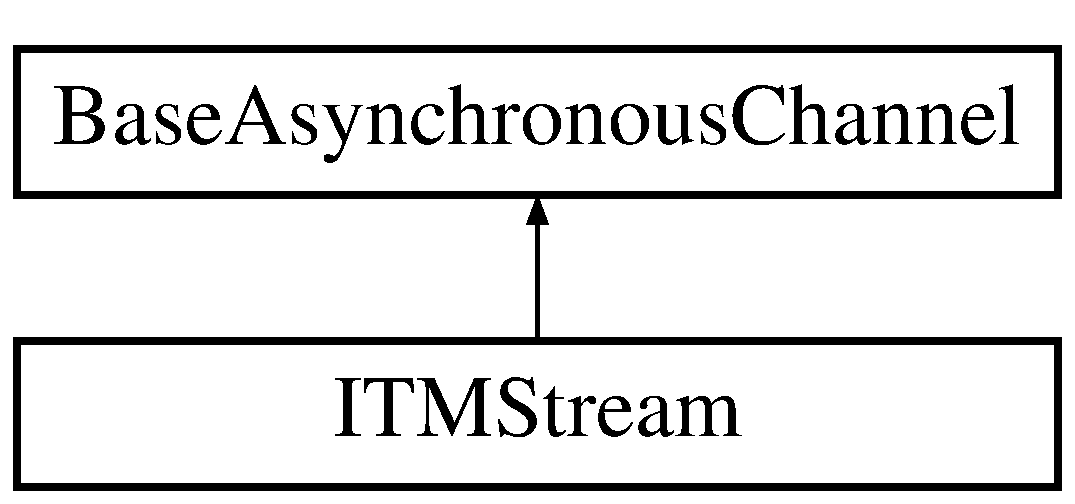
\includegraphics[height=2.000000cm]{structITMStream}
\end{center}
\end{figure}
\subsection*{Public Attributes}
\begin{DoxyCompactItemize}
\item 
\hypertarget{structITMStream_a243b326e52dc6ffcc22e5ecabb2a3e2a}{const struct \hyperlink{structITMStreamVMT}{I\+T\+M\+Stream\+V\+M\+T} $\ast$ \hyperlink{structITMStream_a243b326e52dc6ffcc22e5ecabb2a3e2a}{vmt}}\label{structITMStream_a243b326e52dc6ffcc22e5ecabb2a3e2a}

\begin{DoxyCompactList}\small\item\em Virtual Methods Table. \end{DoxyCompactList}\end{DoxyCompactItemize}


\subsection{Detailed Description}
Full duplex itm driver class. 

This class extends {\ttfamily Base\+Asynchronous\+Channel} by adding physical I/\+O queues. 

The documentation for this struct was generated from the following file\+:\begin{DoxyCompactItemize}
\item 
\hyperlink{ITM__trace_8h}{I\+T\+M\+\_\+trace.\+h}\end{DoxyCompactItemize}

\hypertarget{structITMStreamVMT}{\section{I\+T\+M\+Stream\+V\+M\+T Struct Reference}
\label{structITMStreamVMT}\index{I\+T\+M\+Stream\+V\+M\+T@{I\+T\+M\+Stream\+V\+M\+T}}
}


{\ttfamily itm\+Stream} virtual methods table.  




{\ttfamily \#include $<$I\+T\+M\+\_\+trace.\+h$>$}

Inheritance diagram for I\+T\+M\+Stream\+V\+M\+T\+:\begin{figure}[H]
\begin{center}
\leavevmode
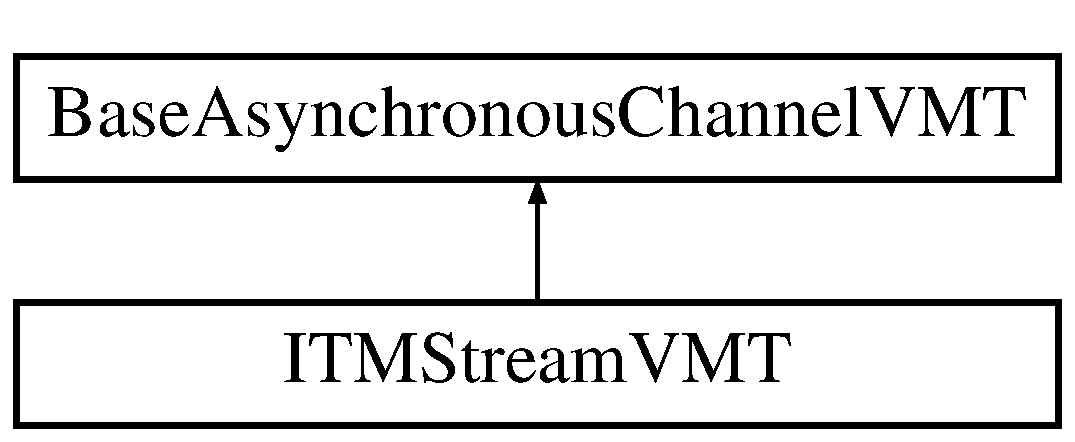
\includegraphics[height=2.000000cm]{structITMStreamVMT}
\end{center}
\end{figure}


\subsection{Detailed Description}
{\ttfamily itm\+Stream} virtual methods table. 

The documentation for this struct was generated from the following file\+:\begin{DoxyCompactItemize}
\item 
\hyperlink{ITM__trace_8h}{I\+T\+M\+\_\+trace.\+h}\end{DoxyCompactItemize}

\hypertarget{structlcfg}{\section{lcfg Struct Reference}
\label{structlcfg}\index{lcfg@{lcfg}}
}
\subsection*{Public Attributes}
\begin{DoxyCompactItemize}
\item 
\hypertarget{structlcfg_a85ae9529e15e58a116ba52bced27f548}{char {\bfseries error} \mbox{[}0xff\mbox{]}}\label{structlcfg_a85ae9529e15e58a116ba52bced27f548}

\item 
\hypertarget{structlcfg_a628a554c42296771f9ff81c69d677ce3}{struct \hyperlink{structlcfg__parser}{lcfg\+\_\+parser} $\ast$ {\bfseries parser}}\label{structlcfg_a628a554c42296771f9ff81c69d677ce3}

\end{DoxyCompactItemize}


The documentation for this struct was generated from the following file\+:\begin{DoxyCompactItemize}
\item 
lcfg\+\_\+static.\+c\end{DoxyCompactItemize}

\hypertarget{structlcfg__parser}{\section{lcfg\+\_\+parser Struct Reference}
\label{structlcfg__parser}\index{lcfg\+\_\+parser@{lcfg\+\_\+parser}}
}
\subsection*{Public Attributes}
\begin{DoxyCompactItemize}
\item 
\hypertarget{structlcfg__parser_a4a9b24160b18516d283c913296e0b90d}{struct \hyperlink{structlcfg}{lcfg} $\ast$ {\bfseries lcfg}}\label{structlcfg__parser_a4a9b24160b18516d283c913296e0b90d}

\item 
\hypertarget{structlcfg__parser_a2667151d72fd3ca8b241676834b891ce}{char $\ast$ {\bfseries filename}}\label{structlcfg__parser_a2667151d72fd3ca8b241676834b891ce}

\item 
\hypertarget{structlcfg__parser_ae86982303a26985e6dae7275b4624661}{struct \hyperlink{structlcfg__scanner}{lcfg\+\_\+scanner} $\ast$ {\bfseries scanner}}\label{structlcfg__parser_ae86982303a26985e6dae7275b4624661}

\item 
\hypertarget{structlcfg__parser_a75354cd041b465f1c3fea34802de325d}{struct \hyperlink{structlcfg__parser__value__pair}{lcfg\+\_\+parser\+\_\+value\+\_\+pair} $\ast$ {\bfseries values}}\label{structlcfg__parser_a75354cd041b465f1c3fea34802de325d}

\item 
\hypertarget{structlcfg__parser_a32a233c04751695ed1e3103f7538a083}{unsigned int {\bfseries value\+\_\+length}}\label{structlcfg__parser_a32a233c04751695ed1e3103f7538a083}

\item 
\hypertarget{structlcfg__parser_a2a0d8e132480cdd173ffd2040302121f}{unsigned int {\bfseries value\+\_\+capacity}}\label{structlcfg__parser_a2a0d8e132480cdd173ffd2040302121f}

\end{DoxyCompactItemize}


The documentation for this struct was generated from the following file\+:\begin{DoxyCompactItemize}
\item 
lcfg\+\_\+static.\+c\end{DoxyCompactItemize}

\hypertarget{structlcfg__parser__value__pair}{\section{lcfg\+\_\+parser\+\_\+value\+\_\+pair Struct Reference}
\label{structlcfg__parser__value__pair}\index{lcfg\+\_\+parser\+\_\+value\+\_\+pair@{lcfg\+\_\+parser\+\_\+value\+\_\+pair}}
}
\subsection*{Public Attributes}
\begin{DoxyCompactItemize}
\item 
\hypertarget{structlcfg__parser__value__pair_af285c1ce4cf893f06ac6fe2567e5d6d2}{char $\ast$ {\bfseries key}}\label{structlcfg__parser__value__pair_af285c1ce4cf893f06ac6fe2567e5d6d2}

\item 
\hypertarget{structlcfg__parser__value__pair_a53dd94b220d778f307b6aa265b469c11}{struct \hyperlink{structlcfg__string}{lcfg\+\_\+string} $\ast$ {\bfseries value}}\label{structlcfg__parser__value__pair_a53dd94b220d778f307b6aa265b469c11}

\end{DoxyCompactItemize}


The documentation for this struct was generated from the following file\+:\begin{DoxyCompactItemize}
\item 
lcfg\+\_\+static.\+c\end{DoxyCompactItemize}

\hypertarget{structlcfg__scanner}{\section{lcfg\+\_\+scanner Struct Reference}
\label{structlcfg__scanner}\index{lcfg\+\_\+scanner@{lcfg\+\_\+scanner}}
}
\subsection*{Public Attributes}
\begin{DoxyCompactItemize}
\item 
\hypertarget{structlcfg__scanner_af937d1611322ec0f7639e584df7b96c0}{struct \hyperlink{structlcfg}{lcfg} $\ast$ {\bfseries lcfg}}\label{structlcfg__scanner_af937d1611322ec0f7639e584df7b96c0}

\item 
\hypertarget{structlcfg__scanner_ac7f8214cb39c68f07276afa07a68d08a}{int {\bfseries fd}}\label{structlcfg__scanner_ac7f8214cb39c68f07276afa07a68d08a}

\item 
\hypertarget{structlcfg__scanner_a394a3bf2df622e0e698884f06e8d68c8}{char {\bfseries buffer} \mbox{[}B\+U\+F\+F\+E\+R\+\_\+\+S\+I\+Z\+E\mbox{]}}\label{structlcfg__scanner_a394a3bf2df622e0e698884f06e8d68c8}

\item 
\hypertarget{structlcfg__scanner_a25753fe2275eba8bee3f994c5af1a192}{int {\bfseries offset}}\label{structlcfg__scanner_a25753fe2275eba8bee3f994c5af1a192}

\item 
\hypertarget{structlcfg__scanner_aa3da8cfe3f1a26f13bd2d3ae5e080393}{int {\bfseries size}}\label{structlcfg__scanner_aa3da8cfe3f1a26f13bd2d3ae5e080393}

\item 
\hypertarget{structlcfg__scanner_aa7b1358559f5608fcbca98936cdd9cdb}{int {\bfseries eof}}\label{structlcfg__scanner_aa7b1358559f5608fcbca98936cdd9cdb}

\item 
\hypertarget{structlcfg__scanner_a42442806f225004bfb3e00c05ab5e37a}{short {\bfseries line}}\label{structlcfg__scanner_a42442806f225004bfb3e00c05ab5e37a}

\item 
\hypertarget{structlcfg__scanner_ae0d696370027e1104574e62b7603c2b4}{short {\bfseries col}}\label{structlcfg__scanner_ae0d696370027e1104574e62b7603c2b4}

\item 
\hypertarget{structlcfg__scanner_ab0350457b83dd5b4d9720cfde3266144}{struct \hyperlink{structlcfg__token}{lcfg\+\_\+token} {\bfseries prepared\+\_\+token}}\label{structlcfg__scanner_ab0350457b83dd5b4d9720cfde3266144}

\item 
\hypertarget{structlcfg__scanner_a3975f5b241ca65656110c96f7f009d02}{int {\bfseries token\+\_\+eof}}\label{structlcfg__scanner_a3975f5b241ca65656110c96f7f009d02}

\end{DoxyCompactItemize}


The documentation for this struct was generated from the following file\+:\begin{DoxyCompactItemize}
\item 
lcfg\+\_\+static.\+c\end{DoxyCompactItemize}

\hypertarget{structlcfg__string}{\section{lcfg\+\_\+string Struct Reference}
\label{structlcfg__string}\index{lcfg\+\_\+string@{lcfg\+\_\+string}}
}
\subsection*{Public Attributes}
\begin{DoxyCompactItemize}
\item 
\hypertarget{structlcfg__string_af9f8a270270c71a3ec2448369639f6f4}{char $\ast$ {\bfseries str}}\label{structlcfg__string_af9f8a270270c71a3ec2448369639f6f4}

\item 
\hypertarget{structlcfg__string_ad6fff99c12b91f5ccb7468cb50463c49}{unsigned int {\bfseries size}}\label{structlcfg__string_ad6fff99c12b91f5ccb7468cb50463c49}

\item 
\hypertarget{structlcfg__string_aa37e32181d18ca021994923fa80933b6}{unsigned int {\bfseries capacity}}\label{structlcfg__string_aa37e32181d18ca021994923fa80933b6}

\end{DoxyCompactItemize}


The documentation for this struct was generated from the following file\+:\begin{DoxyCompactItemize}
\item 
lcfg\+\_\+static.\+c\end{DoxyCompactItemize}

\hypertarget{structlcfg__token}{\section{lcfg\+\_\+token Struct Reference}
\label{structlcfg__token}\index{lcfg\+\_\+token@{lcfg\+\_\+token}}
}
\subsection*{Public Attributes}
\begin{DoxyCompactItemize}
\item 
\hypertarget{structlcfg__token_ae8b2ce5dae400305af6c25688f4d186a}{enum lcfg\+\_\+token\+\_\+type {\bfseries type}}\label{structlcfg__token_ae8b2ce5dae400305af6c25688f4d186a}

\item 
\hypertarget{structlcfg__token_a270e92599188eeb2de7255193528e7fa}{struct \hyperlink{structlcfg__string}{lcfg\+\_\+string} $\ast$ {\bfseries string}}\label{structlcfg__token_a270e92599188eeb2de7255193528e7fa}

\item 
\hypertarget{structlcfg__token_a767e59f04dcbfe96de0a369b951e024c}{short {\bfseries line}}\label{structlcfg__token_a767e59f04dcbfe96de0a369b951e024c}

\item 
\hypertarget{structlcfg__token_a95b60fff70bf893c69041802e76f4d6b}{short {\bfseries col}}\label{structlcfg__token_a95b60fff70bf893c69041802e76f4d6b}

\end{DoxyCompactItemize}


The documentation for this struct was generated from the following file\+:\begin{DoxyCompactItemize}
\item 
lcfg\+\_\+static.\+c\end{DoxyCompactItemize}

\hypertarget{structlcfgx__tree__node}{\section{lcfgx\+\_\+tree\+\_\+node Struct Reference}
\label{structlcfgx__tree__node}\index{lcfgx\+\_\+tree\+\_\+node@{lcfgx\+\_\+tree\+\_\+node}}
}
\subsection*{Public Attributes}
\begin{DoxyCompactItemize}
\item 
\hypertarget{structlcfgx__tree__node_a803c7d39158d9a162d2ba98706d73e2f}{enum lcfgx\+\_\+type {\bfseries type}}\label{structlcfgx__tree__node_a803c7d39158d9a162d2ba98706d73e2f}

\item 
\hypertarget{structlcfgx__tree__node_a9ad38b21d802ff3303c814ab35490355}{char $\ast$ {\bfseries key}}\label{structlcfgx__tree__node_a9ad38b21d802ff3303c814ab35490355}

\item 
\hypertarget{structlcfgx__tree__node_ac8fcfa869f0c4a4ee426c93a3b39246d}{\begin{tabbing}
xx\=xx\=xx\=xx\=xx\=xx\=xx\=xx\=xx\=\kill
union \{\\
\>struct \{\\
\>\>void $\ast$ {\bfseries data}\\
\>\>size\_t {\bfseries len}\\
\>\} {\bfseries string}\\
\>struct \hyperlink{structlcfgx__tree__node}{lcfgx\_tree\_node} $\ast$ {\bfseries elements}\\
\} {\bfseries value}}\label{structlcfgx__tree__node_ac8fcfa869f0c4a4ee426c93a3b39246d}
\\

\end{tabbing}\item 
\hypertarget{structlcfgx__tree__node_aa1820adf2213750b5de1d2ce87206563}{struct \hyperlink{structlcfgx__tree__node}{lcfgx\+\_\+tree\+\_\+node} $\ast$ {\bfseries next}}\label{structlcfgx__tree__node_aa1820adf2213750b5de1d2ce87206563}

\end{DoxyCompactItemize}


The documentation for this struct was generated from the following file\+:\begin{DoxyCompactItemize}
\item 
lcfg\+\_\+static.\+h\end{DoxyCompactItemize}

\chapter{File Documentation}
\hypertarget{ArrayList_8h}{\section{Array\+List.\+h File Reference}
\label{ArrayList_8h}\index{Array\+List.\+h@{Array\+List.\+h}}
}


List all modbus slaves in an array.  


{\ttfamily \#include $<$stdint.\+h$>$}\\*
\subsection*{Classes}
\begin{DoxyCompactItemize}
\item 
struct \hyperlink{structDeviceElement}{Device\+Element}
\item 
struct \hyperlink{structDeviceList}{Device\+List}
\end{DoxyCompactItemize}
\subsection*{Enumerations}
\begin{DoxyCompactItemize}
\item 
\hypertarget{ArrayList_8h_a10275a078bd1abcbebc206cc5d19e18b}{enum {\bfseries connection} \{ {\bfseries C\+O\+N\+N\+E\+C\+T\+E\+D}, 
{\bfseries C\+O\+N\+N\+E\+C\+T\+I\+O\+N\+L\+E\+S\+S}
 \}}\label{ArrayList_8h_a10275a078bd1abcbebc206cc5d19e18b}

\item 
\hypertarget{ArrayList_8h_aabddd589ce7fd3d829e15265d92dbedc}{enum {\bfseries Shift} \{ {\bfseries R\+I\+G\+H\+T}, 
{\bfseries L\+E\+F\+T}
 \}}\label{ArrayList_8h_aabddd589ce7fd3d829e15265d92dbedc}

\end{DoxyCompactItemize}
\subsection*{Functions}
\begin{DoxyCompactItemize}
\item 
void \hyperlink{ArrayList_8h_a8fdce5bbae69fb47b47d1d180bb684e8}{init} (\hyperlink{structDeviceList}{Device\+List} $\ast$const)
\begin{DoxyCompactList}\small\item\em init \end{DoxyCompactList}\item 
void \hyperlink{ArrayList_8h_afb06e16b078fcf677e9e4885b930b6ca}{init\+With\+Size} (\hyperlink{structDeviceList}{Device\+List} $\ast$const, int)
\begin{DoxyCompactList}\small\item\em init\+With\+Size \end{DoxyCompactList}\item 
void \hyperlink{ArrayList_8h_a185e68630c9173196c1edd660be0f39f}{init\+With\+Size\+And\+Inc\+Rate} (\hyperlink{structDeviceList}{Device\+List} $\ast$const, int, int)
\begin{DoxyCompactList}\small\item\em init\+With\+Size\+And\+Inc\+Rate \end{DoxyCompactList}\item 
void \hyperlink{ArrayList_8h_a0da485f357f2e300cd9f548ab8c76a13}{clean} (\hyperlink{structDeviceList}{Device\+List} $\ast$)
\begin{DoxyCompactList}\small\item\em clean \end{DoxyCompactList}\item 
int \hyperlink{ArrayList_8h_a79e90e1dcb968556973ee8be8796471d}{add} (\hyperlink{structDeviceList}{Device\+List} $\ast$const, \hyperlink{structDeviceElement}{Device\+Element})
\begin{DoxyCompactList}\small\item\em add \end{DoxyCompactList}\item 
int \hyperlink{ArrayList_8h_a696a8624ae12235c5d8b33f3377961a8}{insert} (\hyperlink{structDeviceList}{Device\+List} $\ast$const, \hyperlink{structDeviceElement}{Device\+Element}, int)
\begin{DoxyCompactList}\small\item\em insert \end{DoxyCompactList}\item 
int \hyperlink{ArrayList_8h_ac70cf2aea8c4ec9df0b1873d0930e260}{populate} (\hyperlink{structDeviceList}{Device\+List} $\ast$const, \hyperlink{structDeviceElement}{Device\+Element} e)
\begin{DoxyCompactList}\small\item\em populate \end{DoxyCompactList}\item 
\hyperlink{structDeviceElement}{Device\+Element} $\ast$ \hyperlink{ArrayList_8h_a1787a27dad405da153e7497128e79131}{remove\+At} (\hyperlink{structDeviceList}{Device\+List} $\ast$const, int)
\begin{DoxyCompactList}\small\item\em remove\+At \end{DoxyCompactList}\item 
void \hyperlink{ArrayList_8h_a98f2b422f7738949d22a5982e3158dc8}{clear} (\hyperlink{structDeviceList}{Device\+List} $\ast$const)
\begin{DoxyCompactList}\small\item\em clear \end{DoxyCompactList}\item 
int \hyperlink{ArrayList_8h_a70c9ad8bc50a1b95c0562f5dcf2beb25}{set} (\hyperlink{structDeviceList}{Device\+List} $\ast$const, \hyperlink{structDeviceElement}{Device\+Element}, int)
\begin{DoxyCompactList}\small\item\em set \end{DoxyCompactList}\item 
\hyperlink{structDeviceElement}{Device\+Element} $\ast$ \hyperlink{ArrayList_8h_a380b18844b8a55adcfffdcc53a0e44a7}{get} (\hyperlink{structDeviceList}{Device\+List} $\ast$const, int)
\begin{DoxyCompactList}\small\item\em get \end{DoxyCompactList}\item 
int \hyperlink{ArrayList_8h_af0238a455e5a3a6e6bffb9552c21d93f}{get\+\_\+\+Index} (\hyperlink{structDeviceList}{Device\+List} $\ast$const, int8\+\_\+t)
\begin{DoxyCompactList}\small\item\em get\+\_\+\+Index \end{DoxyCompactList}\item 
void \hyperlink{ArrayList_8h_a68775a9a1eb8997399fce958cef29d58}{print} (const \hyperlink{structDeviceList}{Device\+List} $\ast$const)
\begin{DoxyCompactList}\small\item\em print \end{DoxyCompactList}\item 
int \hyperlink{ArrayList_8h_aed33b24830648cf4495456b524602aff}{last\+Index\+Of} (const \hyperlink{structDeviceList}{Device\+List} $\ast$const, \hyperlink{structDeviceElement}{Device\+Element})
\begin{DoxyCompactList}\small\item\em last\+Index\+Of \end{DoxyCompactList}\item 
int \hyperlink{ArrayList_8h_a86a2ab4ab89478f17bf26b1b25012c3c}{index\+Of} (const \hyperlink{structDeviceList}{Device\+List} $\ast$const, \hyperlink{structDeviceElement}{Device\+Element})
\begin{DoxyCompactList}\small\item\em index\+Of \end{DoxyCompactList}\item 
int \hyperlink{ArrayList_8h_a786244154ce41407a3b11562de3e1305}{is\+Empty} (const \hyperlink{structDeviceList}{Device\+List} $\ast$const)
\begin{DoxyCompactList}\small\item\em is\+Empty \end{DoxyCompactList}\end{DoxyCompactItemize}


\subsection{Detailed Description}
List all modbus slaves in an array. 

Details. 

\subsection{Function Documentation}
\hypertarget{ArrayList_8h_a79e90e1dcb968556973ee8be8796471d}{\index{Array\+List.\+h@{Array\+List.\+h}!add@{add}}
\index{add@{add}!Array\+List.\+h@{Array\+List.\+h}}
\subsubsection[{add}]{\setlength{\rightskip}{0pt plus 5cm}int add (
\begin{DoxyParamCaption}
\item[{{\bf Device\+List} $\ast$}]{const, }
\item[{{\bf Device\+Element}}]{}
\end{DoxyParamCaption}
)}}\label{ArrayList_8h_a79e90e1dcb968556973ee8be8796471d}


add 


\begin{DoxyParams}{Parameters}
{\em list} & Array\+List \\
\hline
{\em \hyperlink{structDeviceElement}{Device\+Element}} & data\\
\hline
\end{DoxyParams}
\begin{DoxyReturn}{Returns}
integer 
\end{DoxyReturn}
\hypertarget{ArrayList_8h_a0da485f357f2e300cd9f548ab8c76a13}{\index{Array\+List.\+h@{Array\+List.\+h}!clean@{clean}}
\index{clean@{clean}!Array\+List.\+h@{Array\+List.\+h}}
\subsubsection[{clean}]{\setlength{\rightskip}{0pt plus 5cm}void clean (
\begin{DoxyParamCaption}
\item[{{\bf Device\+List} $\ast$}]{}
\end{DoxyParamCaption}
)}}\label{ArrayList_8h_a0da485f357f2e300cd9f548ab8c76a13}


clean 


\begin{DoxyParams}{Parameters}
{\em list} & Array\+List\\
\hline
\end{DoxyParams}
\begin{DoxyReturn}{Returns}
none 
\end{DoxyReturn}
\hypertarget{ArrayList_8h_a98f2b422f7738949d22a5982e3158dc8}{\index{Array\+List.\+h@{Array\+List.\+h}!clear@{clear}}
\index{clear@{clear}!Array\+List.\+h@{Array\+List.\+h}}
\subsubsection[{clear}]{\setlength{\rightskip}{0pt plus 5cm}void clear (
\begin{DoxyParamCaption}
\item[{{\bf Device\+List} $\ast$}]{const}
\end{DoxyParamCaption}
)}}\label{ArrayList_8h_a98f2b422f7738949d22a5982e3158dc8}


clear 


\begin{DoxyParams}{Parameters}
{\em list} & Array\+List\\
\hline
\end{DoxyParams}
\begin{DoxyReturn}{Returns}
none 
\end{DoxyReturn}
\hypertarget{ArrayList_8h_a380b18844b8a55adcfffdcc53a0e44a7}{\index{Array\+List.\+h@{Array\+List.\+h}!get@{get}}
\index{get@{get}!Array\+List.\+h@{Array\+List.\+h}}
\subsubsection[{get}]{\setlength{\rightskip}{0pt plus 5cm}{\bf Device\+Element}$\ast$ get (
\begin{DoxyParamCaption}
\item[{{\bf Device\+List} $\ast$}]{const, }
\item[{int}]{}
\end{DoxyParamCaption}
)}}\label{ArrayList_8h_a380b18844b8a55adcfffdcc53a0e44a7}


get 


\begin{DoxyParams}{Parameters}
{\em list} & Array\+List \\
\hline
{\em index} & index in list\\
\hline
\end{DoxyParams}
\begin{DoxyReturn}{Returns}
\hyperlink{structDeviceElement}{Device\+Element} 
\end{DoxyReturn}
\hypertarget{ArrayList_8h_af0238a455e5a3a6e6bffb9552c21d93f}{\index{Array\+List.\+h@{Array\+List.\+h}!get\+\_\+\+Index@{get\+\_\+\+Index}}
\index{get\+\_\+\+Index@{get\+\_\+\+Index}!Array\+List.\+h@{Array\+List.\+h}}
\subsubsection[{get\+\_\+\+Index}]{\setlength{\rightskip}{0pt plus 5cm}int get\+\_\+\+Index (
\begin{DoxyParamCaption}
\item[{{\bf Device\+List} $\ast$}]{const, }
\item[{int8\+\_\+t}]{}
\end{DoxyParamCaption}
)}}\label{ArrayList_8h_af0238a455e5a3a6e6bffb9552c21d93f}


get\+\_\+\+Index 


\begin{DoxyParams}{Parameters}
{\em list} & Array\+List \\
\hline
{\em address} & Element.\+address\\
\hline
\end{DoxyParams}
\begin{DoxyReturn}{Returns}
Index 
\end{DoxyReturn}
\hypertarget{ArrayList_8h_a86a2ab4ab89478f17bf26b1b25012c3c}{\index{Array\+List.\+h@{Array\+List.\+h}!index\+Of@{index\+Of}}
\index{index\+Of@{index\+Of}!Array\+List.\+h@{Array\+List.\+h}}
\subsubsection[{index\+Of}]{\setlength{\rightskip}{0pt plus 5cm}int index\+Of (
\begin{DoxyParamCaption}
\item[{const {\bf Device\+List} $\ast$}]{const, }
\item[{{\bf Device\+Element}}]{}
\end{DoxyParamCaption}
)}}\label{ArrayList_8h_a86a2ab4ab89478f17bf26b1b25012c3c}


index\+Of 


\begin{DoxyParams}{Parameters}
{\em list} & Array\+List \\
\hline
{\em \hyperlink{structDeviceElement}{Device\+Element}} & data\\
\hline
\end{DoxyParams}
\begin{DoxyReturn}{Returns}
integer 
\end{DoxyReturn}
\hypertarget{ArrayList_8h_a8fdce5bbae69fb47b47d1d180bb684e8}{\index{Array\+List.\+h@{Array\+List.\+h}!init@{init}}
\index{init@{init}!Array\+List.\+h@{Array\+List.\+h}}
\subsubsection[{init}]{\setlength{\rightskip}{0pt plus 5cm}void init (
\begin{DoxyParamCaption}
\item[{{\bf Device\+List} $\ast$}]{const}
\end{DoxyParamCaption}
)}}\label{ArrayList_8h_a8fdce5bbae69fb47b47d1d180bb684e8}


init 


\begin{DoxyParams}{Parameters}
{\em list} & Array\+List\\
\hline
\end{DoxyParams}
\begin{DoxyReturn}{Returns}
none 
\end{DoxyReturn}
\hypertarget{ArrayList_8h_afb06e16b078fcf677e9e4885b930b6ca}{\index{Array\+List.\+h@{Array\+List.\+h}!init\+With\+Size@{init\+With\+Size}}
\index{init\+With\+Size@{init\+With\+Size}!Array\+List.\+h@{Array\+List.\+h}}
\subsubsection[{init\+With\+Size}]{\setlength{\rightskip}{0pt plus 5cm}void init\+With\+Size (
\begin{DoxyParamCaption}
\item[{{\bf Device\+List} $\ast$}]{const, }
\item[{int}]{}
\end{DoxyParamCaption}
)}}\label{ArrayList_8h_afb06e16b078fcf677e9e4885b930b6ca}


init\+With\+Size 


\begin{DoxyParams}{Parameters}
{\em list} & Array\+List \\
\hline
{\em size} & size of list\\
\hline
\end{DoxyParams}
\begin{DoxyReturn}{Returns}
none 
\end{DoxyReturn}
\hypertarget{ArrayList_8h_a185e68630c9173196c1edd660be0f39f}{\index{Array\+List.\+h@{Array\+List.\+h}!init\+With\+Size\+And\+Inc\+Rate@{init\+With\+Size\+And\+Inc\+Rate}}
\index{init\+With\+Size\+And\+Inc\+Rate@{init\+With\+Size\+And\+Inc\+Rate}!Array\+List.\+h@{Array\+List.\+h}}
\subsubsection[{init\+With\+Size\+And\+Inc\+Rate}]{\setlength{\rightskip}{0pt plus 5cm}void init\+With\+Size\+And\+Inc\+Rate (
\begin{DoxyParamCaption}
\item[{{\bf Device\+List} $\ast$}]{const, }
\item[{int}]{, }
\item[{int}]{}
\end{DoxyParamCaption}
)}}\label{ArrayList_8h_a185e68630c9173196c1edd660be0f39f}


init\+With\+Size\+And\+Inc\+Rate 


\begin{DoxyParams}{Parameters}
{\em list} & Array\+List \\
\hline
{\em size} & size of list \\
\hline
{\em rate} & increment rate\\
\hline
\end{DoxyParams}
\begin{DoxyReturn}{Returns}
none 
\end{DoxyReturn}
\hypertarget{ArrayList_8h_a696a8624ae12235c5d8b33f3377961a8}{\index{Array\+List.\+h@{Array\+List.\+h}!insert@{insert}}
\index{insert@{insert}!Array\+List.\+h@{Array\+List.\+h}}
\subsubsection[{insert}]{\setlength{\rightskip}{0pt plus 5cm}int insert (
\begin{DoxyParamCaption}
\item[{{\bf Device\+List} $\ast$}]{const, }
\item[{{\bf Device\+Element}}]{, }
\item[{int}]{}
\end{DoxyParamCaption}
)}}\label{ArrayList_8h_a696a8624ae12235c5d8b33f3377961a8}


insert 


\begin{DoxyParams}{Parameters}
{\em list} & Array\+List \\
\hline
{\em \hyperlink{structDeviceElement}{Device\+Element}} & data \\
\hline
{\em index} & index in list\\
\hline
\end{DoxyParams}
\begin{DoxyReturn}{Returns}
integer 
\end{DoxyReturn}
\hypertarget{ArrayList_8h_a786244154ce41407a3b11562de3e1305}{\index{Array\+List.\+h@{Array\+List.\+h}!is\+Empty@{is\+Empty}}
\index{is\+Empty@{is\+Empty}!Array\+List.\+h@{Array\+List.\+h}}
\subsubsection[{is\+Empty}]{\setlength{\rightskip}{0pt plus 5cm}int is\+Empty (
\begin{DoxyParamCaption}
\item[{const {\bf Device\+List} $\ast$}]{const}
\end{DoxyParamCaption}
)}}\label{ArrayList_8h_a786244154ce41407a3b11562de3e1305}


is\+Empty 


\begin{DoxyParams}{Parameters}
{\em list} & Array\+List\\
\hline
\end{DoxyParams}
\begin{DoxyReturn}{Returns}
integer 
\end{DoxyReturn}
\hypertarget{ArrayList_8h_aed33b24830648cf4495456b524602aff}{\index{Array\+List.\+h@{Array\+List.\+h}!last\+Index\+Of@{last\+Index\+Of}}
\index{last\+Index\+Of@{last\+Index\+Of}!Array\+List.\+h@{Array\+List.\+h}}
\subsubsection[{last\+Index\+Of}]{\setlength{\rightskip}{0pt plus 5cm}int last\+Index\+Of (
\begin{DoxyParamCaption}
\item[{const {\bf Device\+List} $\ast$}]{const, }
\item[{{\bf Device\+Element}}]{}
\end{DoxyParamCaption}
)}}\label{ArrayList_8h_aed33b24830648cf4495456b524602aff}


last\+Index\+Of 


\begin{DoxyParams}{Parameters}
{\em list} & Array\+List \\
\hline
{\em \hyperlink{structDeviceElement}{Device\+Element}} & data\\
\hline
\end{DoxyParams}
\begin{DoxyReturn}{Returns}
integer 
\end{DoxyReturn}
\hypertarget{ArrayList_8h_ac70cf2aea8c4ec9df0b1873d0930e260}{\index{Array\+List.\+h@{Array\+List.\+h}!populate@{populate}}
\index{populate@{populate}!Array\+List.\+h@{Array\+List.\+h}}
\subsubsection[{populate}]{\setlength{\rightskip}{0pt plus 5cm}int populate (
\begin{DoxyParamCaption}
\item[{{\bf Device\+List} $\ast$}]{const, }
\item[{{\bf Device\+Element}}]{e}
\end{DoxyParamCaption}
)}}\label{ArrayList_8h_ac70cf2aea8c4ec9df0b1873d0930e260}


populate 


\begin{DoxyParams}{Parameters}
{\em list} & Array\+List \\
\hline
{\em address} & slave address\\
\hline
\end{DoxyParams}
\begin{DoxyReturn}{Returns}
integer 
\end{DoxyReturn}
\hypertarget{ArrayList_8h_a68775a9a1eb8997399fce958cef29d58}{\index{Array\+List.\+h@{Array\+List.\+h}!print@{print}}
\index{print@{print}!Array\+List.\+h@{Array\+List.\+h}}
\subsubsection[{print}]{\setlength{\rightskip}{0pt plus 5cm}void print (
\begin{DoxyParamCaption}
\item[{const {\bf Device\+List} $\ast$}]{const}
\end{DoxyParamCaption}
)}}\label{ArrayList_8h_a68775a9a1eb8997399fce958cef29d58}


print 


\begin{DoxyParams}{Parameters}
{\em list} & Array\+List\\
\hline
\end{DoxyParams}
\begin{DoxyReturn}{Returns}
none 
\end{DoxyReturn}
\hypertarget{ArrayList_8h_a1787a27dad405da153e7497128e79131}{\index{Array\+List.\+h@{Array\+List.\+h}!remove\+At@{remove\+At}}
\index{remove\+At@{remove\+At}!Array\+List.\+h@{Array\+List.\+h}}
\subsubsection[{remove\+At}]{\setlength{\rightskip}{0pt plus 5cm}{\bf Device\+Element}$\ast$ remove\+At (
\begin{DoxyParamCaption}
\item[{{\bf Device\+List} $\ast$}]{const, }
\item[{int}]{}
\end{DoxyParamCaption}
)}}\label{ArrayList_8h_a1787a27dad405da153e7497128e79131}


remove\+At 


\begin{DoxyParams}{Parameters}
{\em list} & Array\+List \\
\hline
{\em index} & index in list\\
\hline
\end{DoxyParams}
\begin{DoxyReturn}{Returns}
\hyperlink{structDeviceElement}{Device\+Element} 
\end{DoxyReturn}
\hypertarget{ArrayList_8h_a70c9ad8bc50a1b95c0562f5dcf2beb25}{\index{Array\+List.\+h@{Array\+List.\+h}!set@{set}}
\index{set@{set}!Array\+List.\+h@{Array\+List.\+h}}
\subsubsection[{set}]{\setlength{\rightskip}{0pt plus 5cm}int set (
\begin{DoxyParamCaption}
\item[{{\bf Device\+List} $\ast$}]{const, }
\item[{{\bf Device\+Element}}]{, }
\item[{int}]{}
\end{DoxyParamCaption}
)}}\label{ArrayList_8h_a70c9ad8bc50a1b95c0562f5dcf2beb25}


set 


\begin{DoxyParams}{Parameters}
{\em list} & Array\+List \\
\hline
{\em \hyperlink{structDeviceElement}{Device\+Element}} & data \\
\hline
{\em index} & index in list\\
\hline
\end{DoxyParams}
\begin{DoxyReturn}{Returns}
integer 
\end{DoxyReturn}

\hypertarget{ITM__trace_8c}{\section{I\+T\+M\+\_\+trace.\+c File Reference}
\label{ITM__trace_8c}\index{I\+T\+M\+\_\+trace.\+c@{I\+T\+M\+\_\+trace.\+c}}
}


I\+T\+M Driver code.  


{\ttfamily \#include \char`\"{}hal.\+h\char`\"{}}\\*
{\ttfamily \#include \char`\"{}I\+T\+M\+\_\+trace.\+h\char`\"{}}\\*
\subsection*{Functions}
\begin{DoxyCompactItemize}
\item 
\hypertarget{group__ITM_gafc909eadbc17807bfc2c95d22988e396}{void {\bfseries Debug\+\_\+\+I\+T\+M\+Debug\+Output\+Char} (char ch)}\label{group__ITM_gafc909eadbc17807bfc2c95d22988e396}

\item 
void \hyperlink{group__ITM_gab43f2808bf17b6e393e95faee2abd058}{itm\+Object\+Init} (\hyperlink{structITMStream}{I\+T\+M\+Stream} $\ast$pitm)
\begin{DoxyCompactList}\small\item\em I\+T\+M stream object initialization. \end{DoxyCompactList}\end{DoxyCompactItemize}


\subsection{Detailed Description}
I\+T\+M Driver code. 


\hypertarget{ITM__trace_8h}{\section{I\+T\+M\+\_\+trace.\+h File Reference}
\label{ITM__trace_8h}\index{I\+T\+M\+\_\+trace.\+h@{I\+T\+M\+\_\+trace.\+h}}
}


I\+T\+M Driver macros and structures.  


\subsection*{Classes}
\begin{DoxyCompactItemize}
\item 
struct \hyperlink{structITMStreamVMT}{I\+T\+M\+Stream\+V\+M\+T}
\begin{DoxyCompactList}\small\item\em {\ttfamily itm\+Stream} virtual methods table. \end{DoxyCompactList}\item 
struct \hyperlink{structITMStream}{I\+T\+M\+Stream}
\begin{DoxyCompactList}\small\item\em Full duplex itm driver class. \end{DoxyCompactList}\end{DoxyCompactItemize}
\subsection*{Macros}
\begin{DoxyCompactItemize}
\item 
\hypertarget{group__ITM_ga2499678d2188c663196fecc40bd35483}{\#define \hyperlink{group__ITM_ga2499678d2188c663196fecc40bd35483}{\+\_\+itm\+\_\+stream\+\_\+data}~\+\_\+base\+\_\+sequential\+\_\+stream\+\_\+data}\label{group__ITM_ga2499678d2188c663196fecc40bd35483}

\begin{DoxyCompactList}\small\item\em {\ttfamily itm\+Stream} specific data. \end{DoxyCompactList}\end{DoxyCompactItemize}
\subsection*{Functions}
\begin{DoxyCompactItemize}
\item 
void \hyperlink{group__ITM_gab43f2808bf17b6e393e95faee2abd058}{itm\+Object\+Init} (\hyperlink{structITMStream}{I\+T\+M\+Stream} $\ast$pitm)
\begin{DoxyCompactList}\small\item\em I\+T\+M stream object initialization. \end{DoxyCompactList}\end{DoxyCompactItemize}


\subsection{Detailed Description}
I\+T\+M Driver macros and structures. 


\hypertarget{lwipopts_8h}{\section{lwipopts.\+h File Reference}
\label{lwipopts_8h}\index{lwipopts.\+h@{lwipopts.\+h}}
}
\subsection*{Macros}
\begin{DoxyCompactItemize}
\item 
\#define \hyperlink{lwipopts_8h_ae85efb3a5fcf8585c94b3c2669978959}{S\+Y\+S\+\_\+\+L\+I\+G\+H\+T\+W\+E\+I\+G\+H\+T\+\_\+\+P\+R\+O\+T}~0
\item 
\#define \hyperlink{lwipopts_8h_ae00ba99de94a5bf84d832be8976df59b}{N\+O\+\_\+\+S\+Y\+S}~0
\item 
\#define \hyperlink{lwipopts_8h_a576dfdb593d10f3be17eaf499a439201}{N\+O\+\_\+\+S\+Y\+S\+\_\+\+N\+O\+\_\+\+T\+I\+M\+E\+R\+S}~0
\item 
\#define \hyperlink{lwipopts_8h_aa1dd57a66b6de8c0593e9e3e8d1411f6}{M\+E\+M\+C\+P\+Y}(dst, src, len)~memcpy(dst,src,len)
\item 
\#define \hyperlink{lwipopts_8h_a8c6e3c1e4f74acb16376188dbf8909ec}{S\+M\+E\+M\+C\+P\+Y}(dst, src, len)~memcpy(dst,src,len)
\item 
\#define \hyperlink{lwipopts_8h_a4ef345cc270912bd2230b1c5ec51dfc8}{M\+E\+M\+\_\+\+L\+I\+B\+C\+\_\+\+M\+A\+L\+L\+O\+C}~0
\item 
\#define \hyperlink{lwipopts_8h_ae93af697d27bbcefa6a28052d90f2f38}{M\+E\+M\+P\+\_\+\+M\+E\+M\+\_\+\+M\+A\+L\+L\+O\+C}~0
\item 
\#define \hyperlink{lwipopts_8h_a97343214666ee6dcb18c0bd77b441ea7}{M\+E\+M\+\_\+\+A\+L\+I\+G\+N\+M\+E\+N\+T}~4
\item 
\#define \hyperlink{lwipopts_8h_a2dcf8c45f945dd0c4301a94700f2112c}{M\+E\+M\+\_\+\+S\+I\+Z\+E}~5600
\item 
\#define \hyperlink{lwipopts_8h_a2e6aaf9504e7018db42014af3942187e}{M\+E\+M\+P\+\_\+\+S\+E\+P\+A\+R\+A\+T\+E\+\_\+\+P\+O\+O\+L\+S}~0
\item 
\#define \hyperlink{lwipopts_8h_a27fdd01194a42fc41a7716b72cdb49e3}{M\+E\+M\+P\+\_\+\+O\+V\+E\+R\+F\+L\+O\+W\+\_\+\+C\+H\+E\+C\+K}~0
\item 
\#define \hyperlink{lwipopts_8h_a0838947193e222a9f46b582e01e5beff}{M\+E\+M\+P\+\_\+\+S\+A\+N\+I\+T\+Y\+\_\+\+C\+H\+E\+C\+K}~0
\item 
\#define \hyperlink{lwipopts_8h_addca3141bc7037241769eb152b6f89ba}{M\+E\+M\+\_\+\+U\+S\+E\+\_\+\+P\+O\+O\+L\+S}~0
\item 
\#define \hyperlink{lwipopts_8h_aba8be68e8fd0716b723ce4569ed89f82}{M\+E\+M\+\_\+\+U\+S\+E\+\_\+\+P\+O\+O\+L\+S\+\_\+\+T\+R\+Y\+\_\+\+B\+I\+G\+G\+E\+R\+\_\+\+P\+O\+O\+L}~0
\item 
\#define \hyperlink{lwipopts_8h_a69de593b8ffd4f1c249f03e48e11983b}{M\+E\+M\+P\+\_\+\+U\+S\+E\+\_\+\+C\+U\+S\+T\+O\+M\+\_\+\+P\+O\+O\+L\+S}~0
\item 
\#define \hyperlink{lwipopts_8h_a0a3ef6098813c103e5aba07da76e15e2}{L\+W\+I\+P\+\_\+\+A\+L\+L\+O\+W\+\_\+\+M\+E\+M\+\_\+\+F\+R\+E\+E\+\_\+\+F\+R\+O\+M\+\_\+\+O\+T\+H\+E\+R\+\_\+\+C\+O\+N\+T\+E\+X\+T}~0
\item 
\#define \hyperlink{lwipopts_8h_a92b30aed958ec59334d936d4ca725418}{M\+E\+M\+P\+\_\+\+N\+U\+M\+\_\+\+P\+B\+U\+F}~32
\item 
\#define \hyperlink{lwipopts_8h_a379bf92ed322cda54cb701337421e0d3}{M\+E\+M\+P\+\_\+\+N\+U\+M\+\_\+\+R\+A\+W\+\_\+\+P\+C\+B}~4
\item 
\#define \hyperlink{lwipopts_8h_a2c416da481ab09bd1ba257b75a0707eb}{M\+E\+M\+P\+\_\+\+N\+U\+M\+\_\+\+U\+D\+P\+\_\+\+P\+C\+B}~4
\item 
\#define \hyperlink{lwipopts_8h_a73beecc19cfbc3114768f9b32b2cd70e}{M\+E\+M\+P\+\_\+\+N\+U\+M\+\_\+\+T\+C\+P\+\_\+\+P\+C\+B}~5
\item 
\#define \hyperlink{lwipopts_8h_a04fba6a249123513271dccb4ec26aa5a}{M\+E\+M\+P\+\_\+\+N\+U\+M\+\_\+\+T\+C\+P\+\_\+\+P\+C\+B\+\_\+\+L\+I\+S\+T\+E\+N}~8
\item 
\#define \hyperlink{lwipopts_8h_aa35fb3a1a76661e3ffb9722a57092de3}{M\+E\+M\+P\+\_\+\+N\+U\+M\+\_\+\+T\+C\+P\+\_\+\+S\+E\+G}~16
\item 
\#define \hyperlink{lwipopts_8h_a169436c5860253b90e25bdba9fdcac86}{M\+E\+M\+P\+\_\+\+N\+U\+M\+\_\+\+R\+E\+A\+S\+S\+D\+A\+T\+A}~5
\item 
\#define \hyperlink{lwipopts_8h_a1f66051a654dcd7a4e19bc6aff240630}{M\+E\+M\+P\+\_\+\+N\+U\+M\+\_\+\+F\+R\+A\+G\+\_\+\+P\+B\+U\+F}~15
\item 
\#define \hyperlink{lwipopts_8h_a087b00ea20a7edebcad33a1a1353a5d7}{M\+E\+M\+P\+\_\+\+N\+U\+M\+\_\+\+A\+R\+P\+\_\+\+Q\+U\+E\+U\+E}~30
\item 
\#define \hyperlink{lwipopts_8h_ab648ff95d8ffa4216b95f82a568a5d9a}{M\+E\+M\+P\+\_\+\+N\+U\+M\+\_\+\+I\+G\+M\+P\+\_\+\+G\+R\+O\+U\+P}~8
\item 
\#define \hyperlink{lwipopts_8h_a4afbdca581a58d57bc7a81118a95327e}{M\+E\+M\+P\+\_\+\+N\+U\+M\+\_\+\+S\+Y\+S\+\_\+\+T\+I\+M\+E\+O\+U\+T}~3
\item 
\#define \hyperlink{lwipopts_8h_a5d99df65869ac101ed6a611fc85016be}{M\+E\+M\+P\+\_\+\+N\+U\+M\+\_\+\+N\+E\+T\+B\+U\+F}~2
\item 
\#define \hyperlink{lwipopts_8h_acb40bd726b7e15593b20a628d298f456}{M\+E\+M\+P\+\_\+\+N\+U\+M\+\_\+\+N\+E\+T\+C\+O\+N\+N}~4
\item 
\#define \hyperlink{lwipopts_8h_afbbfd6ce8536038cd00fa85bebae987c}{M\+E\+M\+P\+\_\+\+N\+U\+M\+\_\+\+T\+C\+P\+I\+P\+\_\+\+M\+S\+G\+\_\+\+A\+P\+I}~8
\item 
\#define \hyperlink{lwipopts_8h_ab089a7088439e726c3801ba9e249d831}{M\+E\+M\+P\+\_\+\+N\+U\+M\+\_\+\+T\+C\+P\+I\+P\+\_\+\+M\+S\+G\+\_\+\+I\+N\+P\+K\+T}~8
\item 
\#define \hyperlink{lwipopts_8h_ae22bc62174f2a369bf00502d67e5a09c}{M\+E\+M\+P\+\_\+\+N\+U\+M\+\_\+\+S\+N\+M\+P\+\_\+\+N\+O\+D\+E}~50
\item 
\#define \hyperlink{lwipopts_8h_a7d4d00b6270bf5aa39e6901b2eef0857}{M\+E\+M\+P\+\_\+\+N\+U\+M\+\_\+\+S\+N\+M\+P\+\_\+\+R\+O\+O\+T\+N\+O\+D\+E}~30
\item 
\#define \hyperlink{lwipopts_8h_a2b64698cdbdc082ed0f3f648d434d7d5}{M\+E\+M\+P\+\_\+\+N\+U\+M\+\_\+\+S\+N\+M\+P\+\_\+\+V\+A\+R\+B\+I\+N\+D}~2
\item 
\#define \hyperlink{lwipopts_8h_a72363a263f4415bd7032bc936a4f1516}{M\+E\+M\+P\+\_\+\+N\+U\+M\+\_\+\+S\+N\+M\+P\+\_\+\+V\+A\+L\+U\+E}~3
\item 
\#define \hyperlink{lwipopts_8h_a293bc22b60bf3f8e2520f60a88370e7a}{M\+E\+M\+P\+\_\+\+N\+U\+M\+\_\+\+N\+E\+T\+D\+B}~1
\item 
\#define \hyperlink{lwipopts_8h_aa9b0f949da12cbe8fe5f7aefc30290e0}{M\+E\+M\+P\+\_\+\+N\+U\+M\+\_\+\+L\+O\+C\+A\+L\+H\+O\+S\+T\+L\+I\+S\+T}~1
\item 
\#define \hyperlink{lwipopts_8h_a16751a1bccf891d655541446aeb6f020}{M\+E\+M\+P\+\_\+\+N\+U\+M\+\_\+\+P\+P\+P\+O\+E\+\_\+\+I\+N\+T\+E\+R\+F\+A\+C\+E\+S}~1
\item 
\#define \hyperlink{lwipopts_8h_a50eaadc4cad0716410332691e382c38a}{P\+B\+U\+F\+\_\+\+P\+O\+O\+L\+\_\+\+S\+I\+Z\+E}~16
\item 
\#define \hyperlink{lwipopts_8h_a9609a014bba4638cc191d6a8f9556c87}{L\+W\+I\+P\+\_\+\+A\+R\+P}~1
\item 
\#define \hyperlink{lwipopts_8h_a924936a814564dbdb0bc950d255a83b9}{A\+R\+P\+\_\+\+T\+A\+B\+L\+E\+\_\+\+S\+I\+Z\+E}~10
\item 
\#define \hyperlink{lwipopts_8h_a75837814536af29b6102508588d0ab58}{A\+R\+P\+\_\+\+Q\+U\+E\+U\+E\+I\+N\+G}~0
\item 
\#define \hyperlink{lwipopts_8h_a5348b198e7e7b447cbe714913895e924}{E\+T\+H\+A\+R\+P\+\_\+\+T\+R\+U\+S\+T\+\_\+\+I\+P\+\_\+\+M\+A\+C}~0
\item 
\#define \hyperlink{lwipopts_8h_a70ce0ecf56cf5fab000134e66d863f90}{E\+T\+H\+A\+R\+P\+\_\+\+S\+U\+P\+P\+O\+R\+T\+\_\+\+V\+L\+A\+N}~0
\item 
\#define \hyperlink{lwipopts_8h_a30e02dc217cc2995d0fd241d510c904f}{L\+W\+I\+P\+\_\+\+E\+T\+H\+E\+R\+N\+E\+T}~(\hyperlink{lwipopts_8h_a9609a014bba4638cc191d6a8f9556c87}{L\+W\+I\+P\+\_\+\+A\+R\+P} $\vert$$\vert$ \hyperlink{lwipopts_8h_a71adab1a13b02856a922cf3edbda71b1}{P\+P\+P\+O\+E\+\_\+\+S\+U\+P\+P\+O\+R\+T})
\item 
\#define \hyperlink{lwipopts_8h_ad7fa3b356ca7e603e848b069c4cc6276}{E\+T\+H\+\_\+\+P\+A\+D\+\_\+\+S\+I\+Z\+E}~0
\item 
\#define \hyperlink{lwipopts_8h_a4675829464156f3d665f4de171c212d7}{E\+T\+H\+A\+R\+P\+\_\+\+S\+U\+P\+P\+O\+R\+T\+\_\+\+S\+T\+A\+T\+I\+C\+\_\+\+E\+N\+T\+R\+I\+E\+S}~0
\item 
\#define \hyperlink{lwipopts_8h_a881d32ff5ee02af01f758953f1b51d59}{I\+P\+\_\+\+F\+O\+R\+W\+A\+R\+D}~0
\item 
\#define \hyperlink{lwipopts_8h_aa956b0167c37a2265b55e2d0204a3933}{I\+P\+\_\+\+O\+P\+T\+I\+O\+N\+S\+\_\+\+A\+L\+L\+O\+W\+E\+D}~1
\item 
\#define \hyperlink{lwipopts_8h_a1a31ab0e0f37b17d40fa7c35bc2c4f69}{I\+P\+\_\+\+R\+E\+A\+S\+S\+E\+M\+B\+L\+Y}~1
\item 
\#define \hyperlink{lwipopts_8h_af85c8bdd5035b6cada790b4cc2a209a4}{I\+P\+\_\+\+F\+R\+A\+G}~1
\item 
\#define \hyperlink{lwipopts_8h_ad41122bd0b5485a18a4415c8f953727b}{I\+P\+\_\+\+R\+E\+A\+S\+S\+\_\+\+M\+A\+X\+A\+G\+E}~3
\item 
\#define \hyperlink{lwipopts_8h_a29084a46d7d4be30e8029d356bca0394}{I\+P\+\_\+\+R\+E\+A\+S\+S\+\_\+\+M\+A\+X\+\_\+\+P\+B\+U\+F\+S}~10
\item 
\#define \hyperlink{lwipopts_8h_acf9edad9d50d86009044946e6db38c01}{I\+P\+\_\+\+F\+R\+A\+G\+\_\+\+U\+S\+E\+S\+\_\+\+S\+T\+A\+T\+I\+C\+\_\+\+B\+U\+F}~0
\item 
\#define \hyperlink{lwipopts_8h_a556b9b58fd02c0fdd126791baef77411}{I\+P\+\_\+\+D\+E\+F\+A\+U\+L\+T\+\_\+\+T\+T\+L}~255
\item 
\#define \hyperlink{lwipopts_8h_a0b2c993fd940f5774108298933310384}{I\+P\+\_\+\+S\+O\+F\+\_\+\+B\+R\+O\+A\+D\+C\+A\+S\+T}~0
\item 
\#define \hyperlink{lwipopts_8h_a0f1fbf42d3344bf87cd056d48ddca3db}{I\+P\+\_\+\+S\+O\+F\+\_\+\+B\+R\+O\+A\+D\+C\+A\+S\+T\+\_\+\+R\+E\+C\+V}~0
\item 
\#define \hyperlink{lwipopts_8h_ae4d45345c3ab8e5a355fda1d8d24fca6}{L\+W\+I\+P\+\_\+\+I\+C\+M\+P}~1
\item 
\#define \hyperlink{lwipopts_8h_ae1533f2bc39a5843989909555f6ce0cf}{I\+C\+M\+P\+\_\+\+T\+T\+L}~(\hyperlink{lwipopts_8h_a556b9b58fd02c0fdd126791baef77411}{I\+P\+\_\+\+D\+E\+F\+A\+U\+L\+T\+\_\+\+T\+T\+L})
\item 
\#define \hyperlink{lwipopts_8h_a8088cb56d1a84fe554b11bc15d84b2b9}{L\+W\+I\+P\+\_\+\+B\+R\+O\+A\+D\+C\+A\+S\+T\+\_\+\+P\+I\+N\+G}~0
\item 
\#define \hyperlink{lwipopts_8h_af77baf0a83b04312eab4c006ef229661}{L\+W\+I\+P\+\_\+\+M\+U\+L\+T\+I\+C\+A\+S\+T\+\_\+\+P\+I\+N\+G}~0
\item 
\#define \hyperlink{lwipopts_8h_aca452be5cb05d9666f8f57e582c39221}{L\+W\+I\+P\+\_\+\+R\+A\+W}~1
\item 
\#define \hyperlink{lwipopts_8h_a36e3ffa66073ca0d27d11c422778249c}{R\+A\+W\+\_\+\+T\+T\+L}~(\hyperlink{lwipopts_8h_a556b9b58fd02c0fdd126791baef77411}{I\+P\+\_\+\+D\+E\+F\+A\+U\+L\+T\+\_\+\+T\+T\+L})
\item 
\#define \hyperlink{lwipopts_8h_a8a6ec62dc121064ac591b1fd8567bee9}{L\+W\+I\+P\+\_\+\+D\+H\+C\+P}~0
\item 
\#define \hyperlink{lwipopts_8h_ab2d91de7b2fce879b0a213682e1b0b69}{D\+H\+C\+P\+\_\+\+D\+O\+E\+S\+\_\+\+A\+R\+P\+\_\+\+C\+H\+E\+C\+K}~((\hyperlink{lwipopts_8h_a8a6ec62dc121064ac591b1fd8567bee9}{L\+W\+I\+P\+\_\+\+D\+H\+C\+P}) \&\& (\hyperlink{lwipopts_8h_a9609a014bba4638cc191d6a8f9556c87}{L\+W\+I\+P\+\_\+\+A\+R\+P}))
\item 
\#define \hyperlink{lwipopts_8h_aaf1b3a089827223589baf1b7f4f57069}{L\+W\+I\+P\+\_\+\+A\+U\+T\+O\+I\+P}~0
\item 
\#define \hyperlink{lwipopts_8h_a1a91e18dbb9777bc6e3963f52cb5f9fe}{L\+W\+I\+P\+\_\+\+D\+H\+C\+P\+\_\+\+A\+U\+T\+O\+I\+P\+\_\+\+C\+O\+O\+P}~0
\item 
\#define \hyperlink{lwipopts_8h_a4ff3f941b4c71a04b0c30fbee5b198c2}{L\+W\+I\+P\+\_\+\+D\+H\+C\+P\+\_\+\+A\+U\+T\+O\+I\+P\+\_\+\+C\+O\+O\+P\+\_\+\+T\+R\+I\+E\+S}~9
\item 
\#define \hyperlink{lwipopts_8h_af4900859dc53f19f5f67cc34e48ad68c}{L\+W\+I\+P\+\_\+\+S\+N\+M\+P}~0
\item 
\#define \hyperlink{lwipopts_8h_aff91bbf0295767f430f32d82f5ff48a1}{S\+N\+M\+P\+\_\+\+C\+O\+N\+C\+U\+R\+R\+E\+N\+T\+\_\+\+R\+E\+Q\+U\+E\+S\+T\+S}~1
\item 
\#define \hyperlink{lwipopts_8h_a692343b0cc555c302fd713003d4f8a08}{S\+N\+M\+P\+\_\+\+T\+R\+A\+P\+\_\+\+D\+E\+S\+T\+I\+N\+A\+T\+I\+O\+N\+S}~1
\item 
\#define \hyperlink{lwipopts_8h_aefb09da08c94a93e58e6a726a9c346d0}{S\+N\+M\+P\+\_\+\+P\+R\+I\+V\+A\+T\+E\+\_\+\+M\+I\+B}~0
\item 
\#define \hyperlink{lwipopts_8h_a95e39047b9bcb385780b06b35af49261}{S\+N\+M\+P\+\_\+\+S\+A\+F\+E\+\_\+\+R\+E\+Q\+U\+E\+S\+T\+S}~1
\item 
\#define \hyperlink{lwipopts_8h_ae50cdd09697aa54a8b9f26432ac55ac2}{S\+N\+M\+P\+\_\+\+M\+A\+X\+\_\+\+O\+C\+T\+E\+T\+\_\+\+S\+T\+R\+I\+N\+G\+\_\+\+L\+E\+N}~127
\item 
\#define \hyperlink{lwipopts_8h_aa6553e64b345fd1ae2b8f81ba4544393}{S\+N\+M\+P\+\_\+\+M\+A\+X\+\_\+\+T\+R\+E\+E\+\_\+\+D\+E\+P\+T\+H}~15
\item 
\#define \hyperlink{lwipopts_8h_afb4362575bc50476a7401a1ed14787f0}{S\+N\+M\+P\+\_\+\+M\+A\+X\+\_\+\+V\+A\+L\+U\+E\+\_\+\+S\+I\+Z\+E}~L\+W\+I\+P\+\_\+\+M\+A\+X((\hyperlink{lwipopts_8h_ae50cdd09697aa54a8b9f26432ac55ac2}{S\+N\+M\+P\+\_\+\+M\+A\+X\+\_\+\+O\+C\+T\+E\+T\+\_\+\+S\+T\+R\+I\+N\+G\+\_\+\+L\+E\+N})+1, sizeof(s32\+\_\+t)$\ast$(\hyperlink{lwipopts_8h_aa6553e64b345fd1ae2b8f81ba4544393}{S\+N\+M\+P\+\_\+\+M\+A\+X\+\_\+\+T\+R\+E\+E\+\_\+\+D\+E\+P\+T\+H}))
\item 
\#define \hyperlink{lwipopts_8h_adaf25915ae1fd69c0943ef68cbb38923}{L\+W\+I\+P\+\_\+\+I\+G\+M\+P}~0
\item 
\#define \hyperlink{lwipopts_8h_a98710dd81446b7cb2daac736bae6f646}{L\+W\+I\+P\+\_\+\+D\+N\+S}~0
\item 
\#define \hyperlink{lwipopts_8h_a2384e76c1acdf969d883f3de08d340f7}{D\+N\+S\+\_\+\+T\+A\+B\+L\+E\+\_\+\+S\+I\+Z\+E}~4
\item 
\#define \hyperlink{lwipopts_8h_a3b01c79902063c170ef57deb72f56124}{D\+N\+S\+\_\+\+M\+A\+X\+\_\+\+N\+A\+M\+E\+\_\+\+L\+E\+N\+G\+T\+H}~256
\item 
\#define \hyperlink{lwipopts_8h_a9f9881c887a8aceb9765820c2dbdf292}{D\+N\+S\+\_\+\+M\+A\+X\+\_\+\+S\+E\+R\+V\+E\+R\+S}~2
\item 
\#define \hyperlink{lwipopts_8h_a07ffd8e9106dae3b65347bd03811a4b6}{D\+N\+S\+\_\+\+D\+O\+E\+S\+\_\+\+N\+A\+M\+E\+\_\+\+C\+H\+E\+C\+K}~1
\item 
\#define \hyperlink{lwipopts_8h_af489bec6d82ce1a8cfc08dfd0bd25767}{D\+N\+S\+\_\+\+M\+S\+G\+\_\+\+S\+I\+Z\+E}~512
\item 
\#define \hyperlink{lwipopts_8h_acba1ac491c1b47b98dfbd0d5c1662659}{D\+N\+S\+\_\+\+L\+O\+C\+A\+L\+\_\+\+H\+O\+S\+T\+L\+I\+S\+T}~0
\item 
\#define \hyperlink{lwipopts_8h_a8235a5fb0a1c1cceeee670cf95612ba8}{D\+N\+S\+\_\+\+L\+O\+C\+A\+L\+\_\+\+H\+O\+S\+T\+L\+I\+S\+T\+\_\+\+I\+S\+\_\+\+D\+Y\+N\+A\+M\+I\+C}~0
\item 
\#define \hyperlink{lwipopts_8h_ab6030e96e72df649d2650fd32d7a67b3}{L\+W\+I\+P\+\_\+\+U\+D\+P}~1
\item 
\#define \hyperlink{lwipopts_8h_a35731bc5f337943e474a15c1cd538a61}{L\+W\+I\+P\+\_\+\+U\+D\+P\+L\+I\+T\+E}~0
\item 
\#define \hyperlink{lwipopts_8h_a97908a317bcba89174b5d1ccbdca0096}{U\+D\+P\+\_\+\+T\+T\+L}~(\hyperlink{lwipopts_8h_a556b9b58fd02c0fdd126791baef77411}{I\+P\+\_\+\+D\+E\+F\+A\+U\+L\+T\+\_\+\+T\+T\+L})
\item 
\#define \hyperlink{lwipopts_8h_a72021505969c5ce29e972486d7794baa}{L\+W\+I\+P\+\_\+\+N\+E\+T\+B\+U\+F\+\_\+\+R\+E\+C\+V\+I\+N\+F\+O}~0
\item 
\#define \hyperlink{lwipopts_8h_aa4ed98deb97b77c633cb8870f34c71e9}{L\+W\+I\+P\+\_\+\+T\+C\+P}~1
\item 
\#define \hyperlink{lwipopts_8h_acd5b25ea81d2894790d25da5393cdab4}{T\+C\+P\+\_\+\+T\+T\+L}~(\hyperlink{lwipopts_8h_a556b9b58fd02c0fdd126791baef77411}{I\+P\+\_\+\+D\+E\+F\+A\+U\+L\+T\+\_\+\+T\+T\+L})
\item 
\#define \hyperlink{lwipopts_8h_a7f535a6efb5cdf86c3210e35ece1d6a7}{T\+C\+P\+\_\+\+W\+N\+D}~(4 $\ast$ \hyperlink{lwipopts_8h_af1ab7bb27860aa3677c387a2f3ba317b}{T\+C\+P\+\_\+\+M\+S\+S})
\item 
\#define \hyperlink{lwipopts_8h_a0dee0911197855bdf19ef79778c241a6}{T\+C\+P\+\_\+\+M\+A\+X\+R\+T\+X}~12
\item 
\#define \hyperlink{lwipopts_8h_a50b434a8541a4813f7b27f576c05d1b6}{T\+C\+P\+\_\+\+S\+Y\+N\+M\+A\+X\+R\+T\+X}~6
\item 
\#define \hyperlink{lwipopts_8h_a89ffd0d7d1529bdb26bfbad267d0ad75}{T\+C\+P\+\_\+\+Q\+U\+E\+U\+E\+\_\+\+O\+O\+S\+E\+Q}~(\hyperlink{lwipopts_8h_aa4ed98deb97b77c633cb8870f34c71e9}{L\+W\+I\+P\+\_\+\+T\+C\+P})
\item 
\#define \hyperlink{lwipopts_8h_af1ab7bb27860aa3677c387a2f3ba317b}{T\+C\+P\+\_\+\+M\+S\+S}~536
\item 
\#define \hyperlink{lwipopts_8h_ac04b84d32251ac558f0c3a8af85ba3a5}{T\+C\+P\+\_\+\+C\+A\+L\+C\+U\+L\+A\+T\+E\+\_\+\+E\+F\+F\+\_\+\+S\+E\+N\+D\+\_\+\+M\+S\+S}~1
\item 
\#define \hyperlink{lwipopts_8h_a871d111968d8c6c7880ff36b93c5c4dd}{T\+C\+P\+\_\+\+S\+N\+D\+\_\+\+B\+U\+F}~512
\item 
\#define \hyperlink{lwipopts_8h_a9beaa47832ead4180981bfbf71074904}{T\+C\+P\+\_\+\+S\+N\+D\+\_\+\+Q\+U\+E\+U\+E\+L\+E\+N}~((4 $\ast$ (\hyperlink{lwipopts_8h_a871d111968d8c6c7880ff36b93c5c4dd}{T\+C\+P\+\_\+\+S\+N\+D\+\_\+\+B\+U\+F}) + (\hyperlink{lwipopts_8h_af1ab7bb27860aa3677c387a2f3ba317b}{T\+C\+P\+\_\+\+M\+S\+S} -\/ 1))/(\hyperlink{lwipopts_8h_af1ab7bb27860aa3677c387a2f3ba317b}{T\+C\+P\+\_\+\+M\+S\+S}))
\item 
\#define \hyperlink{lwipopts_8h_ae5c9866d7cd463ac7b36792182145aec}{T\+C\+P\+\_\+\+S\+N\+D\+L\+O\+W\+A\+T}~((\hyperlink{lwipopts_8h_a871d111968d8c6c7880ff36b93c5c4dd}{T\+C\+P\+\_\+\+S\+N\+D\+\_\+\+B\+U\+F})/2)
\item 
\#define \hyperlink{lwipopts_8h_a75659867592a6b01c198532ed1b65698}{T\+C\+P\+\_\+\+S\+N\+D\+Q\+U\+E\+U\+E\+L\+O\+W\+A\+T}~((\hyperlink{lwipopts_8h_a9beaa47832ead4180981bfbf71074904}{T\+C\+P\+\_\+\+S\+N\+D\+\_\+\+Q\+U\+E\+U\+E\+L\+E\+N})/2)
\item 
\#define \hyperlink{lwipopts_8h_a98b23e7cbd3281915c50a485cb61899d}{T\+C\+P\+\_\+\+L\+I\+S\+T\+E\+N\+\_\+\+B\+A\+C\+K\+L\+O\+G}~0
\item 
\#define \hyperlink{lwipopts_8h_a93cce3f47e33df11248c908d1775bacf}{T\+C\+P\+\_\+\+D\+E\+F\+A\+U\+L\+T\+\_\+\+L\+I\+S\+T\+E\+N\+\_\+\+B\+A\+C\+K\+L\+O\+G}~0xff
\item 
\#define \hyperlink{lwipopts_8h_a5648e2580bb55c0efdfbebcf3bad1eef}{T\+C\+P\+\_\+\+O\+V\+E\+R\+S\+I\+Z\+E}~\hyperlink{lwipopts_8h_af1ab7bb27860aa3677c387a2f3ba317b}{T\+C\+P\+\_\+\+M\+S\+S}
\item 
\#define \hyperlink{lwipopts_8h_a249bc450bb818cf2ef3cf1472ff354fd}{L\+W\+I\+P\+\_\+\+T\+C\+P\+\_\+\+T\+I\+M\+E\+S\+T\+A\+M\+P\+S}~0
\item 
\#define \hyperlink{lwipopts_8h_a5d45732ba3a8438b141096d86e07ef8d}{T\+C\+P\+\_\+\+W\+N\+D\+\_\+\+U\+P\+D\+A\+T\+E\+\_\+\+T\+H\+R\+E\+S\+H\+O\+L\+D}~(\hyperlink{lwipopts_8h_a7f535a6efb5cdf86c3210e35ece1d6a7}{T\+C\+P\+\_\+\+W\+N\+D} / 4)
\item 
\#define \hyperlink{lwipopts_8h_a35998a3d56af9940e6a80bb372597685}{P\+B\+U\+F\+\_\+\+L\+I\+N\+K\+\_\+\+H\+L\+E\+N}~(14 + \hyperlink{lwipopts_8h_ad7fa3b356ca7e603e848b069c4cc6276}{E\+T\+H\+\_\+\+P\+A\+D\+\_\+\+S\+I\+Z\+E})
\item 
\#define \hyperlink{lwipopts_8h_ae61f4491d56e805e79b79eb5d35a00e5}{P\+B\+U\+F\+\_\+\+P\+O\+O\+L\+\_\+\+B\+U\+F\+S\+I\+Z\+E}~L\+W\+I\+P\+\_\+\+M\+E\+M\+\_\+\+A\+L\+I\+G\+N\+\_\+\+S\+I\+Z\+E(\hyperlink{lwipopts_8h_af1ab7bb27860aa3677c387a2f3ba317b}{T\+C\+P\+\_\+\+M\+S\+S}+40+\hyperlink{lwipopts_8h_a35998a3d56af9940e6a80bb372597685}{P\+B\+U\+F\+\_\+\+L\+I\+N\+K\+\_\+\+H\+L\+E\+N})
\item 
\#define \hyperlink{lwipopts_8h_aa714dbfa66822ec4c6111bdb8cf753c1}{L\+W\+I\+P\+\_\+\+N\+E\+T\+I\+F\+\_\+\+H\+O\+S\+T\+N\+A\+M\+E}~0
\item 
\#define \hyperlink{lwipopts_8h_add45fb65f2d0e6de5a0d14ff9e101b77}{L\+W\+I\+P\+\_\+\+N\+E\+T\+I\+F\+\_\+\+A\+P\+I}~0
\item 
\#define \hyperlink{lwipopts_8h_affb97d89516c38d3fcb9e44e5d707f36}{L\+W\+I\+P\+\_\+\+N\+E\+T\+I\+F\+\_\+\+S\+T\+A\+T\+U\+S\+\_\+\+C\+A\+L\+L\+B\+A\+C\+K}~0
\item 
\#define \hyperlink{lwipopts_8h_a1a446932dd927cc4136ba654c13bb97b}{L\+W\+I\+P\+\_\+\+N\+E\+T\+I\+F\+\_\+\+L\+I\+N\+K\+\_\+\+C\+A\+L\+L\+B\+A\+C\+K}~0
\item 
\#define \hyperlink{lwipopts_8h_ad1d5e878d94b56ba687cef69be936ad9}{L\+W\+I\+P\+\_\+\+N\+E\+T\+I\+F\+\_\+\+H\+W\+A\+D\+D\+R\+H\+I\+N\+T}~0
\item 
\#define \hyperlink{lwipopts_8h_a724a0ea765d5a47d026d529725f31c01}{L\+W\+I\+P\+\_\+\+N\+E\+T\+I\+F\+\_\+\+L\+O\+O\+P\+B\+A\+C\+K}~0
\item 
\#define \hyperlink{lwipopts_8h_aacc3ad5d0a771d45fb0a3e3a09b1dbea}{L\+W\+I\+P\+\_\+\+L\+O\+O\+P\+B\+A\+C\+K\+\_\+\+M\+A\+X\+\_\+\+P\+B\+U\+F\+S}~0
\item 
\#define \hyperlink{lwipopts_8h_aa28d13ddd5281b1912276991e7ea58c5}{L\+W\+I\+P\+\_\+\+N\+E\+T\+I\+F\+\_\+\+L\+O\+O\+P\+B\+A\+C\+K\+\_\+\+M\+U\+L\+T\+I\+T\+H\+R\+E\+A\+D\+I\+N\+G}~(!\hyperlink{lwipopts_8h_ae00ba99de94a5bf84d832be8976df59b}{N\+O\+\_\+\+S\+Y\+S})
\item 
\#define \hyperlink{lwipopts_8h_abafb9f64a80e51b56c0abbcfc1f7e04e}{L\+W\+I\+P\+\_\+\+N\+E\+T\+I\+F\+\_\+\+T\+X\+\_\+\+S\+I\+N\+G\+L\+E\+\_\+\+P\+B\+U\+F}~0
\item 
\#define \hyperlink{lwipopts_8h_aa2b1f736373cd896e212644aa453fbaf}{L\+W\+I\+P\+\_\+\+H\+A\+V\+E\+\_\+\+L\+O\+O\+P\+I\+F}~0
\item 
\#define \hyperlink{lwipopts_8h_a6138031a260945ca1ed17f81b8efe5c8}{L\+W\+I\+P\+\_\+\+H\+A\+V\+E\+\_\+\+S\+L\+I\+P\+I\+F}~0
\item 
\#define \hyperlink{lwipopts_8h_a405e604e4328e1feb878c6fe1798a587}{T\+C\+P\+I\+P\+\_\+\+T\+H\+R\+E\+A\+D\+\_\+\+N\+A\+M\+E}~\char`\"{}tcpip\+\_\+thread\char`\"{}
\item 
\#define \hyperlink{lwipopts_8h_aa02b84eafa0c8b09b158b97c96d79db0}{T\+C\+P\+I\+P\+\_\+\+T\+H\+R\+E\+A\+D\+\_\+\+S\+T\+A\+C\+K\+S\+I\+Z\+E}~1024
\item 
\#define \hyperlink{lwipopts_8h_a42b2c7a3042d7c3efd00f367f5837435}{T\+C\+P\+I\+P\+\_\+\+T\+H\+R\+E\+A\+D\+\_\+\+P\+R\+I\+O}~(N\+O\+R\+M\+A\+L\+P\+R\+I\+O + 1)
\item 
\#define \hyperlink{lwipopts_8h_a8cf210ad4e4bf616860a45fbd140fd06}{T\+C\+P\+I\+P\+\_\+\+M\+B\+O\+X\+\_\+\+S\+I\+Z\+E}~8
\item 
\#define \hyperlink{lwipopts_8h_ae9cd260c56472324a2f0ee5f9597a675}{S\+L\+I\+P\+I\+F\+\_\+\+T\+H\+R\+E\+A\+D\+\_\+\+N\+A\+M\+E}~\char`\"{}slipif\+\_\+loop\char`\"{}
\item 
\#define \hyperlink{lwipopts_8h_ae8ab54a25007ce997bbab6289815e258}{S\+L\+I\+P\+I\+F\+\_\+\+T\+H\+R\+E\+A\+D\+\_\+\+S\+T\+A\+C\+K\+S\+I\+Z\+E}~1024
\item 
\#define \hyperlink{lwipopts_8h_ab1b9fc2efcbf1f804bfd0191bc019c4e}{S\+L\+I\+P\+I\+F\+\_\+\+T\+H\+R\+E\+A\+D\+\_\+\+P\+R\+I\+O}~(L\+O\+W\+P\+R\+I\+O + 1)
\item 
\#define \hyperlink{lwipopts_8h_aba2fb885e8a11ac9077ed07a76a73696}{P\+P\+P\+\_\+\+T\+H\+R\+E\+A\+D\+\_\+\+N\+A\+M\+E}~\char`\"{}ppp\+Input\+Thread\char`\"{}
\item 
\#define \hyperlink{lwipopts_8h_aad646d19911779f154c22b74f5cac723}{P\+P\+P\+\_\+\+T\+H\+R\+E\+A\+D\+\_\+\+S\+T\+A\+C\+K\+S\+I\+Z\+E}~1024
\item 
\#define \hyperlink{lwipopts_8h_a4e4f66814257c3ee5a74abc67e5fd918}{P\+P\+P\+\_\+\+T\+H\+R\+E\+A\+D\+\_\+\+P\+R\+I\+O}~(L\+O\+W\+P\+R\+I\+O + 1)
\item 
\#define \hyperlink{lwipopts_8h_aca13123a5c8271558353e04123957616}{D\+E\+F\+A\+U\+L\+T\+\_\+\+T\+H\+R\+E\+A\+D\+\_\+\+N\+A\+M\+E}~\char`\"{}lw\+I\+P\char`\"{}
\item 
\#define \hyperlink{lwipopts_8h_a7f93dfeaed4021061959f822def602cb}{D\+E\+F\+A\+U\+L\+T\+\_\+\+T\+H\+R\+E\+A\+D\+\_\+\+S\+T\+A\+C\+K\+S\+I\+Z\+E}~4096
\item 
\#define \hyperlink{lwipopts_8h_a3d8715b1fdd0449d6c214e4a40108456}{D\+E\+F\+A\+U\+L\+T\+\_\+\+T\+H\+R\+E\+A\+D\+\_\+\+P\+R\+I\+O}~(L\+O\+W\+P\+R\+I\+O + 1)
\item 
\#define \hyperlink{lwipopts_8h_a4ef8f046c957750056131310a1580df7}{D\+E\+F\+A\+U\+L\+T\+\_\+\+R\+A\+W\+\_\+\+R\+E\+C\+V\+M\+B\+O\+X\+\_\+\+S\+I\+Z\+E}~4
\item 
\#define \hyperlink{lwipopts_8h_a09fe785559b3f0cf108da4440489e335}{D\+E\+F\+A\+U\+L\+T\+\_\+\+U\+D\+P\+\_\+\+R\+E\+C\+V\+M\+B\+O\+X\+\_\+\+S\+I\+Z\+E}~4
\item 
\#define \hyperlink{lwipopts_8h_a1bd172938b9c8ba63156fcafc87e83c7}{D\+E\+F\+A\+U\+L\+T\+\_\+\+T\+C\+P\+\_\+\+R\+E\+C\+V\+M\+B\+O\+X\+\_\+\+S\+I\+Z\+E}~40
\item 
\#define \hyperlink{lwipopts_8h_a5d5a6e04abe2ec233c7acdb09f992461}{D\+E\+F\+A\+U\+L\+T\+\_\+\+A\+C\+C\+E\+P\+T\+M\+B\+O\+X\+\_\+\+S\+I\+Z\+E}~4
\item 
\#define \hyperlink{lwipopts_8h_a8e46232794349c209e8ed4e9e7e4f011}{L\+W\+I\+P\+\_\+\+T\+C\+P\+I\+P\+\_\+\+C\+O\+R\+E\+\_\+\+L\+O\+C\+K\+I\+N\+G}~0
\item 
\#define \hyperlink{lwipopts_8h_a351beb1c06affe49e717bc9f76c66acf}{L\+W\+I\+P\+\_\+\+T\+C\+P\+I\+P\+\_\+\+C\+O\+R\+E\+\_\+\+L\+O\+C\+K\+I\+N\+G\+\_\+\+I\+N\+P\+U\+T}~0
\item 
\#define \hyperlink{lwipopts_8h_a478041b8544461258f6961bf0f3c1a77}{L\+W\+I\+P\+\_\+\+N\+E\+T\+C\+O\+N\+N}~1
\item 
\#define \hyperlink{lwipopts_8h_a1cd8d15a42262a0defaedabed126ea99}{L\+W\+I\+P\+\_\+\+T\+C\+P\+I\+P\+\_\+\+T\+I\+M\+E\+O\+U\+T}~1
\item 
\#define \hyperlink{lwipopts_8h_a1cb62ce61ac39d7d6728ae5d3d3b927f}{L\+W\+I\+P\+\_\+\+S\+O\+C\+K\+E\+T}~1
\item 
\#define \hyperlink{lwipopts_8h_afed2811f031822ec5afa1ee211fb7447}{L\+W\+I\+P\+\_\+\+C\+O\+M\+P\+A\+T\+\_\+\+S\+O\+C\+K\+E\+T\+S}~1
\item 
\#define \hyperlink{lwipopts_8h_a484c38ab08f60d5b3335d23d31f9a402}{L\+W\+I\+P\+\_\+\+P\+O\+S\+I\+X\+\_\+\+S\+O\+C\+K\+E\+T\+S\+\_\+\+I\+O\+\_\+\+N\+A\+M\+E\+S}~1
\item 
\#define \hyperlink{lwipopts_8h_a8b9369ab260f032686a81c77c5b4db77}{L\+W\+I\+P\+\_\+\+T\+C\+P\+\_\+\+K\+E\+E\+P\+A\+L\+I\+V\+E}~0
\item 
\#define \hyperlink{lwipopts_8h_a91af3ade95b20b9a60c65ed0380fa0ed}{L\+W\+I\+P\+\_\+\+S\+O\+\_\+\+R\+C\+V\+T\+I\+M\+E\+O}~0
\item 
\#define \hyperlink{lwipopts_8h_a06390cebcf4d13d3d47a11365e5fcd28}{L\+W\+I\+P\+\_\+\+S\+O\+\_\+\+R\+C\+V\+B\+U\+F}~0
\item 
\#define \hyperlink{lwipopts_8h_a5dbd0a61f30ae6c6bfbda635095f138d}{R\+E\+C\+V\+\_\+\+B\+U\+F\+S\+I\+Z\+E\+\_\+\+D\+E\+F\+A\+U\+L\+T}~I\+N\+T\+\_\+\+M\+A\+X
\item 
\#define \hyperlink{lwipopts_8h_af3822feed320cf8439b083ee525e4942}{S\+O\+\_\+\+R\+E\+U\+S\+E}~0
\item 
\#define \hyperlink{lwipopts_8h_ae9395d83af89002343e5782130f52f44}{S\+O\+\_\+\+R\+E\+U\+S\+E\+\_\+\+R\+X\+T\+O\+A\+L\+L}~0
\item 
\#define \hyperlink{lwipopts_8h_a542b58734cc01902c5e099f6efdc5f1b}{L\+W\+I\+P\+\_\+\+S\+T\+A\+T\+S}~1
\item 
\#define \hyperlink{lwipopts_8h_acdc38ed58d1900b5d3d109a65be1c3d1}{L\+W\+I\+P\+\_\+\+S\+T\+A\+T\+S\+\_\+\+D\+I\+S\+P\+L\+A\+Y}~0
\item 
\#define \hyperlink{lwipopts_8h_ae58b452782d0327ae728192686c5a84a}{L\+I\+N\+K\+\_\+\+S\+T\+A\+T\+S}~1
\item 
\#define \hyperlink{lwipopts_8h_a3a8359abf4fff8ffdc449e5007f93275}{E\+T\+H\+A\+R\+P\+\_\+\+S\+T\+A\+T\+S}~(\hyperlink{lwipopts_8h_a9609a014bba4638cc191d6a8f9556c87}{L\+W\+I\+P\+\_\+\+A\+R\+P})
\item 
\#define \hyperlink{lwipopts_8h_af50575a4895e26ea2c01d1f2269487be}{I\+P\+\_\+\+S\+T\+A\+T\+S}~1
\item 
\#define \hyperlink{lwipopts_8h_ac9a4fbb46df3c0f479a334d0e34fb74f}{I\+P\+F\+R\+A\+G\+\_\+\+S\+T\+A\+T\+S}~(\hyperlink{lwipopts_8h_a1a31ab0e0f37b17d40fa7c35bc2c4f69}{I\+P\+\_\+\+R\+E\+A\+S\+S\+E\+M\+B\+L\+Y} $\vert$$\vert$ \hyperlink{lwipopts_8h_af85c8bdd5035b6cada790b4cc2a209a4}{I\+P\+\_\+\+F\+R\+A\+G})
\item 
\#define \hyperlink{lwipopts_8h_a472ad3f6da741f5b287d66ad3051242b}{I\+C\+M\+P\+\_\+\+S\+T\+A\+T\+S}~1
\item 
\#define \hyperlink{lwipopts_8h_a4d12af1356b9fd60717984be51e27740}{I\+G\+M\+P\+\_\+\+S\+T\+A\+T\+S}~(\hyperlink{lwipopts_8h_adaf25915ae1fd69c0943ef68cbb38923}{L\+W\+I\+P\+\_\+\+I\+G\+M\+P})
\item 
\#define \hyperlink{lwipopts_8h_aef64b11bf71f0d6d5bafaf6092462276}{U\+D\+P\+\_\+\+S\+T\+A\+T\+S}~(\hyperlink{lwipopts_8h_ab6030e96e72df649d2650fd32d7a67b3}{L\+W\+I\+P\+\_\+\+U\+D\+P})
\item 
\#define \hyperlink{lwipopts_8h_aa02ec5c5bc0edebe418680c54d044f58}{T\+C\+P\+\_\+\+S\+T\+A\+T\+S}~(\hyperlink{lwipopts_8h_aa4ed98deb97b77c633cb8870f34c71e9}{L\+W\+I\+P\+\_\+\+T\+C\+P})
\item 
\#define \hyperlink{lwipopts_8h_a61ec04a08c4fde690d10819e582656a7}{M\+E\+M\+\_\+\+S\+T\+A\+T\+S}~((\hyperlink{lwipopts_8h_a4ef345cc270912bd2230b1c5ec51dfc8}{M\+E\+M\+\_\+\+L\+I\+B\+C\+\_\+\+M\+A\+L\+L\+O\+C} == 0) \&\& (\hyperlink{lwipopts_8h_addca3141bc7037241769eb152b6f89ba}{M\+E\+M\+\_\+\+U\+S\+E\+\_\+\+P\+O\+O\+L\+S} == 0))
\item 
\#define \hyperlink{lwipopts_8h_ab8c2430be0e567a7499a95454aaa6041}{M\+E\+M\+P\+\_\+\+S\+T\+A\+T\+S}~(\hyperlink{lwipopts_8h_ae93af697d27bbcefa6a28052d90f2f38}{M\+E\+M\+P\+\_\+\+M\+E\+M\+\_\+\+M\+A\+L\+L\+O\+C} == 0)
\item 
\#define \hyperlink{lwipopts_8h_a0173549afa76553583e5a02c6a791218}{S\+Y\+S\+\_\+\+S\+T\+A\+T\+S}~(\hyperlink{lwipopts_8h_ae00ba99de94a5bf84d832be8976df59b}{N\+O\+\_\+\+S\+Y\+S} == 0)
\item 
\#define \hyperlink{lwipopts_8h_a746c0ebaef5399987d53a1426eba6273}{P\+P\+P\+\_\+\+S\+U\+P\+P\+O\+R\+T}~0
\item 
\#define \hyperlink{lwipopts_8h_a71adab1a13b02856a922cf3edbda71b1}{P\+P\+P\+O\+E\+\_\+\+S\+U\+P\+P\+O\+R\+T}~0
\item 
\#define \hyperlink{lwipopts_8h_ade11e60136d3d55e35f917f155dc13b9}{P\+P\+P\+O\+S\+\_\+\+S\+U\+P\+P\+O\+R\+T}~\hyperlink{lwipopts_8h_a746c0ebaef5399987d53a1426eba6273}{P\+P\+P\+\_\+\+S\+U\+P\+P\+O\+R\+T}
\item 
\#define \hyperlink{lwipopts_8h_a8ddad81fc26268a13b35091781da2265}{C\+H\+E\+C\+K\+S\+U\+M\+\_\+\+G\+E\+N\+\_\+\+I\+P}~1
\item 
\#define \hyperlink{lwipopts_8h_a98d460f8c2baed8bf62d5473831c0b2c}{C\+H\+E\+C\+K\+S\+U\+M\+\_\+\+G\+E\+N\+\_\+\+U\+D\+P}~1
\item 
\#define \hyperlink{lwipopts_8h_a800069963cc4552b99235237c22f00bb}{C\+H\+E\+C\+K\+S\+U\+M\+\_\+\+G\+E\+N\+\_\+\+T\+C\+P}~1
\item 
\#define \hyperlink{lwipopts_8h_a005b1b9988b84a2cb844144cef22c11e}{C\+H\+E\+C\+K\+S\+U\+M\+\_\+\+C\+H\+E\+C\+K\+\_\+\+I\+P}~1
\item 
\#define \hyperlink{lwipopts_8h_a6747f7b72abe544fd4dc184cc7fcad37}{C\+H\+E\+C\+K\+S\+U\+M\+\_\+\+C\+H\+E\+C\+K\+\_\+\+U\+D\+P}~1
\item 
\#define \hyperlink{lwipopts_8h_ab676cc29571b7ffda12336482ad97699}{C\+H\+E\+C\+K\+S\+U\+M\+\_\+\+C\+H\+E\+C\+K\+\_\+\+T\+C\+P}~1
\item 
\#define \hyperlink{lwipopts_8h_a9f60183f0442bdbeefd6b395c6647613}{L\+W\+I\+P\+\_\+\+C\+H\+E\+C\+K\+S\+U\+M\+\_\+\+O\+N\+\_\+\+C\+O\+P\+Y}~0
\item 
\#define \hyperlink{lwipopts_8h_a2043f599515774f8e571ba185dbcb9e7}{L\+W\+I\+P\+\_\+\+D\+B\+G\+\_\+\+M\+I\+N\+\_\+\+L\+E\+V\+E\+L}~L\+W\+I\+P\+\_\+\+D\+B\+G\+\_\+\+L\+E\+V\+E\+L\+\_\+\+O\+F\+F
\item 
\#define \hyperlink{lwipopts_8h_ac095d0e53f5eb5b326b2cccfd071d93d}{L\+W\+I\+P\+\_\+\+D\+B\+G\+\_\+\+T\+Y\+P\+E\+S\+\_\+\+O\+N}~L\+W\+I\+P\+\_\+\+D\+B\+G\+\_\+\+O\+N
\item 
\#define \hyperlink{lwipopts_8h_abff5d1e0b334f5b45bd2b8bbb675411e}{E\+T\+H\+A\+R\+P\+\_\+\+D\+E\+B\+U\+G}~L\+W\+I\+P\+\_\+\+D\+B\+G\+\_\+\+O\+F\+F
\item 
\#define \hyperlink{lwipopts_8h_a2dfad02b075a7f9a8791a66fe40864a4}{N\+E\+T\+I\+F\+\_\+\+D\+E\+B\+U\+G}~L\+W\+I\+P\+\_\+\+D\+B\+G\+\_\+\+O\+F\+F
\item 
\#define \hyperlink{lwipopts_8h_a5c3d44a0ec3bb8bd66f776c70d5c6a6c}{P\+B\+U\+F\+\_\+\+D\+E\+B\+U\+G}~L\+W\+I\+P\+\_\+\+D\+B\+G\+\_\+\+O\+F\+F
\item 
\#define \hyperlink{lwipopts_8h_a671009550216f7dc03e67ba5751e3160}{A\+P\+I\+\_\+\+L\+I\+B\+\_\+\+D\+E\+B\+U\+G}~L\+W\+I\+P\+\_\+\+D\+B\+G\+\_\+\+O\+F\+F
\item 
\#define \hyperlink{lwipopts_8h_a4279d7ff9f986b2ff3eb068bb012b697}{A\+P\+I\+\_\+\+M\+S\+G\+\_\+\+D\+E\+B\+U\+G}~L\+W\+I\+P\+\_\+\+D\+B\+G\+\_\+\+O\+F\+F
\item 
\#define \hyperlink{lwipopts_8h_a509594f3ba7d8b1356628b50b55a0934}{S\+O\+C\+K\+E\+T\+S\+\_\+\+D\+E\+B\+U\+G}~L\+W\+I\+P\+\_\+\+D\+B\+G\+\_\+\+O\+F\+F
\item 
\#define \hyperlink{lwipopts_8h_a9595904a1cb9bfe0b9b1d958abdc923a}{I\+C\+M\+P\+\_\+\+D\+E\+B\+U\+G}~L\+W\+I\+P\+\_\+\+D\+B\+G\+\_\+\+O\+F\+F
\item 
\#define \hyperlink{lwipopts_8h_a8da07508ee75704362d45eee3eb857fa}{I\+G\+M\+P\+\_\+\+D\+E\+B\+U\+G}~L\+W\+I\+P\+\_\+\+D\+B\+G\+\_\+\+O\+F\+F
\item 
\#define \hyperlink{lwipopts_8h_a78140cbe70258a65cb5c9e381843e4f3}{I\+N\+E\+T\+\_\+\+D\+E\+B\+U\+G}~L\+W\+I\+P\+\_\+\+D\+B\+G\+\_\+\+O\+F\+F
\item 
\#define \hyperlink{lwipopts_8h_a5d3348778951e7bc5cd397c6575eef3a}{I\+P\+\_\+\+D\+E\+B\+U\+G}~L\+W\+I\+P\+\_\+\+D\+B\+G\+\_\+\+O\+F\+F
\item 
\#define \hyperlink{lwipopts_8h_a4cdc3e9a4a1c01d1f7f0e723a1b2ec33}{I\+P\+\_\+\+R\+E\+A\+S\+S\+\_\+\+D\+E\+B\+U\+G}~L\+W\+I\+P\+\_\+\+D\+B\+G\+\_\+\+O\+F\+F
\item 
\#define \hyperlink{lwipopts_8h_af0551bef83c0fc1baa57cf339d220e25}{R\+A\+W\+\_\+\+D\+E\+B\+U\+G}~L\+W\+I\+P\+\_\+\+D\+B\+G\+\_\+\+O\+F\+F
\item 
\#define \hyperlink{lwipopts_8h_a2d7bc380695eeedb1af50c3808613afe}{M\+E\+M\+\_\+\+D\+E\+B\+U\+G}~L\+W\+I\+P\+\_\+\+D\+B\+G\+\_\+\+O\+F\+F
\item 
\#define \hyperlink{lwipopts_8h_ad80231923f7a808d49eba5ec57d63616}{M\+E\+M\+P\+\_\+\+D\+E\+B\+U\+G}~L\+W\+I\+P\+\_\+\+D\+B\+G\+\_\+\+O\+F\+F
\item 
\#define \hyperlink{lwipopts_8h_a2960ae20008f05da8cc0714f36365642}{S\+Y\+S\+\_\+\+D\+E\+B\+U\+G}~L\+W\+I\+P\+\_\+\+D\+B\+G\+\_\+\+O\+F\+F
\item 
\#define \hyperlink{lwipopts_8h_a24a6644ba9cc82665a7bf209b3870c15}{T\+I\+M\+E\+R\+S\+\_\+\+D\+E\+B\+U\+G}~L\+W\+I\+P\+\_\+\+D\+B\+G\+\_\+\+O\+F\+F
\item 
\#define \hyperlink{lwipopts_8h_a4f43bb8a430c7a52a1ad5086d3f2803c}{T\+C\+P\+\_\+\+D\+E\+B\+U\+G}~L\+W\+I\+P\+\_\+\+D\+B\+G\+\_\+\+O\+F\+F
\item 
\#define \hyperlink{lwipopts_8h_af51dc2563536de56470146749f715ba8}{T\+C\+P\+\_\+\+I\+N\+P\+U\+T\+\_\+\+D\+E\+B\+U\+G}~L\+W\+I\+P\+\_\+\+D\+B\+G\+\_\+\+O\+F\+F
\item 
\#define \hyperlink{lwipopts_8h_a5895bee26e8e1a0b89d597e0f2580b23}{T\+C\+P\+\_\+\+F\+R\+\_\+\+D\+E\+B\+U\+G}~L\+W\+I\+P\+\_\+\+D\+B\+G\+\_\+\+O\+F\+F
\item 
\#define \hyperlink{lwipopts_8h_ad6e52e37415d0d0cbe4931a28f5a9662}{T\+C\+P\+\_\+\+R\+T\+O\+\_\+\+D\+E\+B\+U\+G}~L\+W\+I\+P\+\_\+\+D\+B\+G\+\_\+\+O\+F\+F
\item 
\#define \hyperlink{lwipopts_8h_a66df03d8192cd978d3321a9d68bf5411}{T\+C\+P\+\_\+\+C\+W\+N\+D\+\_\+\+D\+E\+B\+U\+G}~L\+W\+I\+P\+\_\+\+D\+B\+G\+\_\+\+O\+F\+F
\item 
\#define \hyperlink{lwipopts_8h_a3704f433e947d6342da77c74e33627e1}{T\+C\+P\+\_\+\+W\+N\+D\+\_\+\+D\+E\+B\+U\+G}~L\+W\+I\+P\+\_\+\+D\+B\+G\+\_\+\+O\+F\+F
\item 
\#define \hyperlink{lwipopts_8h_a9f70601fdc1feee490772bf7fcdb74fb}{T\+C\+P\+\_\+\+O\+U\+T\+P\+U\+T\+\_\+\+D\+E\+B\+U\+G}~L\+W\+I\+P\+\_\+\+D\+B\+G\+\_\+\+O\+F\+F
\item 
\#define \hyperlink{lwipopts_8h_a37596f7bbb9b7663826244ba54486679}{T\+C\+P\+\_\+\+R\+S\+T\+\_\+\+D\+E\+B\+U\+G}~L\+W\+I\+P\+\_\+\+D\+B\+G\+\_\+\+O\+F\+F
\item 
\#define \hyperlink{lwipopts_8h_ae7980c7f8eb45cd411bf410ff0a3fc55}{T\+C\+P\+\_\+\+Q\+L\+E\+N\+\_\+\+D\+E\+B\+U\+G}~L\+W\+I\+P\+\_\+\+D\+B\+G\+\_\+\+O\+F\+F
\item 
\#define \hyperlink{lwipopts_8h_a0393f312c5475a1c649b39ef9cfcaad4}{U\+D\+P\+\_\+\+D\+E\+B\+U\+G}~L\+W\+I\+P\+\_\+\+D\+B\+G\+\_\+\+O\+F\+F
\item 
\#define \hyperlink{lwipopts_8h_a52d6c83451936c3de3b0338d4a3f921f}{T\+C\+P\+I\+P\+\_\+\+D\+E\+B\+U\+G}~L\+W\+I\+P\+\_\+\+D\+B\+G\+\_\+\+O\+F\+F
\item 
\#define \hyperlink{lwipopts_8h_a171a601fe1dedb676b3e7b11fb05ec72}{P\+P\+P\+\_\+\+D\+E\+B\+U\+G}~L\+W\+I\+P\+\_\+\+D\+B\+G\+\_\+\+O\+F\+F
\item 
\#define \hyperlink{lwipopts_8h_ab986f95183559d8678c6d80969b01857}{S\+L\+I\+P\+\_\+\+D\+E\+B\+U\+G}~L\+W\+I\+P\+\_\+\+D\+B\+G\+\_\+\+O\+F\+F
\item 
\#define \hyperlink{lwipopts_8h_a97927ceecabcdb5f41735bf372a05cee}{D\+H\+C\+P\+\_\+\+D\+E\+B\+U\+G}~L\+W\+I\+P\+\_\+\+D\+B\+G\+\_\+\+O\+F\+F
\item 
\#define \hyperlink{lwipopts_8h_afaee522e7f32d81022215e1805e303a5}{A\+U\+T\+O\+I\+P\+\_\+\+D\+E\+B\+U\+G}~L\+W\+I\+P\+\_\+\+D\+B\+G\+\_\+\+O\+F\+F
\item 
\#define \hyperlink{lwipopts_8h_a9f7b7249593eb9c69ed206fe4e83fefd}{S\+N\+M\+P\+\_\+\+M\+S\+G\+\_\+\+D\+E\+B\+U\+G}~L\+W\+I\+P\+\_\+\+D\+B\+G\+\_\+\+O\+F\+F
\item 
\#define \hyperlink{lwipopts_8h_ac12240265db443eaf9d31d187e586c16}{S\+N\+M\+P\+\_\+\+M\+I\+B\+\_\+\+D\+E\+B\+U\+G}~L\+W\+I\+P\+\_\+\+D\+B\+G\+\_\+\+O\+F\+F
\item 
\#define \hyperlink{lwipopts_8h_aba55da2352c99d813767913e5e36be1f}{D\+N\+S\+\_\+\+D\+E\+B\+U\+G}~L\+W\+I\+P\+\_\+\+D\+B\+G\+\_\+\+O\+F\+F
\end{DoxyCompactItemize}


\subsection{Detailed Description}
lw\+I\+P Options Configuration 

\subsection{Macro Definition Documentation}
\hypertarget{lwipopts_8h_a671009550216f7dc03e67ba5751e3160}{\index{lwipopts.\+h@{lwipopts.\+h}!A\+P\+I\+\_\+\+L\+I\+B\+\_\+\+D\+E\+B\+U\+G@{A\+P\+I\+\_\+\+L\+I\+B\+\_\+\+D\+E\+B\+U\+G}}
\index{A\+P\+I\+\_\+\+L\+I\+B\+\_\+\+D\+E\+B\+U\+G@{A\+P\+I\+\_\+\+L\+I\+B\+\_\+\+D\+E\+B\+U\+G}!lwipopts.\+h@{lwipopts.\+h}}
\subsubsection[{A\+P\+I\+\_\+\+L\+I\+B\+\_\+\+D\+E\+B\+U\+G}]{\setlength{\rightskip}{0pt plus 5cm}\#define A\+P\+I\+\_\+\+L\+I\+B\+\_\+\+D\+E\+B\+U\+G~L\+W\+I\+P\+\_\+\+D\+B\+G\+\_\+\+O\+F\+F}}\label{lwipopts_8h_a671009550216f7dc03e67ba5751e3160}
A\+P\+I\+\_\+\+L\+I\+B\+\_\+\+D\+E\+B\+U\+G\+: Enable debugging in api\+\_\+lib.\+c. \hypertarget{lwipopts_8h_a4279d7ff9f986b2ff3eb068bb012b697}{\index{lwipopts.\+h@{lwipopts.\+h}!A\+P\+I\+\_\+\+M\+S\+G\+\_\+\+D\+E\+B\+U\+G@{A\+P\+I\+\_\+\+M\+S\+G\+\_\+\+D\+E\+B\+U\+G}}
\index{A\+P\+I\+\_\+\+M\+S\+G\+\_\+\+D\+E\+B\+U\+G@{A\+P\+I\+\_\+\+M\+S\+G\+\_\+\+D\+E\+B\+U\+G}!lwipopts.\+h@{lwipopts.\+h}}
\subsubsection[{A\+P\+I\+\_\+\+M\+S\+G\+\_\+\+D\+E\+B\+U\+G}]{\setlength{\rightskip}{0pt plus 5cm}\#define A\+P\+I\+\_\+\+M\+S\+G\+\_\+\+D\+E\+B\+U\+G~L\+W\+I\+P\+\_\+\+D\+B\+G\+\_\+\+O\+F\+F}}\label{lwipopts_8h_a4279d7ff9f986b2ff3eb068bb012b697}
A\+P\+I\+\_\+\+M\+S\+G\+\_\+\+D\+E\+B\+U\+G\+: Enable debugging in api\+\_\+msg.\+c. \hypertarget{lwipopts_8h_a75837814536af29b6102508588d0ab58}{\index{lwipopts.\+h@{lwipopts.\+h}!A\+R\+P\+\_\+\+Q\+U\+E\+U\+E\+I\+N\+G@{A\+R\+P\+\_\+\+Q\+U\+E\+U\+E\+I\+N\+G}}
\index{A\+R\+P\+\_\+\+Q\+U\+E\+U\+E\+I\+N\+G@{A\+R\+P\+\_\+\+Q\+U\+E\+U\+E\+I\+N\+G}!lwipopts.\+h@{lwipopts.\+h}}
\subsubsection[{A\+R\+P\+\_\+\+Q\+U\+E\+U\+E\+I\+N\+G}]{\setlength{\rightskip}{0pt plus 5cm}\#define A\+R\+P\+\_\+\+Q\+U\+E\+U\+E\+I\+N\+G~0}}\label{lwipopts_8h_a75837814536af29b6102508588d0ab58}
A\+R\+P\+\_\+\+Q\+U\+E\+U\+E\+I\+N\+G==1\+: Multiple outgoing packets are queued during hardware address resolution. By default, only the most recent packet is queued per I\+P address. This is sufficient for most protocols and mainly reduces T\+C\+P connection startup time. Set this to 1 if you know your application sends more than one packet in a row to an I\+P address that is not in the A\+R\+P cache. \hypertarget{lwipopts_8h_a924936a814564dbdb0bc950d255a83b9}{\index{lwipopts.\+h@{lwipopts.\+h}!A\+R\+P\+\_\+\+T\+A\+B\+L\+E\+\_\+\+S\+I\+Z\+E@{A\+R\+P\+\_\+\+T\+A\+B\+L\+E\+\_\+\+S\+I\+Z\+E}}
\index{A\+R\+P\+\_\+\+T\+A\+B\+L\+E\+\_\+\+S\+I\+Z\+E@{A\+R\+P\+\_\+\+T\+A\+B\+L\+E\+\_\+\+S\+I\+Z\+E}!lwipopts.\+h@{lwipopts.\+h}}
\subsubsection[{A\+R\+P\+\_\+\+T\+A\+B\+L\+E\+\_\+\+S\+I\+Z\+E}]{\setlength{\rightskip}{0pt plus 5cm}\#define A\+R\+P\+\_\+\+T\+A\+B\+L\+E\+\_\+\+S\+I\+Z\+E~10}}\label{lwipopts_8h_a924936a814564dbdb0bc950d255a83b9}
A\+R\+P\+\_\+\+T\+A\+B\+L\+E\+\_\+\+S\+I\+Z\+E\+: Number of active M\+A\+C-\/\+I\+P address pairs cached. \hypertarget{lwipopts_8h_afaee522e7f32d81022215e1805e303a5}{\index{lwipopts.\+h@{lwipopts.\+h}!A\+U\+T\+O\+I\+P\+\_\+\+D\+E\+B\+U\+G@{A\+U\+T\+O\+I\+P\+\_\+\+D\+E\+B\+U\+G}}
\index{A\+U\+T\+O\+I\+P\+\_\+\+D\+E\+B\+U\+G@{A\+U\+T\+O\+I\+P\+\_\+\+D\+E\+B\+U\+G}!lwipopts.\+h@{lwipopts.\+h}}
\subsubsection[{A\+U\+T\+O\+I\+P\+\_\+\+D\+E\+B\+U\+G}]{\setlength{\rightskip}{0pt plus 5cm}\#define A\+U\+T\+O\+I\+P\+\_\+\+D\+E\+B\+U\+G~L\+W\+I\+P\+\_\+\+D\+B\+G\+\_\+\+O\+F\+F}}\label{lwipopts_8h_afaee522e7f32d81022215e1805e303a5}
A\+U\+T\+O\+I\+P\+\_\+\+D\+E\+B\+U\+G\+: Enable debugging in autoip.\+c. \hypertarget{lwipopts_8h_a005b1b9988b84a2cb844144cef22c11e}{\index{lwipopts.\+h@{lwipopts.\+h}!C\+H\+E\+C\+K\+S\+U\+M\+\_\+\+C\+H\+E\+C\+K\+\_\+\+I\+P@{C\+H\+E\+C\+K\+S\+U\+M\+\_\+\+C\+H\+E\+C\+K\+\_\+\+I\+P}}
\index{C\+H\+E\+C\+K\+S\+U\+M\+\_\+\+C\+H\+E\+C\+K\+\_\+\+I\+P@{C\+H\+E\+C\+K\+S\+U\+M\+\_\+\+C\+H\+E\+C\+K\+\_\+\+I\+P}!lwipopts.\+h@{lwipopts.\+h}}
\subsubsection[{C\+H\+E\+C\+K\+S\+U\+M\+\_\+\+C\+H\+E\+C\+K\+\_\+\+I\+P}]{\setlength{\rightskip}{0pt plus 5cm}\#define C\+H\+E\+C\+K\+S\+U\+M\+\_\+\+C\+H\+E\+C\+K\+\_\+\+I\+P~1}}\label{lwipopts_8h_a005b1b9988b84a2cb844144cef22c11e}
C\+H\+E\+C\+K\+S\+U\+M\+\_\+\+C\+H\+E\+C\+K\+\_\+\+I\+P==1\+: Check checksums in software for incoming I\+P packets. \hypertarget{lwipopts_8h_ab676cc29571b7ffda12336482ad97699}{\index{lwipopts.\+h@{lwipopts.\+h}!C\+H\+E\+C\+K\+S\+U\+M\+\_\+\+C\+H\+E\+C\+K\+\_\+\+T\+C\+P@{C\+H\+E\+C\+K\+S\+U\+M\+\_\+\+C\+H\+E\+C\+K\+\_\+\+T\+C\+P}}
\index{C\+H\+E\+C\+K\+S\+U\+M\+\_\+\+C\+H\+E\+C\+K\+\_\+\+T\+C\+P@{C\+H\+E\+C\+K\+S\+U\+M\+\_\+\+C\+H\+E\+C\+K\+\_\+\+T\+C\+P}!lwipopts.\+h@{lwipopts.\+h}}
\subsubsection[{C\+H\+E\+C\+K\+S\+U\+M\+\_\+\+C\+H\+E\+C\+K\+\_\+\+T\+C\+P}]{\setlength{\rightskip}{0pt plus 5cm}\#define C\+H\+E\+C\+K\+S\+U\+M\+\_\+\+C\+H\+E\+C\+K\+\_\+\+T\+C\+P~1}}\label{lwipopts_8h_ab676cc29571b7ffda12336482ad97699}
C\+H\+E\+C\+K\+S\+U\+M\+\_\+\+C\+H\+E\+C\+K\+\_\+\+T\+C\+P==1\+: Check checksums in software for incoming T\+C\+P packets. \hypertarget{lwipopts_8h_a6747f7b72abe544fd4dc184cc7fcad37}{\index{lwipopts.\+h@{lwipopts.\+h}!C\+H\+E\+C\+K\+S\+U\+M\+\_\+\+C\+H\+E\+C\+K\+\_\+\+U\+D\+P@{C\+H\+E\+C\+K\+S\+U\+M\+\_\+\+C\+H\+E\+C\+K\+\_\+\+U\+D\+P}}
\index{C\+H\+E\+C\+K\+S\+U\+M\+\_\+\+C\+H\+E\+C\+K\+\_\+\+U\+D\+P@{C\+H\+E\+C\+K\+S\+U\+M\+\_\+\+C\+H\+E\+C\+K\+\_\+\+U\+D\+P}!lwipopts.\+h@{lwipopts.\+h}}
\subsubsection[{C\+H\+E\+C\+K\+S\+U\+M\+\_\+\+C\+H\+E\+C\+K\+\_\+\+U\+D\+P}]{\setlength{\rightskip}{0pt plus 5cm}\#define C\+H\+E\+C\+K\+S\+U\+M\+\_\+\+C\+H\+E\+C\+K\+\_\+\+U\+D\+P~1}}\label{lwipopts_8h_a6747f7b72abe544fd4dc184cc7fcad37}
C\+H\+E\+C\+K\+S\+U\+M\+\_\+\+C\+H\+E\+C\+K\+\_\+\+U\+D\+P==1\+: Check checksums in software for incoming U\+D\+P packets. \hypertarget{lwipopts_8h_a8ddad81fc26268a13b35091781da2265}{\index{lwipopts.\+h@{lwipopts.\+h}!C\+H\+E\+C\+K\+S\+U\+M\+\_\+\+G\+E\+N\+\_\+\+I\+P@{C\+H\+E\+C\+K\+S\+U\+M\+\_\+\+G\+E\+N\+\_\+\+I\+P}}
\index{C\+H\+E\+C\+K\+S\+U\+M\+\_\+\+G\+E\+N\+\_\+\+I\+P@{C\+H\+E\+C\+K\+S\+U\+M\+\_\+\+G\+E\+N\+\_\+\+I\+P}!lwipopts.\+h@{lwipopts.\+h}}
\subsubsection[{C\+H\+E\+C\+K\+S\+U\+M\+\_\+\+G\+E\+N\+\_\+\+I\+P}]{\setlength{\rightskip}{0pt plus 5cm}\#define C\+H\+E\+C\+K\+S\+U\+M\+\_\+\+G\+E\+N\+\_\+\+I\+P~1}}\label{lwipopts_8h_a8ddad81fc26268a13b35091781da2265}
C\+H\+E\+C\+K\+S\+U\+M\+\_\+\+G\+E\+N\+\_\+\+I\+P==1\+: Generate checksums in software for outgoing I\+P packets. \hypertarget{lwipopts_8h_a800069963cc4552b99235237c22f00bb}{\index{lwipopts.\+h@{lwipopts.\+h}!C\+H\+E\+C\+K\+S\+U\+M\+\_\+\+G\+E\+N\+\_\+\+T\+C\+P@{C\+H\+E\+C\+K\+S\+U\+M\+\_\+\+G\+E\+N\+\_\+\+T\+C\+P}}
\index{C\+H\+E\+C\+K\+S\+U\+M\+\_\+\+G\+E\+N\+\_\+\+T\+C\+P@{C\+H\+E\+C\+K\+S\+U\+M\+\_\+\+G\+E\+N\+\_\+\+T\+C\+P}!lwipopts.\+h@{lwipopts.\+h}}
\subsubsection[{C\+H\+E\+C\+K\+S\+U\+M\+\_\+\+G\+E\+N\+\_\+\+T\+C\+P}]{\setlength{\rightskip}{0pt plus 5cm}\#define C\+H\+E\+C\+K\+S\+U\+M\+\_\+\+G\+E\+N\+\_\+\+T\+C\+P~1}}\label{lwipopts_8h_a800069963cc4552b99235237c22f00bb}
C\+H\+E\+C\+K\+S\+U\+M\+\_\+\+G\+E\+N\+\_\+\+T\+C\+P==1\+: Generate checksums in software for outgoing T\+C\+P packets. \hypertarget{lwipopts_8h_a98d460f8c2baed8bf62d5473831c0b2c}{\index{lwipopts.\+h@{lwipopts.\+h}!C\+H\+E\+C\+K\+S\+U\+M\+\_\+\+G\+E\+N\+\_\+\+U\+D\+P@{C\+H\+E\+C\+K\+S\+U\+M\+\_\+\+G\+E\+N\+\_\+\+U\+D\+P}}
\index{C\+H\+E\+C\+K\+S\+U\+M\+\_\+\+G\+E\+N\+\_\+\+U\+D\+P@{C\+H\+E\+C\+K\+S\+U\+M\+\_\+\+G\+E\+N\+\_\+\+U\+D\+P}!lwipopts.\+h@{lwipopts.\+h}}
\subsubsection[{C\+H\+E\+C\+K\+S\+U\+M\+\_\+\+G\+E\+N\+\_\+\+U\+D\+P}]{\setlength{\rightskip}{0pt plus 5cm}\#define C\+H\+E\+C\+K\+S\+U\+M\+\_\+\+G\+E\+N\+\_\+\+U\+D\+P~1}}\label{lwipopts_8h_a98d460f8c2baed8bf62d5473831c0b2c}
C\+H\+E\+C\+K\+S\+U\+M\+\_\+\+G\+E\+N\+\_\+\+U\+D\+P==1\+: Generate checksums in software for outgoing U\+D\+P packets. \hypertarget{lwipopts_8h_a5d5a6e04abe2ec233c7acdb09f992461}{\index{lwipopts.\+h@{lwipopts.\+h}!D\+E\+F\+A\+U\+L\+T\+\_\+\+A\+C\+C\+E\+P\+T\+M\+B\+O\+X\+\_\+\+S\+I\+Z\+E@{D\+E\+F\+A\+U\+L\+T\+\_\+\+A\+C\+C\+E\+P\+T\+M\+B\+O\+X\+\_\+\+S\+I\+Z\+E}}
\index{D\+E\+F\+A\+U\+L\+T\+\_\+\+A\+C\+C\+E\+P\+T\+M\+B\+O\+X\+\_\+\+S\+I\+Z\+E@{D\+E\+F\+A\+U\+L\+T\+\_\+\+A\+C\+C\+E\+P\+T\+M\+B\+O\+X\+\_\+\+S\+I\+Z\+E}!lwipopts.\+h@{lwipopts.\+h}}
\subsubsection[{D\+E\+F\+A\+U\+L\+T\+\_\+\+A\+C\+C\+E\+P\+T\+M\+B\+O\+X\+\_\+\+S\+I\+Z\+E}]{\setlength{\rightskip}{0pt plus 5cm}\#define D\+E\+F\+A\+U\+L\+T\+\_\+\+A\+C\+C\+E\+P\+T\+M\+B\+O\+X\+\_\+\+S\+I\+Z\+E~4}}\label{lwipopts_8h_a5d5a6e04abe2ec233c7acdb09f992461}
D\+E\+F\+A\+U\+L\+T\+\_\+\+A\+C\+C\+E\+P\+T\+M\+B\+O\+X\+\_\+\+S\+I\+Z\+E\+: The mailbox size for the incoming connections. The queue size value itself is platform-\/dependent, but is passed to sys\+\_\+mbox\+\_\+new() when the acceptmbox is created. \hypertarget{lwipopts_8h_a4ef8f046c957750056131310a1580df7}{\index{lwipopts.\+h@{lwipopts.\+h}!D\+E\+F\+A\+U\+L\+T\+\_\+\+R\+A\+W\+\_\+\+R\+E\+C\+V\+M\+B\+O\+X\+\_\+\+S\+I\+Z\+E@{D\+E\+F\+A\+U\+L\+T\+\_\+\+R\+A\+W\+\_\+\+R\+E\+C\+V\+M\+B\+O\+X\+\_\+\+S\+I\+Z\+E}}
\index{D\+E\+F\+A\+U\+L\+T\+\_\+\+R\+A\+W\+\_\+\+R\+E\+C\+V\+M\+B\+O\+X\+\_\+\+S\+I\+Z\+E@{D\+E\+F\+A\+U\+L\+T\+\_\+\+R\+A\+W\+\_\+\+R\+E\+C\+V\+M\+B\+O\+X\+\_\+\+S\+I\+Z\+E}!lwipopts.\+h@{lwipopts.\+h}}
\subsubsection[{D\+E\+F\+A\+U\+L\+T\+\_\+\+R\+A\+W\+\_\+\+R\+E\+C\+V\+M\+B\+O\+X\+\_\+\+S\+I\+Z\+E}]{\setlength{\rightskip}{0pt plus 5cm}\#define D\+E\+F\+A\+U\+L\+T\+\_\+\+R\+A\+W\+\_\+\+R\+E\+C\+V\+M\+B\+O\+X\+\_\+\+S\+I\+Z\+E~4}}\label{lwipopts_8h_a4ef8f046c957750056131310a1580df7}
D\+E\+F\+A\+U\+L\+T\+\_\+\+R\+A\+W\+\_\+\+R\+E\+C\+V\+M\+B\+O\+X\+\_\+\+S\+I\+Z\+E\+: The mailbox size for the incoming packets on a N\+E\+T\+C\+O\+N\+N\+\_\+\+R\+A\+W. The queue size value itself is platform-\/dependent, but is passed to sys\+\_\+mbox\+\_\+new() when the recvmbox is created. \hypertarget{lwipopts_8h_a1bd172938b9c8ba63156fcafc87e83c7}{\index{lwipopts.\+h@{lwipopts.\+h}!D\+E\+F\+A\+U\+L\+T\+\_\+\+T\+C\+P\+\_\+\+R\+E\+C\+V\+M\+B\+O\+X\+\_\+\+S\+I\+Z\+E@{D\+E\+F\+A\+U\+L\+T\+\_\+\+T\+C\+P\+\_\+\+R\+E\+C\+V\+M\+B\+O\+X\+\_\+\+S\+I\+Z\+E}}
\index{D\+E\+F\+A\+U\+L\+T\+\_\+\+T\+C\+P\+\_\+\+R\+E\+C\+V\+M\+B\+O\+X\+\_\+\+S\+I\+Z\+E@{D\+E\+F\+A\+U\+L\+T\+\_\+\+T\+C\+P\+\_\+\+R\+E\+C\+V\+M\+B\+O\+X\+\_\+\+S\+I\+Z\+E}!lwipopts.\+h@{lwipopts.\+h}}
\subsubsection[{D\+E\+F\+A\+U\+L\+T\+\_\+\+T\+C\+P\+\_\+\+R\+E\+C\+V\+M\+B\+O\+X\+\_\+\+S\+I\+Z\+E}]{\setlength{\rightskip}{0pt plus 5cm}\#define D\+E\+F\+A\+U\+L\+T\+\_\+\+T\+C\+P\+\_\+\+R\+E\+C\+V\+M\+B\+O\+X\+\_\+\+S\+I\+Z\+E~40}}\label{lwipopts_8h_a1bd172938b9c8ba63156fcafc87e83c7}
D\+E\+F\+A\+U\+L\+T\+\_\+\+T\+C\+P\+\_\+\+R\+E\+C\+V\+M\+B\+O\+X\+\_\+\+S\+I\+Z\+E\+: The mailbox size for the incoming packets on a N\+E\+T\+C\+O\+N\+N\+\_\+\+T\+C\+P. The queue size value itself is platform-\/dependent, but is passed to sys\+\_\+mbox\+\_\+new() when the recvmbox is created. \hypertarget{lwipopts_8h_aca13123a5c8271558353e04123957616}{\index{lwipopts.\+h@{lwipopts.\+h}!D\+E\+F\+A\+U\+L\+T\+\_\+\+T\+H\+R\+E\+A\+D\+\_\+\+N\+A\+M\+E@{D\+E\+F\+A\+U\+L\+T\+\_\+\+T\+H\+R\+E\+A\+D\+\_\+\+N\+A\+M\+E}}
\index{D\+E\+F\+A\+U\+L\+T\+\_\+\+T\+H\+R\+E\+A\+D\+\_\+\+N\+A\+M\+E@{D\+E\+F\+A\+U\+L\+T\+\_\+\+T\+H\+R\+E\+A\+D\+\_\+\+N\+A\+M\+E}!lwipopts.\+h@{lwipopts.\+h}}
\subsubsection[{D\+E\+F\+A\+U\+L\+T\+\_\+\+T\+H\+R\+E\+A\+D\+\_\+\+N\+A\+M\+E}]{\setlength{\rightskip}{0pt plus 5cm}\#define D\+E\+F\+A\+U\+L\+T\+\_\+\+T\+H\+R\+E\+A\+D\+\_\+\+N\+A\+M\+E~\char`\"{}lw\+I\+P\char`\"{}}}\label{lwipopts_8h_aca13123a5c8271558353e04123957616}
D\+E\+F\+A\+U\+L\+T\+\_\+\+T\+H\+R\+E\+A\+D\+\_\+\+N\+A\+M\+E\+: The name assigned to any other lw\+I\+P thread. \hypertarget{lwipopts_8h_a3d8715b1fdd0449d6c214e4a40108456}{\index{lwipopts.\+h@{lwipopts.\+h}!D\+E\+F\+A\+U\+L\+T\+\_\+\+T\+H\+R\+E\+A\+D\+\_\+\+P\+R\+I\+O@{D\+E\+F\+A\+U\+L\+T\+\_\+\+T\+H\+R\+E\+A\+D\+\_\+\+P\+R\+I\+O}}
\index{D\+E\+F\+A\+U\+L\+T\+\_\+\+T\+H\+R\+E\+A\+D\+\_\+\+P\+R\+I\+O@{D\+E\+F\+A\+U\+L\+T\+\_\+\+T\+H\+R\+E\+A\+D\+\_\+\+P\+R\+I\+O}!lwipopts.\+h@{lwipopts.\+h}}
\subsubsection[{D\+E\+F\+A\+U\+L\+T\+\_\+\+T\+H\+R\+E\+A\+D\+\_\+\+P\+R\+I\+O}]{\setlength{\rightskip}{0pt plus 5cm}\#define D\+E\+F\+A\+U\+L\+T\+\_\+\+T\+H\+R\+E\+A\+D\+\_\+\+P\+R\+I\+O~(L\+O\+W\+P\+R\+I\+O + 1)}}\label{lwipopts_8h_a3d8715b1fdd0449d6c214e4a40108456}
D\+E\+F\+A\+U\+L\+T\+\_\+\+T\+H\+R\+E\+A\+D\+\_\+\+P\+R\+I\+O\+: The priority assigned to any other lw\+I\+P thread. The priority value itself is platform-\/dependent, but is passed to sys\+\_\+thread\+\_\+new() when the thread is created. \hypertarget{lwipopts_8h_a7f93dfeaed4021061959f822def602cb}{\index{lwipopts.\+h@{lwipopts.\+h}!D\+E\+F\+A\+U\+L\+T\+\_\+\+T\+H\+R\+E\+A\+D\+\_\+\+S\+T\+A\+C\+K\+S\+I\+Z\+E@{D\+E\+F\+A\+U\+L\+T\+\_\+\+T\+H\+R\+E\+A\+D\+\_\+\+S\+T\+A\+C\+K\+S\+I\+Z\+E}}
\index{D\+E\+F\+A\+U\+L\+T\+\_\+\+T\+H\+R\+E\+A\+D\+\_\+\+S\+T\+A\+C\+K\+S\+I\+Z\+E@{D\+E\+F\+A\+U\+L\+T\+\_\+\+T\+H\+R\+E\+A\+D\+\_\+\+S\+T\+A\+C\+K\+S\+I\+Z\+E}!lwipopts.\+h@{lwipopts.\+h}}
\subsubsection[{D\+E\+F\+A\+U\+L\+T\+\_\+\+T\+H\+R\+E\+A\+D\+\_\+\+S\+T\+A\+C\+K\+S\+I\+Z\+E}]{\setlength{\rightskip}{0pt plus 5cm}\#define D\+E\+F\+A\+U\+L\+T\+\_\+\+T\+H\+R\+E\+A\+D\+\_\+\+S\+T\+A\+C\+K\+S\+I\+Z\+E~4096}}\label{lwipopts_8h_a7f93dfeaed4021061959f822def602cb}
D\+E\+F\+A\+U\+L\+T\+\_\+\+T\+H\+R\+E\+A\+D\+\_\+\+S\+T\+A\+C\+K\+S\+I\+Z\+E\+: The stack size used by any other lw\+I\+P thread. The stack size value itself is platform-\/dependent, but is passed to sys\+\_\+thread\+\_\+new() when the thread is created. \hypertarget{lwipopts_8h_a09fe785559b3f0cf108da4440489e335}{\index{lwipopts.\+h@{lwipopts.\+h}!D\+E\+F\+A\+U\+L\+T\+\_\+\+U\+D\+P\+\_\+\+R\+E\+C\+V\+M\+B\+O\+X\+\_\+\+S\+I\+Z\+E@{D\+E\+F\+A\+U\+L\+T\+\_\+\+U\+D\+P\+\_\+\+R\+E\+C\+V\+M\+B\+O\+X\+\_\+\+S\+I\+Z\+E}}
\index{D\+E\+F\+A\+U\+L\+T\+\_\+\+U\+D\+P\+\_\+\+R\+E\+C\+V\+M\+B\+O\+X\+\_\+\+S\+I\+Z\+E@{D\+E\+F\+A\+U\+L\+T\+\_\+\+U\+D\+P\+\_\+\+R\+E\+C\+V\+M\+B\+O\+X\+\_\+\+S\+I\+Z\+E}!lwipopts.\+h@{lwipopts.\+h}}
\subsubsection[{D\+E\+F\+A\+U\+L\+T\+\_\+\+U\+D\+P\+\_\+\+R\+E\+C\+V\+M\+B\+O\+X\+\_\+\+S\+I\+Z\+E}]{\setlength{\rightskip}{0pt plus 5cm}\#define D\+E\+F\+A\+U\+L\+T\+\_\+\+U\+D\+P\+\_\+\+R\+E\+C\+V\+M\+B\+O\+X\+\_\+\+S\+I\+Z\+E~4}}\label{lwipopts_8h_a09fe785559b3f0cf108da4440489e335}
D\+E\+F\+A\+U\+L\+T\+\_\+\+U\+D\+P\+\_\+\+R\+E\+C\+V\+M\+B\+O\+X\+\_\+\+S\+I\+Z\+E\+: The mailbox size for the incoming packets on a N\+E\+T\+C\+O\+N\+N\+\_\+\+U\+D\+P. The queue size value itself is platform-\/dependent, but is passed to sys\+\_\+mbox\+\_\+new() when the recvmbox is created. \hypertarget{lwipopts_8h_a97927ceecabcdb5f41735bf372a05cee}{\index{lwipopts.\+h@{lwipopts.\+h}!D\+H\+C\+P\+\_\+\+D\+E\+B\+U\+G@{D\+H\+C\+P\+\_\+\+D\+E\+B\+U\+G}}
\index{D\+H\+C\+P\+\_\+\+D\+E\+B\+U\+G@{D\+H\+C\+P\+\_\+\+D\+E\+B\+U\+G}!lwipopts.\+h@{lwipopts.\+h}}
\subsubsection[{D\+H\+C\+P\+\_\+\+D\+E\+B\+U\+G}]{\setlength{\rightskip}{0pt plus 5cm}\#define D\+H\+C\+P\+\_\+\+D\+E\+B\+U\+G~L\+W\+I\+P\+\_\+\+D\+B\+G\+\_\+\+O\+F\+F}}\label{lwipopts_8h_a97927ceecabcdb5f41735bf372a05cee}
D\+H\+C\+P\+\_\+\+D\+E\+B\+U\+G\+: Enable debugging in dhcp.\+c. \hypertarget{lwipopts_8h_ab2d91de7b2fce879b0a213682e1b0b69}{\index{lwipopts.\+h@{lwipopts.\+h}!D\+H\+C\+P\+\_\+\+D\+O\+E\+S\+\_\+\+A\+R\+P\+\_\+\+C\+H\+E\+C\+K@{D\+H\+C\+P\+\_\+\+D\+O\+E\+S\+\_\+\+A\+R\+P\+\_\+\+C\+H\+E\+C\+K}}
\index{D\+H\+C\+P\+\_\+\+D\+O\+E\+S\+\_\+\+A\+R\+P\+\_\+\+C\+H\+E\+C\+K@{D\+H\+C\+P\+\_\+\+D\+O\+E\+S\+\_\+\+A\+R\+P\+\_\+\+C\+H\+E\+C\+K}!lwipopts.\+h@{lwipopts.\+h}}
\subsubsection[{D\+H\+C\+P\+\_\+\+D\+O\+E\+S\+\_\+\+A\+R\+P\+\_\+\+C\+H\+E\+C\+K}]{\setlength{\rightskip}{0pt plus 5cm}\#define D\+H\+C\+P\+\_\+\+D\+O\+E\+S\+\_\+\+A\+R\+P\+\_\+\+C\+H\+E\+C\+K~(({\bf L\+W\+I\+P\+\_\+\+D\+H\+C\+P}) \&\& ({\bf L\+W\+I\+P\+\_\+\+A\+R\+P}))}}\label{lwipopts_8h_ab2d91de7b2fce879b0a213682e1b0b69}
D\+H\+C\+P\+\_\+\+D\+O\+E\+S\+\_\+\+A\+R\+P\+\_\+\+C\+H\+E\+C\+K==1\+: Do an A\+R\+P check on the offered address. \hypertarget{lwipopts_8h_aba55da2352c99d813767913e5e36be1f}{\index{lwipopts.\+h@{lwipopts.\+h}!D\+N\+S\+\_\+\+D\+E\+B\+U\+G@{D\+N\+S\+\_\+\+D\+E\+B\+U\+G}}
\index{D\+N\+S\+\_\+\+D\+E\+B\+U\+G@{D\+N\+S\+\_\+\+D\+E\+B\+U\+G}!lwipopts.\+h@{lwipopts.\+h}}
\subsubsection[{D\+N\+S\+\_\+\+D\+E\+B\+U\+G}]{\setlength{\rightskip}{0pt plus 5cm}\#define D\+N\+S\+\_\+\+D\+E\+B\+U\+G~L\+W\+I\+P\+\_\+\+D\+B\+G\+\_\+\+O\+F\+F}}\label{lwipopts_8h_aba55da2352c99d813767913e5e36be1f}
D\+N\+S\+\_\+\+D\+E\+B\+U\+G\+: Enable debugging for D\+N\+S. \hypertarget{lwipopts_8h_a07ffd8e9106dae3b65347bd03811a4b6}{\index{lwipopts.\+h@{lwipopts.\+h}!D\+N\+S\+\_\+\+D\+O\+E\+S\+\_\+\+N\+A\+M\+E\+\_\+\+C\+H\+E\+C\+K@{D\+N\+S\+\_\+\+D\+O\+E\+S\+\_\+\+N\+A\+M\+E\+\_\+\+C\+H\+E\+C\+K}}
\index{D\+N\+S\+\_\+\+D\+O\+E\+S\+\_\+\+N\+A\+M\+E\+\_\+\+C\+H\+E\+C\+K@{D\+N\+S\+\_\+\+D\+O\+E\+S\+\_\+\+N\+A\+M\+E\+\_\+\+C\+H\+E\+C\+K}!lwipopts.\+h@{lwipopts.\+h}}
\subsubsection[{D\+N\+S\+\_\+\+D\+O\+E\+S\+\_\+\+N\+A\+M\+E\+\_\+\+C\+H\+E\+C\+K}]{\setlength{\rightskip}{0pt plus 5cm}\#define D\+N\+S\+\_\+\+D\+O\+E\+S\+\_\+\+N\+A\+M\+E\+\_\+\+C\+H\+E\+C\+K~1}}\label{lwipopts_8h_a07ffd8e9106dae3b65347bd03811a4b6}
D\+N\+S do a name checking between the query and the response. \hypertarget{lwipopts_8h_acba1ac491c1b47b98dfbd0d5c1662659}{\index{lwipopts.\+h@{lwipopts.\+h}!D\+N\+S\+\_\+\+L\+O\+C\+A\+L\+\_\+\+H\+O\+S\+T\+L\+I\+S\+T@{D\+N\+S\+\_\+\+L\+O\+C\+A\+L\+\_\+\+H\+O\+S\+T\+L\+I\+S\+T}}
\index{D\+N\+S\+\_\+\+L\+O\+C\+A\+L\+\_\+\+H\+O\+S\+T\+L\+I\+S\+T@{D\+N\+S\+\_\+\+L\+O\+C\+A\+L\+\_\+\+H\+O\+S\+T\+L\+I\+S\+T}!lwipopts.\+h@{lwipopts.\+h}}
\subsubsection[{D\+N\+S\+\_\+\+L\+O\+C\+A\+L\+\_\+\+H\+O\+S\+T\+L\+I\+S\+T}]{\setlength{\rightskip}{0pt plus 5cm}\#define D\+N\+S\+\_\+\+L\+O\+C\+A\+L\+\_\+\+H\+O\+S\+T\+L\+I\+S\+T~0}}\label{lwipopts_8h_acba1ac491c1b47b98dfbd0d5c1662659}
D\+N\+S\+\_\+\+L\+O\+C\+A\+L\+\_\+\+H\+O\+S\+T\+L\+I\+S\+T\+: Implements a local host-\/to-\/address list. If enabled, you have to define \#define D\+N\+S\+\_\+\+L\+O\+C\+A\+L\+\_\+\+H\+O\+S\+T\+L\+I\+S\+T\+\_\+\+I\+N\+I\+T \{\{\char`\"{}host1\char`\"{}, 0x123\}, \{\char`\"{}host2\char`\"{}, 0x234\}\} (an array of structs name/address, where address is an u32\+\_\+t in network byte order).

Instead, you can also use an external function\+: \#define D\+N\+S\+\_\+\+L\+O\+O\+K\+U\+P\+\_\+\+L\+O\+C\+A\+L\+\_\+\+E\+X\+T\+E\+R\+N(x) extern u32\+\_\+t my\+\_\+lookup\+\_\+function(const char $\ast$name) that returns the I\+P address or I\+N\+A\+D\+D\+R\+\_\+\+N\+O\+N\+E if not found. \hypertarget{lwipopts_8h_a8235a5fb0a1c1cceeee670cf95612ba8}{\index{lwipopts.\+h@{lwipopts.\+h}!D\+N\+S\+\_\+\+L\+O\+C\+A\+L\+\_\+\+H\+O\+S\+T\+L\+I\+S\+T\+\_\+\+I\+S\+\_\+\+D\+Y\+N\+A\+M\+I\+C@{D\+N\+S\+\_\+\+L\+O\+C\+A\+L\+\_\+\+H\+O\+S\+T\+L\+I\+S\+T\+\_\+\+I\+S\+\_\+\+D\+Y\+N\+A\+M\+I\+C}}
\index{D\+N\+S\+\_\+\+L\+O\+C\+A\+L\+\_\+\+H\+O\+S\+T\+L\+I\+S\+T\+\_\+\+I\+S\+\_\+\+D\+Y\+N\+A\+M\+I\+C@{D\+N\+S\+\_\+\+L\+O\+C\+A\+L\+\_\+\+H\+O\+S\+T\+L\+I\+S\+T\+\_\+\+I\+S\+\_\+\+D\+Y\+N\+A\+M\+I\+C}!lwipopts.\+h@{lwipopts.\+h}}
\subsubsection[{D\+N\+S\+\_\+\+L\+O\+C\+A\+L\+\_\+\+H\+O\+S\+T\+L\+I\+S\+T\+\_\+\+I\+S\+\_\+\+D\+Y\+N\+A\+M\+I\+C}]{\setlength{\rightskip}{0pt plus 5cm}\#define D\+N\+S\+\_\+\+L\+O\+C\+A\+L\+\_\+\+H\+O\+S\+T\+L\+I\+S\+T\+\_\+\+I\+S\+\_\+\+D\+Y\+N\+A\+M\+I\+C~0}}\label{lwipopts_8h_a8235a5fb0a1c1cceeee670cf95612ba8}
If this is turned on, the local host-\/list can be dynamically changed at runtime. \hypertarget{lwipopts_8h_a3b01c79902063c170ef57deb72f56124}{\index{lwipopts.\+h@{lwipopts.\+h}!D\+N\+S\+\_\+\+M\+A\+X\+\_\+\+N\+A\+M\+E\+\_\+\+L\+E\+N\+G\+T\+H@{D\+N\+S\+\_\+\+M\+A\+X\+\_\+\+N\+A\+M\+E\+\_\+\+L\+E\+N\+G\+T\+H}}
\index{D\+N\+S\+\_\+\+M\+A\+X\+\_\+\+N\+A\+M\+E\+\_\+\+L\+E\+N\+G\+T\+H@{D\+N\+S\+\_\+\+M\+A\+X\+\_\+\+N\+A\+M\+E\+\_\+\+L\+E\+N\+G\+T\+H}!lwipopts.\+h@{lwipopts.\+h}}
\subsubsection[{D\+N\+S\+\_\+\+M\+A\+X\+\_\+\+N\+A\+M\+E\+\_\+\+L\+E\+N\+G\+T\+H}]{\setlength{\rightskip}{0pt plus 5cm}\#define D\+N\+S\+\_\+\+M\+A\+X\+\_\+\+N\+A\+M\+E\+\_\+\+L\+E\+N\+G\+T\+H~256}}\label{lwipopts_8h_a3b01c79902063c170ef57deb72f56124}
D\+N\+S maximum host name length supported in the name table. \hypertarget{lwipopts_8h_a9f9881c887a8aceb9765820c2dbdf292}{\index{lwipopts.\+h@{lwipopts.\+h}!D\+N\+S\+\_\+\+M\+A\+X\+\_\+\+S\+E\+R\+V\+E\+R\+S@{D\+N\+S\+\_\+\+M\+A\+X\+\_\+\+S\+E\+R\+V\+E\+R\+S}}
\index{D\+N\+S\+\_\+\+M\+A\+X\+\_\+\+S\+E\+R\+V\+E\+R\+S@{D\+N\+S\+\_\+\+M\+A\+X\+\_\+\+S\+E\+R\+V\+E\+R\+S}!lwipopts.\+h@{lwipopts.\+h}}
\subsubsection[{D\+N\+S\+\_\+\+M\+A\+X\+\_\+\+S\+E\+R\+V\+E\+R\+S}]{\setlength{\rightskip}{0pt plus 5cm}\#define D\+N\+S\+\_\+\+M\+A\+X\+\_\+\+S\+E\+R\+V\+E\+R\+S~2}}\label{lwipopts_8h_a9f9881c887a8aceb9765820c2dbdf292}
The maximum of D\+N\+S servers \hypertarget{lwipopts_8h_af489bec6d82ce1a8cfc08dfd0bd25767}{\index{lwipopts.\+h@{lwipopts.\+h}!D\+N\+S\+\_\+\+M\+S\+G\+\_\+\+S\+I\+Z\+E@{D\+N\+S\+\_\+\+M\+S\+G\+\_\+\+S\+I\+Z\+E}}
\index{D\+N\+S\+\_\+\+M\+S\+G\+\_\+\+S\+I\+Z\+E@{D\+N\+S\+\_\+\+M\+S\+G\+\_\+\+S\+I\+Z\+E}!lwipopts.\+h@{lwipopts.\+h}}
\subsubsection[{D\+N\+S\+\_\+\+M\+S\+G\+\_\+\+S\+I\+Z\+E}]{\setlength{\rightskip}{0pt plus 5cm}\#define D\+N\+S\+\_\+\+M\+S\+G\+\_\+\+S\+I\+Z\+E~512}}\label{lwipopts_8h_af489bec6d82ce1a8cfc08dfd0bd25767}
D\+N\+S message max. size. Default value is R\+F\+C compliant. \hypertarget{lwipopts_8h_a2384e76c1acdf969d883f3de08d340f7}{\index{lwipopts.\+h@{lwipopts.\+h}!D\+N\+S\+\_\+\+T\+A\+B\+L\+E\+\_\+\+S\+I\+Z\+E@{D\+N\+S\+\_\+\+T\+A\+B\+L\+E\+\_\+\+S\+I\+Z\+E}}
\index{D\+N\+S\+\_\+\+T\+A\+B\+L\+E\+\_\+\+S\+I\+Z\+E@{D\+N\+S\+\_\+\+T\+A\+B\+L\+E\+\_\+\+S\+I\+Z\+E}!lwipopts.\+h@{lwipopts.\+h}}
\subsubsection[{D\+N\+S\+\_\+\+T\+A\+B\+L\+E\+\_\+\+S\+I\+Z\+E}]{\setlength{\rightskip}{0pt plus 5cm}\#define D\+N\+S\+\_\+\+T\+A\+B\+L\+E\+\_\+\+S\+I\+Z\+E~4}}\label{lwipopts_8h_a2384e76c1acdf969d883f3de08d340f7}
D\+N\+S maximum number of entries to maintain locally. \hypertarget{lwipopts_8h_ad7fa3b356ca7e603e848b069c4cc6276}{\index{lwipopts.\+h@{lwipopts.\+h}!E\+T\+H\+\_\+\+P\+A\+D\+\_\+\+S\+I\+Z\+E@{E\+T\+H\+\_\+\+P\+A\+D\+\_\+\+S\+I\+Z\+E}}
\index{E\+T\+H\+\_\+\+P\+A\+D\+\_\+\+S\+I\+Z\+E@{E\+T\+H\+\_\+\+P\+A\+D\+\_\+\+S\+I\+Z\+E}!lwipopts.\+h@{lwipopts.\+h}}
\subsubsection[{E\+T\+H\+\_\+\+P\+A\+D\+\_\+\+S\+I\+Z\+E}]{\setlength{\rightskip}{0pt plus 5cm}\#define E\+T\+H\+\_\+\+P\+A\+D\+\_\+\+S\+I\+Z\+E~0}}\label{lwipopts_8h_ad7fa3b356ca7e603e848b069c4cc6276}
E\+T\+H\+\_\+\+P\+A\+D\+\_\+\+S\+I\+Z\+E\+: number of bytes added before the ethernet header to ensure alignment of payload after that header. Since the header is 14 bytes long, without this padding e.\+g. addresses in the I\+P header will not be aligned on a 32-\/bit boundary, so setting this to 2 can speed up 32-\/bit-\/platforms. \hypertarget{lwipopts_8h_abff5d1e0b334f5b45bd2b8bbb675411e}{\index{lwipopts.\+h@{lwipopts.\+h}!E\+T\+H\+A\+R\+P\+\_\+\+D\+E\+B\+U\+G@{E\+T\+H\+A\+R\+P\+\_\+\+D\+E\+B\+U\+G}}
\index{E\+T\+H\+A\+R\+P\+\_\+\+D\+E\+B\+U\+G@{E\+T\+H\+A\+R\+P\+\_\+\+D\+E\+B\+U\+G}!lwipopts.\+h@{lwipopts.\+h}}
\subsubsection[{E\+T\+H\+A\+R\+P\+\_\+\+D\+E\+B\+U\+G}]{\setlength{\rightskip}{0pt plus 5cm}\#define E\+T\+H\+A\+R\+P\+\_\+\+D\+E\+B\+U\+G~L\+W\+I\+P\+\_\+\+D\+B\+G\+\_\+\+O\+F\+F}}\label{lwipopts_8h_abff5d1e0b334f5b45bd2b8bbb675411e}
E\+T\+H\+A\+R\+P\+\_\+\+D\+E\+B\+U\+G\+: Enable debugging in etharp.\+c. \hypertarget{lwipopts_8h_a3a8359abf4fff8ffdc449e5007f93275}{\index{lwipopts.\+h@{lwipopts.\+h}!E\+T\+H\+A\+R\+P\+\_\+\+S\+T\+A\+T\+S@{E\+T\+H\+A\+R\+P\+\_\+\+S\+T\+A\+T\+S}}
\index{E\+T\+H\+A\+R\+P\+\_\+\+S\+T\+A\+T\+S@{E\+T\+H\+A\+R\+P\+\_\+\+S\+T\+A\+T\+S}!lwipopts.\+h@{lwipopts.\+h}}
\subsubsection[{E\+T\+H\+A\+R\+P\+\_\+\+S\+T\+A\+T\+S}]{\setlength{\rightskip}{0pt plus 5cm}\#define E\+T\+H\+A\+R\+P\+\_\+\+S\+T\+A\+T\+S~({\bf L\+W\+I\+P\+\_\+\+A\+R\+P})}}\label{lwipopts_8h_a3a8359abf4fff8ffdc449e5007f93275}
E\+T\+H\+A\+R\+P\+\_\+\+S\+T\+A\+T\+S==1\+: Enable etharp stats. \hypertarget{lwipopts_8h_a4675829464156f3d665f4de171c212d7}{\index{lwipopts.\+h@{lwipopts.\+h}!E\+T\+H\+A\+R\+P\+\_\+\+S\+U\+P\+P\+O\+R\+T\+\_\+\+S\+T\+A\+T\+I\+C\+\_\+\+E\+N\+T\+R\+I\+E\+S@{E\+T\+H\+A\+R\+P\+\_\+\+S\+U\+P\+P\+O\+R\+T\+\_\+\+S\+T\+A\+T\+I\+C\+\_\+\+E\+N\+T\+R\+I\+E\+S}}
\index{E\+T\+H\+A\+R\+P\+\_\+\+S\+U\+P\+P\+O\+R\+T\+\_\+\+S\+T\+A\+T\+I\+C\+\_\+\+E\+N\+T\+R\+I\+E\+S@{E\+T\+H\+A\+R\+P\+\_\+\+S\+U\+P\+P\+O\+R\+T\+\_\+\+S\+T\+A\+T\+I\+C\+\_\+\+E\+N\+T\+R\+I\+E\+S}!lwipopts.\+h@{lwipopts.\+h}}
\subsubsection[{E\+T\+H\+A\+R\+P\+\_\+\+S\+U\+P\+P\+O\+R\+T\+\_\+\+S\+T\+A\+T\+I\+C\+\_\+\+E\+N\+T\+R\+I\+E\+S}]{\setlength{\rightskip}{0pt plus 5cm}\#define E\+T\+H\+A\+R\+P\+\_\+\+S\+U\+P\+P\+O\+R\+T\+\_\+\+S\+T\+A\+T\+I\+C\+\_\+\+E\+N\+T\+R\+I\+E\+S~0}}\label{lwipopts_8h_a4675829464156f3d665f4de171c212d7}
E\+T\+H\+A\+R\+P\+\_\+\+S\+U\+P\+P\+O\+R\+T\+\_\+\+S\+T\+A\+T\+I\+C\+\_\+\+E\+N\+T\+R\+I\+E\+S==1\+: enable code to support static A\+R\+P table entries (using etharp\+\_\+add\+\_\+static\+\_\+entry/etharp\+\_\+remove\+\_\+static\+\_\+entry). \hypertarget{lwipopts_8h_a70ce0ecf56cf5fab000134e66d863f90}{\index{lwipopts.\+h@{lwipopts.\+h}!E\+T\+H\+A\+R\+P\+\_\+\+S\+U\+P\+P\+O\+R\+T\+\_\+\+V\+L\+A\+N@{E\+T\+H\+A\+R\+P\+\_\+\+S\+U\+P\+P\+O\+R\+T\+\_\+\+V\+L\+A\+N}}
\index{E\+T\+H\+A\+R\+P\+\_\+\+S\+U\+P\+P\+O\+R\+T\+\_\+\+V\+L\+A\+N@{E\+T\+H\+A\+R\+P\+\_\+\+S\+U\+P\+P\+O\+R\+T\+\_\+\+V\+L\+A\+N}!lwipopts.\+h@{lwipopts.\+h}}
\subsubsection[{E\+T\+H\+A\+R\+P\+\_\+\+S\+U\+P\+P\+O\+R\+T\+\_\+\+V\+L\+A\+N}]{\setlength{\rightskip}{0pt plus 5cm}\#define E\+T\+H\+A\+R\+P\+\_\+\+S\+U\+P\+P\+O\+R\+T\+\_\+\+V\+L\+A\+N~0}}\label{lwipopts_8h_a70ce0ecf56cf5fab000134e66d863f90}
E\+T\+H\+A\+R\+P\+\_\+\+S\+U\+P\+P\+O\+R\+T\+\_\+\+V\+L\+A\+N==1\+: support receiving ethernet packets with V\+L\+A\+N header. Additionally, you can define E\+T\+H\+A\+R\+P\+\_\+\+V\+L\+A\+N\+\_\+\+C\+H\+E\+C\+K to an u16\+\_\+t V\+L\+A\+N I\+D to check. If E\+T\+H\+A\+R\+P\+\_\+\+V\+L\+A\+N\+\_\+\+C\+H\+E\+C\+K is defined, only V\+L\+A\+N-\/traffic for this V\+L\+A\+N is accepted. If E\+T\+H\+A\+R\+P\+\_\+\+V\+L\+A\+N\+\_\+\+C\+H\+E\+C\+K is not defined, all traffic is accepted. \hypertarget{lwipopts_8h_a5348b198e7e7b447cbe714913895e924}{\index{lwipopts.\+h@{lwipopts.\+h}!E\+T\+H\+A\+R\+P\+\_\+\+T\+R\+U\+S\+T\+\_\+\+I\+P\+\_\+\+M\+A\+C@{E\+T\+H\+A\+R\+P\+\_\+\+T\+R\+U\+S\+T\+\_\+\+I\+P\+\_\+\+M\+A\+C}}
\index{E\+T\+H\+A\+R\+P\+\_\+\+T\+R\+U\+S\+T\+\_\+\+I\+P\+\_\+\+M\+A\+C@{E\+T\+H\+A\+R\+P\+\_\+\+T\+R\+U\+S\+T\+\_\+\+I\+P\+\_\+\+M\+A\+C}!lwipopts.\+h@{lwipopts.\+h}}
\subsubsection[{E\+T\+H\+A\+R\+P\+\_\+\+T\+R\+U\+S\+T\+\_\+\+I\+P\+\_\+\+M\+A\+C}]{\setlength{\rightskip}{0pt plus 5cm}\#define E\+T\+H\+A\+R\+P\+\_\+\+T\+R\+U\+S\+T\+\_\+\+I\+P\+\_\+\+M\+A\+C~0}}\label{lwipopts_8h_a5348b198e7e7b447cbe714913895e924}
E\+T\+H\+A\+R\+P\+\_\+\+T\+R\+U\+S\+T\+\_\+\+I\+P\+\_\+\+M\+A\+C==1\+: Incoming I\+P packets cause the A\+R\+P table to be updated with the source M\+A\+C and I\+P addresses supplied in the packet. You may want to disable this if you do not trust L\+A\+N peers to have the correct addresses, or as a limited approach to attempt to handle spoofing. If disabled, lw\+I\+P will need to make a new A\+R\+P request if the peer is not already in the A\+R\+P table, adding a little latency. The peer {\itshape is} in the A\+R\+P table if it requested our address before. Also notice that this slows down input processing of every I\+P packet! \hypertarget{lwipopts_8h_a9595904a1cb9bfe0b9b1d958abdc923a}{\index{lwipopts.\+h@{lwipopts.\+h}!I\+C\+M\+P\+\_\+\+D\+E\+B\+U\+G@{I\+C\+M\+P\+\_\+\+D\+E\+B\+U\+G}}
\index{I\+C\+M\+P\+\_\+\+D\+E\+B\+U\+G@{I\+C\+M\+P\+\_\+\+D\+E\+B\+U\+G}!lwipopts.\+h@{lwipopts.\+h}}
\subsubsection[{I\+C\+M\+P\+\_\+\+D\+E\+B\+U\+G}]{\setlength{\rightskip}{0pt plus 5cm}\#define I\+C\+M\+P\+\_\+\+D\+E\+B\+U\+G~L\+W\+I\+P\+\_\+\+D\+B\+G\+\_\+\+O\+F\+F}}\label{lwipopts_8h_a9595904a1cb9bfe0b9b1d958abdc923a}
I\+C\+M\+P\+\_\+\+D\+E\+B\+U\+G\+: Enable debugging in icmp.\+c. \hypertarget{lwipopts_8h_a472ad3f6da741f5b287d66ad3051242b}{\index{lwipopts.\+h@{lwipopts.\+h}!I\+C\+M\+P\+\_\+\+S\+T\+A\+T\+S@{I\+C\+M\+P\+\_\+\+S\+T\+A\+T\+S}}
\index{I\+C\+M\+P\+\_\+\+S\+T\+A\+T\+S@{I\+C\+M\+P\+\_\+\+S\+T\+A\+T\+S}!lwipopts.\+h@{lwipopts.\+h}}
\subsubsection[{I\+C\+M\+P\+\_\+\+S\+T\+A\+T\+S}]{\setlength{\rightskip}{0pt plus 5cm}\#define I\+C\+M\+P\+\_\+\+S\+T\+A\+T\+S~1}}\label{lwipopts_8h_a472ad3f6da741f5b287d66ad3051242b}
I\+C\+M\+P\+\_\+\+S\+T\+A\+T\+S==1\+: Enable I\+C\+M\+P stats. \hypertarget{lwipopts_8h_ae1533f2bc39a5843989909555f6ce0cf}{\index{lwipopts.\+h@{lwipopts.\+h}!I\+C\+M\+P\+\_\+\+T\+T\+L@{I\+C\+M\+P\+\_\+\+T\+T\+L}}
\index{I\+C\+M\+P\+\_\+\+T\+T\+L@{I\+C\+M\+P\+\_\+\+T\+T\+L}!lwipopts.\+h@{lwipopts.\+h}}
\subsubsection[{I\+C\+M\+P\+\_\+\+T\+T\+L}]{\setlength{\rightskip}{0pt plus 5cm}\#define I\+C\+M\+P\+\_\+\+T\+T\+L~({\bf I\+P\+\_\+\+D\+E\+F\+A\+U\+L\+T\+\_\+\+T\+T\+L})}}\label{lwipopts_8h_ae1533f2bc39a5843989909555f6ce0cf}
I\+C\+M\+P\+\_\+\+T\+T\+L\+: Default value for Time-\/\+To-\/\+Live used by I\+C\+M\+P packets. \hypertarget{lwipopts_8h_a8da07508ee75704362d45eee3eb857fa}{\index{lwipopts.\+h@{lwipopts.\+h}!I\+G\+M\+P\+\_\+\+D\+E\+B\+U\+G@{I\+G\+M\+P\+\_\+\+D\+E\+B\+U\+G}}
\index{I\+G\+M\+P\+\_\+\+D\+E\+B\+U\+G@{I\+G\+M\+P\+\_\+\+D\+E\+B\+U\+G}!lwipopts.\+h@{lwipopts.\+h}}
\subsubsection[{I\+G\+M\+P\+\_\+\+D\+E\+B\+U\+G}]{\setlength{\rightskip}{0pt plus 5cm}\#define I\+G\+M\+P\+\_\+\+D\+E\+B\+U\+G~L\+W\+I\+P\+\_\+\+D\+B\+G\+\_\+\+O\+F\+F}}\label{lwipopts_8h_a8da07508ee75704362d45eee3eb857fa}
I\+G\+M\+P\+\_\+\+D\+E\+B\+U\+G\+: Enable debugging in igmp.\+c. \hypertarget{lwipopts_8h_a4d12af1356b9fd60717984be51e27740}{\index{lwipopts.\+h@{lwipopts.\+h}!I\+G\+M\+P\+\_\+\+S\+T\+A\+T\+S@{I\+G\+M\+P\+\_\+\+S\+T\+A\+T\+S}}
\index{I\+G\+M\+P\+\_\+\+S\+T\+A\+T\+S@{I\+G\+M\+P\+\_\+\+S\+T\+A\+T\+S}!lwipopts.\+h@{lwipopts.\+h}}
\subsubsection[{I\+G\+M\+P\+\_\+\+S\+T\+A\+T\+S}]{\setlength{\rightskip}{0pt plus 5cm}\#define I\+G\+M\+P\+\_\+\+S\+T\+A\+T\+S~({\bf L\+W\+I\+P\+\_\+\+I\+G\+M\+P})}}\label{lwipopts_8h_a4d12af1356b9fd60717984be51e27740}
I\+G\+M\+P\+\_\+\+S\+T\+A\+T\+S==1\+: Enable I\+G\+M\+P stats. \hypertarget{lwipopts_8h_a78140cbe70258a65cb5c9e381843e4f3}{\index{lwipopts.\+h@{lwipopts.\+h}!I\+N\+E\+T\+\_\+\+D\+E\+B\+U\+G@{I\+N\+E\+T\+\_\+\+D\+E\+B\+U\+G}}
\index{I\+N\+E\+T\+\_\+\+D\+E\+B\+U\+G@{I\+N\+E\+T\+\_\+\+D\+E\+B\+U\+G}!lwipopts.\+h@{lwipopts.\+h}}
\subsubsection[{I\+N\+E\+T\+\_\+\+D\+E\+B\+U\+G}]{\setlength{\rightskip}{0pt plus 5cm}\#define I\+N\+E\+T\+\_\+\+D\+E\+B\+U\+G~L\+W\+I\+P\+\_\+\+D\+B\+G\+\_\+\+O\+F\+F}}\label{lwipopts_8h_a78140cbe70258a65cb5c9e381843e4f3}
I\+N\+E\+T\+\_\+\+D\+E\+B\+U\+G\+: Enable debugging in inet.\+c. \hypertarget{lwipopts_8h_a5d3348778951e7bc5cd397c6575eef3a}{\index{lwipopts.\+h@{lwipopts.\+h}!I\+P\+\_\+\+D\+E\+B\+U\+G@{I\+P\+\_\+\+D\+E\+B\+U\+G}}
\index{I\+P\+\_\+\+D\+E\+B\+U\+G@{I\+P\+\_\+\+D\+E\+B\+U\+G}!lwipopts.\+h@{lwipopts.\+h}}
\subsubsection[{I\+P\+\_\+\+D\+E\+B\+U\+G}]{\setlength{\rightskip}{0pt plus 5cm}\#define I\+P\+\_\+\+D\+E\+B\+U\+G~L\+W\+I\+P\+\_\+\+D\+B\+G\+\_\+\+O\+F\+F}}\label{lwipopts_8h_a5d3348778951e7bc5cd397c6575eef3a}
I\+P\+\_\+\+D\+E\+B\+U\+G\+: Enable debugging for I\+P. \hypertarget{lwipopts_8h_a556b9b58fd02c0fdd126791baef77411}{\index{lwipopts.\+h@{lwipopts.\+h}!I\+P\+\_\+\+D\+E\+F\+A\+U\+L\+T\+\_\+\+T\+T\+L@{I\+P\+\_\+\+D\+E\+F\+A\+U\+L\+T\+\_\+\+T\+T\+L}}
\index{I\+P\+\_\+\+D\+E\+F\+A\+U\+L\+T\+\_\+\+T\+T\+L@{I\+P\+\_\+\+D\+E\+F\+A\+U\+L\+T\+\_\+\+T\+T\+L}!lwipopts.\+h@{lwipopts.\+h}}
\subsubsection[{I\+P\+\_\+\+D\+E\+F\+A\+U\+L\+T\+\_\+\+T\+T\+L}]{\setlength{\rightskip}{0pt plus 5cm}\#define I\+P\+\_\+\+D\+E\+F\+A\+U\+L\+T\+\_\+\+T\+T\+L~255}}\label{lwipopts_8h_a556b9b58fd02c0fdd126791baef77411}
I\+P\+\_\+\+F\+R\+A\+G\+\_\+\+M\+A\+X\+\_\+\+M\+T\+U\+: Assumed max M\+T\+U on any interface for I\+P frag buffer (requires I\+P\+\_\+\+F\+R\+A\+G\+\_\+\+U\+S\+E\+S\+\_\+\+S\+T\+A\+T\+I\+C\+\_\+\+B\+U\+F==1) I\+P\+\_\+\+D\+E\+F\+A\+U\+L\+T\+\_\+\+T\+T\+L\+: Default value for Time-\/\+To-\/\+Live used by transport layers. \hypertarget{lwipopts_8h_a881d32ff5ee02af01f758953f1b51d59}{\index{lwipopts.\+h@{lwipopts.\+h}!I\+P\+\_\+\+F\+O\+R\+W\+A\+R\+D@{I\+P\+\_\+\+F\+O\+R\+W\+A\+R\+D}}
\index{I\+P\+\_\+\+F\+O\+R\+W\+A\+R\+D@{I\+P\+\_\+\+F\+O\+R\+W\+A\+R\+D}!lwipopts.\+h@{lwipopts.\+h}}
\subsubsection[{I\+P\+\_\+\+F\+O\+R\+W\+A\+R\+D}]{\setlength{\rightskip}{0pt plus 5cm}\#define I\+P\+\_\+\+F\+O\+R\+W\+A\+R\+D~0}}\label{lwipopts_8h_a881d32ff5ee02af01f758953f1b51d59}
I\+P\+\_\+\+F\+O\+R\+W\+A\+R\+D==1\+: Enables the ability to forward I\+P packets across network interfaces. If you are going to run lw\+I\+P on a device with only one network interface, define this to 0. \hypertarget{lwipopts_8h_af85c8bdd5035b6cada790b4cc2a209a4}{\index{lwipopts.\+h@{lwipopts.\+h}!I\+P\+\_\+\+F\+R\+A\+G@{I\+P\+\_\+\+F\+R\+A\+G}}
\index{I\+P\+\_\+\+F\+R\+A\+G@{I\+P\+\_\+\+F\+R\+A\+G}!lwipopts.\+h@{lwipopts.\+h}}
\subsubsection[{I\+P\+\_\+\+F\+R\+A\+G}]{\setlength{\rightskip}{0pt plus 5cm}\#define I\+P\+\_\+\+F\+R\+A\+G~1}}\label{lwipopts_8h_af85c8bdd5035b6cada790b4cc2a209a4}
I\+P\+\_\+\+F\+R\+A\+G==1\+: Fragment outgoing I\+P packets if their size exceeds M\+T\+U. Note that this option does not affect incoming packet sizes, which can be controlled via I\+P\+\_\+\+R\+E\+A\+S\+S\+E\+M\+B\+L\+Y. \hypertarget{lwipopts_8h_acf9edad9d50d86009044946e6db38c01}{\index{lwipopts.\+h@{lwipopts.\+h}!I\+P\+\_\+\+F\+R\+A\+G\+\_\+\+U\+S\+E\+S\+\_\+\+S\+T\+A\+T\+I\+C\+\_\+\+B\+U\+F@{I\+P\+\_\+\+F\+R\+A\+G\+\_\+\+U\+S\+E\+S\+\_\+\+S\+T\+A\+T\+I\+C\+\_\+\+B\+U\+F}}
\index{I\+P\+\_\+\+F\+R\+A\+G\+\_\+\+U\+S\+E\+S\+\_\+\+S\+T\+A\+T\+I\+C\+\_\+\+B\+U\+F@{I\+P\+\_\+\+F\+R\+A\+G\+\_\+\+U\+S\+E\+S\+\_\+\+S\+T\+A\+T\+I\+C\+\_\+\+B\+U\+F}!lwipopts.\+h@{lwipopts.\+h}}
\subsubsection[{I\+P\+\_\+\+F\+R\+A\+G\+\_\+\+U\+S\+E\+S\+\_\+\+S\+T\+A\+T\+I\+C\+\_\+\+B\+U\+F}]{\setlength{\rightskip}{0pt plus 5cm}\#define I\+P\+\_\+\+F\+R\+A\+G\+\_\+\+U\+S\+E\+S\+\_\+\+S\+T\+A\+T\+I\+C\+\_\+\+B\+U\+F~0}}\label{lwipopts_8h_acf9edad9d50d86009044946e6db38c01}
I\+P\+\_\+\+F\+R\+A\+G\+\_\+\+U\+S\+E\+S\+\_\+\+S\+T\+A\+T\+I\+C\+\_\+\+B\+U\+F==1\+: Use a static M\+T\+U-\/sized buffer for I\+P fragmentation. Otherwise pbufs are allocated and reference the original packet data to be fragmented (or with L\+W\+I\+P\+\_\+\+N\+E\+T\+I\+F\+\_\+\+T\+X\+\_\+\+S\+I\+N\+G\+L\+E\+\_\+\+P\+B\+U\+F==1, new P\+B\+U\+F\+\_\+\+R\+A\+M pbufs are used for fragments). A\+T\+T\+E\+N\+T\+I\+O\+N\+: I\+P\+\_\+\+F\+R\+A\+G\+\_\+\+U\+S\+E\+S\+\_\+\+S\+T\+A\+T\+I\+C\+\_\+\+B\+U\+F==1 may not be used for D\+M\+A-\/enabled M\+A\+Cs! \hypertarget{lwipopts_8h_aa956b0167c37a2265b55e2d0204a3933}{\index{lwipopts.\+h@{lwipopts.\+h}!I\+P\+\_\+\+O\+P\+T\+I\+O\+N\+S\+\_\+\+A\+L\+L\+O\+W\+E\+D@{I\+P\+\_\+\+O\+P\+T\+I\+O\+N\+S\+\_\+\+A\+L\+L\+O\+W\+E\+D}}
\index{I\+P\+\_\+\+O\+P\+T\+I\+O\+N\+S\+\_\+\+A\+L\+L\+O\+W\+E\+D@{I\+P\+\_\+\+O\+P\+T\+I\+O\+N\+S\+\_\+\+A\+L\+L\+O\+W\+E\+D}!lwipopts.\+h@{lwipopts.\+h}}
\subsubsection[{I\+P\+\_\+\+O\+P\+T\+I\+O\+N\+S\+\_\+\+A\+L\+L\+O\+W\+E\+D}]{\setlength{\rightskip}{0pt plus 5cm}\#define I\+P\+\_\+\+O\+P\+T\+I\+O\+N\+S\+\_\+\+A\+L\+L\+O\+W\+E\+D~1}}\label{lwipopts_8h_aa956b0167c37a2265b55e2d0204a3933}
I\+P\+\_\+\+O\+P\+T\+I\+O\+N\+S\+\_\+\+A\+L\+L\+O\+W\+E\+D\+: Defines the behavior for I\+P options. I\+P\+\_\+\+O\+P\+T\+I\+O\+N\+S\+\_\+\+A\+L\+L\+O\+W\+E\+D==0\+: All packets with I\+P options are dropped. I\+P\+\_\+\+O\+P\+T\+I\+O\+N\+S\+\_\+\+A\+L\+L\+O\+W\+E\+D==1\+: I\+P options are allowed (but not parsed). \hypertarget{lwipopts_8h_a4cdc3e9a4a1c01d1f7f0e723a1b2ec33}{\index{lwipopts.\+h@{lwipopts.\+h}!I\+P\+\_\+\+R\+E\+A\+S\+S\+\_\+\+D\+E\+B\+U\+G@{I\+P\+\_\+\+R\+E\+A\+S\+S\+\_\+\+D\+E\+B\+U\+G}}
\index{I\+P\+\_\+\+R\+E\+A\+S\+S\+\_\+\+D\+E\+B\+U\+G@{I\+P\+\_\+\+R\+E\+A\+S\+S\+\_\+\+D\+E\+B\+U\+G}!lwipopts.\+h@{lwipopts.\+h}}
\subsubsection[{I\+P\+\_\+\+R\+E\+A\+S\+S\+\_\+\+D\+E\+B\+U\+G}]{\setlength{\rightskip}{0pt plus 5cm}\#define I\+P\+\_\+\+R\+E\+A\+S\+S\+\_\+\+D\+E\+B\+U\+G~L\+W\+I\+P\+\_\+\+D\+B\+G\+\_\+\+O\+F\+F}}\label{lwipopts_8h_a4cdc3e9a4a1c01d1f7f0e723a1b2ec33}
I\+P\+\_\+\+R\+E\+A\+S\+S\+\_\+\+D\+E\+B\+U\+G\+: Enable debugging in ip\+\_\+frag.\+c for both frag \& reass. \hypertarget{lwipopts_8h_a29084a46d7d4be30e8029d356bca0394}{\index{lwipopts.\+h@{lwipopts.\+h}!I\+P\+\_\+\+R\+E\+A\+S\+S\+\_\+\+M\+A\+X\+\_\+\+P\+B\+U\+F\+S@{I\+P\+\_\+\+R\+E\+A\+S\+S\+\_\+\+M\+A\+X\+\_\+\+P\+B\+U\+F\+S}}
\index{I\+P\+\_\+\+R\+E\+A\+S\+S\+\_\+\+M\+A\+X\+\_\+\+P\+B\+U\+F\+S@{I\+P\+\_\+\+R\+E\+A\+S\+S\+\_\+\+M\+A\+X\+\_\+\+P\+B\+U\+F\+S}!lwipopts.\+h@{lwipopts.\+h}}
\subsubsection[{I\+P\+\_\+\+R\+E\+A\+S\+S\+\_\+\+M\+A\+X\+\_\+\+P\+B\+U\+F\+S}]{\setlength{\rightskip}{0pt plus 5cm}\#define I\+P\+\_\+\+R\+E\+A\+S\+S\+\_\+\+M\+A\+X\+\_\+\+P\+B\+U\+F\+S~10}}\label{lwipopts_8h_a29084a46d7d4be30e8029d356bca0394}
I\+P\+\_\+\+R\+E\+A\+S\+S\+\_\+\+M\+A\+X\+\_\+\+P\+B\+U\+F\+S\+: Total maximum amount of pbufs waiting to be reassembled. Since the received pbufs are enqueued, be sure to configure P\+B\+U\+F\+\_\+\+P\+O\+O\+L\+\_\+\+S\+I\+Z\+E $>$ I\+P\+\_\+\+R\+E\+A\+S\+S\+\_\+\+M\+A\+X\+\_\+\+P\+B\+U\+F\+S so that the stack is still able to receive packets even if the maximum amount of fragments is enqueued for reassembly! \hypertarget{lwipopts_8h_ad41122bd0b5485a18a4415c8f953727b}{\index{lwipopts.\+h@{lwipopts.\+h}!I\+P\+\_\+\+R\+E\+A\+S\+S\+\_\+\+M\+A\+X\+A\+G\+E@{I\+P\+\_\+\+R\+E\+A\+S\+S\+\_\+\+M\+A\+X\+A\+G\+E}}
\index{I\+P\+\_\+\+R\+E\+A\+S\+S\+\_\+\+M\+A\+X\+A\+G\+E@{I\+P\+\_\+\+R\+E\+A\+S\+S\+\_\+\+M\+A\+X\+A\+G\+E}!lwipopts.\+h@{lwipopts.\+h}}
\subsubsection[{I\+P\+\_\+\+R\+E\+A\+S\+S\+\_\+\+M\+A\+X\+A\+G\+E}]{\setlength{\rightskip}{0pt plus 5cm}\#define I\+P\+\_\+\+R\+E\+A\+S\+S\+\_\+\+M\+A\+X\+A\+G\+E~3}}\label{lwipopts_8h_ad41122bd0b5485a18a4415c8f953727b}
I\+P\+\_\+\+R\+E\+A\+S\+S\+\_\+\+M\+A\+X\+A\+G\+E\+: Maximum time (in multiples of I\+P\+\_\+\+T\+M\+R\+\_\+\+I\+N\+T\+E\+R\+V\+A\+L -\/ so seconds, normally) a fragmented I\+P packet waits for all fragments to arrive. If not all fragments arrived in this time, the whole packet is discarded. \hypertarget{lwipopts_8h_a1a31ab0e0f37b17d40fa7c35bc2c4f69}{\index{lwipopts.\+h@{lwipopts.\+h}!I\+P\+\_\+\+R\+E\+A\+S\+S\+E\+M\+B\+L\+Y@{I\+P\+\_\+\+R\+E\+A\+S\+S\+E\+M\+B\+L\+Y}}
\index{I\+P\+\_\+\+R\+E\+A\+S\+S\+E\+M\+B\+L\+Y@{I\+P\+\_\+\+R\+E\+A\+S\+S\+E\+M\+B\+L\+Y}!lwipopts.\+h@{lwipopts.\+h}}
\subsubsection[{I\+P\+\_\+\+R\+E\+A\+S\+S\+E\+M\+B\+L\+Y}]{\setlength{\rightskip}{0pt plus 5cm}\#define I\+P\+\_\+\+R\+E\+A\+S\+S\+E\+M\+B\+L\+Y~1}}\label{lwipopts_8h_a1a31ab0e0f37b17d40fa7c35bc2c4f69}
I\+P\+\_\+\+R\+E\+A\+S\+S\+E\+M\+B\+L\+Y==1\+: Reassemble incoming fragmented I\+P packets. Note that this option does not affect outgoing packet sizes, which can be controlled via I\+P\+\_\+\+F\+R\+A\+G. \hypertarget{lwipopts_8h_a0b2c993fd940f5774108298933310384}{\index{lwipopts.\+h@{lwipopts.\+h}!I\+P\+\_\+\+S\+O\+F\+\_\+\+B\+R\+O\+A\+D\+C\+A\+S\+T@{I\+P\+\_\+\+S\+O\+F\+\_\+\+B\+R\+O\+A\+D\+C\+A\+S\+T}}
\index{I\+P\+\_\+\+S\+O\+F\+\_\+\+B\+R\+O\+A\+D\+C\+A\+S\+T@{I\+P\+\_\+\+S\+O\+F\+\_\+\+B\+R\+O\+A\+D\+C\+A\+S\+T}!lwipopts.\+h@{lwipopts.\+h}}
\subsubsection[{I\+P\+\_\+\+S\+O\+F\+\_\+\+B\+R\+O\+A\+D\+C\+A\+S\+T}]{\setlength{\rightskip}{0pt plus 5cm}\#define I\+P\+\_\+\+S\+O\+F\+\_\+\+B\+R\+O\+A\+D\+C\+A\+S\+T~0}}\label{lwipopts_8h_a0b2c993fd940f5774108298933310384}
I\+P\+\_\+\+S\+O\+F\+\_\+\+B\+R\+O\+A\+D\+C\+A\+S\+T=1\+: Use the S\+O\+F\+\_\+\+B\+R\+O\+A\+D\+C\+A\+S\+T field to enable broadcast filter per pcb on udp and raw send operations. To enable broadcast filter on recv operations, you also have to set I\+P\+\_\+\+S\+O\+F\+\_\+\+B\+R\+O\+A\+D\+C\+A\+S\+T\+\_\+\+R\+E\+C\+V=1. \hypertarget{lwipopts_8h_a0f1fbf42d3344bf87cd056d48ddca3db}{\index{lwipopts.\+h@{lwipopts.\+h}!I\+P\+\_\+\+S\+O\+F\+\_\+\+B\+R\+O\+A\+D\+C\+A\+S\+T\+\_\+\+R\+E\+C\+V@{I\+P\+\_\+\+S\+O\+F\+\_\+\+B\+R\+O\+A\+D\+C\+A\+S\+T\+\_\+\+R\+E\+C\+V}}
\index{I\+P\+\_\+\+S\+O\+F\+\_\+\+B\+R\+O\+A\+D\+C\+A\+S\+T\+\_\+\+R\+E\+C\+V@{I\+P\+\_\+\+S\+O\+F\+\_\+\+B\+R\+O\+A\+D\+C\+A\+S\+T\+\_\+\+R\+E\+C\+V}!lwipopts.\+h@{lwipopts.\+h}}
\subsubsection[{I\+P\+\_\+\+S\+O\+F\+\_\+\+B\+R\+O\+A\+D\+C\+A\+S\+T\+\_\+\+R\+E\+C\+V}]{\setlength{\rightskip}{0pt plus 5cm}\#define I\+P\+\_\+\+S\+O\+F\+\_\+\+B\+R\+O\+A\+D\+C\+A\+S\+T\+\_\+\+R\+E\+C\+V~0}}\label{lwipopts_8h_a0f1fbf42d3344bf87cd056d48ddca3db}
I\+P\+\_\+\+S\+O\+F\+\_\+\+B\+R\+O\+A\+D\+C\+A\+S\+T\+\_\+\+R\+E\+C\+V (requires I\+P\+\_\+\+S\+O\+F\+\_\+\+B\+R\+O\+A\+D\+C\+A\+S\+T=1) enable the broadcast filter on recv operations. \hypertarget{lwipopts_8h_af50575a4895e26ea2c01d1f2269487be}{\index{lwipopts.\+h@{lwipopts.\+h}!I\+P\+\_\+\+S\+T\+A\+T\+S@{I\+P\+\_\+\+S\+T\+A\+T\+S}}
\index{I\+P\+\_\+\+S\+T\+A\+T\+S@{I\+P\+\_\+\+S\+T\+A\+T\+S}!lwipopts.\+h@{lwipopts.\+h}}
\subsubsection[{I\+P\+\_\+\+S\+T\+A\+T\+S}]{\setlength{\rightskip}{0pt plus 5cm}\#define I\+P\+\_\+\+S\+T\+A\+T\+S~1}}\label{lwipopts_8h_af50575a4895e26ea2c01d1f2269487be}
I\+P\+\_\+\+S\+T\+A\+T\+S==1\+: Enable I\+P stats. \hypertarget{lwipopts_8h_ac9a4fbb46df3c0f479a334d0e34fb74f}{\index{lwipopts.\+h@{lwipopts.\+h}!I\+P\+F\+R\+A\+G\+\_\+\+S\+T\+A\+T\+S@{I\+P\+F\+R\+A\+G\+\_\+\+S\+T\+A\+T\+S}}
\index{I\+P\+F\+R\+A\+G\+\_\+\+S\+T\+A\+T\+S@{I\+P\+F\+R\+A\+G\+\_\+\+S\+T\+A\+T\+S}!lwipopts.\+h@{lwipopts.\+h}}
\subsubsection[{I\+P\+F\+R\+A\+G\+\_\+\+S\+T\+A\+T\+S}]{\setlength{\rightskip}{0pt plus 5cm}\#define I\+P\+F\+R\+A\+G\+\_\+\+S\+T\+A\+T\+S~({\bf I\+P\+\_\+\+R\+E\+A\+S\+S\+E\+M\+B\+L\+Y} $\vert$$\vert$ {\bf I\+P\+\_\+\+F\+R\+A\+G})}}\label{lwipopts_8h_ac9a4fbb46df3c0f479a334d0e34fb74f}
I\+P\+F\+R\+A\+G\+\_\+\+S\+T\+A\+T\+S==1\+: Enable I\+P fragmentation stats. Default is on if using either frag or reass. \hypertarget{lwipopts_8h_ae58b452782d0327ae728192686c5a84a}{\index{lwipopts.\+h@{lwipopts.\+h}!L\+I\+N\+K\+\_\+\+S\+T\+A\+T\+S@{L\+I\+N\+K\+\_\+\+S\+T\+A\+T\+S}}
\index{L\+I\+N\+K\+\_\+\+S\+T\+A\+T\+S@{L\+I\+N\+K\+\_\+\+S\+T\+A\+T\+S}!lwipopts.\+h@{lwipopts.\+h}}
\subsubsection[{L\+I\+N\+K\+\_\+\+S\+T\+A\+T\+S}]{\setlength{\rightskip}{0pt plus 5cm}\#define L\+I\+N\+K\+\_\+\+S\+T\+A\+T\+S~1}}\label{lwipopts_8h_ae58b452782d0327ae728192686c5a84a}
L\+I\+N\+K\+\_\+\+S\+T\+A\+T\+S==1\+: Enable link stats. \hypertarget{lwipopts_8h_a0a3ef6098813c103e5aba07da76e15e2}{\index{lwipopts.\+h@{lwipopts.\+h}!L\+W\+I\+P\+\_\+\+A\+L\+L\+O\+W\+\_\+\+M\+E\+M\+\_\+\+F\+R\+E\+E\+\_\+\+F\+R\+O\+M\+\_\+\+O\+T\+H\+E\+R\+\_\+\+C\+O\+N\+T\+E\+X\+T@{L\+W\+I\+P\+\_\+\+A\+L\+L\+O\+W\+\_\+\+M\+E\+M\+\_\+\+F\+R\+E\+E\+\_\+\+F\+R\+O\+M\+\_\+\+O\+T\+H\+E\+R\+\_\+\+C\+O\+N\+T\+E\+X\+T}}
\index{L\+W\+I\+P\+\_\+\+A\+L\+L\+O\+W\+\_\+\+M\+E\+M\+\_\+\+F\+R\+E\+E\+\_\+\+F\+R\+O\+M\+\_\+\+O\+T\+H\+E\+R\+\_\+\+C\+O\+N\+T\+E\+X\+T@{L\+W\+I\+P\+\_\+\+A\+L\+L\+O\+W\+\_\+\+M\+E\+M\+\_\+\+F\+R\+E\+E\+\_\+\+F\+R\+O\+M\+\_\+\+O\+T\+H\+E\+R\+\_\+\+C\+O\+N\+T\+E\+X\+T}!lwipopts.\+h@{lwipopts.\+h}}
\subsubsection[{L\+W\+I\+P\+\_\+\+A\+L\+L\+O\+W\+\_\+\+M\+E\+M\+\_\+\+F\+R\+E\+E\+\_\+\+F\+R\+O\+M\+\_\+\+O\+T\+H\+E\+R\+\_\+\+C\+O\+N\+T\+E\+X\+T}]{\setlength{\rightskip}{0pt plus 5cm}\#define L\+W\+I\+P\+\_\+\+A\+L\+L\+O\+W\+\_\+\+M\+E\+M\+\_\+\+F\+R\+E\+E\+\_\+\+F\+R\+O\+M\+\_\+\+O\+T\+H\+E\+R\+\_\+\+C\+O\+N\+T\+E\+X\+T~0}}\label{lwipopts_8h_a0a3ef6098813c103e5aba07da76e15e2}
Set this to 1 if you want to free P\+B\+U\+F\+\_\+\+R\+A\+M pbufs (or call mem\+\_\+free()) from interrupt context (or another context that doesn't allow waiting for a semaphore). If set to 1, mem\+\_\+malloc will be protected by a semaphore and S\+Y\+S\+\_\+\+A\+R\+C\+H\+\_\+\+P\+R\+O\+T\+E\+C\+T, while mem\+\_\+free will only use S\+Y\+S\+\_\+\+A\+R\+C\+H\+\_\+\+P\+R\+O\+T\+E\+C\+T. mem\+\_\+malloc S\+Y\+S\+\_\+\+A\+R\+C\+H\+\_\+\+U\+N\+P\+R\+O\+T\+E\+C\+Ts with each loop so that mem\+\_\+free can run.

A\+T\+T\+E\+N\+T\+I\+O\+N\+: As you can see from the above description, this leads to dis-\// enabling interrupts often, which can be slow! Also, on low memory, mem\+\_\+malloc can need longer.

If you don't want that, at least for N\+O\+\_\+\+S\+Y\+S=0, you can still use the following functions to enqueue a deallocation call which then runs in the tcpip\+\_\+thread context\+:
\begin{DoxyItemize}
\item pbuf\+\_\+free\+\_\+callback(p);
\item mem\+\_\+free\+\_\+callback(m); 
\end{DoxyItemize}\hypertarget{lwipopts_8h_a9609a014bba4638cc191d6a8f9556c87}{\index{lwipopts.\+h@{lwipopts.\+h}!L\+W\+I\+P\+\_\+\+A\+R\+P@{L\+W\+I\+P\+\_\+\+A\+R\+P}}
\index{L\+W\+I\+P\+\_\+\+A\+R\+P@{L\+W\+I\+P\+\_\+\+A\+R\+P}!lwipopts.\+h@{lwipopts.\+h}}
\subsubsection[{L\+W\+I\+P\+\_\+\+A\+R\+P}]{\setlength{\rightskip}{0pt plus 5cm}\#define L\+W\+I\+P\+\_\+\+A\+R\+P~1}}\label{lwipopts_8h_a9609a014bba4638cc191d6a8f9556c87}
L\+W\+I\+P\+\_\+\+A\+R\+P==1\+: Enable A\+R\+P functionality. \hypertarget{lwipopts_8h_aaf1b3a089827223589baf1b7f4f57069}{\index{lwipopts.\+h@{lwipopts.\+h}!L\+W\+I\+P\+\_\+\+A\+U\+T\+O\+I\+P@{L\+W\+I\+P\+\_\+\+A\+U\+T\+O\+I\+P}}
\index{L\+W\+I\+P\+\_\+\+A\+U\+T\+O\+I\+P@{L\+W\+I\+P\+\_\+\+A\+U\+T\+O\+I\+P}!lwipopts.\+h@{lwipopts.\+h}}
\subsubsection[{L\+W\+I\+P\+\_\+\+A\+U\+T\+O\+I\+P}]{\setlength{\rightskip}{0pt plus 5cm}\#define L\+W\+I\+P\+\_\+\+A\+U\+T\+O\+I\+P~0}}\label{lwipopts_8h_aaf1b3a089827223589baf1b7f4f57069}
L\+W\+I\+P\+\_\+\+A\+U\+T\+O\+I\+P==1\+: Enable A\+U\+T\+O\+I\+P module. \hypertarget{lwipopts_8h_a8088cb56d1a84fe554b11bc15d84b2b9}{\index{lwipopts.\+h@{lwipopts.\+h}!L\+W\+I\+P\+\_\+\+B\+R\+O\+A\+D\+C\+A\+S\+T\+\_\+\+P\+I\+N\+G@{L\+W\+I\+P\+\_\+\+B\+R\+O\+A\+D\+C\+A\+S\+T\+\_\+\+P\+I\+N\+G}}
\index{L\+W\+I\+P\+\_\+\+B\+R\+O\+A\+D\+C\+A\+S\+T\+\_\+\+P\+I\+N\+G@{L\+W\+I\+P\+\_\+\+B\+R\+O\+A\+D\+C\+A\+S\+T\+\_\+\+P\+I\+N\+G}!lwipopts.\+h@{lwipopts.\+h}}
\subsubsection[{L\+W\+I\+P\+\_\+\+B\+R\+O\+A\+D\+C\+A\+S\+T\+\_\+\+P\+I\+N\+G}]{\setlength{\rightskip}{0pt plus 5cm}\#define L\+W\+I\+P\+\_\+\+B\+R\+O\+A\+D\+C\+A\+S\+T\+\_\+\+P\+I\+N\+G~0}}\label{lwipopts_8h_a8088cb56d1a84fe554b11bc15d84b2b9}
L\+W\+I\+P\+\_\+\+B\+R\+O\+A\+D\+C\+A\+S\+T\+\_\+\+P\+I\+N\+G==1\+: respond to broadcast pings (default is unicast only) \hypertarget{lwipopts_8h_a9f60183f0442bdbeefd6b395c6647613}{\index{lwipopts.\+h@{lwipopts.\+h}!L\+W\+I\+P\+\_\+\+C\+H\+E\+C\+K\+S\+U\+M\+\_\+\+O\+N\+\_\+\+C\+O\+P\+Y@{L\+W\+I\+P\+\_\+\+C\+H\+E\+C\+K\+S\+U\+M\+\_\+\+O\+N\+\_\+\+C\+O\+P\+Y}}
\index{L\+W\+I\+P\+\_\+\+C\+H\+E\+C\+K\+S\+U\+M\+\_\+\+O\+N\+\_\+\+C\+O\+P\+Y@{L\+W\+I\+P\+\_\+\+C\+H\+E\+C\+K\+S\+U\+M\+\_\+\+O\+N\+\_\+\+C\+O\+P\+Y}!lwipopts.\+h@{lwipopts.\+h}}
\subsubsection[{L\+W\+I\+P\+\_\+\+C\+H\+E\+C\+K\+S\+U\+M\+\_\+\+O\+N\+\_\+\+C\+O\+P\+Y}]{\setlength{\rightskip}{0pt plus 5cm}\#define L\+W\+I\+P\+\_\+\+C\+H\+E\+C\+K\+S\+U\+M\+\_\+\+O\+N\+\_\+\+C\+O\+P\+Y~0}}\label{lwipopts_8h_a9f60183f0442bdbeefd6b395c6647613}
L\+W\+I\+P\+\_\+\+C\+H\+E\+C\+K\+S\+U\+M\+\_\+\+O\+N\+\_\+\+C\+O\+P\+Y==1\+: Calculate checksum when copying data from application buffers to pbufs. \hypertarget{lwipopts_8h_afed2811f031822ec5afa1ee211fb7447}{\index{lwipopts.\+h@{lwipopts.\+h}!L\+W\+I\+P\+\_\+\+C\+O\+M\+P\+A\+T\+\_\+\+S\+O\+C\+K\+E\+T\+S@{L\+W\+I\+P\+\_\+\+C\+O\+M\+P\+A\+T\+\_\+\+S\+O\+C\+K\+E\+T\+S}}
\index{L\+W\+I\+P\+\_\+\+C\+O\+M\+P\+A\+T\+\_\+\+S\+O\+C\+K\+E\+T\+S@{L\+W\+I\+P\+\_\+\+C\+O\+M\+P\+A\+T\+\_\+\+S\+O\+C\+K\+E\+T\+S}!lwipopts.\+h@{lwipopts.\+h}}
\subsubsection[{L\+W\+I\+P\+\_\+\+C\+O\+M\+P\+A\+T\+\_\+\+S\+O\+C\+K\+E\+T\+S}]{\setlength{\rightskip}{0pt plus 5cm}\#define L\+W\+I\+P\+\_\+\+C\+O\+M\+P\+A\+T\+\_\+\+S\+O\+C\+K\+E\+T\+S~1}}\label{lwipopts_8h_afed2811f031822ec5afa1ee211fb7447}
L\+W\+I\+P\+\_\+\+C\+O\+M\+P\+A\+T\+\_\+\+S\+O\+C\+K\+E\+T\+S==1\+: Enable B\+S\+D-\/style sockets functions names. (only used if you use sockets.\+c) \hypertarget{lwipopts_8h_a2043f599515774f8e571ba185dbcb9e7}{\index{lwipopts.\+h@{lwipopts.\+h}!L\+W\+I\+P\+\_\+\+D\+B\+G\+\_\+\+M\+I\+N\+\_\+\+L\+E\+V\+E\+L@{L\+W\+I\+P\+\_\+\+D\+B\+G\+\_\+\+M\+I\+N\+\_\+\+L\+E\+V\+E\+L}}
\index{L\+W\+I\+P\+\_\+\+D\+B\+G\+\_\+\+M\+I\+N\+\_\+\+L\+E\+V\+E\+L@{L\+W\+I\+P\+\_\+\+D\+B\+G\+\_\+\+M\+I\+N\+\_\+\+L\+E\+V\+E\+L}!lwipopts.\+h@{lwipopts.\+h}}
\subsubsection[{L\+W\+I\+P\+\_\+\+D\+B\+G\+\_\+\+M\+I\+N\+\_\+\+L\+E\+V\+E\+L}]{\setlength{\rightskip}{0pt plus 5cm}\#define L\+W\+I\+P\+\_\+\+D\+B\+G\+\_\+\+M\+I\+N\+\_\+\+L\+E\+V\+E\+L~L\+W\+I\+P\+\_\+\+D\+B\+G\+\_\+\+L\+E\+V\+E\+L\+\_\+\+O\+F\+F}}\label{lwipopts_8h_a2043f599515774f8e571ba185dbcb9e7}
L\+W\+I\+P\+\_\+\+D\+B\+G\+\_\+\+M\+I\+N\+\_\+\+L\+E\+V\+E\+L\+: After masking, the value of the debug is compared against this value. If it is smaller, then debugging messages are written. \hypertarget{lwipopts_8h_ac095d0e53f5eb5b326b2cccfd071d93d}{\index{lwipopts.\+h@{lwipopts.\+h}!L\+W\+I\+P\+\_\+\+D\+B\+G\+\_\+\+T\+Y\+P\+E\+S\+\_\+\+O\+N@{L\+W\+I\+P\+\_\+\+D\+B\+G\+\_\+\+T\+Y\+P\+E\+S\+\_\+\+O\+N}}
\index{L\+W\+I\+P\+\_\+\+D\+B\+G\+\_\+\+T\+Y\+P\+E\+S\+\_\+\+O\+N@{L\+W\+I\+P\+\_\+\+D\+B\+G\+\_\+\+T\+Y\+P\+E\+S\+\_\+\+O\+N}!lwipopts.\+h@{lwipopts.\+h}}
\subsubsection[{L\+W\+I\+P\+\_\+\+D\+B\+G\+\_\+\+T\+Y\+P\+E\+S\+\_\+\+O\+N}]{\setlength{\rightskip}{0pt plus 5cm}\#define L\+W\+I\+P\+\_\+\+D\+B\+G\+\_\+\+T\+Y\+P\+E\+S\+\_\+\+O\+N~L\+W\+I\+P\+\_\+\+D\+B\+G\+\_\+\+O\+N}}\label{lwipopts_8h_ac095d0e53f5eb5b326b2cccfd071d93d}
L\+W\+I\+P\+\_\+\+D\+B\+G\+\_\+\+T\+Y\+P\+E\+S\+\_\+\+O\+N\+: A mask that can be used to globally enable/disable debug messages of certain types. \hypertarget{lwipopts_8h_a8a6ec62dc121064ac591b1fd8567bee9}{\index{lwipopts.\+h@{lwipopts.\+h}!L\+W\+I\+P\+\_\+\+D\+H\+C\+P@{L\+W\+I\+P\+\_\+\+D\+H\+C\+P}}
\index{L\+W\+I\+P\+\_\+\+D\+H\+C\+P@{L\+W\+I\+P\+\_\+\+D\+H\+C\+P}!lwipopts.\+h@{lwipopts.\+h}}
\subsubsection[{L\+W\+I\+P\+\_\+\+D\+H\+C\+P}]{\setlength{\rightskip}{0pt plus 5cm}\#define L\+W\+I\+P\+\_\+\+D\+H\+C\+P~0}}\label{lwipopts_8h_a8a6ec62dc121064ac591b1fd8567bee9}
L\+W\+I\+P\+\_\+\+D\+H\+C\+P==1\+: Enable D\+H\+C\+P module. \hypertarget{lwipopts_8h_a1a91e18dbb9777bc6e3963f52cb5f9fe}{\index{lwipopts.\+h@{lwipopts.\+h}!L\+W\+I\+P\+\_\+\+D\+H\+C\+P\+\_\+\+A\+U\+T\+O\+I\+P\+\_\+\+C\+O\+O\+P@{L\+W\+I\+P\+\_\+\+D\+H\+C\+P\+\_\+\+A\+U\+T\+O\+I\+P\+\_\+\+C\+O\+O\+P}}
\index{L\+W\+I\+P\+\_\+\+D\+H\+C\+P\+\_\+\+A\+U\+T\+O\+I\+P\+\_\+\+C\+O\+O\+P@{L\+W\+I\+P\+\_\+\+D\+H\+C\+P\+\_\+\+A\+U\+T\+O\+I\+P\+\_\+\+C\+O\+O\+P}!lwipopts.\+h@{lwipopts.\+h}}
\subsubsection[{L\+W\+I\+P\+\_\+\+D\+H\+C\+P\+\_\+\+A\+U\+T\+O\+I\+P\+\_\+\+C\+O\+O\+P}]{\setlength{\rightskip}{0pt plus 5cm}\#define L\+W\+I\+P\+\_\+\+D\+H\+C\+P\+\_\+\+A\+U\+T\+O\+I\+P\+\_\+\+C\+O\+O\+P~0}}\label{lwipopts_8h_a1a91e18dbb9777bc6e3963f52cb5f9fe}
L\+W\+I\+P\+\_\+\+D\+H\+C\+P\+\_\+\+A\+U\+T\+O\+I\+P\+\_\+\+C\+O\+O\+P==1\+: Allow D\+H\+C\+P and A\+U\+T\+O\+I\+P to be both enabled on the same interface at the same time. \hypertarget{lwipopts_8h_a4ff3f941b4c71a04b0c30fbee5b198c2}{\index{lwipopts.\+h@{lwipopts.\+h}!L\+W\+I\+P\+\_\+\+D\+H\+C\+P\+\_\+\+A\+U\+T\+O\+I\+P\+\_\+\+C\+O\+O\+P\+\_\+\+T\+R\+I\+E\+S@{L\+W\+I\+P\+\_\+\+D\+H\+C\+P\+\_\+\+A\+U\+T\+O\+I\+P\+\_\+\+C\+O\+O\+P\+\_\+\+T\+R\+I\+E\+S}}
\index{L\+W\+I\+P\+\_\+\+D\+H\+C\+P\+\_\+\+A\+U\+T\+O\+I\+P\+\_\+\+C\+O\+O\+P\+\_\+\+T\+R\+I\+E\+S@{L\+W\+I\+P\+\_\+\+D\+H\+C\+P\+\_\+\+A\+U\+T\+O\+I\+P\+\_\+\+C\+O\+O\+P\+\_\+\+T\+R\+I\+E\+S}!lwipopts.\+h@{lwipopts.\+h}}
\subsubsection[{L\+W\+I\+P\+\_\+\+D\+H\+C\+P\+\_\+\+A\+U\+T\+O\+I\+P\+\_\+\+C\+O\+O\+P\+\_\+\+T\+R\+I\+E\+S}]{\setlength{\rightskip}{0pt plus 5cm}\#define L\+W\+I\+P\+\_\+\+D\+H\+C\+P\+\_\+\+A\+U\+T\+O\+I\+P\+\_\+\+C\+O\+O\+P\+\_\+\+T\+R\+I\+E\+S~9}}\label{lwipopts_8h_a4ff3f941b4c71a04b0c30fbee5b198c2}
L\+W\+I\+P\+\_\+\+D\+H\+C\+P\+\_\+\+A\+U\+T\+O\+I\+P\+\_\+\+C\+O\+O\+P\+\_\+\+T\+R\+I\+E\+S\+: Set to the number of D\+H\+C\+P D\+I\+S\+C\+O\+V\+E\+R probes that should be sent before falling back on A\+U\+T\+O\+I\+P. This can be set as low as 1 to get an Auto\+I\+P address very quickly, but you should be prepared to handle a changing I\+P address when D\+H\+C\+P overrides Auto\+I\+P. \hypertarget{lwipopts_8h_a98710dd81446b7cb2daac736bae6f646}{\index{lwipopts.\+h@{lwipopts.\+h}!L\+W\+I\+P\+\_\+\+D\+N\+S@{L\+W\+I\+P\+\_\+\+D\+N\+S}}
\index{L\+W\+I\+P\+\_\+\+D\+N\+S@{L\+W\+I\+P\+\_\+\+D\+N\+S}!lwipopts.\+h@{lwipopts.\+h}}
\subsubsection[{L\+W\+I\+P\+\_\+\+D\+N\+S}]{\setlength{\rightskip}{0pt plus 5cm}\#define L\+W\+I\+P\+\_\+\+D\+N\+S~0}}\label{lwipopts_8h_a98710dd81446b7cb2daac736bae6f646}
L\+W\+I\+P\+\_\+\+D\+N\+S==1\+: Turn on D\+N\+S module. U\+D\+P must be available for D\+N\+S transport. \hypertarget{lwipopts_8h_a30e02dc217cc2995d0fd241d510c904f}{\index{lwipopts.\+h@{lwipopts.\+h}!L\+W\+I\+P\+\_\+\+E\+T\+H\+E\+R\+N\+E\+T@{L\+W\+I\+P\+\_\+\+E\+T\+H\+E\+R\+N\+E\+T}}
\index{L\+W\+I\+P\+\_\+\+E\+T\+H\+E\+R\+N\+E\+T@{L\+W\+I\+P\+\_\+\+E\+T\+H\+E\+R\+N\+E\+T}!lwipopts.\+h@{lwipopts.\+h}}
\subsubsection[{L\+W\+I\+P\+\_\+\+E\+T\+H\+E\+R\+N\+E\+T}]{\setlength{\rightskip}{0pt plus 5cm}\#define L\+W\+I\+P\+\_\+\+E\+T\+H\+E\+R\+N\+E\+T~({\bf L\+W\+I\+P\+\_\+\+A\+R\+P} $\vert$$\vert$ {\bf P\+P\+P\+O\+E\+\_\+\+S\+U\+P\+P\+O\+R\+T})}}\label{lwipopts_8h_a30e02dc217cc2995d0fd241d510c904f}
L\+W\+I\+P\+\_\+\+E\+T\+H\+E\+R\+N\+E\+T==1\+: enable ethernet support for P\+P\+Po\+E even though A\+R\+P might be disabled \hypertarget{lwipopts_8h_aa2b1f736373cd896e212644aa453fbaf}{\index{lwipopts.\+h@{lwipopts.\+h}!L\+W\+I\+P\+\_\+\+H\+A\+V\+E\+\_\+\+L\+O\+O\+P\+I\+F@{L\+W\+I\+P\+\_\+\+H\+A\+V\+E\+\_\+\+L\+O\+O\+P\+I\+F}}
\index{L\+W\+I\+P\+\_\+\+H\+A\+V\+E\+\_\+\+L\+O\+O\+P\+I\+F@{L\+W\+I\+P\+\_\+\+H\+A\+V\+E\+\_\+\+L\+O\+O\+P\+I\+F}!lwipopts.\+h@{lwipopts.\+h}}
\subsubsection[{L\+W\+I\+P\+\_\+\+H\+A\+V\+E\+\_\+\+L\+O\+O\+P\+I\+F}]{\setlength{\rightskip}{0pt plus 5cm}\#define L\+W\+I\+P\+\_\+\+H\+A\+V\+E\+\_\+\+L\+O\+O\+P\+I\+F~0}}\label{lwipopts_8h_aa2b1f736373cd896e212644aa453fbaf}
L\+W\+I\+P\+\_\+\+H\+A\+V\+E\+\_\+\+L\+O\+O\+P\+I\+F==1\+: Support loop interface (127.\+0.\+0.\+1) and loopif.\+c \hypertarget{lwipopts_8h_a6138031a260945ca1ed17f81b8efe5c8}{\index{lwipopts.\+h@{lwipopts.\+h}!L\+W\+I\+P\+\_\+\+H\+A\+V\+E\+\_\+\+S\+L\+I\+P\+I\+F@{L\+W\+I\+P\+\_\+\+H\+A\+V\+E\+\_\+\+S\+L\+I\+P\+I\+F}}
\index{L\+W\+I\+P\+\_\+\+H\+A\+V\+E\+\_\+\+S\+L\+I\+P\+I\+F@{L\+W\+I\+P\+\_\+\+H\+A\+V\+E\+\_\+\+S\+L\+I\+P\+I\+F}!lwipopts.\+h@{lwipopts.\+h}}
\subsubsection[{L\+W\+I\+P\+\_\+\+H\+A\+V\+E\+\_\+\+S\+L\+I\+P\+I\+F}]{\setlength{\rightskip}{0pt plus 5cm}\#define L\+W\+I\+P\+\_\+\+H\+A\+V\+E\+\_\+\+S\+L\+I\+P\+I\+F~0}}\label{lwipopts_8h_a6138031a260945ca1ed17f81b8efe5c8}
L\+W\+I\+P\+\_\+\+H\+A\+V\+E\+\_\+\+S\+L\+I\+P\+I\+F==1\+: Support slip interface and slipif.\+c \hypertarget{lwipopts_8h_ae4d45345c3ab8e5a355fda1d8d24fca6}{\index{lwipopts.\+h@{lwipopts.\+h}!L\+W\+I\+P\+\_\+\+I\+C\+M\+P@{L\+W\+I\+P\+\_\+\+I\+C\+M\+P}}
\index{L\+W\+I\+P\+\_\+\+I\+C\+M\+P@{L\+W\+I\+P\+\_\+\+I\+C\+M\+P}!lwipopts.\+h@{lwipopts.\+h}}
\subsubsection[{L\+W\+I\+P\+\_\+\+I\+C\+M\+P}]{\setlength{\rightskip}{0pt plus 5cm}\#define L\+W\+I\+P\+\_\+\+I\+C\+M\+P~1}}\label{lwipopts_8h_ae4d45345c3ab8e5a355fda1d8d24fca6}
L\+W\+I\+P\+\_\+\+I\+C\+M\+P==1\+: Enable I\+C\+M\+P module inside the I\+P stack. Be careful, disable that make your product non-\/compliant to R\+F\+C1122 \hypertarget{lwipopts_8h_adaf25915ae1fd69c0943ef68cbb38923}{\index{lwipopts.\+h@{lwipopts.\+h}!L\+W\+I\+P\+\_\+\+I\+G\+M\+P@{L\+W\+I\+P\+\_\+\+I\+G\+M\+P}}
\index{L\+W\+I\+P\+\_\+\+I\+G\+M\+P@{L\+W\+I\+P\+\_\+\+I\+G\+M\+P}!lwipopts.\+h@{lwipopts.\+h}}
\subsubsection[{L\+W\+I\+P\+\_\+\+I\+G\+M\+P}]{\setlength{\rightskip}{0pt plus 5cm}\#define L\+W\+I\+P\+\_\+\+I\+G\+M\+P~0}}\label{lwipopts_8h_adaf25915ae1fd69c0943ef68cbb38923}
L\+W\+I\+P\+\_\+\+I\+G\+M\+P==1\+: Turn on I\+G\+M\+P module. \hypertarget{lwipopts_8h_aacc3ad5d0a771d45fb0a3e3a09b1dbea}{\index{lwipopts.\+h@{lwipopts.\+h}!L\+W\+I\+P\+\_\+\+L\+O\+O\+P\+B\+A\+C\+K\+\_\+\+M\+A\+X\+\_\+\+P\+B\+U\+F\+S@{L\+W\+I\+P\+\_\+\+L\+O\+O\+P\+B\+A\+C\+K\+\_\+\+M\+A\+X\+\_\+\+P\+B\+U\+F\+S}}
\index{L\+W\+I\+P\+\_\+\+L\+O\+O\+P\+B\+A\+C\+K\+\_\+\+M\+A\+X\+\_\+\+P\+B\+U\+F\+S@{L\+W\+I\+P\+\_\+\+L\+O\+O\+P\+B\+A\+C\+K\+\_\+\+M\+A\+X\+\_\+\+P\+B\+U\+F\+S}!lwipopts.\+h@{lwipopts.\+h}}
\subsubsection[{L\+W\+I\+P\+\_\+\+L\+O\+O\+P\+B\+A\+C\+K\+\_\+\+M\+A\+X\+\_\+\+P\+B\+U\+F\+S}]{\setlength{\rightskip}{0pt plus 5cm}\#define L\+W\+I\+P\+\_\+\+L\+O\+O\+P\+B\+A\+C\+K\+\_\+\+M\+A\+X\+\_\+\+P\+B\+U\+F\+S~0}}\label{lwipopts_8h_aacc3ad5d0a771d45fb0a3e3a09b1dbea}
L\+W\+I\+P\+\_\+\+L\+O\+O\+P\+B\+A\+C\+K\+\_\+\+M\+A\+X\+\_\+\+P\+B\+U\+F\+S\+: Maximum number of pbufs on queue for loopback sending for each netif (0 = disabled) \hypertarget{lwipopts_8h_af77baf0a83b04312eab4c006ef229661}{\index{lwipopts.\+h@{lwipopts.\+h}!L\+W\+I\+P\+\_\+\+M\+U\+L\+T\+I\+C\+A\+S\+T\+\_\+\+P\+I\+N\+G@{L\+W\+I\+P\+\_\+\+M\+U\+L\+T\+I\+C\+A\+S\+T\+\_\+\+P\+I\+N\+G}}
\index{L\+W\+I\+P\+\_\+\+M\+U\+L\+T\+I\+C\+A\+S\+T\+\_\+\+P\+I\+N\+G@{L\+W\+I\+P\+\_\+\+M\+U\+L\+T\+I\+C\+A\+S\+T\+\_\+\+P\+I\+N\+G}!lwipopts.\+h@{lwipopts.\+h}}
\subsubsection[{L\+W\+I\+P\+\_\+\+M\+U\+L\+T\+I\+C\+A\+S\+T\+\_\+\+P\+I\+N\+G}]{\setlength{\rightskip}{0pt plus 5cm}\#define L\+W\+I\+P\+\_\+\+M\+U\+L\+T\+I\+C\+A\+S\+T\+\_\+\+P\+I\+N\+G~0}}\label{lwipopts_8h_af77baf0a83b04312eab4c006ef229661}
L\+W\+I\+P\+\_\+\+M\+U\+L\+T\+I\+C\+A\+S\+T\+\_\+\+P\+I\+N\+G==1\+: respond to multicast pings (default is unicast only) \hypertarget{lwipopts_8h_a72021505969c5ce29e972486d7794baa}{\index{lwipopts.\+h@{lwipopts.\+h}!L\+W\+I\+P\+\_\+\+N\+E\+T\+B\+U\+F\+\_\+\+R\+E\+C\+V\+I\+N\+F\+O@{L\+W\+I\+P\+\_\+\+N\+E\+T\+B\+U\+F\+\_\+\+R\+E\+C\+V\+I\+N\+F\+O}}
\index{L\+W\+I\+P\+\_\+\+N\+E\+T\+B\+U\+F\+\_\+\+R\+E\+C\+V\+I\+N\+F\+O@{L\+W\+I\+P\+\_\+\+N\+E\+T\+B\+U\+F\+\_\+\+R\+E\+C\+V\+I\+N\+F\+O}!lwipopts.\+h@{lwipopts.\+h}}
\subsubsection[{L\+W\+I\+P\+\_\+\+N\+E\+T\+B\+U\+F\+\_\+\+R\+E\+C\+V\+I\+N\+F\+O}]{\setlength{\rightskip}{0pt plus 5cm}\#define L\+W\+I\+P\+\_\+\+N\+E\+T\+B\+U\+F\+\_\+\+R\+E\+C\+V\+I\+N\+F\+O~0}}\label{lwipopts_8h_a72021505969c5ce29e972486d7794baa}
L\+W\+I\+P\+\_\+\+N\+E\+T\+B\+U\+F\+\_\+\+R\+E\+C\+V\+I\+N\+F\+O==1\+: append destination addr and port to every netbuf. \hypertarget{lwipopts_8h_a478041b8544461258f6961bf0f3c1a77}{\index{lwipopts.\+h@{lwipopts.\+h}!L\+W\+I\+P\+\_\+\+N\+E\+T\+C\+O\+N\+N@{L\+W\+I\+P\+\_\+\+N\+E\+T\+C\+O\+N\+N}}
\index{L\+W\+I\+P\+\_\+\+N\+E\+T\+C\+O\+N\+N@{L\+W\+I\+P\+\_\+\+N\+E\+T\+C\+O\+N\+N}!lwipopts.\+h@{lwipopts.\+h}}
\subsubsection[{L\+W\+I\+P\+\_\+\+N\+E\+T\+C\+O\+N\+N}]{\setlength{\rightskip}{0pt plus 5cm}\#define L\+W\+I\+P\+\_\+\+N\+E\+T\+C\+O\+N\+N~1}}\label{lwipopts_8h_a478041b8544461258f6961bf0f3c1a77}
L\+W\+I\+P\+\_\+\+N\+E\+T\+C\+O\+N\+N==1\+: Enable Netconn A\+P\+I (require to use api\+\_\+lib.\+c) \hypertarget{lwipopts_8h_add45fb65f2d0e6de5a0d14ff9e101b77}{\index{lwipopts.\+h@{lwipopts.\+h}!L\+W\+I\+P\+\_\+\+N\+E\+T\+I\+F\+\_\+\+A\+P\+I@{L\+W\+I\+P\+\_\+\+N\+E\+T\+I\+F\+\_\+\+A\+P\+I}}
\index{L\+W\+I\+P\+\_\+\+N\+E\+T\+I\+F\+\_\+\+A\+P\+I@{L\+W\+I\+P\+\_\+\+N\+E\+T\+I\+F\+\_\+\+A\+P\+I}!lwipopts.\+h@{lwipopts.\+h}}
\subsubsection[{L\+W\+I\+P\+\_\+\+N\+E\+T\+I\+F\+\_\+\+A\+P\+I}]{\setlength{\rightskip}{0pt plus 5cm}\#define L\+W\+I\+P\+\_\+\+N\+E\+T\+I\+F\+\_\+\+A\+P\+I~0}}\label{lwipopts_8h_add45fb65f2d0e6de5a0d14ff9e101b77}
L\+W\+I\+P\+\_\+\+N\+E\+T\+I\+F\+\_\+\+A\+P\+I==1\+: Support netif api (in netifapi.\+c) \hypertarget{lwipopts_8h_aa714dbfa66822ec4c6111bdb8cf753c1}{\index{lwipopts.\+h@{lwipopts.\+h}!L\+W\+I\+P\+\_\+\+N\+E\+T\+I\+F\+\_\+\+H\+O\+S\+T\+N\+A\+M\+E@{L\+W\+I\+P\+\_\+\+N\+E\+T\+I\+F\+\_\+\+H\+O\+S\+T\+N\+A\+M\+E}}
\index{L\+W\+I\+P\+\_\+\+N\+E\+T\+I\+F\+\_\+\+H\+O\+S\+T\+N\+A\+M\+E@{L\+W\+I\+P\+\_\+\+N\+E\+T\+I\+F\+\_\+\+H\+O\+S\+T\+N\+A\+M\+E}!lwipopts.\+h@{lwipopts.\+h}}
\subsubsection[{L\+W\+I\+P\+\_\+\+N\+E\+T\+I\+F\+\_\+\+H\+O\+S\+T\+N\+A\+M\+E}]{\setlength{\rightskip}{0pt plus 5cm}\#define L\+W\+I\+P\+\_\+\+N\+E\+T\+I\+F\+\_\+\+H\+O\+S\+T\+N\+A\+M\+E~0}}\label{lwipopts_8h_aa714dbfa66822ec4c6111bdb8cf753c1}
L\+W\+I\+P\+\_\+\+N\+E\+T\+I\+F\+\_\+\+H\+O\+S\+T\+N\+A\+M\+E==1\+: use D\+H\+C\+P\+\_\+\+O\+P\+T\+I\+O\+N\+\_\+\+H\+O\+S\+T\+N\+A\+M\+E with netif's hostname field. \hypertarget{lwipopts_8h_ad1d5e878d94b56ba687cef69be936ad9}{\index{lwipopts.\+h@{lwipopts.\+h}!L\+W\+I\+P\+\_\+\+N\+E\+T\+I\+F\+\_\+\+H\+W\+A\+D\+D\+R\+H\+I\+N\+T@{L\+W\+I\+P\+\_\+\+N\+E\+T\+I\+F\+\_\+\+H\+W\+A\+D\+D\+R\+H\+I\+N\+T}}
\index{L\+W\+I\+P\+\_\+\+N\+E\+T\+I\+F\+\_\+\+H\+W\+A\+D\+D\+R\+H\+I\+N\+T@{L\+W\+I\+P\+\_\+\+N\+E\+T\+I\+F\+\_\+\+H\+W\+A\+D\+D\+R\+H\+I\+N\+T}!lwipopts.\+h@{lwipopts.\+h}}
\subsubsection[{L\+W\+I\+P\+\_\+\+N\+E\+T\+I\+F\+\_\+\+H\+W\+A\+D\+D\+R\+H\+I\+N\+T}]{\setlength{\rightskip}{0pt plus 5cm}\#define L\+W\+I\+P\+\_\+\+N\+E\+T\+I\+F\+\_\+\+H\+W\+A\+D\+D\+R\+H\+I\+N\+T~0}}\label{lwipopts_8h_ad1d5e878d94b56ba687cef69be936ad9}
L\+W\+I\+P\+\_\+\+N\+E\+T\+I\+F\+\_\+\+H\+W\+A\+D\+D\+R\+H\+I\+N\+T==1\+: Cache link-\/layer-\/address hints (e.\+g. table indices) in struct netif. T\+C\+P and U\+D\+P can make use of this to prevent scanning the A\+R\+P table for every sent packet. While this is faster for big A\+R\+P tables or many concurrent connections, it might be counterproductive if you have a tiny A\+R\+P table or if there never are concurrent connections. \hypertarget{lwipopts_8h_a1a446932dd927cc4136ba654c13bb97b}{\index{lwipopts.\+h@{lwipopts.\+h}!L\+W\+I\+P\+\_\+\+N\+E\+T\+I\+F\+\_\+\+L\+I\+N\+K\+\_\+\+C\+A\+L\+L\+B\+A\+C\+K@{L\+W\+I\+P\+\_\+\+N\+E\+T\+I\+F\+\_\+\+L\+I\+N\+K\+\_\+\+C\+A\+L\+L\+B\+A\+C\+K}}
\index{L\+W\+I\+P\+\_\+\+N\+E\+T\+I\+F\+\_\+\+L\+I\+N\+K\+\_\+\+C\+A\+L\+L\+B\+A\+C\+K@{L\+W\+I\+P\+\_\+\+N\+E\+T\+I\+F\+\_\+\+L\+I\+N\+K\+\_\+\+C\+A\+L\+L\+B\+A\+C\+K}!lwipopts.\+h@{lwipopts.\+h}}
\subsubsection[{L\+W\+I\+P\+\_\+\+N\+E\+T\+I\+F\+\_\+\+L\+I\+N\+K\+\_\+\+C\+A\+L\+L\+B\+A\+C\+K}]{\setlength{\rightskip}{0pt plus 5cm}\#define L\+W\+I\+P\+\_\+\+N\+E\+T\+I\+F\+\_\+\+L\+I\+N\+K\+\_\+\+C\+A\+L\+L\+B\+A\+C\+K~0}}\label{lwipopts_8h_a1a446932dd927cc4136ba654c13bb97b}
L\+W\+I\+P\+\_\+\+N\+E\+T\+I\+F\+\_\+\+L\+I\+N\+K\+\_\+\+C\+A\+L\+L\+B\+A\+C\+K==1\+: Support a callback function from an interface whenever the link changes (i.\+e., link down) \hypertarget{lwipopts_8h_a724a0ea765d5a47d026d529725f31c01}{\index{lwipopts.\+h@{lwipopts.\+h}!L\+W\+I\+P\+\_\+\+N\+E\+T\+I\+F\+\_\+\+L\+O\+O\+P\+B\+A\+C\+K@{L\+W\+I\+P\+\_\+\+N\+E\+T\+I\+F\+\_\+\+L\+O\+O\+P\+B\+A\+C\+K}}
\index{L\+W\+I\+P\+\_\+\+N\+E\+T\+I\+F\+\_\+\+L\+O\+O\+P\+B\+A\+C\+K@{L\+W\+I\+P\+\_\+\+N\+E\+T\+I\+F\+\_\+\+L\+O\+O\+P\+B\+A\+C\+K}!lwipopts.\+h@{lwipopts.\+h}}
\subsubsection[{L\+W\+I\+P\+\_\+\+N\+E\+T\+I\+F\+\_\+\+L\+O\+O\+P\+B\+A\+C\+K}]{\setlength{\rightskip}{0pt plus 5cm}\#define L\+W\+I\+P\+\_\+\+N\+E\+T\+I\+F\+\_\+\+L\+O\+O\+P\+B\+A\+C\+K~0}}\label{lwipopts_8h_a724a0ea765d5a47d026d529725f31c01}
L\+W\+I\+P\+\_\+\+N\+E\+T\+I\+F\+\_\+\+L\+O\+O\+P\+B\+A\+C\+K==1\+: Support sending packets with a destination I\+P address equal to the netif I\+P address, looping them back up the stack. \hypertarget{lwipopts_8h_aa28d13ddd5281b1912276991e7ea58c5}{\index{lwipopts.\+h@{lwipopts.\+h}!L\+W\+I\+P\+\_\+\+N\+E\+T\+I\+F\+\_\+\+L\+O\+O\+P\+B\+A\+C\+K\+\_\+\+M\+U\+L\+T\+I\+T\+H\+R\+E\+A\+D\+I\+N\+G@{L\+W\+I\+P\+\_\+\+N\+E\+T\+I\+F\+\_\+\+L\+O\+O\+P\+B\+A\+C\+K\+\_\+\+M\+U\+L\+T\+I\+T\+H\+R\+E\+A\+D\+I\+N\+G}}
\index{L\+W\+I\+P\+\_\+\+N\+E\+T\+I\+F\+\_\+\+L\+O\+O\+P\+B\+A\+C\+K\+\_\+\+M\+U\+L\+T\+I\+T\+H\+R\+E\+A\+D\+I\+N\+G@{L\+W\+I\+P\+\_\+\+N\+E\+T\+I\+F\+\_\+\+L\+O\+O\+P\+B\+A\+C\+K\+\_\+\+M\+U\+L\+T\+I\+T\+H\+R\+E\+A\+D\+I\+N\+G}!lwipopts.\+h@{lwipopts.\+h}}
\subsubsection[{L\+W\+I\+P\+\_\+\+N\+E\+T\+I\+F\+\_\+\+L\+O\+O\+P\+B\+A\+C\+K\+\_\+\+M\+U\+L\+T\+I\+T\+H\+R\+E\+A\+D\+I\+N\+G}]{\setlength{\rightskip}{0pt plus 5cm}\#define L\+W\+I\+P\+\_\+\+N\+E\+T\+I\+F\+\_\+\+L\+O\+O\+P\+B\+A\+C\+K\+\_\+\+M\+U\+L\+T\+I\+T\+H\+R\+E\+A\+D\+I\+N\+G~(!{\bf N\+O\+\_\+\+S\+Y\+S})}}\label{lwipopts_8h_aa28d13ddd5281b1912276991e7ea58c5}
L\+W\+I\+P\+\_\+\+N\+E\+T\+I\+F\+\_\+\+L\+O\+O\+P\+B\+A\+C\+K\+\_\+\+M\+U\+L\+T\+I\+T\+H\+R\+E\+A\+D\+I\+N\+G\+: Indicates whether threading is enabled in the system, as netifs must change how they behave depending on this setting for the L\+W\+I\+P\+\_\+\+N\+E\+T\+I\+F\+\_\+\+L\+O\+O\+P\+B\+A\+C\+K option to work. Setting this is needed to avoid reentering non-\/reentrant functions like tcp\+\_\+input(). L\+W\+I\+P\+\_\+\+N\+E\+T\+I\+F\+\_\+\+L\+O\+O\+P\+B\+A\+C\+K\+\_\+\+M\+U\+L\+T\+I\+T\+H\+R\+E\+A\+D\+I\+N\+G==1\+: Indicates that the user is using a multithreaded environment like tcpip.\+c. In this case, netif-\/$>$input() is called directly. L\+W\+I\+P\+\_\+\+N\+E\+T\+I\+F\+\_\+\+L\+O\+O\+P\+B\+A\+C\+K\+\_\+\+M\+U\+L\+T\+I\+T\+H\+R\+E\+A\+D\+I\+N\+G==0\+: Indicates a polling (or N\+O\+\_\+\+S\+Y\+S) setup. The packets are put on a list and netif\+\_\+poll() must be called in the main application loop. \hypertarget{lwipopts_8h_affb97d89516c38d3fcb9e44e5d707f36}{\index{lwipopts.\+h@{lwipopts.\+h}!L\+W\+I\+P\+\_\+\+N\+E\+T\+I\+F\+\_\+\+S\+T\+A\+T\+U\+S\+\_\+\+C\+A\+L\+L\+B\+A\+C\+K@{L\+W\+I\+P\+\_\+\+N\+E\+T\+I\+F\+\_\+\+S\+T\+A\+T\+U\+S\+\_\+\+C\+A\+L\+L\+B\+A\+C\+K}}
\index{L\+W\+I\+P\+\_\+\+N\+E\+T\+I\+F\+\_\+\+S\+T\+A\+T\+U\+S\+\_\+\+C\+A\+L\+L\+B\+A\+C\+K@{L\+W\+I\+P\+\_\+\+N\+E\+T\+I\+F\+\_\+\+S\+T\+A\+T\+U\+S\+\_\+\+C\+A\+L\+L\+B\+A\+C\+K}!lwipopts.\+h@{lwipopts.\+h}}
\subsubsection[{L\+W\+I\+P\+\_\+\+N\+E\+T\+I\+F\+\_\+\+S\+T\+A\+T\+U\+S\+\_\+\+C\+A\+L\+L\+B\+A\+C\+K}]{\setlength{\rightskip}{0pt plus 5cm}\#define L\+W\+I\+P\+\_\+\+N\+E\+T\+I\+F\+\_\+\+S\+T\+A\+T\+U\+S\+\_\+\+C\+A\+L\+L\+B\+A\+C\+K~0}}\label{lwipopts_8h_affb97d89516c38d3fcb9e44e5d707f36}
L\+W\+I\+P\+\_\+\+N\+E\+T\+I\+F\+\_\+\+S\+T\+A\+T\+U\+S\+\_\+\+C\+A\+L\+L\+B\+A\+C\+K==1\+: Support a callback function whenever an interface changes its up/down status (i.\+e., due to D\+H\+C\+P I\+P acquistion) \hypertarget{lwipopts_8h_abafb9f64a80e51b56c0abbcfc1f7e04e}{\index{lwipopts.\+h@{lwipopts.\+h}!L\+W\+I\+P\+\_\+\+N\+E\+T\+I\+F\+\_\+\+T\+X\+\_\+\+S\+I\+N\+G\+L\+E\+\_\+\+P\+B\+U\+F@{L\+W\+I\+P\+\_\+\+N\+E\+T\+I\+F\+\_\+\+T\+X\+\_\+\+S\+I\+N\+G\+L\+E\+\_\+\+P\+B\+U\+F}}
\index{L\+W\+I\+P\+\_\+\+N\+E\+T\+I\+F\+\_\+\+T\+X\+\_\+\+S\+I\+N\+G\+L\+E\+\_\+\+P\+B\+U\+F@{L\+W\+I\+P\+\_\+\+N\+E\+T\+I\+F\+\_\+\+T\+X\+\_\+\+S\+I\+N\+G\+L\+E\+\_\+\+P\+B\+U\+F}!lwipopts.\+h@{lwipopts.\+h}}
\subsubsection[{L\+W\+I\+P\+\_\+\+N\+E\+T\+I\+F\+\_\+\+T\+X\+\_\+\+S\+I\+N\+G\+L\+E\+\_\+\+P\+B\+U\+F}]{\setlength{\rightskip}{0pt plus 5cm}\#define L\+W\+I\+P\+\_\+\+N\+E\+T\+I\+F\+\_\+\+T\+X\+\_\+\+S\+I\+N\+G\+L\+E\+\_\+\+P\+B\+U\+F~0}}\label{lwipopts_8h_abafb9f64a80e51b56c0abbcfc1f7e04e}
L\+W\+I\+P\+\_\+\+N\+E\+T\+I\+F\+\_\+\+T\+X\+\_\+\+S\+I\+N\+G\+L\+E\+\_\+\+P\+B\+U\+F\+: if this is set to 1, lw\+I\+P tries to put all data to be sent into one single pbuf. This is for compatibility with D\+M\+A-\/enabled M\+A\+Cs that do not support scatter-\/gather. Beware that this might involve C\+P\+U-\/memcpy before transmitting that would not be needed without this flag! Use this only if you need to!

\begin{DoxyRefDesc}{Todo}
\item[\hyperlink{todo__todo000001}{Todo}]\+: T\+C\+P and I\+P-\/frag do not work with this, yet\+: \end{DoxyRefDesc}
\hypertarget{lwipopts_8h_a484c38ab08f60d5b3335d23d31f9a402}{\index{lwipopts.\+h@{lwipopts.\+h}!L\+W\+I\+P\+\_\+\+P\+O\+S\+I\+X\+\_\+\+S\+O\+C\+K\+E\+T\+S\+\_\+\+I\+O\+\_\+\+N\+A\+M\+E\+S@{L\+W\+I\+P\+\_\+\+P\+O\+S\+I\+X\+\_\+\+S\+O\+C\+K\+E\+T\+S\+\_\+\+I\+O\+\_\+\+N\+A\+M\+E\+S}}
\index{L\+W\+I\+P\+\_\+\+P\+O\+S\+I\+X\+\_\+\+S\+O\+C\+K\+E\+T\+S\+\_\+\+I\+O\+\_\+\+N\+A\+M\+E\+S@{L\+W\+I\+P\+\_\+\+P\+O\+S\+I\+X\+\_\+\+S\+O\+C\+K\+E\+T\+S\+\_\+\+I\+O\+\_\+\+N\+A\+M\+E\+S}!lwipopts.\+h@{lwipopts.\+h}}
\subsubsection[{L\+W\+I\+P\+\_\+\+P\+O\+S\+I\+X\+\_\+\+S\+O\+C\+K\+E\+T\+S\+\_\+\+I\+O\+\_\+\+N\+A\+M\+E\+S}]{\setlength{\rightskip}{0pt plus 5cm}\#define L\+W\+I\+P\+\_\+\+P\+O\+S\+I\+X\+\_\+\+S\+O\+C\+K\+E\+T\+S\+\_\+\+I\+O\+\_\+\+N\+A\+M\+E\+S~1}}\label{lwipopts_8h_a484c38ab08f60d5b3335d23d31f9a402}
L\+W\+I\+P\+\_\+\+P\+O\+S\+I\+X\+\_\+\+S\+O\+C\+K\+E\+T\+S\+\_\+\+I\+O\+\_\+\+N\+A\+M\+E\+S==1\+: Enable P\+O\+S\+I\+X-\/style sockets functions names. Disable this option if you use a P\+O\+S\+I\+X operating system that uses the same names (read, write \& close). (only used if you use sockets.\+c) \hypertarget{lwipopts_8h_aca452be5cb05d9666f8f57e582c39221}{\index{lwipopts.\+h@{lwipopts.\+h}!L\+W\+I\+P\+\_\+\+R\+A\+W@{L\+W\+I\+P\+\_\+\+R\+A\+W}}
\index{L\+W\+I\+P\+\_\+\+R\+A\+W@{L\+W\+I\+P\+\_\+\+R\+A\+W}!lwipopts.\+h@{lwipopts.\+h}}
\subsubsection[{L\+W\+I\+P\+\_\+\+R\+A\+W}]{\setlength{\rightskip}{0pt plus 5cm}\#define L\+W\+I\+P\+\_\+\+R\+A\+W~1}}\label{lwipopts_8h_aca452be5cb05d9666f8f57e582c39221}
L\+W\+I\+P\+\_\+\+R\+A\+W==1\+: Enable application layer to hook into the I\+P layer itself. \hypertarget{lwipopts_8h_af4900859dc53f19f5f67cc34e48ad68c}{\index{lwipopts.\+h@{lwipopts.\+h}!L\+W\+I\+P\+\_\+\+S\+N\+M\+P@{L\+W\+I\+P\+\_\+\+S\+N\+M\+P}}
\index{L\+W\+I\+P\+\_\+\+S\+N\+M\+P@{L\+W\+I\+P\+\_\+\+S\+N\+M\+P}!lwipopts.\+h@{lwipopts.\+h}}
\subsubsection[{L\+W\+I\+P\+\_\+\+S\+N\+M\+P}]{\setlength{\rightskip}{0pt plus 5cm}\#define L\+W\+I\+P\+\_\+\+S\+N\+M\+P~0}}\label{lwipopts_8h_af4900859dc53f19f5f67cc34e48ad68c}
L\+W\+I\+P\+\_\+\+S\+N\+M\+P==1\+: Turn on S\+N\+M\+P module. U\+D\+P must be available for S\+N\+M\+P transport. \hypertarget{lwipopts_8h_a06390cebcf4d13d3d47a11365e5fcd28}{\index{lwipopts.\+h@{lwipopts.\+h}!L\+W\+I\+P\+\_\+\+S\+O\+\_\+\+R\+C\+V\+B\+U\+F@{L\+W\+I\+P\+\_\+\+S\+O\+\_\+\+R\+C\+V\+B\+U\+F}}
\index{L\+W\+I\+P\+\_\+\+S\+O\+\_\+\+R\+C\+V\+B\+U\+F@{L\+W\+I\+P\+\_\+\+S\+O\+\_\+\+R\+C\+V\+B\+U\+F}!lwipopts.\+h@{lwipopts.\+h}}
\subsubsection[{L\+W\+I\+P\+\_\+\+S\+O\+\_\+\+R\+C\+V\+B\+U\+F}]{\setlength{\rightskip}{0pt plus 5cm}\#define L\+W\+I\+P\+\_\+\+S\+O\+\_\+\+R\+C\+V\+B\+U\+F~0}}\label{lwipopts_8h_a06390cebcf4d13d3d47a11365e5fcd28}
L\+W\+I\+P\+\_\+\+S\+O\+\_\+\+R\+C\+V\+B\+U\+F==1\+: Enable S\+O\+\_\+\+R\+C\+V\+B\+U\+F processing. \hypertarget{lwipopts_8h_a91af3ade95b20b9a60c65ed0380fa0ed}{\index{lwipopts.\+h@{lwipopts.\+h}!L\+W\+I\+P\+\_\+\+S\+O\+\_\+\+R\+C\+V\+T\+I\+M\+E\+O@{L\+W\+I\+P\+\_\+\+S\+O\+\_\+\+R\+C\+V\+T\+I\+M\+E\+O}}
\index{L\+W\+I\+P\+\_\+\+S\+O\+\_\+\+R\+C\+V\+T\+I\+M\+E\+O@{L\+W\+I\+P\+\_\+\+S\+O\+\_\+\+R\+C\+V\+T\+I\+M\+E\+O}!lwipopts.\+h@{lwipopts.\+h}}
\subsubsection[{L\+W\+I\+P\+\_\+\+S\+O\+\_\+\+R\+C\+V\+T\+I\+M\+E\+O}]{\setlength{\rightskip}{0pt plus 5cm}\#define L\+W\+I\+P\+\_\+\+S\+O\+\_\+\+R\+C\+V\+T\+I\+M\+E\+O~0}}\label{lwipopts_8h_a91af3ade95b20b9a60c65ed0380fa0ed}
L\+W\+I\+P\+\_\+\+S\+O\+\_\+\+R\+C\+V\+T\+I\+M\+E\+O==1\+: Enable S\+O\+\_\+\+R\+C\+V\+T\+I\+M\+E\+O processing. \hypertarget{lwipopts_8h_a1cb62ce61ac39d7d6728ae5d3d3b927f}{\index{lwipopts.\+h@{lwipopts.\+h}!L\+W\+I\+P\+\_\+\+S\+O\+C\+K\+E\+T@{L\+W\+I\+P\+\_\+\+S\+O\+C\+K\+E\+T}}
\index{L\+W\+I\+P\+\_\+\+S\+O\+C\+K\+E\+T@{L\+W\+I\+P\+\_\+\+S\+O\+C\+K\+E\+T}!lwipopts.\+h@{lwipopts.\+h}}
\subsubsection[{L\+W\+I\+P\+\_\+\+S\+O\+C\+K\+E\+T}]{\setlength{\rightskip}{0pt plus 5cm}\#define L\+W\+I\+P\+\_\+\+S\+O\+C\+K\+E\+T~1}}\label{lwipopts_8h_a1cb62ce61ac39d7d6728ae5d3d3b927f}
L\+W\+I\+P\+\_\+\+S\+O\+C\+K\+E\+T==1\+: Enable Socket A\+P\+I (require to use sockets.\+c) \hypertarget{lwipopts_8h_a542b58734cc01902c5e099f6efdc5f1b}{\index{lwipopts.\+h@{lwipopts.\+h}!L\+W\+I\+P\+\_\+\+S\+T\+A\+T\+S@{L\+W\+I\+P\+\_\+\+S\+T\+A\+T\+S}}
\index{L\+W\+I\+P\+\_\+\+S\+T\+A\+T\+S@{L\+W\+I\+P\+\_\+\+S\+T\+A\+T\+S}!lwipopts.\+h@{lwipopts.\+h}}
\subsubsection[{L\+W\+I\+P\+\_\+\+S\+T\+A\+T\+S}]{\setlength{\rightskip}{0pt plus 5cm}\#define L\+W\+I\+P\+\_\+\+S\+T\+A\+T\+S~1}}\label{lwipopts_8h_a542b58734cc01902c5e099f6efdc5f1b}
L\+W\+I\+P\+\_\+\+S\+T\+A\+T\+S==1\+: Enable statistics collection in lwip\+\_\+stats. \hypertarget{lwipopts_8h_acdc38ed58d1900b5d3d109a65be1c3d1}{\index{lwipopts.\+h@{lwipopts.\+h}!L\+W\+I\+P\+\_\+\+S\+T\+A\+T\+S\+\_\+\+D\+I\+S\+P\+L\+A\+Y@{L\+W\+I\+P\+\_\+\+S\+T\+A\+T\+S\+\_\+\+D\+I\+S\+P\+L\+A\+Y}}
\index{L\+W\+I\+P\+\_\+\+S\+T\+A\+T\+S\+\_\+\+D\+I\+S\+P\+L\+A\+Y@{L\+W\+I\+P\+\_\+\+S\+T\+A\+T\+S\+\_\+\+D\+I\+S\+P\+L\+A\+Y}!lwipopts.\+h@{lwipopts.\+h}}
\subsubsection[{L\+W\+I\+P\+\_\+\+S\+T\+A\+T\+S\+\_\+\+D\+I\+S\+P\+L\+A\+Y}]{\setlength{\rightskip}{0pt plus 5cm}\#define L\+W\+I\+P\+\_\+\+S\+T\+A\+T\+S\+\_\+\+D\+I\+S\+P\+L\+A\+Y~0}}\label{lwipopts_8h_acdc38ed58d1900b5d3d109a65be1c3d1}
L\+W\+I\+P\+\_\+\+S\+T\+A\+T\+S\+\_\+\+D\+I\+S\+P\+L\+A\+Y==1\+: Compile in the statistics output functions. \hypertarget{lwipopts_8h_aa4ed98deb97b77c633cb8870f34c71e9}{\index{lwipopts.\+h@{lwipopts.\+h}!L\+W\+I\+P\+\_\+\+T\+C\+P@{L\+W\+I\+P\+\_\+\+T\+C\+P}}
\index{L\+W\+I\+P\+\_\+\+T\+C\+P@{L\+W\+I\+P\+\_\+\+T\+C\+P}!lwipopts.\+h@{lwipopts.\+h}}
\subsubsection[{L\+W\+I\+P\+\_\+\+T\+C\+P}]{\setlength{\rightskip}{0pt plus 5cm}\#define L\+W\+I\+P\+\_\+\+T\+C\+P~1}}\label{lwipopts_8h_aa4ed98deb97b77c633cb8870f34c71e9}
L\+W\+I\+P\+\_\+\+T\+C\+P==1\+: Turn on T\+C\+P. \hypertarget{lwipopts_8h_a8b9369ab260f032686a81c77c5b4db77}{\index{lwipopts.\+h@{lwipopts.\+h}!L\+W\+I\+P\+\_\+\+T\+C\+P\+\_\+\+K\+E\+E\+P\+A\+L\+I\+V\+E@{L\+W\+I\+P\+\_\+\+T\+C\+P\+\_\+\+K\+E\+E\+P\+A\+L\+I\+V\+E}}
\index{L\+W\+I\+P\+\_\+\+T\+C\+P\+\_\+\+K\+E\+E\+P\+A\+L\+I\+V\+E@{L\+W\+I\+P\+\_\+\+T\+C\+P\+\_\+\+K\+E\+E\+P\+A\+L\+I\+V\+E}!lwipopts.\+h@{lwipopts.\+h}}
\subsubsection[{L\+W\+I\+P\+\_\+\+T\+C\+P\+\_\+\+K\+E\+E\+P\+A\+L\+I\+V\+E}]{\setlength{\rightskip}{0pt plus 5cm}\#define L\+W\+I\+P\+\_\+\+T\+C\+P\+\_\+\+K\+E\+E\+P\+A\+L\+I\+V\+E~0}}\label{lwipopts_8h_a8b9369ab260f032686a81c77c5b4db77}
L\+W\+I\+P\+\_\+\+T\+C\+P\+\_\+\+K\+E\+E\+P\+A\+L\+I\+V\+E==1\+: Enable T\+C\+P\+\_\+\+K\+E\+E\+P\+I\+D\+L\+E, T\+C\+P\+\_\+\+K\+E\+E\+P\+I\+N\+T\+V\+L and T\+C\+P\+\_\+\+K\+E\+E\+P\+C\+N\+T options processing. Note that T\+C\+P\+\_\+\+K\+E\+E\+P\+I\+D\+L\+E and T\+C\+P\+\_\+\+K\+E\+E\+P\+I\+N\+T\+V\+L have to be set in seconds. (does not require sockets.\+c, and will affect tcp.\+c) \hypertarget{lwipopts_8h_a249bc450bb818cf2ef3cf1472ff354fd}{\index{lwipopts.\+h@{lwipopts.\+h}!L\+W\+I\+P\+\_\+\+T\+C\+P\+\_\+\+T\+I\+M\+E\+S\+T\+A\+M\+P\+S@{L\+W\+I\+P\+\_\+\+T\+C\+P\+\_\+\+T\+I\+M\+E\+S\+T\+A\+M\+P\+S}}
\index{L\+W\+I\+P\+\_\+\+T\+C\+P\+\_\+\+T\+I\+M\+E\+S\+T\+A\+M\+P\+S@{L\+W\+I\+P\+\_\+\+T\+C\+P\+\_\+\+T\+I\+M\+E\+S\+T\+A\+M\+P\+S}!lwipopts.\+h@{lwipopts.\+h}}
\subsubsection[{L\+W\+I\+P\+\_\+\+T\+C\+P\+\_\+\+T\+I\+M\+E\+S\+T\+A\+M\+P\+S}]{\setlength{\rightskip}{0pt plus 5cm}\#define L\+W\+I\+P\+\_\+\+T\+C\+P\+\_\+\+T\+I\+M\+E\+S\+T\+A\+M\+P\+S~0}}\label{lwipopts_8h_a249bc450bb818cf2ef3cf1472ff354fd}
L\+W\+I\+P\+\_\+\+T\+C\+P\+\_\+\+T\+I\+M\+E\+S\+T\+A\+M\+P\+S==1\+: support the T\+C\+P timestamp option. \hypertarget{lwipopts_8h_a8e46232794349c209e8ed4e9e7e4f011}{\index{lwipopts.\+h@{lwipopts.\+h}!L\+W\+I\+P\+\_\+\+T\+C\+P\+I\+P\+\_\+\+C\+O\+R\+E\+\_\+\+L\+O\+C\+K\+I\+N\+G@{L\+W\+I\+P\+\_\+\+T\+C\+P\+I\+P\+\_\+\+C\+O\+R\+E\+\_\+\+L\+O\+C\+K\+I\+N\+G}}
\index{L\+W\+I\+P\+\_\+\+T\+C\+P\+I\+P\+\_\+\+C\+O\+R\+E\+\_\+\+L\+O\+C\+K\+I\+N\+G@{L\+W\+I\+P\+\_\+\+T\+C\+P\+I\+P\+\_\+\+C\+O\+R\+E\+\_\+\+L\+O\+C\+K\+I\+N\+G}!lwipopts.\+h@{lwipopts.\+h}}
\subsubsection[{L\+W\+I\+P\+\_\+\+T\+C\+P\+I\+P\+\_\+\+C\+O\+R\+E\+\_\+\+L\+O\+C\+K\+I\+N\+G}]{\setlength{\rightskip}{0pt plus 5cm}\#define L\+W\+I\+P\+\_\+\+T\+C\+P\+I\+P\+\_\+\+C\+O\+R\+E\+\_\+\+L\+O\+C\+K\+I\+N\+G~0}}\label{lwipopts_8h_a8e46232794349c209e8ed4e9e7e4f011}
L\+W\+I\+P\+\_\+\+T\+C\+P\+I\+P\+\_\+\+C\+O\+R\+E\+\_\+\+L\+O\+C\+K\+I\+N\+G\+: (E\+X\+P\+E\+R\+I\+M\+E\+N\+T\+A\+L!) Don't use it if you're not an active lw\+I\+P project member \hypertarget{lwipopts_8h_a351beb1c06affe49e717bc9f76c66acf}{\index{lwipopts.\+h@{lwipopts.\+h}!L\+W\+I\+P\+\_\+\+T\+C\+P\+I\+P\+\_\+\+C\+O\+R\+E\+\_\+\+L\+O\+C\+K\+I\+N\+G\+\_\+\+I\+N\+P\+U\+T@{L\+W\+I\+P\+\_\+\+T\+C\+P\+I\+P\+\_\+\+C\+O\+R\+E\+\_\+\+L\+O\+C\+K\+I\+N\+G\+\_\+\+I\+N\+P\+U\+T}}
\index{L\+W\+I\+P\+\_\+\+T\+C\+P\+I\+P\+\_\+\+C\+O\+R\+E\+\_\+\+L\+O\+C\+K\+I\+N\+G\+\_\+\+I\+N\+P\+U\+T@{L\+W\+I\+P\+\_\+\+T\+C\+P\+I\+P\+\_\+\+C\+O\+R\+E\+\_\+\+L\+O\+C\+K\+I\+N\+G\+\_\+\+I\+N\+P\+U\+T}!lwipopts.\+h@{lwipopts.\+h}}
\subsubsection[{L\+W\+I\+P\+\_\+\+T\+C\+P\+I\+P\+\_\+\+C\+O\+R\+E\+\_\+\+L\+O\+C\+K\+I\+N\+G\+\_\+\+I\+N\+P\+U\+T}]{\setlength{\rightskip}{0pt plus 5cm}\#define L\+W\+I\+P\+\_\+\+T\+C\+P\+I\+P\+\_\+\+C\+O\+R\+E\+\_\+\+L\+O\+C\+K\+I\+N\+G\+\_\+\+I\+N\+P\+U\+T~0}}\label{lwipopts_8h_a351beb1c06affe49e717bc9f76c66acf}
L\+W\+I\+P\+\_\+\+T\+C\+P\+I\+P\+\_\+\+C\+O\+R\+E\+\_\+\+L\+O\+C\+K\+I\+N\+G\+\_\+\+I\+N\+P\+U\+T\+: (E\+X\+P\+E\+R\+I\+M\+E\+N\+T\+A\+L!) Don't use it if you're not an active lw\+I\+P project member \hypertarget{lwipopts_8h_a1cd8d15a42262a0defaedabed126ea99}{\index{lwipopts.\+h@{lwipopts.\+h}!L\+W\+I\+P\+\_\+\+T\+C\+P\+I\+P\+\_\+\+T\+I\+M\+E\+O\+U\+T@{L\+W\+I\+P\+\_\+\+T\+C\+P\+I\+P\+\_\+\+T\+I\+M\+E\+O\+U\+T}}
\index{L\+W\+I\+P\+\_\+\+T\+C\+P\+I\+P\+\_\+\+T\+I\+M\+E\+O\+U\+T@{L\+W\+I\+P\+\_\+\+T\+C\+P\+I\+P\+\_\+\+T\+I\+M\+E\+O\+U\+T}!lwipopts.\+h@{lwipopts.\+h}}
\subsubsection[{L\+W\+I\+P\+\_\+\+T\+C\+P\+I\+P\+\_\+\+T\+I\+M\+E\+O\+U\+T}]{\setlength{\rightskip}{0pt plus 5cm}\#define L\+W\+I\+P\+\_\+\+T\+C\+P\+I\+P\+\_\+\+T\+I\+M\+E\+O\+U\+T~1}}\label{lwipopts_8h_a1cd8d15a42262a0defaedabed126ea99}
L\+W\+I\+P\+\_\+\+T\+C\+P\+I\+P\+\_\+\+T\+I\+M\+E\+O\+U\+T==1\+: Enable tcpip\+\_\+timeout/tcpip\+\_\+untimeout tod create timers running in tcpip\+\_\+thread from another thread. \hypertarget{lwipopts_8h_ab6030e96e72df649d2650fd32d7a67b3}{\index{lwipopts.\+h@{lwipopts.\+h}!L\+W\+I\+P\+\_\+\+U\+D\+P@{L\+W\+I\+P\+\_\+\+U\+D\+P}}
\index{L\+W\+I\+P\+\_\+\+U\+D\+P@{L\+W\+I\+P\+\_\+\+U\+D\+P}!lwipopts.\+h@{lwipopts.\+h}}
\subsubsection[{L\+W\+I\+P\+\_\+\+U\+D\+P}]{\setlength{\rightskip}{0pt plus 5cm}\#define L\+W\+I\+P\+\_\+\+U\+D\+P~1}}\label{lwipopts_8h_ab6030e96e72df649d2650fd32d7a67b3}
L\+W\+I\+P\+\_\+\+U\+D\+P==1\+: Turn on U\+D\+P. \hypertarget{lwipopts_8h_a35731bc5f337943e474a15c1cd538a61}{\index{lwipopts.\+h@{lwipopts.\+h}!L\+W\+I\+P\+\_\+\+U\+D\+P\+L\+I\+T\+E@{L\+W\+I\+P\+\_\+\+U\+D\+P\+L\+I\+T\+E}}
\index{L\+W\+I\+P\+\_\+\+U\+D\+P\+L\+I\+T\+E@{L\+W\+I\+P\+\_\+\+U\+D\+P\+L\+I\+T\+E}!lwipopts.\+h@{lwipopts.\+h}}
\subsubsection[{L\+W\+I\+P\+\_\+\+U\+D\+P\+L\+I\+T\+E}]{\setlength{\rightskip}{0pt plus 5cm}\#define L\+W\+I\+P\+\_\+\+U\+D\+P\+L\+I\+T\+E~0}}\label{lwipopts_8h_a35731bc5f337943e474a15c1cd538a61}
L\+W\+I\+P\+\_\+\+U\+D\+P\+L\+I\+T\+E==1\+: Turn on U\+D\+P-\/\+Lite. (Requires L\+W\+I\+P\+\_\+\+U\+D\+P) \hypertarget{lwipopts_8h_a97343214666ee6dcb18c0bd77b441ea7}{\index{lwipopts.\+h@{lwipopts.\+h}!M\+E\+M\+\_\+\+A\+L\+I\+G\+N\+M\+E\+N\+T@{M\+E\+M\+\_\+\+A\+L\+I\+G\+N\+M\+E\+N\+T}}
\index{M\+E\+M\+\_\+\+A\+L\+I\+G\+N\+M\+E\+N\+T@{M\+E\+M\+\_\+\+A\+L\+I\+G\+N\+M\+E\+N\+T}!lwipopts.\+h@{lwipopts.\+h}}
\subsubsection[{M\+E\+M\+\_\+\+A\+L\+I\+G\+N\+M\+E\+N\+T}]{\setlength{\rightskip}{0pt plus 5cm}\#define M\+E\+M\+\_\+\+A\+L\+I\+G\+N\+M\+E\+N\+T~4}}\label{lwipopts_8h_a97343214666ee6dcb18c0bd77b441ea7}
M\+E\+M\+\_\+\+A\+L\+I\+G\+N\+M\+E\+N\+T\+: should be set to the alignment of the C\+P\+U 4 byte alignment -\/$>$ \#define M\+E\+M\+\_\+\+A\+L\+I\+G\+N\+M\+E\+N\+T 4 2 byte alignment -\/$>$ \#define M\+E\+M\+\_\+\+A\+L\+I\+G\+N\+M\+E\+N\+T 2 \hypertarget{lwipopts_8h_a2d7bc380695eeedb1af50c3808613afe}{\index{lwipopts.\+h@{lwipopts.\+h}!M\+E\+M\+\_\+\+D\+E\+B\+U\+G@{M\+E\+M\+\_\+\+D\+E\+B\+U\+G}}
\index{M\+E\+M\+\_\+\+D\+E\+B\+U\+G@{M\+E\+M\+\_\+\+D\+E\+B\+U\+G}!lwipopts.\+h@{lwipopts.\+h}}
\subsubsection[{M\+E\+M\+\_\+\+D\+E\+B\+U\+G}]{\setlength{\rightskip}{0pt plus 5cm}\#define M\+E\+M\+\_\+\+D\+E\+B\+U\+G~L\+W\+I\+P\+\_\+\+D\+B\+G\+\_\+\+O\+F\+F}}\label{lwipopts_8h_a2d7bc380695eeedb1af50c3808613afe}
M\+E\+M\+\_\+\+D\+E\+B\+U\+G\+: Enable debugging in mem.\+c. \hypertarget{lwipopts_8h_a4ef345cc270912bd2230b1c5ec51dfc8}{\index{lwipopts.\+h@{lwipopts.\+h}!M\+E\+M\+\_\+\+L\+I\+B\+C\+\_\+\+M\+A\+L\+L\+O\+C@{M\+E\+M\+\_\+\+L\+I\+B\+C\+\_\+\+M\+A\+L\+L\+O\+C}}
\index{M\+E\+M\+\_\+\+L\+I\+B\+C\+\_\+\+M\+A\+L\+L\+O\+C@{M\+E\+M\+\_\+\+L\+I\+B\+C\+\_\+\+M\+A\+L\+L\+O\+C}!lwipopts.\+h@{lwipopts.\+h}}
\subsubsection[{M\+E\+M\+\_\+\+L\+I\+B\+C\+\_\+\+M\+A\+L\+L\+O\+C}]{\setlength{\rightskip}{0pt plus 5cm}\#define M\+E\+M\+\_\+\+L\+I\+B\+C\+\_\+\+M\+A\+L\+L\+O\+C~0}}\label{lwipopts_8h_a4ef345cc270912bd2230b1c5ec51dfc8}
M\+E\+M\+\_\+\+L\+I\+B\+C\+\_\+\+M\+A\+L\+L\+O\+C==1\+: Use malloc/free/realloc provided by your C-\/library instead of the lwip internal allocator. Can save code size if you already use it. \hypertarget{lwipopts_8h_a2dcf8c45f945dd0c4301a94700f2112c}{\index{lwipopts.\+h@{lwipopts.\+h}!M\+E\+M\+\_\+\+S\+I\+Z\+E@{M\+E\+M\+\_\+\+S\+I\+Z\+E}}
\index{M\+E\+M\+\_\+\+S\+I\+Z\+E@{M\+E\+M\+\_\+\+S\+I\+Z\+E}!lwipopts.\+h@{lwipopts.\+h}}
\subsubsection[{M\+E\+M\+\_\+\+S\+I\+Z\+E}]{\setlength{\rightskip}{0pt plus 5cm}\#define M\+E\+M\+\_\+\+S\+I\+Z\+E~5600}}\label{lwipopts_8h_a2dcf8c45f945dd0c4301a94700f2112c}
M\+E\+M\+\_\+\+S\+I\+Z\+E\+: the size of the heap memory. If the application will send a lot of data that needs to be copied, this should be set high. \hypertarget{lwipopts_8h_a61ec04a08c4fde690d10819e582656a7}{\index{lwipopts.\+h@{lwipopts.\+h}!M\+E\+M\+\_\+\+S\+T\+A\+T\+S@{M\+E\+M\+\_\+\+S\+T\+A\+T\+S}}
\index{M\+E\+M\+\_\+\+S\+T\+A\+T\+S@{M\+E\+M\+\_\+\+S\+T\+A\+T\+S}!lwipopts.\+h@{lwipopts.\+h}}
\subsubsection[{M\+E\+M\+\_\+\+S\+T\+A\+T\+S}]{\setlength{\rightskip}{0pt plus 5cm}\#define M\+E\+M\+\_\+\+S\+T\+A\+T\+S~(({\bf M\+E\+M\+\_\+\+L\+I\+B\+C\+\_\+\+M\+A\+L\+L\+O\+C} == 0) \&\& ({\bf M\+E\+M\+\_\+\+U\+S\+E\+\_\+\+P\+O\+O\+L\+S} == 0))}}\label{lwipopts_8h_a61ec04a08c4fde690d10819e582656a7}
M\+E\+M\+\_\+\+S\+T\+A\+T\+S==1\+: Enable mem.\+c stats. \hypertarget{lwipopts_8h_addca3141bc7037241769eb152b6f89ba}{\index{lwipopts.\+h@{lwipopts.\+h}!M\+E\+M\+\_\+\+U\+S\+E\+\_\+\+P\+O\+O\+L\+S@{M\+E\+M\+\_\+\+U\+S\+E\+\_\+\+P\+O\+O\+L\+S}}
\index{M\+E\+M\+\_\+\+U\+S\+E\+\_\+\+P\+O\+O\+L\+S@{M\+E\+M\+\_\+\+U\+S\+E\+\_\+\+P\+O\+O\+L\+S}!lwipopts.\+h@{lwipopts.\+h}}
\subsubsection[{M\+E\+M\+\_\+\+U\+S\+E\+\_\+\+P\+O\+O\+L\+S}]{\setlength{\rightskip}{0pt plus 5cm}\#define M\+E\+M\+\_\+\+U\+S\+E\+\_\+\+P\+O\+O\+L\+S~0}}\label{lwipopts_8h_addca3141bc7037241769eb152b6f89ba}
M\+E\+M\+\_\+\+U\+S\+E\+\_\+\+P\+O\+O\+L\+S==1\+: Use an alternative to malloc() by allocating from a set of memory pools of various sizes. When mem\+\_\+malloc is called, an element of the smallest pool that can provide the length needed is returned. To use this, M\+E\+M\+P\+\_\+\+U\+S\+E\+\_\+\+C\+U\+S\+T\+O\+M\+\_\+\+P\+O\+O\+L\+S also has to be enabled. \hypertarget{lwipopts_8h_aba8be68e8fd0716b723ce4569ed89f82}{\index{lwipopts.\+h@{lwipopts.\+h}!M\+E\+M\+\_\+\+U\+S\+E\+\_\+\+P\+O\+O\+L\+S\+\_\+\+T\+R\+Y\+\_\+\+B\+I\+G\+G\+E\+R\+\_\+\+P\+O\+O\+L@{M\+E\+M\+\_\+\+U\+S\+E\+\_\+\+P\+O\+O\+L\+S\+\_\+\+T\+R\+Y\+\_\+\+B\+I\+G\+G\+E\+R\+\_\+\+P\+O\+O\+L}}
\index{M\+E\+M\+\_\+\+U\+S\+E\+\_\+\+P\+O\+O\+L\+S\+\_\+\+T\+R\+Y\+\_\+\+B\+I\+G\+G\+E\+R\+\_\+\+P\+O\+O\+L@{M\+E\+M\+\_\+\+U\+S\+E\+\_\+\+P\+O\+O\+L\+S\+\_\+\+T\+R\+Y\+\_\+\+B\+I\+G\+G\+E\+R\+\_\+\+P\+O\+O\+L}!lwipopts.\+h@{lwipopts.\+h}}
\subsubsection[{M\+E\+M\+\_\+\+U\+S\+E\+\_\+\+P\+O\+O\+L\+S\+\_\+\+T\+R\+Y\+\_\+\+B\+I\+G\+G\+E\+R\+\_\+\+P\+O\+O\+L}]{\setlength{\rightskip}{0pt plus 5cm}\#define M\+E\+M\+\_\+\+U\+S\+E\+\_\+\+P\+O\+O\+L\+S\+\_\+\+T\+R\+Y\+\_\+\+B\+I\+G\+G\+E\+R\+\_\+\+P\+O\+O\+L~0}}\label{lwipopts_8h_aba8be68e8fd0716b723ce4569ed89f82}
M\+E\+M\+\_\+\+U\+S\+E\+\_\+\+P\+O\+O\+L\+S\+\_\+\+T\+R\+Y\+\_\+\+B\+I\+G\+G\+E\+R\+\_\+\+P\+O\+O\+L==1\+: if one malloc-\/pool is empty, try the next bigger pool -\/ W\+A\+R\+N\+I\+N\+G\+: T\+H\+I\+S M\+I\+G\+H\+T W\+A\+S\+T\+E M\+E\+M\+O\+R\+Y but it can make a system more reliable. \hypertarget{lwipopts_8h_aa1dd57a66b6de8c0593e9e3e8d1411f6}{\index{lwipopts.\+h@{lwipopts.\+h}!M\+E\+M\+C\+P\+Y@{M\+E\+M\+C\+P\+Y}}
\index{M\+E\+M\+C\+P\+Y@{M\+E\+M\+C\+P\+Y}!lwipopts.\+h@{lwipopts.\+h}}
\subsubsection[{M\+E\+M\+C\+P\+Y}]{\setlength{\rightskip}{0pt plus 5cm}\#define M\+E\+M\+C\+P\+Y(
\begin{DoxyParamCaption}
\item[{}]{dst, }
\item[{}]{src, }
\item[{}]{len}
\end{DoxyParamCaption}
)~memcpy(dst,src,len)}}\label{lwipopts_8h_aa1dd57a66b6de8c0593e9e3e8d1411f6}
M\+E\+M\+C\+P\+Y\+: override this if you have a faster implementation at hand than the one included in your C library \hypertarget{lwipopts_8h_ad80231923f7a808d49eba5ec57d63616}{\index{lwipopts.\+h@{lwipopts.\+h}!M\+E\+M\+P\+\_\+\+D\+E\+B\+U\+G@{M\+E\+M\+P\+\_\+\+D\+E\+B\+U\+G}}
\index{M\+E\+M\+P\+\_\+\+D\+E\+B\+U\+G@{M\+E\+M\+P\+\_\+\+D\+E\+B\+U\+G}!lwipopts.\+h@{lwipopts.\+h}}
\subsubsection[{M\+E\+M\+P\+\_\+\+D\+E\+B\+U\+G}]{\setlength{\rightskip}{0pt plus 5cm}\#define M\+E\+M\+P\+\_\+\+D\+E\+B\+U\+G~L\+W\+I\+P\+\_\+\+D\+B\+G\+\_\+\+O\+F\+F}}\label{lwipopts_8h_ad80231923f7a808d49eba5ec57d63616}
M\+E\+M\+P\+\_\+\+D\+E\+B\+U\+G\+: Enable debugging in memp.\+c. \hypertarget{lwipopts_8h_ae93af697d27bbcefa6a28052d90f2f38}{\index{lwipopts.\+h@{lwipopts.\+h}!M\+E\+M\+P\+\_\+\+M\+E\+M\+\_\+\+M\+A\+L\+L\+O\+C@{M\+E\+M\+P\+\_\+\+M\+E\+M\+\_\+\+M\+A\+L\+L\+O\+C}}
\index{M\+E\+M\+P\+\_\+\+M\+E\+M\+\_\+\+M\+A\+L\+L\+O\+C@{M\+E\+M\+P\+\_\+\+M\+E\+M\+\_\+\+M\+A\+L\+L\+O\+C}!lwipopts.\+h@{lwipopts.\+h}}
\subsubsection[{M\+E\+M\+P\+\_\+\+M\+E\+M\+\_\+\+M\+A\+L\+L\+O\+C}]{\setlength{\rightskip}{0pt plus 5cm}\#define M\+E\+M\+P\+\_\+\+M\+E\+M\+\_\+\+M\+A\+L\+L\+O\+C~0}}\label{lwipopts_8h_ae93af697d27bbcefa6a28052d90f2f38}
M\+E\+M\+P\+\_\+\+M\+E\+M\+\_\+\+M\+A\+L\+L\+O\+C==1\+: Use mem\+\_\+malloc/mem\+\_\+free instead of the lwip pool allocator. Especially useful with M\+E\+M\+\_\+\+L\+I\+B\+C\+\_\+\+M\+A\+L\+L\+O\+C but handle with care regarding execution speed and usage from interrupts! \hypertarget{lwipopts_8h_a087b00ea20a7edebcad33a1a1353a5d7}{\index{lwipopts.\+h@{lwipopts.\+h}!M\+E\+M\+P\+\_\+\+N\+U\+M\+\_\+\+A\+R\+P\+\_\+\+Q\+U\+E\+U\+E@{M\+E\+M\+P\+\_\+\+N\+U\+M\+\_\+\+A\+R\+P\+\_\+\+Q\+U\+E\+U\+E}}
\index{M\+E\+M\+P\+\_\+\+N\+U\+M\+\_\+\+A\+R\+P\+\_\+\+Q\+U\+E\+U\+E@{M\+E\+M\+P\+\_\+\+N\+U\+M\+\_\+\+A\+R\+P\+\_\+\+Q\+U\+E\+U\+E}!lwipopts.\+h@{lwipopts.\+h}}
\subsubsection[{M\+E\+M\+P\+\_\+\+N\+U\+M\+\_\+\+A\+R\+P\+\_\+\+Q\+U\+E\+U\+E}]{\setlength{\rightskip}{0pt plus 5cm}\#define M\+E\+M\+P\+\_\+\+N\+U\+M\+\_\+\+A\+R\+P\+\_\+\+Q\+U\+E\+U\+E~30}}\label{lwipopts_8h_a087b00ea20a7edebcad33a1a1353a5d7}
M\+E\+M\+P\+\_\+\+N\+U\+M\+\_\+\+A\+R\+P\+\_\+\+Q\+U\+E\+U\+E\+: the number of simulateously queued outgoing packets (pbufs) that are waiting for an A\+R\+P request (to resolve their destination address) to finish. (requires the A\+R\+P\+\_\+\+Q\+U\+E\+U\+E\+I\+N\+G option) \hypertarget{lwipopts_8h_a1f66051a654dcd7a4e19bc6aff240630}{\index{lwipopts.\+h@{lwipopts.\+h}!M\+E\+M\+P\+\_\+\+N\+U\+M\+\_\+\+F\+R\+A\+G\+\_\+\+P\+B\+U\+F@{M\+E\+M\+P\+\_\+\+N\+U\+M\+\_\+\+F\+R\+A\+G\+\_\+\+P\+B\+U\+F}}
\index{M\+E\+M\+P\+\_\+\+N\+U\+M\+\_\+\+F\+R\+A\+G\+\_\+\+P\+B\+U\+F@{M\+E\+M\+P\+\_\+\+N\+U\+M\+\_\+\+F\+R\+A\+G\+\_\+\+P\+B\+U\+F}!lwipopts.\+h@{lwipopts.\+h}}
\subsubsection[{M\+E\+M\+P\+\_\+\+N\+U\+M\+\_\+\+F\+R\+A\+G\+\_\+\+P\+B\+U\+F}]{\setlength{\rightskip}{0pt plus 5cm}\#define M\+E\+M\+P\+\_\+\+N\+U\+M\+\_\+\+F\+R\+A\+G\+\_\+\+P\+B\+U\+F~15}}\label{lwipopts_8h_a1f66051a654dcd7a4e19bc6aff240630}
M\+E\+M\+P\+\_\+\+N\+U\+M\+\_\+\+F\+R\+A\+G\+\_\+\+P\+B\+U\+F\+: the number of I\+P fragments simultaneously sent (fragments, not whole packets!). This is only used with I\+P\+\_\+\+F\+R\+A\+G\+\_\+\+U\+S\+E\+S\+\_\+\+S\+T\+A\+T\+I\+C\+\_\+\+B\+U\+F==0 and L\+W\+I\+P\+\_\+\+N\+E\+T\+I\+F\+\_\+\+T\+X\+\_\+\+S\+I\+N\+G\+L\+E\+\_\+\+P\+B\+U\+F==0 and only has to be $>$ 1 with D\+M\+A-\/enabled M\+A\+Cs where the packet is not yet sent when netif-\/$>$output returns. \hypertarget{lwipopts_8h_ab648ff95d8ffa4216b95f82a568a5d9a}{\index{lwipopts.\+h@{lwipopts.\+h}!M\+E\+M\+P\+\_\+\+N\+U\+M\+\_\+\+I\+G\+M\+P\+\_\+\+G\+R\+O\+U\+P@{M\+E\+M\+P\+\_\+\+N\+U\+M\+\_\+\+I\+G\+M\+P\+\_\+\+G\+R\+O\+U\+P}}
\index{M\+E\+M\+P\+\_\+\+N\+U\+M\+\_\+\+I\+G\+M\+P\+\_\+\+G\+R\+O\+U\+P@{M\+E\+M\+P\+\_\+\+N\+U\+M\+\_\+\+I\+G\+M\+P\+\_\+\+G\+R\+O\+U\+P}!lwipopts.\+h@{lwipopts.\+h}}
\subsubsection[{M\+E\+M\+P\+\_\+\+N\+U\+M\+\_\+\+I\+G\+M\+P\+\_\+\+G\+R\+O\+U\+P}]{\setlength{\rightskip}{0pt plus 5cm}\#define M\+E\+M\+P\+\_\+\+N\+U\+M\+\_\+\+I\+G\+M\+P\+\_\+\+G\+R\+O\+U\+P~8}}\label{lwipopts_8h_ab648ff95d8ffa4216b95f82a568a5d9a}
M\+E\+M\+P\+\_\+\+N\+U\+M\+\_\+\+I\+G\+M\+P\+\_\+\+G\+R\+O\+U\+P\+: The number of multicast groups whose network interfaces can be members et the same time (one per netif -\/ allsystems group -\/, plus one per netif membership). (requires the L\+W\+I\+P\+\_\+\+I\+G\+M\+P option) \hypertarget{lwipopts_8h_aa9b0f949da12cbe8fe5f7aefc30290e0}{\index{lwipopts.\+h@{lwipopts.\+h}!M\+E\+M\+P\+\_\+\+N\+U\+M\+\_\+\+L\+O\+C\+A\+L\+H\+O\+S\+T\+L\+I\+S\+T@{M\+E\+M\+P\+\_\+\+N\+U\+M\+\_\+\+L\+O\+C\+A\+L\+H\+O\+S\+T\+L\+I\+S\+T}}
\index{M\+E\+M\+P\+\_\+\+N\+U\+M\+\_\+\+L\+O\+C\+A\+L\+H\+O\+S\+T\+L\+I\+S\+T@{M\+E\+M\+P\+\_\+\+N\+U\+M\+\_\+\+L\+O\+C\+A\+L\+H\+O\+S\+T\+L\+I\+S\+T}!lwipopts.\+h@{lwipopts.\+h}}
\subsubsection[{M\+E\+M\+P\+\_\+\+N\+U\+M\+\_\+\+L\+O\+C\+A\+L\+H\+O\+S\+T\+L\+I\+S\+T}]{\setlength{\rightskip}{0pt plus 5cm}\#define M\+E\+M\+P\+\_\+\+N\+U\+M\+\_\+\+L\+O\+C\+A\+L\+H\+O\+S\+T\+L\+I\+S\+T~1}}\label{lwipopts_8h_aa9b0f949da12cbe8fe5f7aefc30290e0}
M\+E\+M\+P\+\_\+\+N\+U\+M\+\_\+\+L\+O\+C\+A\+L\+H\+O\+S\+T\+L\+I\+S\+T\+: the number of host entries in the local host list if D\+N\+S\+\_\+\+L\+O\+C\+A\+L\+\_\+\+H\+O\+S\+T\+L\+I\+S\+T\+\_\+\+I\+S\+\_\+\+D\+Y\+N\+A\+M\+I\+C==1. \hypertarget{lwipopts_8h_a5d99df65869ac101ed6a611fc85016be}{\index{lwipopts.\+h@{lwipopts.\+h}!M\+E\+M\+P\+\_\+\+N\+U\+M\+\_\+\+N\+E\+T\+B\+U\+F@{M\+E\+M\+P\+\_\+\+N\+U\+M\+\_\+\+N\+E\+T\+B\+U\+F}}
\index{M\+E\+M\+P\+\_\+\+N\+U\+M\+\_\+\+N\+E\+T\+B\+U\+F@{M\+E\+M\+P\+\_\+\+N\+U\+M\+\_\+\+N\+E\+T\+B\+U\+F}!lwipopts.\+h@{lwipopts.\+h}}
\subsubsection[{M\+E\+M\+P\+\_\+\+N\+U\+M\+\_\+\+N\+E\+T\+B\+U\+F}]{\setlength{\rightskip}{0pt plus 5cm}\#define M\+E\+M\+P\+\_\+\+N\+U\+M\+\_\+\+N\+E\+T\+B\+U\+F~2}}\label{lwipopts_8h_a5d99df65869ac101ed6a611fc85016be}
M\+E\+M\+P\+\_\+\+N\+U\+M\+\_\+\+N\+E\+T\+B\+U\+F\+: the number of struct netbufs. (only needed if you use the sequential A\+P\+I, like api\+\_\+lib.\+c) \hypertarget{lwipopts_8h_acb40bd726b7e15593b20a628d298f456}{\index{lwipopts.\+h@{lwipopts.\+h}!M\+E\+M\+P\+\_\+\+N\+U\+M\+\_\+\+N\+E\+T\+C\+O\+N\+N@{M\+E\+M\+P\+\_\+\+N\+U\+M\+\_\+\+N\+E\+T\+C\+O\+N\+N}}
\index{M\+E\+M\+P\+\_\+\+N\+U\+M\+\_\+\+N\+E\+T\+C\+O\+N\+N@{M\+E\+M\+P\+\_\+\+N\+U\+M\+\_\+\+N\+E\+T\+C\+O\+N\+N}!lwipopts.\+h@{lwipopts.\+h}}
\subsubsection[{M\+E\+M\+P\+\_\+\+N\+U\+M\+\_\+\+N\+E\+T\+C\+O\+N\+N}]{\setlength{\rightskip}{0pt plus 5cm}\#define M\+E\+M\+P\+\_\+\+N\+U\+M\+\_\+\+N\+E\+T\+C\+O\+N\+N~4}}\label{lwipopts_8h_acb40bd726b7e15593b20a628d298f456}
M\+E\+M\+P\+\_\+\+N\+U\+M\+\_\+\+N\+E\+T\+C\+O\+N\+N\+: the number of struct netconns. (only needed if you use the sequential A\+P\+I, like api\+\_\+lib.\+c) \hypertarget{lwipopts_8h_a293bc22b60bf3f8e2520f60a88370e7a}{\index{lwipopts.\+h@{lwipopts.\+h}!M\+E\+M\+P\+\_\+\+N\+U\+M\+\_\+\+N\+E\+T\+D\+B@{M\+E\+M\+P\+\_\+\+N\+U\+M\+\_\+\+N\+E\+T\+D\+B}}
\index{M\+E\+M\+P\+\_\+\+N\+U\+M\+\_\+\+N\+E\+T\+D\+B@{M\+E\+M\+P\+\_\+\+N\+U\+M\+\_\+\+N\+E\+T\+D\+B}!lwipopts.\+h@{lwipopts.\+h}}
\subsubsection[{M\+E\+M\+P\+\_\+\+N\+U\+M\+\_\+\+N\+E\+T\+D\+B}]{\setlength{\rightskip}{0pt plus 5cm}\#define M\+E\+M\+P\+\_\+\+N\+U\+M\+\_\+\+N\+E\+T\+D\+B~1}}\label{lwipopts_8h_a293bc22b60bf3f8e2520f60a88370e7a}
M\+E\+M\+P\+\_\+\+N\+U\+M\+\_\+\+N\+E\+T\+D\+B\+: the number of concurrently running lwip\+\_\+addrinfo() calls (before freeing the corresponding memory using lwip\+\_\+freeaddrinfo()). \hypertarget{lwipopts_8h_a92b30aed958ec59334d936d4ca725418}{\index{lwipopts.\+h@{lwipopts.\+h}!M\+E\+M\+P\+\_\+\+N\+U\+M\+\_\+\+P\+B\+U\+F@{M\+E\+M\+P\+\_\+\+N\+U\+M\+\_\+\+P\+B\+U\+F}}
\index{M\+E\+M\+P\+\_\+\+N\+U\+M\+\_\+\+P\+B\+U\+F@{M\+E\+M\+P\+\_\+\+N\+U\+M\+\_\+\+P\+B\+U\+F}!lwipopts.\+h@{lwipopts.\+h}}
\subsubsection[{M\+E\+M\+P\+\_\+\+N\+U\+M\+\_\+\+P\+B\+U\+F}]{\setlength{\rightskip}{0pt plus 5cm}\#define M\+E\+M\+P\+\_\+\+N\+U\+M\+\_\+\+P\+B\+U\+F~32}}\label{lwipopts_8h_a92b30aed958ec59334d936d4ca725418}
M\+E\+M\+P\+\_\+\+N\+U\+M\+\_\+\+P\+B\+U\+F\+: the number of memp struct pbufs (used for P\+B\+U\+F\+\_\+\+R\+O\+M and P\+B\+U\+F\+\_\+\+R\+E\+F). If the application sends a lot of data out of R\+O\+M (or other static memory), this should be set high. \hypertarget{lwipopts_8h_a16751a1bccf891d655541446aeb6f020}{\index{lwipopts.\+h@{lwipopts.\+h}!M\+E\+M\+P\+\_\+\+N\+U\+M\+\_\+\+P\+P\+P\+O\+E\+\_\+\+I\+N\+T\+E\+R\+F\+A\+C\+E\+S@{M\+E\+M\+P\+\_\+\+N\+U\+M\+\_\+\+P\+P\+P\+O\+E\+\_\+\+I\+N\+T\+E\+R\+F\+A\+C\+E\+S}}
\index{M\+E\+M\+P\+\_\+\+N\+U\+M\+\_\+\+P\+P\+P\+O\+E\+\_\+\+I\+N\+T\+E\+R\+F\+A\+C\+E\+S@{M\+E\+M\+P\+\_\+\+N\+U\+M\+\_\+\+P\+P\+P\+O\+E\+\_\+\+I\+N\+T\+E\+R\+F\+A\+C\+E\+S}!lwipopts.\+h@{lwipopts.\+h}}
\subsubsection[{M\+E\+M\+P\+\_\+\+N\+U\+M\+\_\+\+P\+P\+P\+O\+E\+\_\+\+I\+N\+T\+E\+R\+F\+A\+C\+E\+S}]{\setlength{\rightskip}{0pt plus 5cm}\#define M\+E\+M\+P\+\_\+\+N\+U\+M\+\_\+\+P\+P\+P\+O\+E\+\_\+\+I\+N\+T\+E\+R\+F\+A\+C\+E\+S~1}}\label{lwipopts_8h_a16751a1bccf891d655541446aeb6f020}
M\+E\+M\+P\+\_\+\+N\+U\+M\+\_\+\+P\+P\+P\+O\+E\+\_\+\+I\+N\+T\+E\+R\+F\+A\+C\+E\+S\+: the number of concurrently active P\+P\+Po\+E interfaces (only used with P\+P\+P\+O\+E\+\_\+\+S\+U\+P\+P\+O\+R\+T==1) \hypertarget{lwipopts_8h_a379bf92ed322cda54cb701337421e0d3}{\index{lwipopts.\+h@{lwipopts.\+h}!M\+E\+M\+P\+\_\+\+N\+U\+M\+\_\+\+R\+A\+W\+\_\+\+P\+C\+B@{M\+E\+M\+P\+\_\+\+N\+U\+M\+\_\+\+R\+A\+W\+\_\+\+P\+C\+B}}
\index{M\+E\+M\+P\+\_\+\+N\+U\+M\+\_\+\+R\+A\+W\+\_\+\+P\+C\+B@{M\+E\+M\+P\+\_\+\+N\+U\+M\+\_\+\+R\+A\+W\+\_\+\+P\+C\+B}!lwipopts.\+h@{lwipopts.\+h}}
\subsubsection[{M\+E\+M\+P\+\_\+\+N\+U\+M\+\_\+\+R\+A\+W\+\_\+\+P\+C\+B}]{\setlength{\rightskip}{0pt plus 5cm}\#define M\+E\+M\+P\+\_\+\+N\+U\+M\+\_\+\+R\+A\+W\+\_\+\+P\+C\+B~4}}\label{lwipopts_8h_a379bf92ed322cda54cb701337421e0d3}
M\+E\+M\+P\+\_\+\+N\+U\+M\+\_\+\+R\+A\+W\+\_\+\+P\+C\+B\+: Number of raw connection P\+C\+Bs (requires the L\+W\+I\+P\+\_\+\+R\+A\+W option) \hypertarget{lwipopts_8h_a169436c5860253b90e25bdba9fdcac86}{\index{lwipopts.\+h@{lwipopts.\+h}!M\+E\+M\+P\+\_\+\+N\+U\+M\+\_\+\+R\+E\+A\+S\+S\+D\+A\+T\+A@{M\+E\+M\+P\+\_\+\+N\+U\+M\+\_\+\+R\+E\+A\+S\+S\+D\+A\+T\+A}}
\index{M\+E\+M\+P\+\_\+\+N\+U\+M\+\_\+\+R\+E\+A\+S\+S\+D\+A\+T\+A@{M\+E\+M\+P\+\_\+\+N\+U\+M\+\_\+\+R\+E\+A\+S\+S\+D\+A\+T\+A}!lwipopts.\+h@{lwipopts.\+h}}
\subsubsection[{M\+E\+M\+P\+\_\+\+N\+U\+M\+\_\+\+R\+E\+A\+S\+S\+D\+A\+T\+A}]{\setlength{\rightskip}{0pt plus 5cm}\#define M\+E\+M\+P\+\_\+\+N\+U\+M\+\_\+\+R\+E\+A\+S\+S\+D\+A\+T\+A~5}}\label{lwipopts_8h_a169436c5860253b90e25bdba9fdcac86}
M\+E\+M\+P\+\_\+\+N\+U\+M\+\_\+\+R\+E\+A\+S\+S\+D\+A\+T\+A\+: the number of I\+P packets simultaneously queued for reassembly (whole packets, not fragments!) \hypertarget{lwipopts_8h_ae22bc62174f2a369bf00502d67e5a09c}{\index{lwipopts.\+h@{lwipopts.\+h}!M\+E\+M\+P\+\_\+\+N\+U\+M\+\_\+\+S\+N\+M\+P\+\_\+\+N\+O\+D\+E@{M\+E\+M\+P\+\_\+\+N\+U\+M\+\_\+\+S\+N\+M\+P\+\_\+\+N\+O\+D\+E}}
\index{M\+E\+M\+P\+\_\+\+N\+U\+M\+\_\+\+S\+N\+M\+P\+\_\+\+N\+O\+D\+E@{M\+E\+M\+P\+\_\+\+N\+U\+M\+\_\+\+S\+N\+M\+P\+\_\+\+N\+O\+D\+E}!lwipopts.\+h@{lwipopts.\+h}}
\subsubsection[{M\+E\+M\+P\+\_\+\+N\+U\+M\+\_\+\+S\+N\+M\+P\+\_\+\+N\+O\+D\+E}]{\setlength{\rightskip}{0pt plus 5cm}\#define M\+E\+M\+P\+\_\+\+N\+U\+M\+\_\+\+S\+N\+M\+P\+\_\+\+N\+O\+D\+E~50}}\label{lwipopts_8h_ae22bc62174f2a369bf00502d67e5a09c}
M\+E\+M\+P\+\_\+\+N\+U\+M\+\_\+\+S\+N\+M\+P\+\_\+\+N\+O\+D\+E\+: the number of leafs in the S\+N\+M\+P tree. \hypertarget{lwipopts_8h_a7d4d00b6270bf5aa39e6901b2eef0857}{\index{lwipopts.\+h@{lwipopts.\+h}!M\+E\+M\+P\+\_\+\+N\+U\+M\+\_\+\+S\+N\+M\+P\+\_\+\+R\+O\+O\+T\+N\+O\+D\+E@{M\+E\+M\+P\+\_\+\+N\+U\+M\+\_\+\+S\+N\+M\+P\+\_\+\+R\+O\+O\+T\+N\+O\+D\+E}}
\index{M\+E\+M\+P\+\_\+\+N\+U\+M\+\_\+\+S\+N\+M\+P\+\_\+\+R\+O\+O\+T\+N\+O\+D\+E@{M\+E\+M\+P\+\_\+\+N\+U\+M\+\_\+\+S\+N\+M\+P\+\_\+\+R\+O\+O\+T\+N\+O\+D\+E}!lwipopts.\+h@{lwipopts.\+h}}
\subsubsection[{M\+E\+M\+P\+\_\+\+N\+U\+M\+\_\+\+S\+N\+M\+P\+\_\+\+R\+O\+O\+T\+N\+O\+D\+E}]{\setlength{\rightskip}{0pt plus 5cm}\#define M\+E\+M\+P\+\_\+\+N\+U\+M\+\_\+\+S\+N\+M\+P\+\_\+\+R\+O\+O\+T\+N\+O\+D\+E~30}}\label{lwipopts_8h_a7d4d00b6270bf5aa39e6901b2eef0857}
M\+E\+M\+P\+\_\+\+N\+U\+M\+\_\+\+S\+N\+M\+P\+\_\+\+R\+O\+O\+T\+N\+O\+D\+E\+: the number of branches in the S\+N\+M\+P tree. Every branch has one leaf (M\+E\+M\+P\+\_\+\+N\+U\+M\+\_\+\+S\+N\+M\+P\+\_\+\+N\+O\+D\+E) at least! \hypertarget{lwipopts_8h_a72363a263f4415bd7032bc936a4f1516}{\index{lwipopts.\+h@{lwipopts.\+h}!M\+E\+M\+P\+\_\+\+N\+U\+M\+\_\+\+S\+N\+M\+P\+\_\+\+V\+A\+L\+U\+E@{M\+E\+M\+P\+\_\+\+N\+U\+M\+\_\+\+S\+N\+M\+P\+\_\+\+V\+A\+L\+U\+E}}
\index{M\+E\+M\+P\+\_\+\+N\+U\+M\+\_\+\+S\+N\+M\+P\+\_\+\+V\+A\+L\+U\+E@{M\+E\+M\+P\+\_\+\+N\+U\+M\+\_\+\+S\+N\+M\+P\+\_\+\+V\+A\+L\+U\+E}!lwipopts.\+h@{lwipopts.\+h}}
\subsubsection[{M\+E\+M\+P\+\_\+\+N\+U\+M\+\_\+\+S\+N\+M\+P\+\_\+\+V\+A\+L\+U\+E}]{\setlength{\rightskip}{0pt plus 5cm}\#define M\+E\+M\+P\+\_\+\+N\+U\+M\+\_\+\+S\+N\+M\+P\+\_\+\+V\+A\+L\+U\+E~3}}\label{lwipopts_8h_a72363a263f4415bd7032bc936a4f1516}
M\+E\+M\+P\+\_\+\+N\+U\+M\+\_\+\+S\+N\+M\+P\+\_\+\+V\+A\+L\+U\+E\+: the number of O\+I\+D or values concurrently used (does not have to be changed normally) -\/ 3 of these are used per request (1 for the value read and 2 for O\+I\+Ds -\/ input and output) \hypertarget{lwipopts_8h_a2b64698cdbdc082ed0f3f648d434d7d5}{\index{lwipopts.\+h@{lwipopts.\+h}!M\+E\+M\+P\+\_\+\+N\+U\+M\+\_\+\+S\+N\+M\+P\+\_\+\+V\+A\+R\+B\+I\+N\+D@{M\+E\+M\+P\+\_\+\+N\+U\+M\+\_\+\+S\+N\+M\+P\+\_\+\+V\+A\+R\+B\+I\+N\+D}}
\index{M\+E\+M\+P\+\_\+\+N\+U\+M\+\_\+\+S\+N\+M\+P\+\_\+\+V\+A\+R\+B\+I\+N\+D@{M\+E\+M\+P\+\_\+\+N\+U\+M\+\_\+\+S\+N\+M\+P\+\_\+\+V\+A\+R\+B\+I\+N\+D}!lwipopts.\+h@{lwipopts.\+h}}
\subsubsection[{M\+E\+M\+P\+\_\+\+N\+U\+M\+\_\+\+S\+N\+M\+P\+\_\+\+V\+A\+R\+B\+I\+N\+D}]{\setlength{\rightskip}{0pt plus 5cm}\#define M\+E\+M\+P\+\_\+\+N\+U\+M\+\_\+\+S\+N\+M\+P\+\_\+\+V\+A\+R\+B\+I\+N\+D~2}}\label{lwipopts_8h_a2b64698cdbdc082ed0f3f648d434d7d5}
M\+E\+M\+P\+\_\+\+N\+U\+M\+\_\+\+S\+N\+M\+P\+\_\+\+V\+A\+R\+B\+I\+N\+D\+: the number of concurrent requests (does not have to be changed normally) -\/ 2 of these are used per request (1 for input, 1 for output) \hypertarget{lwipopts_8h_a4afbdca581a58d57bc7a81118a95327e}{\index{lwipopts.\+h@{lwipopts.\+h}!M\+E\+M\+P\+\_\+\+N\+U\+M\+\_\+\+S\+Y\+S\+\_\+\+T\+I\+M\+E\+O\+U\+T@{M\+E\+M\+P\+\_\+\+N\+U\+M\+\_\+\+S\+Y\+S\+\_\+\+T\+I\+M\+E\+O\+U\+T}}
\index{M\+E\+M\+P\+\_\+\+N\+U\+M\+\_\+\+S\+Y\+S\+\_\+\+T\+I\+M\+E\+O\+U\+T@{M\+E\+M\+P\+\_\+\+N\+U\+M\+\_\+\+S\+Y\+S\+\_\+\+T\+I\+M\+E\+O\+U\+T}!lwipopts.\+h@{lwipopts.\+h}}
\subsubsection[{M\+E\+M\+P\+\_\+\+N\+U\+M\+\_\+\+S\+Y\+S\+\_\+\+T\+I\+M\+E\+O\+U\+T}]{\setlength{\rightskip}{0pt plus 5cm}\#define M\+E\+M\+P\+\_\+\+N\+U\+M\+\_\+\+S\+Y\+S\+\_\+\+T\+I\+M\+E\+O\+U\+T~3}}\label{lwipopts_8h_a4afbdca581a58d57bc7a81118a95327e}
M\+E\+M\+P\+\_\+\+N\+U\+M\+\_\+\+S\+Y\+S\+\_\+\+T\+I\+M\+E\+O\+U\+T\+: the number of simulateously active timeouts. (requires N\+O\+\_\+\+S\+Y\+S==0) \hypertarget{lwipopts_8h_a73beecc19cfbc3114768f9b32b2cd70e}{\index{lwipopts.\+h@{lwipopts.\+h}!M\+E\+M\+P\+\_\+\+N\+U\+M\+\_\+\+T\+C\+P\+\_\+\+P\+C\+B@{M\+E\+M\+P\+\_\+\+N\+U\+M\+\_\+\+T\+C\+P\+\_\+\+P\+C\+B}}
\index{M\+E\+M\+P\+\_\+\+N\+U\+M\+\_\+\+T\+C\+P\+\_\+\+P\+C\+B@{M\+E\+M\+P\+\_\+\+N\+U\+M\+\_\+\+T\+C\+P\+\_\+\+P\+C\+B}!lwipopts.\+h@{lwipopts.\+h}}
\subsubsection[{M\+E\+M\+P\+\_\+\+N\+U\+M\+\_\+\+T\+C\+P\+\_\+\+P\+C\+B}]{\setlength{\rightskip}{0pt plus 5cm}\#define M\+E\+M\+P\+\_\+\+N\+U\+M\+\_\+\+T\+C\+P\+\_\+\+P\+C\+B~5}}\label{lwipopts_8h_a73beecc19cfbc3114768f9b32b2cd70e}
M\+E\+M\+P\+\_\+\+N\+U\+M\+\_\+\+T\+C\+P\+\_\+\+P\+C\+B\+: the number of simulatenously active T\+C\+P connections. (requires the L\+W\+I\+P\+\_\+\+T\+C\+P option) \hypertarget{lwipopts_8h_a04fba6a249123513271dccb4ec26aa5a}{\index{lwipopts.\+h@{lwipopts.\+h}!M\+E\+M\+P\+\_\+\+N\+U\+M\+\_\+\+T\+C\+P\+\_\+\+P\+C\+B\+\_\+\+L\+I\+S\+T\+E\+N@{M\+E\+M\+P\+\_\+\+N\+U\+M\+\_\+\+T\+C\+P\+\_\+\+P\+C\+B\+\_\+\+L\+I\+S\+T\+E\+N}}
\index{M\+E\+M\+P\+\_\+\+N\+U\+M\+\_\+\+T\+C\+P\+\_\+\+P\+C\+B\+\_\+\+L\+I\+S\+T\+E\+N@{M\+E\+M\+P\+\_\+\+N\+U\+M\+\_\+\+T\+C\+P\+\_\+\+P\+C\+B\+\_\+\+L\+I\+S\+T\+E\+N}!lwipopts.\+h@{lwipopts.\+h}}
\subsubsection[{M\+E\+M\+P\+\_\+\+N\+U\+M\+\_\+\+T\+C\+P\+\_\+\+P\+C\+B\+\_\+\+L\+I\+S\+T\+E\+N}]{\setlength{\rightskip}{0pt plus 5cm}\#define M\+E\+M\+P\+\_\+\+N\+U\+M\+\_\+\+T\+C\+P\+\_\+\+P\+C\+B\+\_\+\+L\+I\+S\+T\+E\+N~8}}\label{lwipopts_8h_a04fba6a249123513271dccb4ec26aa5a}
M\+E\+M\+P\+\_\+\+N\+U\+M\+\_\+\+T\+C\+P\+\_\+\+P\+C\+B\+\_\+\+L\+I\+S\+T\+E\+N\+: the number of listening T\+C\+P connections. (requires the L\+W\+I\+P\+\_\+\+T\+C\+P option) \hypertarget{lwipopts_8h_aa35fb3a1a76661e3ffb9722a57092de3}{\index{lwipopts.\+h@{lwipopts.\+h}!M\+E\+M\+P\+\_\+\+N\+U\+M\+\_\+\+T\+C\+P\+\_\+\+S\+E\+G@{M\+E\+M\+P\+\_\+\+N\+U\+M\+\_\+\+T\+C\+P\+\_\+\+S\+E\+G}}
\index{M\+E\+M\+P\+\_\+\+N\+U\+M\+\_\+\+T\+C\+P\+\_\+\+S\+E\+G@{M\+E\+M\+P\+\_\+\+N\+U\+M\+\_\+\+T\+C\+P\+\_\+\+S\+E\+G}!lwipopts.\+h@{lwipopts.\+h}}
\subsubsection[{M\+E\+M\+P\+\_\+\+N\+U\+M\+\_\+\+T\+C\+P\+\_\+\+S\+E\+G}]{\setlength{\rightskip}{0pt plus 5cm}\#define M\+E\+M\+P\+\_\+\+N\+U\+M\+\_\+\+T\+C\+P\+\_\+\+S\+E\+G~16}}\label{lwipopts_8h_aa35fb3a1a76661e3ffb9722a57092de3}
M\+E\+M\+P\+\_\+\+N\+U\+M\+\_\+\+T\+C\+P\+\_\+\+S\+E\+G\+: the number of simultaneously queued T\+C\+P segments. (requires the L\+W\+I\+P\+\_\+\+T\+C\+P option) \hypertarget{lwipopts_8h_afbbfd6ce8536038cd00fa85bebae987c}{\index{lwipopts.\+h@{lwipopts.\+h}!M\+E\+M\+P\+\_\+\+N\+U\+M\+\_\+\+T\+C\+P\+I\+P\+\_\+\+M\+S\+G\+\_\+\+A\+P\+I@{M\+E\+M\+P\+\_\+\+N\+U\+M\+\_\+\+T\+C\+P\+I\+P\+\_\+\+M\+S\+G\+\_\+\+A\+P\+I}}
\index{M\+E\+M\+P\+\_\+\+N\+U\+M\+\_\+\+T\+C\+P\+I\+P\+\_\+\+M\+S\+G\+\_\+\+A\+P\+I@{M\+E\+M\+P\+\_\+\+N\+U\+M\+\_\+\+T\+C\+P\+I\+P\+\_\+\+M\+S\+G\+\_\+\+A\+P\+I}!lwipopts.\+h@{lwipopts.\+h}}
\subsubsection[{M\+E\+M\+P\+\_\+\+N\+U\+M\+\_\+\+T\+C\+P\+I\+P\+\_\+\+M\+S\+G\+\_\+\+A\+P\+I}]{\setlength{\rightskip}{0pt plus 5cm}\#define M\+E\+M\+P\+\_\+\+N\+U\+M\+\_\+\+T\+C\+P\+I\+P\+\_\+\+M\+S\+G\+\_\+\+A\+P\+I~8}}\label{lwipopts_8h_afbbfd6ce8536038cd00fa85bebae987c}
M\+E\+M\+P\+\_\+\+N\+U\+M\+\_\+\+T\+C\+P\+I\+P\+\_\+\+M\+S\+G\+\_\+\+A\+P\+I\+: the number of struct tcpip\+\_\+msg, which are used for callback/timeout A\+P\+I communication. (only needed if you use tcpip.\+c) \hypertarget{lwipopts_8h_ab089a7088439e726c3801ba9e249d831}{\index{lwipopts.\+h@{lwipopts.\+h}!M\+E\+M\+P\+\_\+\+N\+U\+M\+\_\+\+T\+C\+P\+I\+P\+\_\+\+M\+S\+G\+\_\+\+I\+N\+P\+K\+T@{M\+E\+M\+P\+\_\+\+N\+U\+M\+\_\+\+T\+C\+P\+I\+P\+\_\+\+M\+S\+G\+\_\+\+I\+N\+P\+K\+T}}
\index{M\+E\+M\+P\+\_\+\+N\+U\+M\+\_\+\+T\+C\+P\+I\+P\+\_\+\+M\+S\+G\+\_\+\+I\+N\+P\+K\+T@{M\+E\+M\+P\+\_\+\+N\+U\+M\+\_\+\+T\+C\+P\+I\+P\+\_\+\+M\+S\+G\+\_\+\+I\+N\+P\+K\+T}!lwipopts.\+h@{lwipopts.\+h}}
\subsubsection[{M\+E\+M\+P\+\_\+\+N\+U\+M\+\_\+\+T\+C\+P\+I\+P\+\_\+\+M\+S\+G\+\_\+\+I\+N\+P\+K\+T}]{\setlength{\rightskip}{0pt plus 5cm}\#define M\+E\+M\+P\+\_\+\+N\+U\+M\+\_\+\+T\+C\+P\+I\+P\+\_\+\+M\+S\+G\+\_\+\+I\+N\+P\+K\+T~8}}\label{lwipopts_8h_ab089a7088439e726c3801ba9e249d831}
M\+E\+M\+P\+\_\+\+N\+U\+M\+\_\+\+T\+C\+P\+I\+P\+\_\+\+M\+S\+G\+\_\+\+I\+N\+P\+K\+T\+: the number of struct tcpip\+\_\+msg, which are used for incoming packets. (only needed if you use tcpip.\+c) \hypertarget{lwipopts_8h_a2c416da481ab09bd1ba257b75a0707eb}{\index{lwipopts.\+h@{lwipopts.\+h}!M\+E\+M\+P\+\_\+\+N\+U\+M\+\_\+\+U\+D\+P\+\_\+\+P\+C\+B@{M\+E\+M\+P\+\_\+\+N\+U\+M\+\_\+\+U\+D\+P\+\_\+\+P\+C\+B}}
\index{M\+E\+M\+P\+\_\+\+N\+U\+M\+\_\+\+U\+D\+P\+\_\+\+P\+C\+B@{M\+E\+M\+P\+\_\+\+N\+U\+M\+\_\+\+U\+D\+P\+\_\+\+P\+C\+B}!lwipopts.\+h@{lwipopts.\+h}}
\subsubsection[{M\+E\+M\+P\+\_\+\+N\+U\+M\+\_\+\+U\+D\+P\+\_\+\+P\+C\+B}]{\setlength{\rightskip}{0pt plus 5cm}\#define M\+E\+M\+P\+\_\+\+N\+U\+M\+\_\+\+U\+D\+P\+\_\+\+P\+C\+B~4}}\label{lwipopts_8h_a2c416da481ab09bd1ba257b75a0707eb}
M\+E\+M\+P\+\_\+\+N\+U\+M\+\_\+\+U\+D\+P\+\_\+\+P\+C\+B\+: the number of U\+D\+P protocol control blocks. One per active U\+D\+P \char`\"{}connection\char`\"{}. (requires the L\+W\+I\+P\+\_\+\+U\+D\+P option) \hypertarget{lwipopts_8h_a27fdd01194a42fc41a7716b72cdb49e3}{\index{lwipopts.\+h@{lwipopts.\+h}!M\+E\+M\+P\+\_\+\+O\+V\+E\+R\+F\+L\+O\+W\+\_\+\+C\+H\+E\+C\+K@{M\+E\+M\+P\+\_\+\+O\+V\+E\+R\+F\+L\+O\+W\+\_\+\+C\+H\+E\+C\+K}}
\index{M\+E\+M\+P\+\_\+\+O\+V\+E\+R\+F\+L\+O\+W\+\_\+\+C\+H\+E\+C\+K@{M\+E\+M\+P\+\_\+\+O\+V\+E\+R\+F\+L\+O\+W\+\_\+\+C\+H\+E\+C\+K}!lwipopts.\+h@{lwipopts.\+h}}
\subsubsection[{M\+E\+M\+P\+\_\+\+O\+V\+E\+R\+F\+L\+O\+W\+\_\+\+C\+H\+E\+C\+K}]{\setlength{\rightskip}{0pt plus 5cm}\#define M\+E\+M\+P\+\_\+\+O\+V\+E\+R\+F\+L\+O\+W\+\_\+\+C\+H\+E\+C\+K~0}}\label{lwipopts_8h_a27fdd01194a42fc41a7716b72cdb49e3}
M\+E\+M\+P\+\_\+\+O\+V\+E\+R\+F\+L\+O\+W\+\_\+\+C\+H\+E\+C\+K\+: memp overflow protection reserves a configurable amount of bytes before and after each memp element in every pool and fills it with a prominent default value. M\+E\+M\+P\+\_\+\+O\+V\+E\+R\+F\+L\+O\+W\+\_\+\+C\+H\+E\+C\+K == 0 no checking M\+E\+M\+P\+\_\+\+O\+V\+E\+R\+F\+L\+O\+W\+\_\+\+C\+H\+E\+C\+K == 1 checks each element when it is freed M\+E\+M\+P\+\_\+\+O\+V\+E\+R\+F\+L\+O\+W\+\_\+\+C\+H\+E\+C\+K $>$= 2 checks each element in every pool every time memp\+\_\+malloc() or memp\+\_\+free() is called (useful but slow!) \hypertarget{lwipopts_8h_a0838947193e222a9f46b582e01e5beff}{\index{lwipopts.\+h@{lwipopts.\+h}!M\+E\+M\+P\+\_\+\+S\+A\+N\+I\+T\+Y\+\_\+\+C\+H\+E\+C\+K@{M\+E\+M\+P\+\_\+\+S\+A\+N\+I\+T\+Y\+\_\+\+C\+H\+E\+C\+K}}
\index{M\+E\+M\+P\+\_\+\+S\+A\+N\+I\+T\+Y\+\_\+\+C\+H\+E\+C\+K@{M\+E\+M\+P\+\_\+\+S\+A\+N\+I\+T\+Y\+\_\+\+C\+H\+E\+C\+K}!lwipopts.\+h@{lwipopts.\+h}}
\subsubsection[{M\+E\+M\+P\+\_\+\+S\+A\+N\+I\+T\+Y\+\_\+\+C\+H\+E\+C\+K}]{\setlength{\rightskip}{0pt plus 5cm}\#define M\+E\+M\+P\+\_\+\+S\+A\+N\+I\+T\+Y\+\_\+\+C\+H\+E\+C\+K~0}}\label{lwipopts_8h_a0838947193e222a9f46b582e01e5beff}
M\+E\+M\+P\+\_\+\+S\+A\+N\+I\+T\+Y\+\_\+\+C\+H\+E\+C\+K==1\+: run a sanity check after each memp\+\_\+free() to make sure that there are no cycles in the linked lists. \hypertarget{lwipopts_8h_a2e6aaf9504e7018db42014af3942187e}{\index{lwipopts.\+h@{lwipopts.\+h}!M\+E\+M\+P\+\_\+\+S\+E\+P\+A\+R\+A\+T\+E\+\_\+\+P\+O\+O\+L\+S@{M\+E\+M\+P\+\_\+\+S\+E\+P\+A\+R\+A\+T\+E\+\_\+\+P\+O\+O\+L\+S}}
\index{M\+E\+M\+P\+\_\+\+S\+E\+P\+A\+R\+A\+T\+E\+\_\+\+P\+O\+O\+L\+S@{M\+E\+M\+P\+\_\+\+S\+E\+P\+A\+R\+A\+T\+E\+\_\+\+P\+O\+O\+L\+S}!lwipopts.\+h@{lwipopts.\+h}}
\subsubsection[{M\+E\+M\+P\+\_\+\+S\+E\+P\+A\+R\+A\+T\+E\+\_\+\+P\+O\+O\+L\+S}]{\setlength{\rightskip}{0pt plus 5cm}\#define M\+E\+M\+P\+\_\+\+S\+E\+P\+A\+R\+A\+T\+E\+\_\+\+P\+O\+O\+L\+S~0}}\label{lwipopts_8h_a2e6aaf9504e7018db42014af3942187e}
M\+E\+M\+P\+\_\+\+S\+E\+P\+A\+R\+A\+T\+E\+\_\+\+P\+O\+O\+L\+S\+: if defined to 1, each pool is placed in its own array. This can be used to individually change the location of each pool. Default is one big array for all pools \hypertarget{lwipopts_8h_ab8c2430be0e567a7499a95454aaa6041}{\index{lwipopts.\+h@{lwipopts.\+h}!M\+E\+M\+P\+\_\+\+S\+T\+A\+T\+S@{M\+E\+M\+P\+\_\+\+S\+T\+A\+T\+S}}
\index{M\+E\+M\+P\+\_\+\+S\+T\+A\+T\+S@{M\+E\+M\+P\+\_\+\+S\+T\+A\+T\+S}!lwipopts.\+h@{lwipopts.\+h}}
\subsubsection[{M\+E\+M\+P\+\_\+\+S\+T\+A\+T\+S}]{\setlength{\rightskip}{0pt plus 5cm}\#define M\+E\+M\+P\+\_\+\+S\+T\+A\+T\+S~({\bf M\+E\+M\+P\+\_\+\+M\+E\+M\+\_\+\+M\+A\+L\+L\+O\+C} == 0)}}\label{lwipopts_8h_ab8c2430be0e567a7499a95454aaa6041}
M\+E\+M\+P\+\_\+\+S\+T\+A\+T\+S==1\+: Enable memp.\+c pool stats. \hypertarget{lwipopts_8h_a69de593b8ffd4f1c249f03e48e11983b}{\index{lwipopts.\+h@{lwipopts.\+h}!M\+E\+M\+P\+\_\+\+U\+S\+E\+\_\+\+C\+U\+S\+T\+O\+M\+\_\+\+P\+O\+O\+L\+S@{M\+E\+M\+P\+\_\+\+U\+S\+E\+\_\+\+C\+U\+S\+T\+O\+M\+\_\+\+P\+O\+O\+L\+S}}
\index{M\+E\+M\+P\+\_\+\+U\+S\+E\+\_\+\+C\+U\+S\+T\+O\+M\+\_\+\+P\+O\+O\+L\+S@{M\+E\+M\+P\+\_\+\+U\+S\+E\+\_\+\+C\+U\+S\+T\+O\+M\+\_\+\+P\+O\+O\+L\+S}!lwipopts.\+h@{lwipopts.\+h}}
\subsubsection[{M\+E\+M\+P\+\_\+\+U\+S\+E\+\_\+\+C\+U\+S\+T\+O\+M\+\_\+\+P\+O\+O\+L\+S}]{\setlength{\rightskip}{0pt plus 5cm}\#define M\+E\+M\+P\+\_\+\+U\+S\+E\+\_\+\+C\+U\+S\+T\+O\+M\+\_\+\+P\+O\+O\+L\+S~0}}\label{lwipopts_8h_a69de593b8ffd4f1c249f03e48e11983b}
M\+E\+M\+P\+\_\+\+U\+S\+E\+\_\+\+C\+U\+S\+T\+O\+M\+\_\+\+P\+O\+O\+L\+S==1\+: whether to include a user file lwippools.\+h that defines additional pools beyond the \char`\"{}standard\char`\"{} ones required by lw\+I\+P. If you set this to 1, you must have lwippools.\+h in your inlude path somewhere. \hypertarget{lwipopts_8h_a2dfad02b075a7f9a8791a66fe40864a4}{\index{lwipopts.\+h@{lwipopts.\+h}!N\+E\+T\+I\+F\+\_\+\+D\+E\+B\+U\+G@{N\+E\+T\+I\+F\+\_\+\+D\+E\+B\+U\+G}}
\index{N\+E\+T\+I\+F\+\_\+\+D\+E\+B\+U\+G@{N\+E\+T\+I\+F\+\_\+\+D\+E\+B\+U\+G}!lwipopts.\+h@{lwipopts.\+h}}
\subsubsection[{N\+E\+T\+I\+F\+\_\+\+D\+E\+B\+U\+G}]{\setlength{\rightskip}{0pt plus 5cm}\#define N\+E\+T\+I\+F\+\_\+\+D\+E\+B\+U\+G~L\+W\+I\+P\+\_\+\+D\+B\+G\+\_\+\+O\+F\+F}}\label{lwipopts_8h_a2dfad02b075a7f9a8791a66fe40864a4}
N\+E\+T\+I\+F\+\_\+\+D\+E\+B\+U\+G\+: Enable debugging in netif.\+c. \hypertarget{lwipopts_8h_ae00ba99de94a5bf84d832be8976df59b}{\index{lwipopts.\+h@{lwipopts.\+h}!N\+O\+\_\+\+S\+Y\+S@{N\+O\+\_\+\+S\+Y\+S}}
\index{N\+O\+\_\+\+S\+Y\+S@{N\+O\+\_\+\+S\+Y\+S}!lwipopts.\+h@{lwipopts.\+h}}
\subsubsection[{N\+O\+\_\+\+S\+Y\+S}]{\setlength{\rightskip}{0pt plus 5cm}\#define N\+O\+\_\+\+S\+Y\+S~0}}\label{lwipopts_8h_ae00ba99de94a5bf84d832be8976df59b}
N\+O\+\_\+\+S\+Y\+S==1\+: Provides V\+E\+R\+Y minimal functionality. Otherwise, use lw\+I\+P facilities. \hypertarget{lwipopts_8h_a576dfdb593d10f3be17eaf499a439201}{\index{lwipopts.\+h@{lwipopts.\+h}!N\+O\+\_\+\+S\+Y\+S\+\_\+\+N\+O\+\_\+\+T\+I\+M\+E\+R\+S@{N\+O\+\_\+\+S\+Y\+S\+\_\+\+N\+O\+\_\+\+T\+I\+M\+E\+R\+S}}
\index{N\+O\+\_\+\+S\+Y\+S\+\_\+\+N\+O\+\_\+\+T\+I\+M\+E\+R\+S@{N\+O\+\_\+\+S\+Y\+S\+\_\+\+N\+O\+\_\+\+T\+I\+M\+E\+R\+S}!lwipopts.\+h@{lwipopts.\+h}}
\subsubsection[{N\+O\+\_\+\+S\+Y\+S\+\_\+\+N\+O\+\_\+\+T\+I\+M\+E\+R\+S}]{\setlength{\rightskip}{0pt plus 5cm}\#define N\+O\+\_\+\+S\+Y\+S\+\_\+\+N\+O\+\_\+\+T\+I\+M\+E\+R\+S~0}}\label{lwipopts_8h_a576dfdb593d10f3be17eaf499a439201}
N\+O\+\_\+\+S\+Y\+S\+\_\+\+N\+O\+\_\+\+T\+I\+M\+E\+R\+S==1\+: Drop support for sys\+\_\+timeout when N\+O\+\_\+\+S\+Y\+S==1 Mainly for compatibility to old versions. \hypertarget{lwipopts_8h_a5c3d44a0ec3bb8bd66f776c70d5c6a6c}{\index{lwipopts.\+h@{lwipopts.\+h}!P\+B\+U\+F\+\_\+\+D\+E\+B\+U\+G@{P\+B\+U\+F\+\_\+\+D\+E\+B\+U\+G}}
\index{P\+B\+U\+F\+\_\+\+D\+E\+B\+U\+G@{P\+B\+U\+F\+\_\+\+D\+E\+B\+U\+G}!lwipopts.\+h@{lwipopts.\+h}}
\subsubsection[{P\+B\+U\+F\+\_\+\+D\+E\+B\+U\+G}]{\setlength{\rightskip}{0pt plus 5cm}\#define P\+B\+U\+F\+\_\+\+D\+E\+B\+U\+G~L\+W\+I\+P\+\_\+\+D\+B\+G\+\_\+\+O\+F\+F}}\label{lwipopts_8h_a5c3d44a0ec3bb8bd66f776c70d5c6a6c}
P\+B\+U\+F\+\_\+\+D\+E\+B\+U\+G\+: Enable debugging in pbuf.\+c. \hypertarget{lwipopts_8h_a35998a3d56af9940e6a80bb372597685}{\index{lwipopts.\+h@{lwipopts.\+h}!P\+B\+U\+F\+\_\+\+L\+I\+N\+K\+\_\+\+H\+L\+E\+N@{P\+B\+U\+F\+\_\+\+L\+I\+N\+K\+\_\+\+H\+L\+E\+N}}
\index{P\+B\+U\+F\+\_\+\+L\+I\+N\+K\+\_\+\+H\+L\+E\+N@{P\+B\+U\+F\+\_\+\+L\+I\+N\+K\+\_\+\+H\+L\+E\+N}!lwipopts.\+h@{lwipopts.\+h}}
\subsubsection[{P\+B\+U\+F\+\_\+\+L\+I\+N\+K\+\_\+\+H\+L\+E\+N}]{\setlength{\rightskip}{0pt plus 5cm}\#define P\+B\+U\+F\+\_\+\+L\+I\+N\+K\+\_\+\+H\+L\+E\+N~(14 + {\bf E\+T\+H\+\_\+\+P\+A\+D\+\_\+\+S\+I\+Z\+E})}}\label{lwipopts_8h_a35998a3d56af9940e6a80bb372597685}
L\+W\+I\+P\+\_\+\+E\+V\+E\+N\+T\+\_\+\+A\+P\+I and L\+W\+I\+P\+\_\+\+C\+A\+L\+L\+B\+A\+C\+K\+\_\+\+A\+P\+I\+: Only one of these should be set to 1. L\+W\+I\+P\+\_\+\+E\+V\+E\+N\+T\+\_\+\+A\+P\+I==1\+: The user defines lwip\+\_\+tcp\+\_\+event() to receive all events (accept, sent, etc) that happen in the system. L\+W\+I\+P\+\_\+\+C\+A\+L\+L\+B\+A\+C\+K\+\_\+\+A\+P\+I==1\+: The P\+C\+B callback function is called directly for the event. P\+B\+U\+F\+\_\+\+L\+I\+N\+K\+\_\+\+H\+L\+E\+N\+: the number of bytes that should be allocated for a link level header. The default is 14, the standard value for Ethernet. \hypertarget{lwipopts_8h_ae61f4491d56e805e79b79eb5d35a00e5}{\index{lwipopts.\+h@{lwipopts.\+h}!P\+B\+U\+F\+\_\+\+P\+O\+O\+L\+\_\+\+B\+U\+F\+S\+I\+Z\+E@{P\+B\+U\+F\+\_\+\+P\+O\+O\+L\+\_\+\+B\+U\+F\+S\+I\+Z\+E}}
\index{P\+B\+U\+F\+\_\+\+P\+O\+O\+L\+\_\+\+B\+U\+F\+S\+I\+Z\+E@{P\+B\+U\+F\+\_\+\+P\+O\+O\+L\+\_\+\+B\+U\+F\+S\+I\+Z\+E}!lwipopts.\+h@{lwipopts.\+h}}
\subsubsection[{P\+B\+U\+F\+\_\+\+P\+O\+O\+L\+\_\+\+B\+U\+F\+S\+I\+Z\+E}]{\setlength{\rightskip}{0pt plus 5cm}\#define P\+B\+U\+F\+\_\+\+P\+O\+O\+L\+\_\+\+B\+U\+F\+S\+I\+Z\+E~L\+W\+I\+P\+\_\+\+M\+E\+M\+\_\+\+A\+L\+I\+G\+N\+\_\+\+S\+I\+Z\+E({\bf T\+C\+P\+\_\+\+M\+S\+S}+40+{\bf P\+B\+U\+F\+\_\+\+L\+I\+N\+K\+\_\+\+H\+L\+E\+N})}}\label{lwipopts_8h_ae61f4491d56e805e79b79eb5d35a00e5}
P\+B\+U\+F\+\_\+\+P\+O\+O\+L\+\_\+\+B\+U\+F\+S\+I\+Z\+E\+: the size of each pbuf in the pbuf pool. The default is designed to accomodate single full size T\+C\+P frame in one pbuf, including T\+C\+P\+\_\+\+M\+S\+S, I\+P header, and link header. \hypertarget{lwipopts_8h_a50eaadc4cad0716410332691e382c38a}{\index{lwipopts.\+h@{lwipopts.\+h}!P\+B\+U\+F\+\_\+\+P\+O\+O\+L\+\_\+\+S\+I\+Z\+E@{P\+B\+U\+F\+\_\+\+P\+O\+O\+L\+\_\+\+S\+I\+Z\+E}}
\index{P\+B\+U\+F\+\_\+\+P\+O\+O\+L\+\_\+\+S\+I\+Z\+E@{P\+B\+U\+F\+\_\+\+P\+O\+O\+L\+\_\+\+S\+I\+Z\+E}!lwipopts.\+h@{lwipopts.\+h}}
\subsubsection[{P\+B\+U\+F\+\_\+\+P\+O\+O\+L\+\_\+\+S\+I\+Z\+E}]{\setlength{\rightskip}{0pt plus 5cm}\#define P\+B\+U\+F\+\_\+\+P\+O\+O\+L\+\_\+\+S\+I\+Z\+E~16}}\label{lwipopts_8h_a50eaadc4cad0716410332691e382c38a}
P\+B\+U\+F\+\_\+\+P\+O\+O\+L\+\_\+\+S\+I\+Z\+E\+: the number of buffers in the pbuf pool. \hypertarget{lwipopts_8h_a171a601fe1dedb676b3e7b11fb05ec72}{\index{lwipopts.\+h@{lwipopts.\+h}!P\+P\+P\+\_\+\+D\+E\+B\+U\+G@{P\+P\+P\+\_\+\+D\+E\+B\+U\+G}}
\index{P\+P\+P\+\_\+\+D\+E\+B\+U\+G@{P\+P\+P\+\_\+\+D\+E\+B\+U\+G}!lwipopts.\+h@{lwipopts.\+h}}
\subsubsection[{P\+P\+P\+\_\+\+D\+E\+B\+U\+G}]{\setlength{\rightskip}{0pt plus 5cm}\#define P\+P\+P\+\_\+\+D\+E\+B\+U\+G~L\+W\+I\+P\+\_\+\+D\+B\+G\+\_\+\+O\+F\+F}}\label{lwipopts_8h_a171a601fe1dedb676b3e7b11fb05ec72}
P\+P\+P\+\_\+\+D\+E\+B\+U\+G\+: Enable debugging for P\+P\+P. \hypertarget{lwipopts_8h_a746c0ebaef5399987d53a1426eba6273}{\index{lwipopts.\+h@{lwipopts.\+h}!P\+P\+P\+\_\+\+S\+U\+P\+P\+O\+R\+T@{P\+P\+P\+\_\+\+S\+U\+P\+P\+O\+R\+T}}
\index{P\+P\+P\+\_\+\+S\+U\+P\+P\+O\+R\+T@{P\+P\+P\+\_\+\+S\+U\+P\+P\+O\+R\+T}!lwipopts.\+h@{lwipopts.\+h}}
\subsubsection[{P\+P\+P\+\_\+\+S\+U\+P\+P\+O\+R\+T}]{\setlength{\rightskip}{0pt plus 5cm}\#define P\+P\+P\+\_\+\+S\+U\+P\+P\+O\+R\+T~0}}\label{lwipopts_8h_a746c0ebaef5399987d53a1426eba6273}
P\+P\+P\+\_\+\+S\+U\+P\+P\+O\+R\+T==1\+: Enable P\+P\+P. \hypertarget{lwipopts_8h_aba2fb885e8a11ac9077ed07a76a73696}{\index{lwipopts.\+h@{lwipopts.\+h}!P\+P\+P\+\_\+\+T\+H\+R\+E\+A\+D\+\_\+\+N\+A\+M\+E@{P\+P\+P\+\_\+\+T\+H\+R\+E\+A\+D\+\_\+\+N\+A\+M\+E}}
\index{P\+P\+P\+\_\+\+T\+H\+R\+E\+A\+D\+\_\+\+N\+A\+M\+E@{P\+P\+P\+\_\+\+T\+H\+R\+E\+A\+D\+\_\+\+N\+A\+M\+E}!lwipopts.\+h@{lwipopts.\+h}}
\subsubsection[{P\+P\+P\+\_\+\+T\+H\+R\+E\+A\+D\+\_\+\+N\+A\+M\+E}]{\setlength{\rightskip}{0pt plus 5cm}\#define P\+P\+P\+\_\+\+T\+H\+R\+E\+A\+D\+\_\+\+N\+A\+M\+E~\char`\"{}ppp\+Input\+Thread\char`\"{}}}\label{lwipopts_8h_aba2fb885e8a11ac9077ed07a76a73696}
P\+P\+P\+\_\+\+T\+H\+R\+E\+A\+D\+\_\+\+N\+A\+M\+E\+: The name assigned to the ppp\+Input\+Thread. \hypertarget{lwipopts_8h_a4e4f66814257c3ee5a74abc67e5fd918}{\index{lwipopts.\+h@{lwipopts.\+h}!P\+P\+P\+\_\+\+T\+H\+R\+E\+A\+D\+\_\+\+P\+R\+I\+O@{P\+P\+P\+\_\+\+T\+H\+R\+E\+A\+D\+\_\+\+P\+R\+I\+O}}
\index{P\+P\+P\+\_\+\+T\+H\+R\+E\+A\+D\+\_\+\+P\+R\+I\+O@{P\+P\+P\+\_\+\+T\+H\+R\+E\+A\+D\+\_\+\+P\+R\+I\+O}!lwipopts.\+h@{lwipopts.\+h}}
\subsubsection[{P\+P\+P\+\_\+\+T\+H\+R\+E\+A\+D\+\_\+\+P\+R\+I\+O}]{\setlength{\rightskip}{0pt plus 5cm}\#define P\+P\+P\+\_\+\+T\+H\+R\+E\+A\+D\+\_\+\+P\+R\+I\+O~(L\+O\+W\+P\+R\+I\+O + 1)}}\label{lwipopts_8h_a4e4f66814257c3ee5a74abc67e5fd918}
P\+P\+P\+\_\+\+T\+H\+R\+E\+A\+D\+\_\+\+P\+R\+I\+O\+: The priority assigned to the ppp\+Input\+Thread. The priority value itself is platform-\/dependent, but is passed to sys\+\_\+thread\+\_\+new() when the thread is created. \hypertarget{lwipopts_8h_aad646d19911779f154c22b74f5cac723}{\index{lwipopts.\+h@{lwipopts.\+h}!P\+P\+P\+\_\+\+T\+H\+R\+E\+A\+D\+\_\+\+S\+T\+A\+C\+K\+S\+I\+Z\+E@{P\+P\+P\+\_\+\+T\+H\+R\+E\+A\+D\+\_\+\+S\+T\+A\+C\+K\+S\+I\+Z\+E}}
\index{P\+P\+P\+\_\+\+T\+H\+R\+E\+A\+D\+\_\+\+S\+T\+A\+C\+K\+S\+I\+Z\+E@{P\+P\+P\+\_\+\+T\+H\+R\+E\+A\+D\+\_\+\+S\+T\+A\+C\+K\+S\+I\+Z\+E}!lwipopts.\+h@{lwipopts.\+h}}
\subsubsection[{P\+P\+P\+\_\+\+T\+H\+R\+E\+A\+D\+\_\+\+S\+T\+A\+C\+K\+S\+I\+Z\+E}]{\setlength{\rightskip}{0pt plus 5cm}\#define P\+P\+P\+\_\+\+T\+H\+R\+E\+A\+D\+\_\+\+S\+T\+A\+C\+K\+S\+I\+Z\+E~1024}}\label{lwipopts_8h_aad646d19911779f154c22b74f5cac723}
P\+P\+P\+\_\+\+T\+H\+R\+E\+A\+D\+\_\+\+S\+T\+A\+C\+K\+S\+I\+Z\+E\+: The stack size used by the ppp\+Input\+Thread. The stack size value itself is platform-\/dependent, but is passed to sys\+\_\+thread\+\_\+new() when the thread is created. \hypertarget{lwipopts_8h_a71adab1a13b02856a922cf3edbda71b1}{\index{lwipopts.\+h@{lwipopts.\+h}!P\+P\+P\+O\+E\+\_\+\+S\+U\+P\+P\+O\+R\+T@{P\+P\+P\+O\+E\+\_\+\+S\+U\+P\+P\+O\+R\+T}}
\index{P\+P\+P\+O\+E\+\_\+\+S\+U\+P\+P\+O\+R\+T@{P\+P\+P\+O\+E\+\_\+\+S\+U\+P\+P\+O\+R\+T}!lwipopts.\+h@{lwipopts.\+h}}
\subsubsection[{P\+P\+P\+O\+E\+\_\+\+S\+U\+P\+P\+O\+R\+T}]{\setlength{\rightskip}{0pt plus 5cm}\#define P\+P\+P\+O\+E\+\_\+\+S\+U\+P\+P\+O\+R\+T~0}}\label{lwipopts_8h_a71adab1a13b02856a922cf3edbda71b1}
P\+P\+P\+O\+E\+\_\+\+S\+U\+P\+P\+O\+R\+T==1\+: Enable P\+P\+P Over Ethernet \hypertarget{lwipopts_8h_ade11e60136d3d55e35f917f155dc13b9}{\index{lwipopts.\+h@{lwipopts.\+h}!P\+P\+P\+O\+S\+\_\+\+S\+U\+P\+P\+O\+R\+T@{P\+P\+P\+O\+S\+\_\+\+S\+U\+P\+P\+O\+R\+T}}
\index{P\+P\+P\+O\+S\+\_\+\+S\+U\+P\+P\+O\+R\+T@{P\+P\+P\+O\+S\+\_\+\+S\+U\+P\+P\+O\+R\+T}!lwipopts.\+h@{lwipopts.\+h}}
\subsubsection[{P\+P\+P\+O\+S\+\_\+\+S\+U\+P\+P\+O\+R\+T}]{\setlength{\rightskip}{0pt plus 5cm}\#define P\+P\+P\+O\+S\+\_\+\+S\+U\+P\+P\+O\+R\+T~{\bf P\+P\+P\+\_\+\+S\+U\+P\+P\+O\+R\+T}}}\label{lwipopts_8h_ade11e60136d3d55e35f917f155dc13b9}
P\+P\+P\+O\+S\+\_\+\+S\+U\+P\+P\+O\+R\+T==1\+: Enable P\+P\+P Over Serial \hypertarget{lwipopts_8h_af0551bef83c0fc1baa57cf339d220e25}{\index{lwipopts.\+h@{lwipopts.\+h}!R\+A\+W\+\_\+\+D\+E\+B\+U\+G@{R\+A\+W\+\_\+\+D\+E\+B\+U\+G}}
\index{R\+A\+W\+\_\+\+D\+E\+B\+U\+G@{R\+A\+W\+\_\+\+D\+E\+B\+U\+G}!lwipopts.\+h@{lwipopts.\+h}}
\subsubsection[{R\+A\+W\+\_\+\+D\+E\+B\+U\+G}]{\setlength{\rightskip}{0pt plus 5cm}\#define R\+A\+W\+\_\+\+D\+E\+B\+U\+G~L\+W\+I\+P\+\_\+\+D\+B\+G\+\_\+\+O\+F\+F}}\label{lwipopts_8h_af0551bef83c0fc1baa57cf339d220e25}
R\+A\+W\+\_\+\+D\+E\+B\+U\+G\+: Enable debugging in raw.\+c. \hypertarget{lwipopts_8h_a36e3ffa66073ca0d27d11c422778249c}{\index{lwipopts.\+h@{lwipopts.\+h}!R\+A\+W\+\_\+\+T\+T\+L@{R\+A\+W\+\_\+\+T\+T\+L}}
\index{R\+A\+W\+\_\+\+T\+T\+L@{R\+A\+W\+\_\+\+T\+T\+L}!lwipopts.\+h@{lwipopts.\+h}}
\subsubsection[{R\+A\+W\+\_\+\+T\+T\+L}]{\setlength{\rightskip}{0pt plus 5cm}\#define R\+A\+W\+\_\+\+T\+T\+L~({\bf I\+P\+\_\+\+D\+E\+F\+A\+U\+L\+T\+\_\+\+T\+T\+L})}}\label{lwipopts_8h_a36e3ffa66073ca0d27d11c422778249c}
L\+W\+I\+P\+\_\+\+R\+A\+W==1\+: Enable application layer to hook into the I\+P layer itself. \hypertarget{lwipopts_8h_a5dbd0a61f30ae6c6bfbda635095f138d}{\index{lwipopts.\+h@{lwipopts.\+h}!R\+E\+C\+V\+\_\+\+B\+U\+F\+S\+I\+Z\+E\+\_\+\+D\+E\+F\+A\+U\+L\+T@{R\+E\+C\+V\+\_\+\+B\+U\+F\+S\+I\+Z\+E\+\_\+\+D\+E\+F\+A\+U\+L\+T}}
\index{R\+E\+C\+V\+\_\+\+B\+U\+F\+S\+I\+Z\+E\+\_\+\+D\+E\+F\+A\+U\+L\+T@{R\+E\+C\+V\+\_\+\+B\+U\+F\+S\+I\+Z\+E\+\_\+\+D\+E\+F\+A\+U\+L\+T}!lwipopts.\+h@{lwipopts.\+h}}
\subsubsection[{R\+E\+C\+V\+\_\+\+B\+U\+F\+S\+I\+Z\+E\+\_\+\+D\+E\+F\+A\+U\+L\+T}]{\setlength{\rightskip}{0pt plus 5cm}\#define R\+E\+C\+V\+\_\+\+B\+U\+F\+S\+I\+Z\+E\+\_\+\+D\+E\+F\+A\+U\+L\+T~I\+N\+T\+\_\+\+M\+A\+X}}\label{lwipopts_8h_a5dbd0a61f30ae6c6bfbda635095f138d}
If L\+W\+I\+P\+\_\+\+S\+O\+\_\+\+R\+C\+V\+B\+U\+F is used, this is the default value for recv\+\_\+bufsize. \hypertarget{lwipopts_8h_ab986f95183559d8678c6d80969b01857}{\index{lwipopts.\+h@{lwipopts.\+h}!S\+L\+I\+P\+\_\+\+D\+E\+B\+U\+G@{S\+L\+I\+P\+\_\+\+D\+E\+B\+U\+G}}
\index{S\+L\+I\+P\+\_\+\+D\+E\+B\+U\+G@{S\+L\+I\+P\+\_\+\+D\+E\+B\+U\+G}!lwipopts.\+h@{lwipopts.\+h}}
\subsubsection[{S\+L\+I\+P\+\_\+\+D\+E\+B\+U\+G}]{\setlength{\rightskip}{0pt plus 5cm}\#define S\+L\+I\+P\+\_\+\+D\+E\+B\+U\+G~L\+W\+I\+P\+\_\+\+D\+B\+G\+\_\+\+O\+F\+F}}\label{lwipopts_8h_ab986f95183559d8678c6d80969b01857}
S\+L\+I\+P\+\_\+\+D\+E\+B\+U\+G\+: Enable debugging in slipif.\+c. \hypertarget{lwipopts_8h_ae9cd260c56472324a2f0ee5f9597a675}{\index{lwipopts.\+h@{lwipopts.\+h}!S\+L\+I\+P\+I\+F\+\_\+\+T\+H\+R\+E\+A\+D\+\_\+\+N\+A\+M\+E@{S\+L\+I\+P\+I\+F\+\_\+\+T\+H\+R\+E\+A\+D\+\_\+\+N\+A\+M\+E}}
\index{S\+L\+I\+P\+I\+F\+\_\+\+T\+H\+R\+E\+A\+D\+\_\+\+N\+A\+M\+E@{S\+L\+I\+P\+I\+F\+\_\+\+T\+H\+R\+E\+A\+D\+\_\+\+N\+A\+M\+E}!lwipopts.\+h@{lwipopts.\+h}}
\subsubsection[{S\+L\+I\+P\+I\+F\+\_\+\+T\+H\+R\+E\+A\+D\+\_\+\+N\+A\+M\+E}]{\setlength{\rightskip}{0pt plus 5cm}\#define S\+L\+I\+P\+I\+F\+\_\+\+T\+H\+R\+E\+A\+D\+\_\+\+N\+A\+M\+E~\char`\"{}slipif\+\_\+loop\char`\"{}}}\label{lwipopts_8h_ae9cd260c56472324a2f0ee5f9597a675}
S\+L\+I\+P\+I\+F\+\_\+\+T\+H\+R\+E\+A\+D\+\_\+\+N\+A\+M\+E\+: The name assigned to the slipif\+\_\+loop thread. \hypertarget{lwipopts_8h_ab1b9fc2efcbf1f804bfd0191bc019c4e}{\index{lwipopts.\+h@{lwipopts.\+h}!S\+L\+I\+P\+I\+F\+\_\+\+T\+H\+R\+E\+A\+D\+\_\+\+P\+R\+I\+O@{S\+L\+I\+P\+I\+F\+\_\+\+T\+H\+R\+E\+A\+D\+\_\+\+P\+R\+I\+O}}
\index{S\+L\+I\+P\+I\+F\+\_\+\+T\+H\+R\+E\+A\+D\+\_\+\+P\+R\+I\+O@{S\+L\+I\+P\+I\+F\+\_\+\+T\+H\+R\+E\+A\+D\+\_\+\+P\+R\+I\+O}!lwipopts.\+h@{lwipopts.\+h}}
\subsubsection[{S\+L\+I\+P\+I\+F\+\_\+\+T\+H\+R\+E\+A\+D\+\_\+\+P\+R\+I\+O}]{\setlength{\rightskip}{0pt plus 5cm}\#define S\+L\+I\+P\+I\+F\+\_\+\+T\+H\+R\+E\+A\+D\+\_\+\+P\+R\+I\+O~(L\+O\+W\+P\+R\+I\+O + 1)}}\label{lwipopts_8h_ab1b9fc2efcbf1f804bfd0191bc019c4e}
S\+L\+I\+P\+I\+F\+\_\+\+T\+H\+R\+E\+A\+D\+\_\+\+P\+R\+I\+O\+: The priority assigned to the slipif\+\_\+loop thread. The priority value itself is platform-\/dependent, but is passed to sys\+\_\+thread\+\_\+new() when the thread is created. \hypertarget{lwipopts_8h_ae8ab54a25007ce997bbab6289815e258}{\index{lwipopts.\+h@{lwipopts.\+h}!S\+L\+I\+P\+I\+F\+\_\+\+T\+H\+R\+E\+A\+D\+\_\+\+S\+T\+A\+C\+K\+S\+I\+Z\+E@{S\+L\+I\+P\+I\+F\+\_\+\+T\+H\+R\+E\+A\+D\+\_\+\+S\+T\+A\+C\+K\+S\+I\+Z\+E}}
\index{S\+L\+I\+P\+I\+F\+\_\+\+T\+H\+R\+E\+A\+D\+\_\+\+S\+T\+A\+C\+K\+S\+I\+Z\+E@{S\+L\+I\+P\+I\+F\+\_\+\+T\+H\+R\+E\+A\+D\+\_\+\+S\+T\+A\+C\+K\+S\+I\+Z\+E}!lwipopts.\+h@{lwipopts.\+h}}
\subsubsection[{S\+L\+I\+P\+I\+F\+\_\+\+T\+H\+R\+E\+A\+D\+\_\+\+S\+T\+A\+C\+K\+S\+I\+Z\+E}]{\setlength{\rightskip}{0pt plus 5cm}\#define S\+L\+I\+P\+I\+F\+\_\+\+T\+H\+R\+E\+A\+D\+\_\+\+S\+T\+A\+C\+K\+S\+I\+Z\+E~1024}}\label{lwipopts_8h_ae8ab54a25007ce997bbab6289815e258}
S\+L\+I\+P\+\_\+\+T\+H\+R\+E\+A\+D\+\_\+\+S\+T\+A\+C\+K\+S\+I\+Z\+E\+: The stack size used by the slipif\+\_\+loop thread. The stack size value itself is platform-\/dependent, but is passed to sys\+\_\+thread\+\_\+new() when the thread is created. \hypertarget{lwipopts_8h_a8c6e3c1e4f74acb16376188dbf8909ec}{\index{lwipopts.\+h@{lwipopts.\+h}!S\+M\+E\+M\+C\+P\+Y@{S\+M\+E\+M\+C\+P\+Y}}
\index{S\+M\+E\+M\+C\+P\+Y@{S\+M\+E\+M\+C\+P\+Y}!lwipopts.\+h@{lwipopts.\+h}}
\subsubsection[{S\+M\+E\+M\+C\+P\+Y}]{\setlength{\rightskip}{0pt plus 5cm}\#define S\+M\+E\+M\+C\+P\+Y(
\begin{DoxyParamCaption}
\item[{}]{dst, }
\item[{}]{src, }
\item[{}]{len}
\end{DoxyParamCaption}
)~memcpy(dst,src,len)}}\label{lwipopts_8h_a8c6e3c1e4f74acb16376188dbf8909ec}
S\+M\+E\+M\+C\+P\+Y\+: override this with care! Some compilers (e.\+g. gcc) can inline a call to memcpy() if the length is known at compile time and is small. \hypertarget{lwipopts_8h_aff91bbf0295767f430f32d82f5ff48a1}{\index{lwipopts.\+h@{lwipopts.\+h}!S\+N\+M\+P\+\_\+\+C\+O\+N\+C\+U\+R\+R\+E\+N\+T\+\_\+\+R\+E\+Q\+U\+E\+S\+T\+S@{S\+N\+M\+P\+\_\+\+C\+O\+N\+C\+U\+R\+R\+E\+N\+T\+\_\+\+R\+E\+Q\+U\+E\+S\+T\+S}}
\index{S\+N\+M\+P\+\_\+\+C\+O\+N\+C\+U\+R\+R\+E\+N\+T\+\_\+\+R\+E\+Q\+U\+E\+S\+T\+S@{S\+N\+M\+P\+\_\+\+C\+O\+N\+C\+U\+R\+R\+E\+N\+T\+\_\+\+R\+E\+Q\+U\+E\+S\+T\+S}!lwipopts.\+h@{lwipopts.\+h}}
\subsubsection[{S\+N\+M\+P\+\_\+\+C\+O\+N\+C\+U\+R\+R\+E\+N\+T\+\_\+\+R\+E\+Q\+U\+E\+S\+T\+S}]{\setlength{\rightskip}{0pt plus 5cm}\#define S\+N\+M\+P\+\_\+\+C\+O\+N\+C\+U\+R\+R\+E\+N\+T\+\_\+\+R\+E\+Q\+U\+E\+S\+T\+S~1}}\label{lwipopts_8h_aff91bbf0295767f430f32d82f5ff48a1}
S\+N\+M\+P\+\_\+\+C\+O\+N\+C\+U\+R\+R\+E\+N\+T\+\_\+\+R\+E\+Q\+U\+E\+S\+T\+S\+: Number of concurrent requests the module will allow. At least one request buffer is required. Does not have to be changed unless external M\+I\+Bs answer request asynchronously \hypertarget{lwipopts_8h_ae50cdd09697aa54a8b9f26432ac55ac2}{\index{lwipopts.\+h@{lwipopts.\+h}!S\+N\+M\+P\+\_\+\+M\+A\+X\+\_\+\+O\+C\+T\+E\+T\+\_\+\+S\+T\+R\+I\+N\+G\+\_\+\+L\+E\+N@{S\+N\+M\+P\+\_\+\+M\+A\+X\+\_\+\+O\+C\+T\+E\+T\+\_\+\+S\+T\+R\+I\+N\+G\+\_\+\+L\+E\+N}}
\index{S\+N\+M\+P\+\_\+\+M\+A\+X\+\_\+\+O\+C\+T\+E\+T\+\_\+\+S\+T\+R\+I\+N\+G\+\_\+\+L\+E\+N@{S\+N\+M\+P\+\_\+\+M\+A\+X\+\_\+\+O\+C\+T\+E\+T\+\_\+\+S\+T\+R\+I\+N\+G\+\_\+\+L\+E\+N}!lwipopts.\+h@{lwipopts.\+h}}
\subsubsection[{S\+N\+M\+P\+\_\+\+M\+A\+X\+\_\+\+O\+C\+T\+E\+T\+\_\+\+S\+T\+R\+I\+N\+G\+\_\+\+L\+E\+N}]{\setlength{\rightskip}{0pt plus 5cm}\#define S\+N\+M\+P\+\_\+\+M\+A\+X\+\_\+\+O\+C\+T\+E\+T\+\_\+\+S\+T\+R\+I\+N\+G\+\_\+\+L\+E\+N~127}}\label{lwipopts_8h_ae50cdd09697aa54a8b9f26432ac55ac2}
The maximum length of strings used. This affects the size of M\+E\+M\+P\+\_\+\+S\+N\+M\+P\+\_\+\+V\+A\+L\+U\+E elements. \hypertarget{lwipopts_8h_aa6553e64b345fd1ae2b8f81ba4544393}{\index{lwipopts.\+h@{lwipopts.\+h}!S\+N\+M\+P\+\_\+\+M\+A\+X\+\_\+\+T\+R\+E\+E\+\_\+\+D\+E\+P\+T\+H@{S\+N\+M\+P\+\_\+\+M\+A\+X\+\_\+\+T\+R\+E\+E\+\_\+\+D\+E\+P\+T\+H}}
\index{S\+N\+M\+P\+\_\+\+M\+A\+X\+\_\+\+T\+R\+E\+E\+\_\+\+D\+E\+P\+T\+H@{S\+N\+M\+P\+\_\+\+M\+A\+X\+\_\+\+T\+R\+E\+E\+\_\+\+D\+E\+P\+T\+H}!lwipopts.\+h@{lwipopts.\+h}}
\subsubsection[{S\+N\+M\+P\+\_\+\+M\+A\+X\+\_\+\+T\+R\+E\+E\+\_\+\+D\+E\+P\+T\+H}]{\setlength{\rightskip}{0pt plus 5cm}\#define S\+N\+M\+P\+\_\+\+M\+A\+X\+\_\+\+T\+R\+E\+E\+\_\+\+D\+E\+P\+T\+H~15}}\label{lwipopts_8h_aa6553e64b345fd1ae2b8f81ba4544393}
The maximum depth of the S\+N\+M\+P tree. With private M\+I\+Bs enabled, this depends on your M\+I\+B! This affects the size of M\+E\+M\+P\+\_\+\+S\+N\+M\+P\+\_\+\+V\+A\+L\+U\+E elements. \hypertarget{lwipopts_8h_afb4362575bc50476a7401a1ed14787f0}{\index{lwipopts.\+h@{lwipopts.\+h}!S\+N\+M\+P\+\_\+\+M\+A\+X\+\_\+\+V\+A\+L\+U\+E\+\_\+\+S\+I\+Z\+E@{S\+N\+M\+P\+\_\+\+M\+A\+X\+\_\+\+V\+A\+L\+U\+E\+\_\+\+S\+I\+Z\+E}}
\index{S\+N\+M\+P\+\_\+\+M\+A\+X\+\_\+\+V\+A\+L\+U\+E\+\_\+\+S\+I\+Z\+E@{S\+N\+M\+P\+\_\+\+M\+A\+X\+\_\+\+V\+A\+L\+U\+E\+\_\+\+S\+I\+Z\+E}!lwipopts.\+h@{lwipopts.\+h}}
\subsubsection[{S\+N\+M\+P\+\_\+\+M\+A\+X\+\_\+\+V\+A\+L\+U\+E\+\_\+\+S\+I\+Z\+E}]{\setlength{\rightskip}{0pt plus 5cm}\#define S\+N\+M\+P\+\_\+\+M\+A\+X\+\_\+\+V\+A\+L\+U\+E\+\_\+\+S\+I\+Z\+E~L\+W\+I\+P\+\_\+\+M\+A\+X(({\bf S\+N\+M\+P\+\_\+\+M\+A\+X\+\_\+\+O\+C\+T\+E\+T\+\_\+\+S\+T\+R\+I\+N\+G\+\_\+\+L\+E\+N})+1, sizeof(s32\+\_\+t)$\ast$({\bf S\+N\+M\+P\+\_\+\+M\+A\+X\+\_\+\+T\+R\+E\+E\+\_\+\+D\+E\+P\+T\+H}))}}\label{lwipopts_8h_afb4362575bc50476a7401a1ed14787f0}
The size of the M\+E\+M\+P\+\_\+\+S\+N\+M\+P\+\_\+\+V\+A\+L\+U\+E elements, normally calculated from S\+N\+M\+P\+\_\+\+M\+A\+X\+\_\+\+O\+C\+T\+E\+T\+\_\+\+S\+T\+R\+I\+N\+G\+\_\+\+L\+E\+N and S\+N\+M\+P\+\_\+\+M\+A\+X\+\_\+\+T\+R\+E\+E\+\_\+\+D\+E\+P\+T\+H. \hypertarget{lwipopts_8h_ac12240265db443eaf9d31d187e586c16}{\index{lwipopts.\+h@{lwipopts.\+h}!S\+N\+M\+P\+\_\+\+M\+I\+B\+\_\+\+D\+E\+B\+U\+G@{S\+N\+M\+P\+\_\+\+M\+I\+B\+\_\+\+D\+E\+B\+U\+G}}
\index{S\+N\+M\+P\+\_\+\+M\+I\+B\+\_\+\+D\+E\+B\+U\+G@{S\+N\+M\+P\+\_\+\+M\+I\+B\+\_\+\+D\+E\+B\+U\+G}!lwipopts.\+h@{lwipopts.\+h}}
\subsubsection[{S\+N\+M\+P\+\_\+\+M\+I\+B\+\_\+\+D\+E\+B\+U\+G}]{\setlength{\rightskip}{0pt plus 5cm}\#define S\+N\+M\+P\+\_\+\+M\+I\+B\+\_\+\+D\+E\+B\+U\+G~L\+W\+I\+P\+\_\+\+D\+B\+G\+\_\+\+O\+F\+F}}\label{lwipopts_8h_ac12240265db443eaf9d31d187e586c16}
S\+N\+M\+P\+\_\+\+M\+I\+B\+\_\+\+D\+E\+B\+U\+G\+: Enable debugging for S\+N\+M\+P M\+I\+Bs. \hypertarget{lwipopts_8h_a9f7b7249593eb9c69ed206fe4e83fefd}{\index{lwipopts.\+h@{lwipopts.\+h}!S\+N\+M\+P\+\_\+\+M\+S\+G\+\_\+\+D\+E\+B\+U\+G@{S\+N\+M\+P\+\_\+\+M\+S\+G\+\_\+\+D\+E\+B\+U\+G}}
\index{S\+N\+M\+P\+\_\+\+M\+S\+G\+\_\+\+D\+E\+B\+U\+G@{S\+N\+M\+P\+\_\+\+M\+S\+G\+\_\+\+D\+E\+B\+U\+G}!lwipopts.\+h@{lwipopts.\+h}}
\subsubsection[{S\+N\+M\+P\+\_\+\+M\+S\+G\+\_\+\+D\+E\+B\+U\+G}]{\setlength{\rightskip}{0pt plus 5cm}\#define S\+N\+M\+P\+\_\+\+M\+S\+G\+\_\+\+D\+E\+B\+U\+G~L\+W\+I\+P\+\_\+\+D\+B\+G\+\_\+\+O\+F\+F}}\label{lwipopts_8h_a9f7b7249593eb9c69ed206fe4e83fefd}
S\+N\+M\+P\+\_\+\+M\+S\+G\+\_\+\+D\+E\+B\+U\+G\+: Enable debugging for S\+N\+M\+P messages. \hypertarget{lwipopts_8h_aefb09da08c94a93e58e6a726a9c346d0}{\index{lwipopts.\+h@{lwipopts.\+h}!S\+N\+M\+P\+\_\+\+P\+R\+I\+V\+A\+T\+E\+\_\+\+M\+I\+B@{S\+N\+M\+P\+\_\+\+P\+R\+I\+V\+A\+T\+E\+\_\+\+M\+I\+B}}
\index{S\+N\+M\+P\+\_\+\+P\+R\+I\+V\+A\+T\+E\+\_\+\+M\+I\+B@{S\+N\+M\+P\+\_\+\+P\+R\+I\+V\+A\+T\+E\+\_\+\+M\+I\+B}!lwipopts.\+h@{lwipopts.\+h}}
\subsubsection[{S\+N\+M\+P\+\_\+\+P\+R\+I\+V\+A\+T\+E\+\_\+\+M\+I\+B}]{\setlength{\rightskip}{0pt plus 5cm}\#define S\+N\+M\+P\+\_\+\+P\+R\+I\+V\+A\+T\+E\+\_\+\+M\+I\+B~0}}\label{lwipopts_8h_aefb09da08c94a93e58e6a726a9c346d0}
S\+N\+M\+P\+\_\+\+P\+R\+I\+V\+A\+T\+E\+\_\+\+M\+I\+B\+: When using a private M\+I\+B, you have to create a file 'private\+\_\+mib.\+h' that contains a 'struct mib\+\_\+array\+\_\+node mib\+\_\+private' which contains your M\+I\+B. \hypertarget{lwipopts_8h_a95e39047b9bcb385780b06b35af49261}{\index{lwipopts.\+h@{lwipopts.\+h}!S\+N\+M\+P\+\_\+\+S\+A\+F\+E\+\_\+\+R\+E\+Q\+U\+E\+S\+T\+S@{S\+N\+M\+P\+\_\+\+S\+A\+F\+E\+\_\+\+R\+E\+Q\+U\+E\+S\+T\+S}}
\index{S\+N\+M\+P\+\_\+\+S\+A\+F\+E\+\_\+\+R\+E\+Q\+U\+E\+S\+T\+S@{S\+N\+M\+P\+\_\+\+S\+A\+F\+E\+\_\+\+R\+E\+Q\+U\+E\+S\+T\+S}!lwipopts.\+h@{lwipopts.\+h}}
\subsubsection[{S\+N\+M\+P\+\_\+\+S\+A\+F\+E\+\_\+\+R\+E\+Q\+U\+E\+S\+T\+S}]{\setlength{\rightskip}{0pt plus 5cm}\#define S\+N\+M\+P\+\_\+\+S\+A\+F\+E\+\_\+\+R\+E\+Q\+U\+E\+S\+T\+S~1}}\label{lwipopts_8h_a95e39047b9bcb385780b06b35af49261}
Only allow S\+N\+M\+P write actions that are 'safe' (e.\+g. disabeling netifs is not a safe action and disabled when S\+N\+M\+P\+\_\+\+S\+A\+F\+E\+\_\+\+R\+E\+Q\+U\+E\+S\+T\+S = 1). Unsafe requests are disabled by default! \hypertarget{lwipopts_8h_a692343b0cc555c302fd713003d4f8a08}{\index{lwipopts.\+h@{lwipopts.\+h}!S\+N\+M\+P\+\_\+\+T\+R\+A\+P\+\_\+\+D\+E\+S\+T\+I\+N\+A\+T\+I\+O\+N\+S@{S\+N\+M\+P\+\_\+\+T\+R\+A\+P\+\_\+\+D\+E\+S\+T\+I\+N\+A\+T\+I\+O\+N\+S}}
\index{S\+N\+M\+P\+\_\+\+T\+R\+A\+P\+\_\+\+D\+E\+S\+T\+I\+N\+A\+T\+I\+O\+N\+S@{S\+N\+M\+P\+\_\+\+T\+R\+A\+P\+\_\+\+D\+E\+S\+T\+I\+N\+A\+T\+I\+O\+N\+S}!lwipopts.\+h@{lwipopts.\+h}}
\subsubsection[{S\+N\+M\+P\+\_\+\+T\+R\+A\+P\+\_\+\+D\+E\+S\+T\+I\+N\+A\+T\+I\+O\+N\+S}]{\setlength{\rightskip}{0pt plus 5cm}\#define S\+N\+M\+P\+\_\+\+T\+R\+A\+P\+\_\+\+D\+E\+S\+T\+I\+N\+A\+T\+I\+O\+N\+S~1}}\label{lwipopts_8h_a692343b0cc555c302fd713003d4f8a08}
S\+N\+M\+P\+\_\+\+T\+R\+A\+P\+\_\+\+D\+E\+S\+T\+I\+N\+A\+T\+I\+O\+N\+S\+: Number of trap destinations. At least one trap destination is required \hypertarget{lwipopts_8h_af3822feed320cf8439b083ee525e4942}{\index{lwipopts.\+h@{lwipopts.\+h}!S\+O\+\_\+\+R\+E\+U\+S\+E@{S\+O\+\_\+\+R\+E\+U\+S\+E}}
\index{S\+O\+\_\+\+R\+E\+U\+S\+E@{S\+O\+\_\+\+R\+E\+U\+S\+E}!lwipopts.\+h@{lwipopts.\+h}}
\subsubsection[{S\+O\+\_\+\+R\+E\+U\+S\+E}]{\setlength{\rightskip}{0pt plus 5cm}\#define S\+O\+\_\+\+R\+E\+U\+S\+E~0}}\label{lwipopts_8h_af3822feed320cf8439b083ee525e4942}
S\+O\+\_\+\+R\+E\+U\+S\+E==1\+: Enable S\+O\+\_\+\+R\+E\+U\+S\+E\+A\+D\+D\+R option. \hypertarget{lwipopts_8h_ae9395d83af89002343e5782130f52f44}{\index{lwipopts.\+h@{lwipopts.\+h}!S\+O\+\_\+\+R\+E\+U\+S\+E\+\_\+\+R\+X\+T\+O\+A\+L\+L@{S\+O\+\_\+\+R\+E\+U\+S\+E\+\_\+\+R\+X\+T\+O\+A\+L\+L}}
\index{S\+O\+\_\+\+R\+E\+U\+S\+E\+\_\+\+R\+X\+T\+O\+A\+L\+L@{S\+O\+\_\+\+R\+E\+U\+S\+E\+\_\+\+R\+X\+T\+O\+A\+L\+L}!lwipopts.\+h@{lwipopts.\+h}}
\subsubsection[{S\+O\+\_\+\+R\+E\+U\+S\+E\+\_\+\+R\+X\+T\+O\+A\+L\+L}]{\setlength{\rightskip}{0pt plus 5cm}\#define S\+O\+\_\+\+R\+E\+U\+S\+E\+\_\+\+R\+X\+T\+O\+A\+L\+L~0}}\label{lwipopts_8h_ae9395d83af89002343e5782130f52f44}
S\+O\+\_\+\+R\+E\+U\+S\+E\+\_\+\+R\+X\+T\+O\+A\+L\+L==1\+: Pass a copy of incoming broadcast/multicast packets to all local matches if S\+O\+\_\+\+R\+E\+U\+S\+E\+A\+D\+D\+R is turned on. W\+A\+R\+N\+I\+N\+G\+: Adds a memcpy for every packet if passing to more than one pcb! \hypertarget{lwipopts_8h_a509594f3ba7d8b1356628b50b55a0934}{\index{lwipopts.\+h@{lwipopts.\+h}!S\+O\+C\+K\+E\+T\+S\+\_\+\+D\+E\+B\+U\+G@{S\+O\+C\+K\+E\+T\+S\+\_\+\+D\+E\+B\+U\+G}}
\index{S\+O\+C\+K\+E\+T\+S\+\_\+\+D\+E\+B\+U\+G@{S\+O\+C\+K\+E\+T\+S\+\_\+\+D\+E\+B\+U\+G}!lwipopts.\+h@{lwipopts.\+h}}
\subsubsection[{S\+O\+C\+K\+E\+T\+S\+\_\+\+D\+E\+B\+U\+G}]{\setlength{\rightskip}{0pt plus 5cm}\#define S\+O\+C\+K\+E\+T\+S\+\_\+\+D\+E\+B\+U\+G~L\+W\+I\+P\+\_\+\+D\+B\+G\+\_\+\+O\+F\+F}}\label{lwipopts_8h_a509594f3ba7d8b1356628b50b55a0934}
S\+O\+C\+K\+E\+T\+S\+\_\+\+D\+E\+B\+U\+G\+: Enable debugging in sockets.\+c. \hypertarget{lwipopts_8h_a2960ae20008f05da8cc0714f36365642}{\index{lwipopts.\+h@{lwipopts.\+h}!S\+Y\+S\+\_\+\+D\+E\+B\+U\+G@{S\+Y\+S\+\_\+\+D\+E\+B\+U\+G}}
\index{S\+Y\+S\+\_\+\+D\+E\+B\+U\+G@{S\+Y\+S\+\_\+\+D\+E\+B\+U\+G}!lwipopts.\+h@{lwipopts.\+h}}
\subsubsection[{S\+Y\+S\+\_\+\+D\+E\+B\+U\+G}]{\setlength{\rightskip}{0pt plus 5cm}\#define S\+Y\+S\+\_\+\+D\+E\+B\+U\+G~L\+W\+I\+P\+\_\+\+D\+B\+G\+\_\+\+O\+F\+F}}\label{lwipopts_8h_a2960ae20008f05da8cc0714f36365642}
S\+Y\+S\+\_\+\+D\+E\+B\+U\+G\+: Enable debugging in sys.\+c. \hypertarget{lwipopts_8h_ae85efb3a5fcf8585c94b3c2669978959}{\index{lwipopts.\+h@{lwipopts.\+h}!S\+Y\+S\+\_\+\+L\+I\+G\+H\+T\+W\+E\+I\+G\+H\+T\+\_\+\+P\+R\+O\+T@{S\+Y\+S\+\_\+\+L\+I\+G\+H\+T\+W\+E\+I\+G\+H\+T\+\_\+\+P\+R\+O\+T}}
\index{S\+Y\+S\+\_\+\+L\+I\+G\+H\+T\+W\+E\+I\+G\+H\+T\+\_\+\+P\+R\+O\+T@{S\+Y\+S\+\_\+\+L\+I\+G\+H\+T\+W\+E\+I\+G\+H\+T\+\_\+\+P\+R\+O\+T}!lwipopts.\+h@{lwipopts.\+h}}
\subsubsection[{S\+Y\+S\+\_\+\+L\+I\+G\+H\+T\+W\+E\+I\+G\+H\+T\+\_\+\+P\+R\+O\+T}]{\setlength{\rightskip}{0pt plus 5cm}\#define S\+Y\+S\+\_\+\+L\+I\+G\+H\+T\+W\+E\+I\+G\+H\+T\+\_\+\+P\+R\+O\+T~0}}\label{lwipopts_8h_ae85efb3a5fcf8585c94b3c2669978959}
S\+Y\+S\+\_\+\+L\+I\+G\+H\+T\+W\+E\+I\+G\+H\+T\+\_\+\+P\+R\+O\+T==1\+: if you want inter-\/task protection for certain critical regions during buffer allocation, deallocation and memory allocation and deallocation. \hypertarget{lwipopts_8h_a0173549afa76553583e5a02c6a791218}{\index{lwipopts.\+h@{lwipopts.\+h}!S\+Y\+S\+\_\+\+S\+T\+A\+T\+S@{S\+Y\+S\+\_\+\+S\+T\+A\+T\+S}}
\index{S\+Y\+S\+\_\+\+S\+T\+A\+T\+S@{S\+Y\+S\+\_\+\+S\+T\+A\+T\+S}!lwipopts.\+h@{lwipopts.\+h}}
\subsubsection[{S\+Y\+S\+\_\+\+S\+T\+A\+T\+S}]{\setlength{\rightskip}{0pt plus 5cm}\#define S\+Y\+S\+\_\+\+S\+T\+A\+T\+S~({\bf N\+O\+\_\+\+S\+Y\+S} == 0)}}\label{lwipopts_8h_a0173549afa76553583e5a02c6a791218}
S\+Y\+S\+\_\+\+S\+T\+A\+T\+S==1\+: Enable system stats (sem and mbox counts, etc). \hypertarget{lwipopts_8h_ac04b84d32251ac558f0c3a8af85ba3a5}{\index{lwipopts.\+h@{lwipopts.\+h}!T\+C\+P\+\_\+\+C\+A\+L\+C\+U\+L\+A\+T\+E\+\_\+\+E\+F\+F\+\_\+\+S\+E\+N\+D\+\_\+\+M\+S\+S@{T\+C\+P\+\_\+\+C\+A\+L\+C\+U\+L\+A\+T\+E\+\_\+\+E\+F\+F\+\_\+\+S\+E\+N\+D\+\_\+\+M\+S\+S}}
\index{T\+C\+P\+\_\+\+C\+A\+L\+C\+U\+L\+A\+T\+E\+\_\+\+E\+F\+F\+\_\+\+S\+E\+N\+D\+\_\+\+M\+S\+S@{T\+C\+P\+\_\+\+C\+A\+L\+C\+U\+L\+A\+T\+E\+\_\+\+E\+F\+F\+\_\+\+S\+E\+N\+D\+\_\+\+M\+S\+S}!lwipopts.\+h@{lwipopts.\+h}}
\subsubsection[{T\+C\+P\+\_\+\+C\+A\+L\+C\+U\+L\+A\+T\+E\+\_\+\+E\+F\+F\+\_\+\+S\+E\+N\+D\+\_\+\+M\+S\+S}]{\setlength{\rightskip}{0pt plus 5cm}\#define T\+C\+P\+\_\+\+C\+A\+L\+C\+U\+L\+A\+T\+E\+\_\+\+E\+F\+F\+\_\+\+S\+E\+N\+D\+\_\+\+M\+S\+S~1}}\label{lwipopts_8h_ac04b84d32251ac558f0c3a8af85ba3a5}
T\+C\+P\+\_\+\+C\+A\+L\+C\+U\+L\+A\+T\+E\+\_\+\+E\+F\+F\+\_\+\+S\+E\+N\+D\+\_\+\+M\+S\+S\+: "The maximum size of a segment that T\+C\+P really sends, the 'effective send M\+S\+S,' M\+U\+S\+T be the smaller of the send M\+S\+S (which reflects the available reassembly buffer size at the remote host) and the largest size permitted by the I\+P layer" (R\+F\+C 1122) Setting this to 1 enables code that checks T\+C\+P\+\_\+\+M\+S\+S against the M\+T\+U of the netif used for a connection and limits the M\+S\+S if it would be too big otherwise. \hypertarget{lwipopts_8h_a66df03d8192cd978d3321a9d68bf5411}{\index{lwipopts.\+h@{lwipopts.\+h}!T\+C\+P\+\_\+\+C\+W\+N\+D\+\_\+\+D\+E\+B\+U\+G@{T\+C\+P\+\_\+\+C\+W\+N\+D\+\_\+\+D\+E\+B\+U\+G}}
\index{T\+C\+P\+\_\+\+C\+W\+N\+D\+\_\+\+D\+E\+B\+U\+G@{T\+C\+P\+\_\+\+C\+W\+N\+D\+\_\+\+D\+E\+B\+U\+G}!lwipopts.\+h@{lwipopts.\+h}}
\subsubsection[{T\+C\+P\+\_\+\+C\+W\+N\+D\+\_\+\+D\+E\+B\+U\+G}]{\setlength{\rightskip}{0pt plus 5cm}\#define T\+C\+P\+\_\+\+C\+W\+N\+D\+\_\+\+D\+E\+B\+U\+G~L\+W\+I\+P\+\_\+\+D\+B\+G\+\_\+\+O\+F\+F}}\label{lwipopts_8h_a66df03d8192cd978d3321a9d68bf5411}
T\+C\+P\+\_\+\+C\+W\+N\+D\+\_\+\+D\+E\+B\+U\+G\+: Enable debugging for T\+C\+P congestion window. \hypertarget{lwipopts_8h_a4f43bb8a430c7a52a1ad5086d3f2803c}{\index{lwipopts.\+h@{lwipopts.\+h}!T\+C\+P\+\_\+\+D\+E\+B\+U\+G@{T\+C\+P\+\_\+\+D\+E\+B\+U\+G}}
\index{T\+C\+P\+\_\+\+D\+E\+B\+U\+G@{T\+C\+P\+\_\+\+D\+E\+B\+U\+G}!lwipopts.\+h@{lwipopts.\+h}}
\subsubsection[{T\+C\+P\+\_\+\+D\+E\+B\+U\+G}]{\setlength{\rightskip}{0pt plus 5cm}\#define T\+C\+P\+\_\+\+D\+E\+B\+U\+G~L\+W\+I\+P\+\_\+\+D\+B\+G\+\_\+\+O\+F\+F}}\label{lwipopts_8h_a4f43bb8a430c7a52a1ad5086d3f2803c}
T\+C\+P\+\_\+\+D\+E\+B\+U\+G\+: Enable debugging for T\+C\+P. \hypertarget{lwipopts_8h_a93cce3f47e33df11248c908d1775bacf}{\index{lwipopts.\+h@{lwipopts.\+h}!T\+C\+P\+\_\+\+D\+E\+F\+A\+U\+L\+T\+\_\+\+L\+I\+S\+T\+E\+N\+\_\+\+B\+A\+C\+K\+L\+O\+G@{T\+C\+P\+\_\+\+D\+E\+F\+A\+U\+L\+T\+\_\+\+L\+I\+S\+T\+E\+N\+\_\+\+B\+A\+C\+K\+L\+O\+G}}
\index{T\+C\+P\+\_\+\+D\+E\+F\+A\+U\+L\+T\+\_\+\+L\+I\+S\+T\+E\+N\+\_\+\+B\+A\+C\+K\+L\+O\+G@{T\+C\+P\+\_\+\+D\+E\+F\+A\+U\+L\+T\+\_\+\+L\+I\+S\+T\+E\+N\+\_\+\+B\+A\+C\+K\+L\+O\+G}!lwipopts.\+h@{lwipopts.\+h}}
\subsubsection[{T\+C\+P\+\_\+\+D\+E\+F\+A\+U\+L\+T\+\_\+\+L\+I\+S\+T\+E\+N\+\_\+\+B\+A\+C\+K\+L\+O\+G}]{\setlength{\rightskip}{0pt plus 5cm}\#define T\+C\+P\+\_\+\+D\+E\+F\+A\+U\+L\+T\+\_\+\+L\+I\+S\+T\+E\+N\+\_\+\+B\+A\+C\+K\+L\+O\+G~0xff}}\label{lwipopts_8h_a93cce3f47e33df11248c908d1775bacf}
The maximum allowed backlog for T\+C\+P listen netconns. This backlog is used unless another is explicitly specified. 0xff is the maximum (u8\+\_\+t). \hypertarget{lwipopts_8h_a5895bee26e8e1a0b89d597e0f2580b23}{\index{lwipopts.\+h@{lwipopts.\+h}!T\+C\+P\+\_\+\+F\+R\+\_\+\+D\+E\+B\+U\+G@{T\+C\+P\+\_\+\+F\+R\+\_\+\+D\+E\+B\+U\+G}}
\index{T\+C\+P\+\_\+\+F\+R\+\_\+\+D\+E\+B\+U\+G@{T\+C\+P\+\_\+\+F\+R\+\_\+\+D\+E\+B\+U\+G}!lwipopts.\+h@{lwipopts.\+h}}
\subsubsection[{T\+C\+P\+\_\+\+F\+R\+\_\+\+D\+E\+B\+U\+G}]{\setlength{\rightskip}{0pt plus 5cm}\#define T\+C\+P\+\_\+\+F\+R\+\_\+\+D\+E\+B\+U\+G~L\+W\+I\+P\+\_\+\+D\+B\+G\+\_\+\+O\+F\+F}}\label{lwipopts_8h_a5895bee26e8e1a0b89d597e0f2580b23}
T\+C\+P\+\_\+\+F\+R\+\_\+\+D\+E\+B\+U\+G\+: Enable debugging in tcp\+\_\+in.\+c for fast retransmit. \hypertarget{lwipopts_8h_af51dc2563536de56470146749f715ba8}{\index{lwipopts.\+h@{lwipopts.\+h}!T\+C\+P\+\_\+\+I\+N\+P\+U\+T\+\_\+\+D\+E\+B\+U\+G@{T\+C\+P\+\_\+\+I\+N\+P\+U\+T\+\_\+\+D\+E\+B\+U\+G}}
\index{T\+C\+P\+\_\+\+I\+N\+P\+U\+T\+\_\+\+D\+E\+B\+U\+G@{T\+C\+P\+\_\+\+I\+N\+P\+U\+T\+\_\+\+D\+E\+B\+U\+G}!lwipopts.\+h@{lwipopts.\+h}}
\subsubsection[{T\+C\+P\+\_\+\+I\+N\+P\+U\+T\+\_\+\+D\+E\+B\+U\+G}]{\setlength{\rightskip}{0pt plus 5cm}\#define T\+C\+P\+\_\+\+I\+N\+P\+U\+T\+\_\+\+D\+E\+B\+U\+G~L\+W\+I\+P\+\_\+\+D\+B\+G\+\_\+\+O\+F\+F}}\label{lwipopts_8h_af51dc2563536de56470146749f715ba8}
T\+C\+P\+\_\+\+I\+N\+P\+U\+T\+\_\+\+D\+E\+B\+U\+G\+: Enable debugging in tcp\+\_\+in.\+c for incoming debug. \hypertarget{lwipopts_8h_a98b23e7cbd3281915c50a485cb61899d}{\index{lwipopts.\+h@{lwipopts.\+h}!T\+C\+P\+\_\+\+L\+I\+S\+T\+E\+N\+\_\+\+B\+A\+C\+K\+L\+O\+G@{T\+C\+P\+\_\+\+L\+I\+S\+T\+E\+N\+\_\+\+B\+A\+C\+K\+L\+O\+G}}
\index{T\+C\+P\+\_\+\+L\+I\+S\+T\+E\+N\+\_\+\+B\+A\+C\+K\+L\+O\+G@{T\+C\+P\+\_\+\+L\+I\+S\+T\+E\+N\+\_\+\+B\+A\+C\+K\+L\+O\+G}!lwipopts.\+h@{lwipopts.\+h}}
\subsubsection[{T\+C\+P\+\_\+\+L\+I\+S\+T\+E\+N\+\_\+\+B\+A\+C\+K\+L\+O\+G}]{\setlength{\rightskip}{0pt plus 5cm}\#define T\+C\+P\+\_\+\+L\+I\+S\+T\+E\+N\+\_\+\+B\+A\+C\+K\+L\+O\+G~0}}\label{lwipopts_8h_a98b23e7cbd3281915c50a485cb61899d}
T\+C\+P\+\_\+\+L\+I\+S\+T\+E\+N\+\_\+\+B\+A\+C\+K\+L\+O\+G\+: Enable the backlog option for tcp listen pcb. \hypertarget{lwipopts_8h_a0dee0911197855bdf19ef79778c241a6}{\index{lwipopts.\+h@{lwipopts.\+h}!T\+C\+P\+\_\+\+M\+A\+X\+R\+T\+X@{T\+C\+P\+\_\+\+M\+A\+X\+R\+T\+X}}
\index{T\+C\+P\+\_\+\+M\+A\+X\+R\+T\+X@{T\+C\+P\+\_\+\+M\+A\+X\+R\+T\+X}!lwipopts.\+h@{lwipopts.\+h}}
\subsubsection[{T\+C\+P\+\_\+\+M\+A\+X\+R\+T\+X}]{\setlength{\rightskip}{0pt plus 5cm}\#define T\+C\+P\+\_\+\+M\+A\+X\+R\+T\+X~12}}\label{lwipopts_8h_a0dee0911197855bdf19ef79778c241a6}
T\+C\+P\+\_\+\+M\+A\+X\+R\+T\+X\+: Maximum number of retransmissions of data segments. \hypertarget{lwipopts_8h_af1ab7bb27860aa3677c387a2f3ba317b}{\index{lwipopts.\+h@{lwipopts.\+h}!T\+C\+P\+\_\+\+M\+S\+S@{T\+C\+P\+\_\+\+M\+S\+S}}
\index{T\+C\+P\+\_\+\+M\+S\+S@{T\+C\+P\+\_\+\+M\+S\+S}!lwipopts.\+h@{lwipopts.\+h}}
\subsubsection[{T\+C\+P\+\_\+\+M\+S\+S}]{\setlength{\rightskip}{0pt plus 5cm}\#define T\+C\+P\+\_\+\+M\+S\+S~536}}\label{lwipopts_8h_af1ab7bb27860aa3677c387a2f3ba317b}
T\+C\+P\+\_\+\+M\+S\+S\+: T\+C\+P Maximum segment size. (default is 536, a conservative default, you might want to increase this.) For the receive side, this M\+S\+S is advertised to the remote side when opening a connection. For the transmit size, this M\+S\+S sets an upper limit on the M\+S\+S advertised by the remote host. \hypertarget{lwipopts_8h_a9f70601fdc1feee490772bf7fcdb74fb}{\index{lwipopts.\+h@{lwipopts.\+h}!T\+C\+P\+\_\+\+O\+U\+T\+P\+U\+T\+\_\+\+D\+E\+B\+U\+G@{T\+C\+P\+\_\+\+O\+U\+T\+P\+U\+T\+\_\+\+D\+E\+B\+U\+G}}
\index{T\+C\+P\+\_\+\+O\+U\+T\+P\+U\+T\+\_\+\+D\+E\+B\+U\+G@{T\+C\+P\+\_\+\+O\+U\+T\+P\+U\+T\+\_\+\+D\+E\+B\+U\+G}!lwipopts.\+h@{lwipopts.\+h}}
\subsubsection[{T\+C\+P\+\_\+\+O\+U\+T\+P\+U\+T\+\_\+\+D\+E\+B\+U\+G}]{\setlength{\rightskip}{0pt plus 5cm}\#define T\+C\+P\+\_\+\+O\+U\+T\+P\+U\+T\+\_\+\+D\+E\+B\+U\+G~L\+W\+I\+P\+\_\+\+D\+B\+G\+\_\+\+O\+F\+F}}\label{lwipopts_8h_a9f70601fdc1feee490772bf7fcdb74fb}
T\+C\+P\+\_\+\+O\+U\+T\+P\+U\+T\+\_\+\+D\+E\+B\+U\+G\+: Enable debugging in tcp\+\_\+out.\+c output functions. \hypertarget{lwipopts_8h_a5648e2580bb55c0efdfbebcf3bad1eef}{\index{lwipopts.\+h@{lwipopts.\+h}!T\+C\+P\+\_\+\+O\+V\+E\+R\+S\+I\+Z\+E@{T\+C\+P\+\_\+\+O\+V\+E\+R\+S\+I\+Z\+E}}
\index{T\+C\+P\+\_\+\+O\+V\+E\+R\+S\+I\+Z\+E@{T\+C\+P\+\_\+\+O\+V\+E\+R\+S\+I\+Z\+E}!lwipopts.\+h@{lwipopts.\+h}}
\subsubsection[{T\+C\+P\+\_\+\+O\+V\+E\+R\+S\+I\+Z\+E}]{\setlength{\rightskip}{0pt plus 5cm}\#define T\+C\+P\+\_\+\+O\+V\+E\+R\+S\+I\+Z\+E~{\bf T\+C\+P\+\_\+\+M\+S\+S}}}\label{lwipopts_8h_a5648e2580bb55c0efdfbebcf3bad1eef}
T\+C\+P\+\_\+\+O\+V\+E\+R\+S\+I\+Z\+E\+: The maximum number of bytes that tcp\+\_\+write may allocate ahead of time in an attempt to create shorter pbuf chains for transmission. The meaningful range is 0 to T\+C\+P\+\_\+\+M\+S\+S. Some suggested values are\+:

0\+: Disable oversized allocation. Each tcp\+\_\+write() allocates a new pbuf (old behaviour). 1\+: Allocate size-\/aligned pbufs with minimal excess. Use this if your scatter-\/gather D\+M\+A requires aligned fragments. 128\+: Limit the pbuf/memory overhead to 20\%. T\+C\+P\+\_\+\+M\+S\+S\+: Try to create unfragmented T\+C\+P packets. T\+C\+P\+\_\+\+M\+S\+S/4\+: Try to create 4 fragments or less per T\+C\+P packet. \hypertarget{lwipopts_8h_ae7980c7f8eb45cd411bf410ff0a3fc55}{\index{lwipopts.\+h@{lwipopts.\+h}!T\+C\+P\+\_\+\+Q\+L\+E\+N\+\_\+\+D\+E\+B\+U\+G@{T\+C\+P\+\_\+\+Q\+L\+E\+N\+\_\+\+D\+E\+B\+U\+G}}
\index{T\+C\+P\+\_\+\+Q\+L\+E\+N\+\_\+\+D\+E\+B\+U\+G@{T\+C\+P\+\_\+\+Q\+L\+E\+N\+\_\+\+D\+E\+B\+U\+G}!lwipopts.\+h@{lwipopts.\+h}}
\subsubsection[{T\+C\+P\+\_\+\+Q\+L\+E\+N\+\_\+\+D\+E\+B\+U\+G}]{\setlength{\rightskip}{0pt plus 5cm}\#define T\+C\+P\+\_\+\+Q\+L\+E\+N\+\_\+\+D\+E\+B\+U\+G~L\+W\+I\+P\+\_\+\+D\+B\+G\+\_\+\+O\+F\+F}}\label{lwipopts_8h_ae7980c7f8eb45cd411bf410ff0a3fc55}
T\+C\+P\+\_\+\+Q\+L\+E\+N\+\_\+\+D\+E\+B\+U\+G\+: Enable debugging for T\+C\+P queue lengths. \hypertarget{lwipopts_8h_a89ffd0d7d1529bdb26bfbad267d0ad75}{\index{lwipopts.\+h@{lwipopts.\+h}!T\+C\+P\+\_\+\+Q\+U\+E\+U\+E\+\_\+\+O\+O\+S\+E\+Q@{T\+C\+P\+\_\+\+Q\+U\+E\+U\+E\+\_\+\+O\+O\+S\+E\+Q}}
\index{T\+C\+P\+\_\+\+Q\+U\+E\+U\+E\+\_\+\+O\+O\+S\+E\+Q@{T\+C\+P\+\_\+\+Q\+U\+E\+U\+E\+\_\+\+O\+O\+S\+E\+Q}!lwipopts.\+h@{lwipopts.\+h}}
\subsubsection[{T\+C\+P\+\_\+\+Q\+U\+E\+U\+E\+\_\+\+O\+O\+S\+E\+Q}]{\setlength{\rightskip}{0pt plus 5cm}\#define T\+C\+P\+\_\+\+Q\+U\+E\+U\+E\+\_\+\+O\+O\+S\+E\+Q~({\bf L\+W\+I\+P\+\_\+\+T\+C\+P})}}\label{lwipopts_8h_a89ffd0d7d1529bdb26bfbad267d0ad75}
T\+C\+P\+\_\+\+Q\+U\+E\+U\+E\+\_\+\+O\+O\+S\+E\+Q==1\+: T\+C\+P will queue segments that arrive out of order. Define to 0 if your device is low on memory. \hypertarget{lwipopts_8h_a37596f7bbb9b7663826244ba54486679}{\index{lwipopts.\+h@{lwipopts.\+h}!T\+C\+P\+\_\+\+R\+S\+T\+\_\+\+D\+E\+B\+U\+G@{T\+C\+P\+\_\+\+R\+S\+T\+\_\+\+D\+E\+B\+U\+G}}
\index{T\+C\+P\+\_\+\+R\+S\+T\+\_\+\+D\+E\+B\+U\+G@{T\+C\+P\+\_\+\+R\+S\+T\+\_\+\+D\+E\+B\+U\+G}!lwipopts.\+h@{lwipopts.\+h}}
\subsubsection[{T\+C\+P\+\_\+\+R\+S\+T\+\_\+\+D\+E\+B\+U\+G}]{\setlength{\rightskip}{0pt plus 5cm}\#define T\+C\+P\+\_\+\+R\+S\+T\+\_\+\+D\+E\+B\+U\+G~L\+W\+I\+P\+\_\+\+D\+B\+G\+\_\+\+O\+F\+F}}\label{lwipopts_8h_a37596f7bbb9b7663826244ba54486679}
T\+C\+P\+\_\+\+R\+S\+T\+\_\+\+D\+E\+B\+U\+G\+: Enable debugging for T\+C\+P with the R\+S\+T message. \hypertarget{lwipopts_8h_ad6e52e37415d0d0cbe4931a28f5a9662}{\index{lwipopts.\+h@{lwipopts.\+h}!T\+C\+P\+\_\+\+R\+T\+O\+\_\+\+D\+E\+B\+U\+G@{T\+C\+P\+\_\+\+R\+T\+O\+\_\+\+D\+E\+B\+U\+G}}
\index{T\+C\+P\+\_\+\+R\+T\+O\+\_\+\+D\+E\+B\+U\+G@{T\+C\+P\+\_\+\+R\+T\+O\+\_\+\+D\+E\+B\+U\+G}!lwipopts.\+h@{lwipopts.\+h}}
\subsubsection[{T\+C\+P\+\_\+\+R\+T\+O\+\_\+\+D\+E\+B\+U\+G}]{\setlength{\rightskip}{0pt plus 5cm}\#define T\+C\+P\+\_\+\+R\+T\+O\+\_\+\+D\+E\+B\+U\+G~L\+W\+I\+P\+\_\+\+D\+B\+G\+\_\+\+O\+F\+F}}\label{lwipopts_8h_ad6e52e37415d0d0cbe4931a28f5a9662}
T\+C\+P\+\_\+\+R\+T\+O\+\_\+\+D\+E\+B\+U\+G\+: Enable debugging in T\+C\+P for retransmit timeout. \hypertarget{lwipopts_8h_a871d111968d8c6c7880ff36b93c5c4dd}{\index{lwipopts.\+h@{lwipopts.\+h}!T\+C\+P\+\_\+\+S\+N\+D\+\_\+\+B\+U\+F@{T\+C\+P\+\_\+\+S\+N\+D\+\_\+\+B\+U\+F}}
\index{T\+C\+P\+\_\+\+S\+N\+D\+\_\+\+B\+U\+F@{T\+C\+P\+\_\+\+S\+N\+D\+\_\+\+B\+U\+F}!lwipopts.\+h@{lwipopts.\+h}}
\subsubsection[{T\+C\+P\+\_\+\+S\+N\+D\+\_\+\+B\+U\+F}]{\setlength{\rightskip}{0pt plus 5cm}\#define T\+C\+P\+\_\+\+S\+N\+D\+\_\+\+B\+U\+F~512}}\label{lwipopts_8h_a871d111968d8c6c7880ff36b93c5c4dd}
T\+C\+P\+\_\+\+S\+N\+D\+\_\+\+B\+U\+F\+: T\+C\+P sender buffer space (bytes). \hypertarget{lwipopts_8h_a9beaa47832ead4180981bfbf71074904}{\index{lwipopts.\+h@{lwipopts.\+h}!T\+C\+P\+\_\+\+S\+N\+D\+\_\+\+Q\+U\+E\+U\+E\+L\+E\+N@{T\+C\+P\+\_\+\+S\+N\+D\+\_\+\+Q\+U\+E\+U\+E\+L\+E\+N}}
\index{T\+C\+P\+\_\+\+S\+N\+D\+\_\+\+Q\+U\+E\+U\+E\+L\+E\+N@{T\+C\+P\+\_\+\+S\+N\+D\+\_\+\+Q\+U\+E\+U\+E\+L\+E\+N}!lwipopts.\+h@{lwipopts.\+h}}
\subsubsection[{T\+C\+P\+\_\+\+S\+N\+D\+\_\+\+Q\+U\+E\+U\+E\+L\+E\+N}]{\setlength{\rightskip}{0pt plus 5cm}\#define T\+C\+P\+\_\+\+S\+N\+D\+\_\+\+Q\+U\+E\+U\+E\+L\+E\+N~((4 $\ast$ ({\bf T\+C\+P\+\_\+\+S\+N\+D\+\_\+\+B\+U\+F}) + ({\bf T\+C\+P\+\_\+\+M\+S\+S} -\/ 1))/({\bf T\+C\+P\+\_\+\+M\+S\+S}))}}\label{lwipopts_8h_a9beaa47832ead4180981bfbf71074904}
T\+C\+P\+\_\+\+S\+N\+D\+\_\+\+Q\+U\+E\+U\+E\+L\+E\+N\+: T\+C\+P sender buffer space (pbufs). This must be at least as much as (2 $\ast$ T\+C\+P\+\_\+\+S\+N\+D\+\_\+\+B\+U\+F/\+T\+C\+P\+\_\+\+M\+S\+S) for things to work. \hypertarget{lwipopts_8h_ae5c9866d7cd463ac7b36792182145aec}{\index{lwipopts.\+h@{lwipopts.\+h}!T\+C\+P\+\_\+\+S\+N\+D\+L\+O\+W\+A\+T@{T\+C\+P\+\_\+\+S\+N\+D\+L\+O\+W\+A\+T}}
\index{T\+C\+P\+\_\+\+S\+N\+D\+L\+O\+W\+A\+T@{T\+C\+P\+\_\+\+S\+N\+D\+L\+O\+W\+A\+T}!lwipopts.\+h@{lwipopts.\+h}}
\subsubsection[{T\+C\+P\+\_\+\+S\+N\+D\+L\+O\+W\+A\+T}]{\setlength{\rightskip}{0pt plus 5cm}\#define T\+C\+P\+\_\+\+S\+N\+D\+L\+O\+W\+A\+T~(({\bf T\+C\+P\+\_\+\+S\+N\+D\+\_\+\+B\+U\+F})/2)}}\label{lwipopts_8h_ae5c9866d7cd463ac7b36792182145aec}
T\+C\+P\+\_\+\+S\+N\+D\+L\+O\+W\+A\+T\+: T\+C\+P writable space (bytes). This must be less than T\+C\+P\+\_\+\+S\+N\+D\+\_\+\+B\+U\+F. It is the amount of space which must be available in the T\+C\+P snd\+\_\+buf for select to return writable (combined with T\+C\+P\+\_\+\+S\+N\+D\+Q\+U\+E\+U\+E\+L\+O\+W\+A\+T). \hypertarget{lwipopts_8h_a75659867592a6b01c198532ed1b65698}{\index{lwipopts.\+h@{lwipopts.\+h}!T\+C\+P\+\_\+\+S\+N\+D\+Q\+U\+E\+U\+E\+L\+O\+W\+A\+T@{T\+C\+P\+\_\+\+S\+N\+D\+Q\+U\+E\+U\+E\+L\+O\+W\+A\+T}}
\index{T\+C\+P\+\_\+\+S\+N\+D\+Q\+U\+E\+U\+E\+L\+O\+W\+A\+T@{T\+C\+P\+\_\+\+S\+N\+D\+Q\+U\+E\+U\+E\+L\+O\+W\+A\+T}!lwipopts.\+h@{lwipopts.\+h}}
\subsubsection[{T\+C\+P\+\_\+\+S\+N\+D\+Q\+U\+E\+U\+E\+L\+O\+W\+A\+T}]{\setlength{\rightskip}{0pt plus 5cm}\#define T\+C\+P\+\_\+\+S\+N\+D\+Q\+U\+E\+U\+E\+L\+O\+W\+A\+T~(({\bf T\+C\+P\+\_\+\+S\+N\+D\+\_\+\+Q\+U\+E\+U\+E\+L\+E\+N})/2)}}\label{lwipopts_8h_a75659867592a6b01c198532ed1b65698}
T\+C\+P\+\_\+\+S\+N\+D\+Q\+U\+E\+U\+E\+L\+O\+W\+A\+T\+: T\+C\+P writable bufs (pbuf count). This must be grater than T\+C\+P\+\_\+\+S\+N\+D\+\_\+\+Q\+U\+E\+U\+E\+L\+E\+N. If the number of pbufs queued on a pcb drops below this number, select returns writable (combined with T\+C\+P\+\_\+\+S\+N\+D\+L\+O\+W\+A\+T). \hypertarget{lwipopts_8h_aa02ec5c5bc0edebe418680c54d044f58}{\index{lwipopts.\+h@{lwipopts.\+h}!T\+C\+P\+\_\+\+S\+T\+A\+T\+S@{T\+C\+P\+\_\+\+S\+T\+A\+T\+S}}
\index{T\+C\+P\+\_\+\+S\+T\+A\+T\+S@{T\+C\+P\+\_\+\+S\+T\+A\+T\+S}!lwipopts.\+h@{lwipopts.\+h}}
\subsubsection[{T\+C\+P\+\_\+\+S\+T\+A\+T\+S}]{\setlength{\rightskip}{0pt plus 5cm}\#define T\+C\+P\+\_\+\+S\+T\+A\+T\+S~({\bf L\+W\+I\+P\+\_\+\+T\+C\+P})}}\label{lwipopts_8h_aa02ec5c5bc0edebe418680c54d044f58}
T\+C\+P\+\_\+\+S\+T\+A\+T\+S==1\+: Enable T\+C\+P stats. Default is on if T\+C\+P enabled, otherwise off. \hypertarget{lwipopts_8h_a50b434a8541a4813f7b27f576c05d1b6}{\index{lwipopts.\+h@{lwipopts.\+h}!T\+C\+P\+\_\+\+S\+Y\+N\+M\+A\+X\+R\+T\+X@{T\+C\+P\+\_\+\+S\+Y\+N\+M\+A\+X\+R\+T\+X}}
\index{T\+C\+P\+\_\+\+S\+Y\+N\+M\+A\+X\+R\+T\+X@{T\+C\+P\+\_\+\+S\+Y\+N\+M\+A\+X\+R\+T\+X}!lwipopts.\+h@{lwipopts.\+h}}
\subsubsection[{T\+C\+P\+\_\+\+S\+Y\+N\+M\+A\+X\+R\+T\+X}]{\setlength{\rightskip}{0pt plus 5cm}\#define T\+C\+P\+\_\+\+S\+Y\+N\+M\+A\+X\+R\+T\+X~6}}\label{lwipopts_8h_a50b434a8541a4813f7b27f576c05d1b6}
T\+C\+P\+\_\+\+S\+Y\+N\+M\+A\+X\+R\+T\+X\+: Maximum number of retransmissions of S\+Y\+N segments. \hypertarget{lwipopts_8h_acd5b25ea81d2894790d25da5393cdab4}{\index{lwipopts.\+h@{lwipopts.\+h}!T\+C\+P\+\_\+\+T\+T\+L@{T\+C\+P\+\_\+\+T\+T\+L}}
\index{T\+C\+P\+\_\+\+T\+T\+L@{T\+C\+P\+\_\+\+T\+T\+L}!lwipopts.\+h@{lwipopts.\+h}}
\subsubsection[{T\+C\+P\+\_\+\+T\+T\+L}]{\setlength{\rightskip}{0pt plus 5cm}\#define T\+C\+P\+\_\+\+T\+T\+L~({\bf I\+P\+\_\+\+D\+E\+F\+A\+U\+L\+T\+\_\+\+T\+T\+L})}}\label{lwipopts_8h_acd5b25ea81d2894790d25da5393cdab4}
T\+C\+P\+\_\+\+T\+T\+L\+: Default Time-\/\+To-\/\+Live value. \hypertarget{lwipopts_8h_a7f535a6efb5cdf86c3210e35ece1d6a7}{\index{lwipopts.\+h@{lwipopts.\+h}!T\+C\+P\+\_\+\+W\+N\+D@{T\+C\+P\+\_\+\+W\+N\+D}}
\index{T\+C\+P\+\_\+\+W\+N\+D@{T\+C\+P\+\_\+\+W\+N\+D}!lwipopts.\+h@{lwipopts.\+h}}
\subsubsection[{T\+C\+P\+\_\+\+W\+N\+D}]{\setlength{\rightskip}{0pt plus 5cm}\#define T\+C\+P\+\_\+\+W\+N\+D~(4 $\ast$ {\bf T\+C\+P\+\_\+\+M\+S\+S})}}\label{lwipopts_8h_a7f535a6efb5cdf86c3210e35ece1d6a7}
T\+C\+P\+\_\+\+W\+N\+D\+: The size of a T\+C\+P window. This must be at least (2 $\ast$ T\+C\+P\+\_\+\+M\+S\+S) for things to work well \hypertarget{lwipopts_8h_a3704f433e947d6342da77c74e33627e1}{\index{lwipopts.\+h@{lwipopts.\+h}!T\+C\+P\+\_\+\+W\+N\+D\+\_\+\+D\+E\+B\+U\+G@{T\+C\+P\+\_\+\+W\+N\+D\+\_\+\+D\+E\+B\+U\+G}}
\index{T\+C\+P\+\_\+\+W\+N\+D\+\_\+\+D\+E\+B\+U\+G@{T\+C\+P\+\_\+\+W\+N\+D\+\_\+\+D\+E\+B\+U\+G}!lwipopts.\+h@{lwipopts.\+h}}
\subsubsection[{T\+C\+P\+\_\+\+W\+N\+D\+\_\+\+D\+E\+B\+U\+G}]{\setlength{\rightskip}{0pt plus 5cm}\#define T\+C\+P\+\_\+\+W\+N\+D\+\_\+\+D\+E\+B\+U\+G~L\+W\+I\+P\+\_\+\+D\+B\+G\+\_\+\+O\+F\+F}}\label{lwipopts_8h_a3704f433e947d6342da77c74e33627e1}
T\+C\+P\+\_\+\+W\+N\+D\+\_\+\+D\+E\+B\+U\+G\+: Enable debugging in tcp\+\_\+in.\+c for window updating. \hypertarget{lwipopts_8h_a5d45732ba3a8438b141096d86e07ef8d}{\index{lwipopts.\+h@{lwipopts.\+h}!T\+C\+P\+\_\+\+W\+N\+D\+\_\+\+U\+P\+D\+A\+T\+E\+\_\+\+T\+H\+R\+E\+S\+H\+O\+L\+D@{T\+C\+P\+\_\+\+W\+N\+D\+\_\+\+U\+P\+D\+A\+T\+E\+\_\+\+T\+H\+R\+E\+S\+H\+O\+L\+D}}
\index{T\+C\+P\+\_\+\+W\+N\+D\+\_\+\+U\+P\+D\+A\+T\+E\+\_\+\+T\+H\+R\+E\+S\+H\+O\+L\+D@{T\+C\+P\+\_\+\+W\+N\+D\+\_\+\+U\+P\+D\+A\+T\+E\+\_\+\+T\+H\+R\+E\+S\+H\+O\+L\+D}!lwipopts.\+h@{lwipopts.\+h}}
\subsubsection[{T\+C\+P\+\_\+\+W\+N\+D\+\_\+\+U\+P\+D\+A\+T\+E\+\_\+\+T\+H\+R\+E\+S\+H\+O\+L\+D}]{\setlength{\rightskip}{0pt plus 5cm}\#define T\+C\+P\+\_\+\+W\+N\+D\+\_\+\+U\+P\+D\+A\+T\+E\+\_\+\+T\+H\+R\+E\+S\+H\+O\+L\+D~({\bf T\+C\+P\+\_\+\+W\+N\+D} / 4)}}\label{lwipopts_8h_a5d45732ba3a8438b141096d86e07ef8d}
T\+C\+P\+\_\+\+W\+N\+D\+\_\+\+U\+P\+D\+A\+T\+E\+\_\+\+T\+H\+R\+E\+S\+H\+O\+L\+D\+: difference in window to trigger an explicit window update \hypertarget{lwipopts_8h_a52d6c83451936c3de3b0338d4a3f921f}{\index{lwipopts.\+h@{lwipopts.\+h}!T\+C\+P\+I\+P\+\_\+\+D\+E\+B\+U\+G@{T\+C\+P\+I\+P\+\_\+\+D\+E\+B\+U\+G}}
\index{T\+C\+P\+I\+P\+\_\+\+D\+E\+B\+U\+G@{T\+C\+P\+I\+P\+\_\+\+D\+E\+B\+U\+G}!lwipopts.\+h@{lwipopts.\+h}}
\subsubsection[{T\+C\+P\+I\+P\+\_\+\+D\+E\+B\+U\+G}]{\setlength{\rightskip}{0pt plus 5cm}\#define T\+C\+P\+I\+P\+\_\+\+D\+E\+B\+U\+G~L\+W\+I\+P\+\_\+\+D\+B\+G\+\_\+\+O\+F\+F}}\label{lwipopts_8h_a52d6c83451936c3de3b0338d4a3f921f}
T\+C\+P\+I\+P\+\_\+\+D\+E\+B\+U\+G\+: Enable debugging in tcpip.\+c. \hypertarget{lwipopts_8h_a8cf210ad4e4bf616860a45fbd140fd06}{\index{lwipopts.\+h@{lwipopts.\+h}!T\+C\+P\+I\+P\+\_\+\+M\+B\+O\+X\+\_\+\+S\+I\+Z\+E@{T\+C\+P\+I\+P\+\_\+\+M\+B\+O\+X\+\_\+\+S\+I\+Z\+E}}
\index{T\+C\+P\+I\+P\+\_\+\+M\+B\+O\+X\+\_\+\+S\+I\+Z\+E@{T\+C\+P\+I\+P\+\_\+\+M\+B\+O\+X\+\_\+\+S\+I\+Z\+E}!lwipopts.\+h@{lwipopts.\+h}}
\subsubsection[{T\+C\+P\+I\+P\+\_\+\+M\+B\+O\+X\+\_\+\+S\+I\+Z\+E}]{\setlength{\rightskip}{0pt plus 5cm}\#define T\+C\+P\+I\+P\+\_\+\+M\+B\+O\+X\+\_\+\+S\+I\+Z\+E~8}}\label{lwipopts_8h_a8cf210ad4e4bf616860a45fbd140fd06}
T\+C\+P\+I\+P\+\_\+\+M\+B\+O\+X\+\_\+\+S\+I\+Z\+E\+: The mailbox size for the tcpip thread messages The queue size value itself is platform-\/dependent, but is passed to sys\+\_\+mbox\+\_\+new() when tcpip\+\_\+init is called. \hypertarget{lwipopts_8h_a405e604e4328e1feb878c6fe1798a587}{\index{lwipopts.\+h@{lwipopts.\+h}!T\+C\+P\+I\+P\+\_\+\+T\+H\+R\+E\+A\+D\+\_\+\+N\+A\+M\+E@{T\+C\+P\+I\+P\+\_\+\+T\+H\+R\+E\+A\+D\+\_\+\+N\+A\+M\+E}}
\index{T\+C\+P\+I\+P\+\_\+\+T\+H\+R\+E\+A\+D\+\_\+\+N\+A\+M\+E@{T\+C\+P\+I\+P\+\_\+\+T\+H\+R\+E\+A\+D\+\_\+\+N\+A\+M\+E}!lwipopts.\+h@{lwipopts.\+h}}
\subsubsection[{T\+C\+P\+I\+P\+\_\+\+T\+H\+R\+E\+A\+D\+\_\+\+N\+A\+M\+E}]{\setlength{\rightskip}{0pt plus 5cm}\#define T\+C\+P\+I\+P\+\_\+\+T\+H\+R\+E\+A\+D\+\_\+\+N\+A\+M\+E~\char`\"{}tcpip\+\_\+thread\char`\"{}}}\label{lwipopts_8h_a405e604e4328e1feb878c6fe1798a587}
T\+C\+P\+I\+P\+\_\+\+T\+H\+R\+E\+A\+D\+\_\+\+N\+A\+M\+E\+: The name assigned to the main tcpip thread. \hypertarget{lwipopts_8h_a42b2c7a3042d7c3efd00f367f5837435}{\index{lwipopts.\+h@{lwipopts.\+h}!T\+C\+P\+I\+P\+\_\+\+T\+H\+R\+E\+A\+D\+\_\+\+P\+R\+I\+O@{T\+C\+P\+I\+P\+\_\+\+T\+H\+R\+E\+A\+D\+\_\+\+P\+R\+I\+O}}
\index{T\+C\+P\+I\+P\+\_\+\+T\+H\+R\+E\+A\+D\+\_\+\+P\+R\+I\+O@{T\+C\+P\+I\+P\+\_\+\+T\+H\+R\+E\+A\+D\+\_\+\+P\+R\+I\+O}!lwipopts.\+h@{lwipopts.\+h}}
\subsubsection[{T\+C\+P\+I\+P\+\_\+\+T\+H\+R\+E\+A\+D\+\_\+\+P\+R\+I\+O}]{\setlength{\rightskip}{0pt plus 5cm}\#define T\+C\+P\+I\+P\+\_\+\+T\+H\+R\+E\+A\+D\+\_\+\+P\+R\+I\+O~(N\+O\+R\+M\+A\+L\+P\+R\+I\+O + 1)}}\label{lwipopts_8h_a42b2c7a3042d7c3efd00f367f5837435}
T\+C\+P\+I\+P\+\_\+\+T\+H\+R\+E\+A\+D\+\_\+\+P\+R\+I\+O\+: The priority assigned to the main tcpip thread. The priority value itself is platform-\/dependent, but is passed to sys\+\_\+thread\+\_\+new() when the thread is created. \hypertarget{lwipopts_8h_aa02b84eafa0c8b09b158b97c96d79db0}{\index{lwipopts.\+h@{lwipopts.\+h}!T\+C\+P\+I\+P\+\_\+\+T\+H\+R\+E\+A\+D\+\_\+\+S\+T\+A\+C\+K\+S\+I\+Z\+E@{T\+C\+P\+I\+P\+\_\+\+T\+H\+R\+E\+A\+D\+\_\+\+S\+T\+A\+C\+K\+S\+I\+Z\+E}}
\index{T\+C\+P\+I\+P\+\_\+\+T\+H\+R\+E\+A\+D\+\_\+\+S\+T\+A\+C\+K\+S\+I\+Z\+E@{T\+C\+P\+I\+P\+\_\+\+T\+H\+R\+E\+A\+D\+\_\+\+S\+T\+A\+C\+K\+S\+I\+Z\+E}!lwipopts.\+h@{lwipopts.\+h}}
\subsubsection[{T\+C\+P\+I\+P\+\_\+\+T\+H\+R\+E\+A\+D\+\_\+\+S\+T\+A\+C\+K\+S\+I\+Z\+E}]{\setlength{\rightskip}{0pt plus 5cm}\#define T\+C\+P\+I\+P\+\_\+\+T\+H\+R\+E\+A\+D\+\_\+\+S\+T\+A\+C\+K\+S\+I\+Z\+E~1024}}\label{lwipopts_8h_aa02b84eafa0c8b09b158b97c96d79db0}
T\+C\+P\+I\+P\+\_\+\+T\+H\+R\+E\+A\+D\+\_\+\+S\+T\+A\+C\+K\+S\+I\+Z\+E\+: The stack size used by the main tcpip thread. The stack size value itself is platform-\/dependent, but is passed to sys\+\_\+thread\+\_\+new() when the thread is created. \hypertarget{lwipopts_8h_a24a6644ba9cc82665a7bf209b3870c15}{\index{lwipopts.\+h@{lwipopts.\+h}!T\+I\+M\+E\+R\+S\+\_\+\+D\+E\+B\+U\+G@{T\+I\+M\+E\+R\+S\+\_\+\+D\+E\+B\+U\+G}}
\index{T\+I\+M\+E\+R\+S\+\_\+\+D\+E\+B\+U\+G@{T\+I\+M\+E\+R\+S\+\_\+\+D\+E\+B\+U\+G}!lwipopts.\+h@{lwipopts.\+h}}
\subsubsection[{T\+I\+M\+E\+R\+S\+\_\+\+D\+E\+B\+U\+G}]{\setlength{\rightskip}{0pt plus 5cm}\#define T\+I\+M\+E\+R\+S\+\_\+\+D\+E\+B\+U\+G~L\+W\+I\+P\+\_\+\+D\+B\+G\+\_\+\+O\+F\+F}}\label{lwipopts_8h_a24a6644ba9cc82665a7bf209b3870c15}
T\+I\+M\+E\+R\+S\+\_\+\+D\+E\+B\+U\+G\+: Enable debugging in timers.\+c. \hypertarget{lwipopts_8h_a0393f312c5475a1c649b39ef9cfcaad4}{\index{lwipopts.\+h@{lwipopts.\+h}!U\+D\+P\+\_\+\+D\+E\+B\+U\+G@{U\+D\+P\+\_\+\+D\+E\+B\+U\+G}}
\index{U\+D\+P\+\_\+\+D\+E\+B\+U\+G@{U\+D\+P\+\_\+\+D\+E\+B\+U\+G}!lwipopts.\+h@{lwipopts.\+h}}
\subsubsection[{U\+D\+P\+\_\+\+D\+E\+B\+U\+G}]{\setlength{\rightskip}{0pt plus 5cm}\#define U\+D\+P\+\_\+\+D\+E\+B\+U\+G~L\+W\+I\+P\+\_\+\+D\+B\+G\+\_\+\+O\+F\+F}}\label{lwipopts_8h_a0393f312c5475a1c649b39ef9cfcaad4}
U\+D\+P\+\_\+\+D\+E\+B\+U\+G\+: Enable debugging in U\+D\+P. \hypertarget{lwipopts_8h_aef64b11bf71f0d6d5bafaf6092462276}{\index{lwipopts.\+h@{lwipopts.\+h}!U\+D\+P\+\_\+\+S\+T\+A\+T\+S@{U\+D\+P\+\_\+\+S\+T\+A\+T\+S}}
\index{U\+D\+P\+\_\+\+S\+T\+A\+T\+S@{U\+D\+P\+\_\+\+S\+T\+A\+T\+S}!lwipopts.\+h@{lwipopts.\+h}}
\subsubsection[{U\+D\+P\+\_\+\+S\+T\+A\+T\+S}]{\setlength{\rightskip}{0pt plus 5cm}\#define U\+D\+P\+\_\+\+S\+T\+A\+T\+S~({\bf L\+W\+I\+P\+\_\+\+U\+D\+P})}}\label{lwipopts_8h_aef64b11bf71f0d6d5bafaf6092462276}
U\+D\+P\+\_\+\+S\+T\+A\+T\+S==1\+: Enable U\+D\+P stats. Default is on if U\+D\+P enabled, otherwise off. \hypertarget{lwipopts_8h_a97908a317bcba89174b5d1ccbdca0096}{\index{lwipopts.\+h@{lwipopts.\+h}!U\+D\+P\+\_\+\+T\+T\+L@{U\+D\+P\+\_\+\+T\+T\+L}}
\index{U\+D\+P\+\_\+\+T\+T\+L@{U\+D\+P\+\_\+\+T\+T\+L}!lwipopts.\+h@{lwipopts.\+h}}
\subsubsection[{U\+D\+P\+\_\+\+T\+T\+L}]{\setlength{\rightskip}{0pt plus 5cm}\#define U\+D\+P\+\_\+\+T\+T\+L~({\bf I\+P\+\_\+\+D\+E\+F\+A\+U\+L\+T\+\_\+\+T\+T\+L})}}\label{lwipopts_8h_a97908a317bcba89174b5d1ccbdca0096}
U\+D\+P\+\_\+\+T\+T\+L\+: Default Time-\/\+To-\/\+Live value. 
%--- End generated contents ---

% Index
\newpage
\phantomsection
\addcontentsline{toc}{chapter}{Index}
\printindex

\end{document}
